% Relax.js Book
% Build target: compile with pdflatex/xelatex (see README you'll add later)
\documentclass[11pt,oneside]{book}

% --- Packages ---
\usepackage[utf8]{inputenc}
\usepackage[T1]{fontenc}
\usepackage{lmodern}
\usepackage{microtype}
\usepackage{geometry}
\usepackage{graphicx}
\usepackage{xcolor}
\usepackage{listings}
\usepackage{titlesec}
\usepackage{titling}
\usepackage{fancyhdr}
\usepackage{tikz}
\usetikzlibrary{arrows.meta,positioning,fit,calc}
% hyperref should be loaded after most packages
\usepackage{xurl}
\usepackage[breaklinks=true]{hyperref}

\geometry{margin=1in}
\setlength{\headheight}{14pt}

% --- Color palette ---
\definecolor{RelaxBlue}{HTML}{2563EB}
\definecolor{RelaxGray}{HTML}{334155}
\definecolor{RelaxLight}{HTML}{F1F5F9}

% --- Hyperlinks ---
\hypersetup{
  colorlinks=true,
  linkcolor=RelaxBlue,
  urlcolor=RelaxBlue,
  citecolor=RelaxBlue,
  pdfauthor={Ravikisha (project) \& Contributors},
  pdftitle={Relax.js: A Deep Build Guide}
}

% --- Chapter/section styling ---
\titleformat{\chapter}
  {\normalfont\huge\bfseries\color{RelaxGray}}
  {\thechapter.}{0.6em}{}
\titlespacing*{\chapter}{0pt}{-8pt}{18pt}

% --- Headers/footers ---
\pagestyle{fancy}
\fancyhf{}
\fancyhead[L]{\nouppercase{\leftmark}}
\fancyhead[R]{\nouppercase{\rightmark}}
\fancyfoot[C]{\thepage}
\renewcommand{\headrulewidth}{0.4pt}
\renewcommand{\footrulewidth}{0pt}

% --- Listings configuration for code blocks ---
\lstdefinelanguage{JavaScript}{
  keywords={break,case,catch,class,const,continue,debugger,default,delete,do,else,export,extends,false,finally,for,function,if,import,in,instanceof,let,new,null,return,super,switch,this,throw,true,try,typeof,var,void,while,with,yield,async,await},
  keywordstyle=\color{RelaxBlue},
  ndkeywords={className,onClick,onInput,Fragment},
  ndkeywordstyle=\color{RelaxBlue!70!black},
  identifierstyle=,
  sensitive=true,
  comment=[l]{//},
  morecomment=[s]{/*}{*/},
  commentstyle=\color{green!40!black},
  stringstyle=\color{orange!60!black},
  morestring=[b]',
  morestring=[b]"
}

\lstdefinestyle{relax}{
  basicstyle=\ttfamily\small,
  columns=fullflexible,
  breaklines=true,
  frame=single,
  rulecolor=\color{black!15},
  backgroundcolor=\color{RelaxLight},
  keywordstyle=\color{RelaxBlue},
  commentstyle=\color{green!40!black},
  stringstyle=\color{orange!60!black}
}

% Set defaults for listings
\lstset{
  language=JavaScript,
  style=relax
}

\title{Relax.js: A Deep Build Guide}
\author{Ravikisha (project) \& Contributors}
\date{\today}

% --- Lightweight custom title page ---
\pretitle{\begin{center}\Huge\bfseries\color{RelaxGray}}
\posttitle{\par\end{center}\vspace{0.6em}}
\preauthor{\begin{center}\large\color{RelaxGray}}
\postauthor{\par\end{center}\vspace{0.6em}}
\predate{\begin{center}\small\color{RelaxGray}}
\postdate{\par\end{center}\vspace{1.2em}}

\begin{document}

\frontmatter
\begin{titlepage}
\thispagestyle{empty}
\centering
\vspace*{2.2cm}
{\Huge\bfseries\color{RelaxGray} Relax.js\par}
\vspace{0.25cm}
{\Large\color{RelaxGray} A Deep Build Guide\par}
\vspace{1.0cm}
{\large\color{RelaxGray} Ravikisha (project) \& Contributors\par}
\vspace{0.6cm}
{\small\color{RelaxGray} \today\par}
\vfill

\includegraphics[width=0.22\textwidth]{docs/relaxjslogo.png}\par
\vspace*{1.0cm}
\end{titlepage}

% Table of Contents (explicitly included)
\cleardoublepage
\tableofcontents
\cleardoublepage

\mainmatter

% --- Part I ---
\chapter{What we're building (and why)}

\section{The elevator pitch}
Relax.js is a small frontend library built around a Virtual DOM (VDOM) and a component model.
What makes this repository interesting is that it contains \emph{two} rendering strategies:

\begin{enumerate}
  \item A traditional VDOM runtime under \texttt{src/}.
  \item An experimental compiler-assisted runtime (HRBR) designed to update the DOM through precomputed \textbf{slots}.
\end{enumerate}

The goal of this book is not only to show \emph{how to use} Relax.js, but to explain \emph{how to build it}.
We'll read the real source code, map it to a mental model, and connect every important concept to tests.

This isn't a conceptual ``frameworks 101'' book.
It's a guided reverse-engineering and rebuild:

\begin{itemize}
  \item You will learn the smallest set of abstractions needed to describe UI.
  \item You will see how those abstractions are represented in memory.
  \item You will trace how a rendering pass turns them into real DOM.
  \item You will follow how updates are scheduled and applied.
  \item You will use the test suite as the specification that locks behavior in place.
\end{itemize}

By the end, you should be able to (1) understand every important subsystem in this repository, and (2) rebuild something similar with confidence.

\section{A tiny contract: what does Relax.js promise?}
At a high level, Relax.js promises:

\begin{itemize}
  \item You describe UI as a tree (VNode tree or compiled block).
  \item The runtime mounts it into a DOM host element.
  \item When state changes, only the necessary DOM updates happen.
  \item Components have lifecycle hooks and can emit/handle events.
\end{itemize}

Those promises are verified by tests under \texttt{src/__tests__/} and (for the HRBR runtime) under \texttt{runtime/__tests__/}.

\subsection{A quick terminology primer}
You'll see these words throughout the code and tests:

\begin{itemize}
  \item \textbf{VNode}: a plain object that describes what DOM you want.
  \item \textbf{Mount}: create DOM from a VNode for the first time.
  \item \textbf{Patch}: update existing DOM by comparing old/new VNodes.
  \item \textbf{Destroy}: remove DOM nodes and detach listeners.
  \item \textbf{Host element}: the DOM element you mount the app into (often \texttt{document.body} in tests).
  \item \textbf{HRBR block}: a compiled representation: template HTML + dynamic \emph{slots}.
  \item \textbf{Slot}: a precomputed ``write location'' (text/attr/prop/class/style/event) in a template.
\end{itemize}

\section{Public API entry points (code references)}
The \emph{public} exports live in \texttt{src/index.ts}:

\begin{lstlisting}[style=relax,language=JavaScript]
export { createApp } from './app'
export { defineComponent } from './component'
export { DOM_TYPES, h, hFragment, hSlot, hString } from './h'
export { nextTick } from './scheduler'
\end{lstlisting}

This tells you the learning order:

\begin{enumerate}
  \item \texttt{createApp()} (app lifecycle)
  \item \texttt{defineComponent()} (component model)
  \item \texttt{h()/hFragment()} (VNode model)
  \item \texttt{mountDOM()/patchDOM()/destroyDOM()} (DOM mechanics)
  \item \texttt{nextTick()} (async scheduling in the VDOM runtime)
\end{enumerate}

\section{Why a second runtime? (HRBR in one paragraph)}
The VDOM approach is flexible, but it has overhead: you allocate VNodes, diff lists, and interpret the tree every update.
HRBR is the opposite trade-off:

\begin{itemize}
  \item The compiler extracts a stable template (static HTML) once.
  \item Dynamic values become \textbf{slots} with stored DOM paths.
  \item Updates become \emph{direct writes} to known nodes.
\end{itemize}

You'll see HRBR show up in VDOM code via \texttt{DOM_TYPES.HRBR} and \texttt{hBlock()} in \texttt{src/h.ts}.

\subsection{What problem does HRBR try to solve?}
If a UI subtree is structurally stable (same elements in the same shape, only values change), a classic VDOM update does extra work:

\begin{itemize}
  \item allocate and traverse VNodes on every update
  \item interpret the tree to find where to write
  \item diff children arrays (sometimes expensive)
\end{itemize}

HRBR moves some of that cost earlier (``compile time''):

\begin{itemize}
  \item build a static DOM template once
  \item record paths to dynamic locations (slots)
  \item update by writing directly to those DOM nodes
\end{itemize}

That doesn't make VDOM obsolete.
It creates a spectrum:
VDOM is the flexible general case; HRBR is an optimized fast path when the structure is known.

\section{How we'll prove correctness throughout this book}
This repository uses \textbf{Vitest} and \textbf{jsdom}.
Our rule is simple: every time we explain a behavior, we should be able to point to a unit test.

Examples:

\begin{itemize}
  \item Mounting basics: \texttt{src/__tests__/mount-dom.test.ts}
  \item Patching/diffing: \texttt{src/__tests__/patch-dom.test.ts}
  \item Components + lifecycle: \texttt{src/__tests__/component*.test.ts}
  \item HRBR block runtime: \texttt{runtime/__tests__/block.test.ts}
\end{itemize}

\subsection{What ``tests as spec'' means in this repository}
You should treat tests here as \emph{contracts}.
When you change runtime behavior, you don't just ``fix failing tests''---you decide whether the contract changed.

Most tests follow the same simple pattern:

\begin{enumerate}
  \item Set up a small DOM (usually \texttt{document.body}).
  \item Build a VNode tree (or HRBR block).
  \item Mount, patch, or destroy.
  \item Assert on resulting \texttt{innerHTML} or element identity.
\end{enumerate}

That gives you two superpowers as a reader:

\begin{itemize}
  \item You can infer semantics without reading every implementation detail.
  \item You can reproduce bugs by writing a tiny test first.
\end{itemize}

\section{Walkthrough: the smallest end-to-end loop (with real code)}
Let's walk through the smallest app lifecycle you can observe in one sitting.

\subsection{createApp(): mount and unmount}
The application API is defined in \texttt{src/app.ts}.
The critical part is that \texttt{createApp()} remembers three pieces of state:

\begin{itemize}
  \item \texttt{parentEl}: where we mounted
  \item \texttt{isMounted}: guard against double mount/unmount
  \item \texttt{vdom}: the root VNode tree
\end{itemize}

When you mount:
\begin{enumerate}
  \item it throws if already mounted
  \item it creates the root VNode by calling \texttt{h(RootComponent, props)}
  \item it calls \texttt{mountDOM(vdom, parentEl)}
\end{enumerate}

When you unmount:
\begin{enumerate}
  \item it throws if not mounted
  \item it calls \texttt{destroyDOM(vdom)}
  \item it resets internal references
\end{enumerate}

This is a small but important architectural choice: \emph{the App owns the root VNode}.
That makes ``unmount'' a reliable cleanup boundary.

\subsection{The test that proves it works}
Open \texttt{src/__tests__/app.test.ts}.
It reads like a story:

\begin{itemize}
  \item It creates an app via \texttt{createApp(App, \{ todos: [...] \})}.
  \item It mounts to \texttt{document.body}.
  \item It waits for \texttt{nextTick()} to flush async work.
  \item It asserts a stable HTML snapshot via \texttt{singleHtmlLine\`...\`}.
\end{itemize}

Notice the discipline here: the tests make DOM updates predictable by explicitly awaiting \texttt{nextTick()}.
That foreshadows Chapter~10, where we explain why scheduling exists and how it interacts with DOM patching.

\section{Walkthrough: patching is ``same element, new values''}
Relax's VDOM runtime is built around a simple principle:

\begin{quote}
If the old and new nodes are the ``same kind'' of node, we reuse the existing DOM element and update attributes/children.
If they are different, we replace.
\end{quote}

The test suite encodes this principle over and over.
For example, \texttt{src/__tests__/patch-dom.test.ts} starts with extremely small cases:

\begin{itemize}
  \item \textbf{no change}: patching identical trees should reuse \texttt{el}.
  \item \textbf{change the root node}: patching \texttt{div -> span} replaces the root element.
  \item \textbf{patch text}: \texttt{"foo" -> "bar"} updates only the Text node.
\end{itemize}

Those tests tell you what to look for when reading \texttt{src/patch-dom.ts}: element identity reuse is a correctness requirement, not an optimization.

\section{Mini-exercise (with intent)}
Before moving on, do this intentionally (don't just skim):

\begin{enumerate}
  \item Read \texttt{src/app.ts} and answer: what runtime calls does \texttt{createApp()} delegate to?
  \item Read \texttt{src/__tests__/app.test.ts} and find every \texttt{await nextTick()}.
    For each one, explain what DOM change it is waiting for.
  \item Read the first ~5 tests in \texttt{src/__tests__/patch-dom.test.ts}.
    For each, write a one-sentence rule (e.g., ``patching text updates textContent without replacing parent elements'').
\end{enumerate}

\section{Online resources (optional, but good context)}
This book is grounded in the Relax.js repository, but it helps to know the broader ecosystem it draws from.
These are references you can read alongside chapters; they are not prerequisites.

\begin{itemize}
  \item Virtual DOM background (high-level):
  \href{https://react.dev/learn/render-and-commit}{React --- Render and Commit}.
  \item The diffing strategy commonly used in VDOM children reconciliation:
    \href{https://neil.fraser.name/writing/diff/}{Neil Fraser, ``An O(ND) Difference Algorithm and Its Variations''}.
  \item Fine-grained reactivity conceptual background (signals):
    \href{https://www.solidjs.com/docs/latest#signals}{SolidJS docs: Signals}.
  \item Scheduling and keeping UIs responsive:
    \href{https://developer.mozilla.org/en-US/docs/Web/API/window/requestAnimationFrame}{MDN: requestAnimationFrame},
    \href{https://developer.mozilla.org/en-US/docs/Web/API/MessageChannel}{MDN: MessageChannel}.
  \item Testing DOM code in Node:
    \href{https://vitest.dev/guide/}{Vitest Guide},
    \href{https://github.com/jsdom/jsdom}{jsdom}. 
\end{itemize}

If you'd like, we can make these ``real'' citations later by adding a bibliography system (BibTeX or biblatex) to \texttt{book/main.tex}.

% (Mini-exercise moved earlier and expanded.)

\chapter{Repo tour \& project constraints}

\section{What you're looking at}
This repository is intentionally small, but it isn't a single ``runtime''.
It is a collection of cooperating subsystems, each with its own contract and its own tests.

At a high level, you should think of Relax.js as three products living in one repo:

\begin{enumerate}
  \item \textbf{Relax VDOM runtime} (the teaching-friendly baseline) under \texttt{src/}.
  \item \textbf{HRBR runtime} (experimental, compiled fast-path) under \texttt{runtime/}.
  \item \textbf{Compiler} (experimental transform from TSX/JSX subset to HRBR blocks) under \texttt{compiler/}.
\end{enumerate}

\subsection*{Diagram: repository architecture at a glance}
\begin{center}
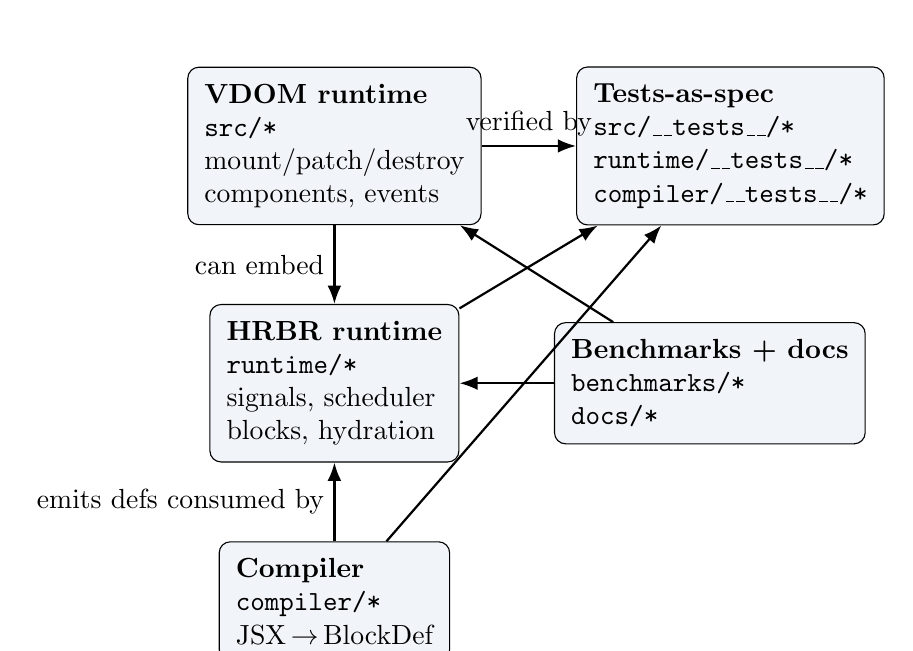
\begin{tikzpicture}[
  node distance=10mm and 12mm,
  box/.style={draw, rounded corners, align=left, inner sep=6pt, fill=RelaxLight},
  arrow/.style={-Latex, thick}
]
\node[box] (src) {\textbf{VDOM runtime}\\\texttt{src/*}\\mount/patch/destroy\\components, events};
\node[box, right=of src] (tests) {\textbf{Tests-as-spec}\\\texttt{src/\_\_tests\_\_/*}\\\texttt{runtime/\_\_tests\_\_/*}\\\texttt{compiler/\_\_tests\_\_/*}};
\node[box, below=of src] (runtime) {\textbf{HRBR runtime}\\\texttt{runtime/*}\\signals, scheduler\\blocks, hydration};
\node[box, below=of runtime] (compiler) {\textbf{Compiler}\\\texttt{compiler/*}\\JSX\,$\rightarrow$\,BlockDef};
\node[box, right=of runtime] (bench) {\textbf{Benchmarks + docs}\\\texttt{benchmarks/*}\\\texttt{docs/*}};

\draw[arrow] (src) -- node[midway, above] {verified by} (tests);
\draw[arrow] (runtime) -- (tests);
\draw[arrow] (compiler) -- (tests);

\draw[arrow] (compiler) -- node[midway, left] {emits defs consumed by} (runtime);
\draw[arrow] (src) -- node[midway, left] {can embed} (runtime);
\draw[arrow] (bench) -- (runtime);
\draw[arrow] (bench) -- (src);
\end{tikzpicture}
\end{center}

The key idea: tests are the stable external contract, while the implementation is split into a flexible VDOM baseline and an optional compiled runtime.

Everything else exists to support one of these (docs, benchmarks, build tooling).

\subsection{Directory map (first pass)}
This repository is split into a few major areas:

\begin{itemize}
  \item \texttt{src/}: the Relax.js Virtual DOM runtime.
  \item \texttt{runtime/}: an experimental runtime (HRBR) based on signals, scheduling, and compiled blocks.
  \item \texttt{compiler/}: a compiler/transform that converts a JSX subset into HRBR block definitions.
  \item \texttt{benchmarks/}: a browser harness to compare performance.
  \item \texttt{docs/}: design notes and whitepapers.
\end{itemize}

Two more folders matter when you're thinking about correctness:

\begin{itemize}
  \item \texttt{src/\_\_tests\_\_/}: the VDOM runtime spec.
  \item \texttt{runtime/\_\_tests\_\_/} and \texttt{compiler/\_\_tests\_\_/}: the HRBR + compiler spec.
\end{itemize}

\section{The constraint that shapes everything: DOM correctness in jsdom}
Almost every implementation choice is constrained by one hard rule:

\begin{quote}
The runtime must be correct in a headless DOM (jsdom), and tests are the contract.
\end{quote}

That affects:

\begin{itemize}
  \item Attribute vs property behavior (inputs/selects are tricky in jsdom).
  \item Event binding and cleanup.
  \item Diff algorithms (keyed moves must preserve node identity).
\end{itemize}

\subsection{Why jsdom is a meaningful constraint}
jsdom is \emph{not} a full browser, and that is exactly why it is useful here.
If your runtime depends on unspecified browser behavior or timing quirks, your test suite will become flaky.

Instead, tests in this repo focus on:

\begin{itemize}
  \item DOM structure (\texttt{innerHTML})
  \item identity (whether an element is reused or replaced)
  \item cleanup (event listeners and references are removed)
\end{itemize}

This shapes file boundaries: many helpers exist to make DOM updates deterministic and assertable.

\section{How to read code in this repo (recommended path)}
When you see a source file, immediately find its tests. That's the spec.

Recommended reading order:

\begin{enumerate}
  \item \texttt{src/index.ts} (public exports)
  \item \texttt{src/h.ts} (VNode model)
  \item \texttt{src/mount-dom.ts} (mount)
  \item \texttt{src/patch-dom.ts} (patch)
  \item \texttt{src/destroy-dom.ts} (cleanup)
  \item \texttt{src/component.ts} (components)
\end{enumerate}

\subsection{A second reading path: follow a user action}
The fastest way to build intuitions is to follow a single user interaction end-to-end.
For example: ``typing in an input and clicking a button adds a todo''.

You can trace that across:

\begin{itemize}
  \item event normalization: \texttt{src/events.ts}
  \item component event binding: \texttt{src/dispatcher.ts} and \texttt{src/component.ts}
  \item scheduling: \texttt{src/scheduler.ts} (\texttt{nextTick()})
  \item patching: \texttt{src/patch-dom.ts}
\end{itemize}

Doing this with the tests open beside you is the theme of this book.

\section{A concrete example: createApp() is tiny on purpose}
	exttt{createApp()} exists so the user has a simple lifecycle API.
The full file is short: \texttt{src/app.ts}.

Key behavior:

\begin{itemize}
  \item It creates a root VNode with \texttt{h(RootComponent, props)}.
  \item It mounts it once.
  \item It can unmount and fully cleanup.
\end{itemize}

\subsection{Code reference}
See \texttt{src/app.ts}. The central calls are \texttt{mountDOM(...)} and \texttt{destroyDOM(...)}.

\subsection{Test reference (what proves the contract)}
The high-level application lifecycle is specified by \texttt{src/\_\_tests\_\_/app.test.ts}.
This test file shows a full mount-to-interaction flow:

\begin{itemize}
  \item It mounts the app.
  \item It waits for async work with \texttt{await nextTick()}.
  \item It simulates user input by setting \texttt{input.value} and dispatching an \texttt{input} event.
  \item It simulates clicks via \texttt{button.click()}.
  \item It asserts DOM structure with \verb|singleHtmlLine`...`|.
\end{itemize}

That single test is a great ``reading harness'' for learning how Relax wires components + events + patching.

\section{Project constraint: small API surface}
Relax exports only a few primitives (h, fragments, components, scheduler).
Everything else is internal. That keeps the library small and also makes the tests more important.

\subsection{Where to see the supported surface area}
The public exports are in \texttt{src/index.ts} and mirrored by the \texttt{exports} map in \texttt{package.json}.

In other words:

\begin{itemize}
  \item if it's not in \texttt{src/index.ts}, it's not a stable public API
  \item tests are free to depend on internals, but users shouldn't
\end{itemize}

This book leans on that design: we can explain the internals without promising them as user-facing contracts.

\section{Tests: how this repo measures correctness}
This repository uses Vitest with a jsdom environment.
The configuration lives in \texttt{vitest.config.js}:

\begin{itemize}
  \item test patterns: \texttt{**/\_\_tests\_\_/**/*.test.ts(x)}
  \item reporters: verbose (good for learning)
  \item environment: jsdom
\end{itemize}

\subsection{The single most important helper: singleHtmlLine}
Many tests assert against HTML strings.
If you try to compare raw multi-line template literals to \texttt{innerHTML}, whitespace will fight you.

This repo solves that in \texttt{src/\_\_tests\_\_/utils.ts} with \texttt{singleHtmlLine()}:

\begin{itemize}
  \item it collapses whitespace
  \item it removes spaces between tags (for example, \texttt{>\textbackslash s+<} becomes \texttt{><})
  \item it trims
\end{itemize}

This is a micro-lesson in test design: you want assertions that are strict about structure, but forgiving about irrelevant formatting.

\subsection{Where to learn semantics fastest (test tour)}
If you're new to the codebase, these tests teach the contracts in the right order:

\begin{itemize}
  \item \texttt{src/\_\_tests\_\_/mount-dom.test.ts}:
    mount behavior, fragment behavior, saving \texttt{vdom.el} references.
  \item \texttt{src/\_\_tests\_\_/patch-dom.test.ts}:
    identity reuse vs replacement, attribute updates, keyed children, and edge cases.
  \item \texttt{src/\_\_tests\_\_/destroy-dom.test.ts}:
    cleanup and idempotency, especially ``remove event listeners''.
  \item \texttt{src/\_\_tests\_\_/component.test.ts}:
    component lifecycle, props/state updates, and event binding to the host component.
  \item \texttt{src/\_\_tests\_\_/jsx-react-syntax.test.tsx}:
    TSX compatibility contract (className/onClick/fragments/components).
\end{itemize}

Each of these will be revisited later in the book when we dive into the implementation files they protect.

\section{Mini-exercise}
Open these tests and write down what they prove (one sentence each). Then locate the implementation file they exercise.

\begin{itemize}
  \item \texttt{src/\_\_tests\_\_/app.test.ts}
  \item \texttt{src/\_\_tests\_\_/component.test.ts}
  \item \texttt{src/\_\_tests\_\_/mount-dom.test.ts}
  \item \texttt{src/\_\_tests\_\_/destroy-dom.test.ts}
\end{itemize}

If you can answer these, you're ready for Part II.

\section{Diagram: a "follow the tests" reading workflow}
When you don't know where to start, start from the tests and work backward to the implementation.

\begin{center}
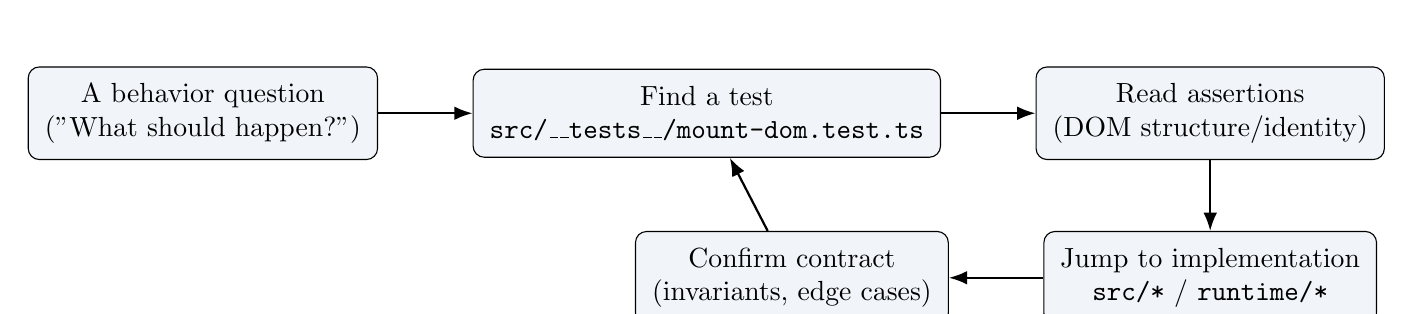
\begin{tikzpicture}[
  node distance=9mm and 12mm,
  box/.style={draw, rounded corners, align=center, inner sep=6pt, fill=RelaxLight},
  arrow/.style={-Latex, thick}
]
  \node[box] (fail) {A behavior question\\("What should happen?")};
  \node[box, right=of fail] (test) {Find a test\\\texttt{src/\_\_tests\_\_/mount-dom.test.ts}};
  \node[box, right=of test] (assert) {Read assertions\\(DOM structure/identity)};
  \node[box, below=of assert] (impl) {Jump to implementation\\\texttt{src/*} / \texttt{runtime/*}};
  \node[box, left=of impl] (confirm) {Confirm contract\\(invariants, edge cases)};

  \draw[arrow] (fail) -- (test);
  \draw[arrow] (test) -- (assert);
  \draw[arrow] (assert) -- (impl);
  \draw[arrow] (impl) -- (confirm);
  \draw[arrow] (confirm) -- (test);
\end{tikzpicture}
\end{center}

This loop is also how you safely add features: you extend the spec (tests) and then evolve the implementation.

\section{Online resources}
This chapter is about reading \emph{this repo}, but a few external references help explain why these constraints and structures are common.

\begin{itemize}
  \item DOM living standard (event/bubbling/capturing model):
    \href{https://dom.spec.whatwg.org/}{WHATWG DOM Standard}.
  \item Event handling basics and differences between properties vs attributes:
    \href{https://developer.mozilla.org/en-US/docs/Web/API/EventTarget/addEventListener}{MDN: addEventListener},
    \href{https://developer.mozilla.org/en-US/docs/Web/API/HTMLElement}{MDN: HTMLElement}.
  \item Testing DOM in Node:
    \href{https://vitest.dev/guide/}{Vitest Guide},
    \href{https://github.com/jsdom/jsdom}{jsdom}.
  \item Module packaging and exports maps:
    \href{https://nodejs.org/api/packages.html#packages_exports}{Node.js docs: \texttt{exports}}.
\end{itemize}

For formal citations, you can map key links into the backmatter \texttt{References} list in \texttt{book/main.tex}.

\chapter{TypeScript + JSX prerequisites}

\section{The goal}
Relax.js supports writing UI in TSX/JSX with a React-like syntax.
But remember: JSX is only syntax.
It becomes function calls (or, in TypeScript's modern mode, calls to a small ``JSX runtime'' module).

In Relax, the important function is still \texttt{h()} from \texttt{src/h.ts}.
The TSX layer exists to make authoring more ergonomic and familiar.

This chapter answers four practical questions:

\begin{enumerate}
  \item What does TypeScript emit for TSX in this repo?
  \item Where is the TSX runtime implemented (and what does it do)?
  \item Which React-like conveniences are supported (and which are not)?
  \item How do tests lock the TSX contract in place?
\end{enumerate}

\section{How TSX works in this repository (TypeScript configuration)}
The TSX behavior in this repo is primarily defined in \texttt{tsconfig.json}:

\begin{itemize}
  \item \texttt{jsx: "react-jsx"}
  \item \texttt{jsxImportSource: "relax-jsx"}
\end{itemize}

This combination means:

\begin{itemize}
  \item You \emph{do not} configure a global JSX factory function.
  \item TypeScript emits imports from \texttt{relax-jsx/jsx-runtime} (and sometimes \texttt{relax-jsx/jsx-dev-runtime}).
\end{itemize}

So the contract becomes very clean:
``TSX syntax must compile into objects that Relax can mount/patch/destroy.''

\section{Two JSX styles youll see}

\subsection{Direct VDOM authoring}
You can write VNodes manually:

\begin{lstlisting}[style=relax,language=JavaScript]
import { h, hFragment } from 'relax.js'

const view = hFragment([
  h('h1', {}, ['Hello']),
  h('button', { on: { click: () => console.log('clicked') } }, ['Click'])
])
\end{lstlisting}

\subsection{React-like TSX authoring}
TypeScript can compile TSX into calls to a configured JSX runtime.
This repo uses a React-like authoring style where:

\begin{itemize}
  \item \texttt{className} maps to Relaxs \texttt{class}.
  \item \texttt{onClick} maps to Relaxs event prop form (internally becomes \texttt{on: \{ click: fn \}}).
  \item Fragments (\texttt{<>...</>}) are supported.
\end{itemize}

There's an important nuance here:

\begin{quote}
Relax supports both ``native'' Relax props (like \texttt{class} and \texttt{on: \{ click: ... \}}) \emph{and} React-like compatibility props (like \texttt{className} and \texttt{onClick}).
\end{quote}

This design keeps the underlying runtime simple (it only needs to understand one internal prop shape) while letting TSX authoring feel familiar.

\section{The Relax JSX runtime (the real implementation)}
The TSX runtime lives in \texttt{relax-jsx/jsx-runtime.ts}.
It's intentionally tiny.

At a high level it does four jobs:

\begin{enumerate}
  \item Normalizes \texttt{children} to an array.
  \item Applies React-like prop compatibility:
    \begin{itemize}
      \item \texttt{className -> class}
      \item \texttt{onClick/onInput/... -> on: \{ click/input/... \}}
    \end{itemize}
  \item Threads the optional \texttt{key} through into Relax props.
  \item Delegates to Relax's real VDOM constructors:\
    	exttt{h(type, props, children)} or \texttt{hFragment(children)}.
\end{enumerate}

\subsection{Fragments: why \texttt{Fragment} is exported}
In the modern TS transform, fragments compile to a special ``Fragment'' value.
Relax's JSX runtime exports:

\begin{itemize}
  \item \texttt{export const Fragment = hFragment as any}
\end{itemize}

Then \texttt{jsxImpl()} checks whether the element type is \texttt{Fragment} and returns \texttt{hFragment(children)}.
That makes fragment VNodes indistinguishable from ones created explicitly via \texttt{hFragment()}.

\subsection{Dev runtime: jsxDEV}
Tooling sometimes emits \texttt{jsxDEV} calls in development builds.
This repo includes \texttt{relax-jsx/jsx-dev-runtime.ts}, which simply re-exports \texttt{Fragment}, \texttt{jsx}, and \texttt{jsxs}, and provides \texttt{jsxDEV(...)} as an alias to \texttt{jsx(...)}.

This is not a performance hack; it's a compatibility bridge so Vite/Vitest can run TSX code in different modes.

\section{Tests as spec}
The definitive spec for supported TSX/JSX features lives in:

\begin{itemize}
  \item \texttt{src/__tests__/jsx-tsx.test.ts}
  \item \texttt{src/__tests__/jsx-react-syntax.test.tsx}
\end{itemize}

\subsection{Test 1: TSX can mount via the Relax JSX runtime}
	exttt{src/__tests__/jsx-tsx.test.ts} is the smallest end-to-end proof:

\begin{itemize}
  \item It imports and runs \texttt{examples/jsx/hello.tsx}.
  \item That example defines a component whose \texttt{render()} returns TSX.
  \item It mounts using \texttt{createApp()}, waits \texttt{nextTick()}, and returns \texttt{innerHTML}.
\end{itemize}

If this test fails, it usually means one of these broke:

\begin{itemize}
  \item TS didn't resolve \texttt{relax-jsx/jsx-runtime} the way we expect (config/alias problem).
  \item The TSX runtime produced VNodes in a shape \texttt{mountDOM()} doesn't handle.
\end{itemize}

\subsection{Test 2: React-like conveniences are supported}
	exttt{src/__tests__/jsx-react-syntax.test.tsx} is a feature matrix.
It's intentionally written as ``contracts'' in a comment at the top of the file.

It specifies (and proves) things like:

\begin{itemize}
  \item intrinsic elements accept \texttt{id}, \texttt{className}, and text children
  \item fragments (\texttt{<>...</>}) work
  \item \texttt{onClick} attaches a DOM click handler
  \item list rendering via \texttt{items.map(...)} works (including \texttt{key})
  \item patching TSX trees updates DOM without reconstructing the whole host
  \item TSX works for Relax components created via \texttt{defineComponent()}
\end{itemize}

This test file is a great example of how to design compatibility: pick the exact subset you want, and encode it as executable assertions.

\section{Whats not the same as React}
Even though the syntax is familiar, semantics are Relaxs:

\begin{itemize}
  \item Components are created via \texttt{defineComponent()}.
  \item The event binding model binds handlers to the host component instance.
  \item Slots in Relax are a component feature (external/default content), not React children.
\end{itemize}

\subsection{Practical limitations of the TSX subset}
This repo intentionally does \emph{not} try to be a full React clone.
Two examples:

\begin{itemize}
  \item The TSX runtime only rewrites ``event props'' when the value is a function.
    If you pass non-function values to \texttt{onClick}, you should expect it to behave as a normal prop.
  \item ``React children'' as a conceptual model is not the point.
    In Relax, children are just VNodes (or arrays of VNodes) passed to \texttt{h()}.
\end{itemize}

The tests are the source of truth for what is supported.
If you'd like to extend the supported subset, the safest workflow is:

\begin{enumerate}
  \item Add a failing test first in \texttt{src/__tests__/jsx-react-syntax.test.tsx}.
  \item Update \texttt{relax-jsx/jsx-runtime.ts} to normalize the new case.
  \item Ensure mount/patch/destroy tests still pass.
\end{enumerate}

\section{Mini-exercise}
Read \texttt{src/__tests__/jsx-react-syntax.test.tsx} and answer:

\begin{enumerate}
  \item How are fragments compiled?
  \item How are events passed?
  \item How do components appear in JSX and how do props flow?
\end{enumerate}

Then open \texttt{relax-jsx/jsx-runtime.ts} and locate the exact code that implements each answer.

\section{Online resources (optional, citation-ready)}

\begin{itemize}
  \item TypeScript handbook: JSX (explains \texttt{react-jsx} and \texttt{jsxImportSource}):
    \href{https://www.typescriptlang.org/docs/handbook/jsx.html}{TypeScript: JSX}.
  \item React JSX runtime reference (useful for understanding why \texttt{jsx}/\texttt{jsxs}/\texttt{jsxDEV} exist):
    \href{https://react.dev/reference/react/jsx-runtime}{React docs: jsx-runtime}.
  \item Vite + Vitest module resolution (useful when JSX runtime imports fail):
    \href{https://vite.dev/guide/features.html#jsx}{Vite: JSX},
    \href{https://vitest.dev/guide/}{Vitest Guide}.
  \item DOM events (what an \texttt{onClick} becomes):
    \href{https://developer.mozilla.org/en-US/docs/Web/API/Element/click_event}{MDN: click event}.
\end{itemize}


% --- Part II (start) ---
\chapter{The VNode model (what the renderer \emph{really} consumes)}

In Chapter~3 we treated TSX as ``just syntax'' that boils down to calling \texttt{h()} and \texttt{hFragment()}.
This chapter is where I make that concrete.

If you strip Relax down to its bones, the renderer is a pair of functions:

\begin{itemize}
  \item \texttt{mountDOM(vdom, host)}: allocate DOM for a VNode tree.
  \item \texttt{patchDOM(oldVdom, newVdom, host)}: reconcile two VNode trees (reuse DOM).
\end{itemize}

Both functions only work if their input has a stable, predictable data shape.
That data shape is the \textbf{VNode model} in \texttt{src/h.ts}.

I like to describe \texttt{src/h.ts} as ``the type-level constitution of the renderer''.
If you understand the invariants enforced here, every later chapter gets easier.

\section{What you will build in your head}
By the end of this chapter you should be able to do these three things confidently:

\begin{enumerate}
  \item Read a random VNode object in a debugger and know what it means.
  \item Predict what \texttt{h('div', \{\}, ['x'])} returns (including text node normalization).
  \item Explain why \texttt{areNodesEqual()} is written the way it is and how it drives patching.
\end{enumerate}

\section{The one invariant I defend everywhere}
Relax keeps the VNode model intentionally small, and then makes the runtime depend on one invariant:

\begin{quote}
  \noindent\textbf{Invariant:} after creation, every value inside \texttt{VNode.children} is already a VNode.
  No raw strings, no raw numbers, no \texttt{null}, no \texttt{undefined}.
\end{quote}

This is not a ``nice-to-have''.
It's the thing that keeps \texttt{mountDOM()} and \texttt{patchDOM()} from degenerating into dozens of slow type checks.

\section{Why we need VNodes in the first place}
The DOM is mutable state.
The renderer's job is to move a lot of mutable state toward a desired UI with minimal work.

So we need a representation of ``desired UI'' that is:

\begin{itemize}
  \item \textbf{Pure data:} can be created without touching the DOM.
  \item \textbf{Stable:} has explicit node kinds and predictable fields.
  \item \textbf{Diffable:} can be compared against a previous version.
\end{itemize}

In Relax, that's the VNode.

\section{Why VNodes exist}
A virtual DOM implementation needs a stable, serializable representation of UI. In Relax, that representation is the \textbf{VNode}. The renderer can then be split into three big phases:

\begin{enumerate}
  \item \textbf{Create}: build a VNode tree (usually by calling \texttt{h()} directly, or indirectly via TSX as described in Chapter~3).
  \item \textbf{Mount}: allocate real DOM nodes for that tree (\texttt{src/mount-dom.ts}).
  \item \textbf{Patch}: reconcile an ``old tree'' with a ``new tree'' (\texttt{src/patch-dom.ts}), reusing as much DOM as possible.
\end{enumerate}

The ``create'' step is deceptively important: the more regular the VNode tree is, the less branching the mount/patch code needs.

\subsection*{Diagram: from render to real DOM}
The following diagram is the "wiring diagram" for the rest of Part~II. Every later chapter is basically "zooming in" on one box:

\begin{center}
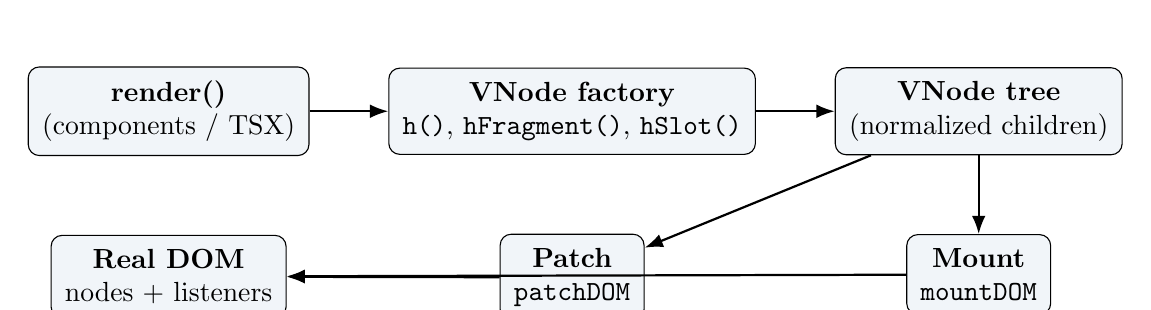
\begin{tikzpicture}[
  node distance=10mm,
  box/.style={draw,rounded corners,fill=RelaxLight,inner sep=5pt,align=center},
  arrow/.style={-Latex,thick}
]
  \node[box] (render) {\textbf{render()}\\(components / TSX)};
  \node[box, right=of render] (h) {\textbf{VNode factory}\\\texttt{h()}, \texttt{hFragment()}, \texttt{hSlot()}};
  \node[box, right=of h] (tree) {\textbf{VNode tree}\\(normalized children)};
  \node[box, below=of tree] (mount) {\textbf{Mount}\\\texttt{mountDOM}};
  \node[box, below=of h] (patch) {\textbf{Patch}\\\texttt{patchDOM}};
  \node[box, below=of render] (dom) {\textbf{Real DOM}\\nodes + listeners};

  \draw[arrow] (render) -- (h);
  \draw[arrow] (h) -- (tree);
  \draw[arrow] (tree) -- (mount);
  \draw[arrow] (mount) -- (dom);
  \draw[arrow] (tree) -- (patch);
  \draw[arrow] (patch) -- (dom);
\end{tikzpicture}
\end{center}

If you keep this picture in mind, a lot of micro-details (like \texttt{vdom.el} back-references or \texttt{areNodesEqual}) stop feeling ad-hoc: they're glue that keeps the arrows valid.

\section{The VNode types: \texttt{DOM\_TYPES}}
Relax defines node kinds as string constants in \texttt{DOM\_TYPES} (\texttt{src/h.ts}):

\begin{itemize}
  \item \texttt{TEXT}: a text node (\texttt{TextVNode}).
  \item \texttt{ELEMENT}: an HTML/SVG element (\texttt{ElementVNode}).
  \item \texttt{FRAGMENT}: a list of siblings without an extra wrapper element (\texttt{FragmentVNode}).
  \item \texttt{COMPONENT}: a component constructor + props/children (\texttt{ComponentVNode}).
  \item \texttt{SLOT}: a placeholder for ``external children'' in component trees (\texttt{SlotVNode}).
  \item \texttt{HRBR}: a special vnode wrapping an HRBR ``mount factory'' (\texttt{HrbrVNode}).
\end{itemize}

Two details are worth calling out because they influence the rest of the runtime:

\begin{enumerate}
  \item \textbf{Not every VNode has a DOM element.} \texttt{TEXT} uses a real \texttt{Text} node (\texttt{el?: Text}). \texttt{ELEMENT} uses a real \texttt{HTMLElement} (\texttt{el?: HTMLElement}). But \texttt{FRAGMENT} is special: it represents multiple siblings, so it can't point at a single ``root node''.
  \item \textbf{Keys are part of identity.} You'll see \texttt{props.key} used later by the reconciliation algorithm to decide whether a node is ``the same logical thing''.
\end{enumerate}

\section{Contract: \texttt{h(tag, props, children)}}
Relax's primary constructor is \texttt{h()} (\texttt{src/h.ts}). It's intentionally close to ``hyperscript'' functions found in other VDOM systems.

When I'm writing a renderer, I want the constructors to be boring.
``Boring'' here means: strongly asserted inputs, aggressively normalized children, minimal implicit behavior.
Relax follows that.

\subsection*{Code: the actual \texttt{h()} contract in \texttt{src/h.ts}}
The implementation is short enough that you should read it end-to-end at least once:

\begin{lstlisting}[language=JavaScript]
export function h(tag: string | unknown, props: Record<string, unknown> = {}, children: unknown[] = []): ElementVNode | ComponentVNode {
  const type = typeof tag === 'string' ? DOM_TYPES.ELEMENT : DOM_TYPES.COMPONENT

  assert(
    typeof props === 'object' && !Array.isArray(props),
    '[vdom] h() expects an object as props (2nd argument)'
  )
  assert(
    Array.isArray(children),
    `[vdom] h() expects an array of children (3rd argument), but got '${typeof children}'`
  )

  return {
    tag: tag as any,
    props: props as ElementVNodeProps,
    type,
    children: mapTextNodes(withoutNulls(children as any[])) as VNode[],
  } as any
}
\end{lstlisting}

Two things to notice:

\begin{itemize}
  \item \textbf{Fast fail:} \texttt{assert(...)} catches incorrect usage immediately.
  \item \textbf{Normalization happens right here:} \texttt{withoutNulls(...)} and \texttt{mapTextNodes(...)} enforce the children invariant.
\end{itemize}

\subsection*{Inputs}
\begin{itemize}
  \item \texttt{tag}: either a string (intrinsic element like \texttt{div}) or a component constructor/function.
  \item \texttt{props}: \emph{must be a plain object}. Relax checks this using \texttt{assert(...)} and fails fast with a helpful message.
  \item \texttt{children}: \emph{must be an array}. This is also asserted.
\end{itemize}

\subsection*{Output}
\begin{itemize}
  \item If \texttt{typeof tag === 'string'}, \texttt{h()} produces an \texttt{ELEMENT} vnode.
  \item Otherwise it produces a \texttt{COMPONENT} vnode.
\end{itemize}

Even though Relax supports TSX, TSX still ends up calling this layer (via the \texttt{relax-jsx} runtime), so understanding \texttt{h()} is foundational.

\section{Child normalization: \texttt{withoutNulls()} + \texttt{mapTextNodes()}}
Relax does two child normalization passes inside \texttt{h()} and \texttt{hFragment()}:

\begin{enumerate}
  \item \textbf{Drop nullish children}: \texttt{withoutNulls(children)} removes \texttt{null} and \texttt{undefined} (see \texttt{src/utils/arrays.ts}). This means ``conditional children'' can be written as \texttt{show ? node : null}.
  \item \textbf{Map primitives to \texttt{TEXT} nodes}: \texttt{mapTextNodes()} converts \texttt{string | number | boolean | bigint | symbol} into \texttt{TextVNode} via \texttt{hString()}.
\end{enumerate}

\subsection*{Why normalize eagerly?}
Normalization at creation time is a performance and correctness tactic:

\begin{itemize}
  \item \textbf{Performance:} mount/patch are on the hot path; you want them to pay as little "figure out what this is" cost as possible.
  \item \textbf{Correctness:} by forcing children into a single representation (VNodes), you avoid accidental differences between "first render" and "update" paths.
  \item \textbf{Debuggability:} tests can assert on VNode shapes without having to include JS coercion rules.
\end{itemize}

You can see this philosophy reflected in the tests: instead of testing dozens of mount/patch branches for primitives, the test suite locks down the normalization helpers and then relies on the invariant.

This is one of those design choices that pays rent everywhere:

\begin{itemize}
  \item Mount code can check \texttt{vNode.type} and never needs to special-case ``child is a string''.
  \item Patch code can treat text nodes uniformly; it doesn't have to worry about coercion rules.
\end{itemize}

\section{Fragments: \texttt{hFragment(children)} and \texttt{extractChildren()}}
Fragments represent ``multiple siblings'' and are heavily used by TSX fragment syntax (\texttt{<>...</>}).

\subsection*{Constructing fragments}
	exttt{hFragment(vNodes)} asserts the input is an array, filters nullish children, and maps primitives to text nodes (exactly like \texttt{h()}).

\subsection*{Code: fragment constructor}
This is the whole function (again: boring on purpose):

\begin{lstlisting}[language=JavaScript]
export function hFragment(vNodes: unknown[]): FragmentVNode {
  assert(Array.isArray(vNodes), '[vdom] hFragment() expects an array of vNodes')

  return {
    type: DOM_TYPES.FRAGMENT,
    children: mapTextNodes(withoutNulls(vNodes as any[])) as VNode[],
  }
}
\end{lstlisting}

\subsection*{Flattening fragments}
Later, other parts of the runtime sometimes need to treat ``a tree that may contain fragments'' as a flat list (for example, when calculating insertion positions).
	exttt{extractChildren(vdom)} provides that flattening:

\begin{itemize}
  \item If it finds a fragment child, it recursively collects that fragment's children.
  \item Otherwise it includes the child as-is.
\end{itemize}

The unit test \texttt{extract children from a tree with fragments} in \texttt{src/\_\_tests\_\_/h.test.ts} is your executable spec for this behavior.

\subsection*{Code: the spec is literally an object equality}
This is a good example of what I mean by ``tests as documentation'':

\begin{lstlisting}[language=JavaScript]
test('extract children from a tree with fragments', () => {
  const vNode = h('div', {}, [
    'A',
    hFragment([
      hFragment([hString('B')]),
      hString('C'),
      hFragment([hString('D')]),
    ]),
    'E',
  ])
  const children = extractChildren(vNode)

  expect(children).toEqual([
    { type: DOM_TYPES.TEXT, value: 'A' },
    { type: DOM_TYPES.TEXT, value: 'B' },
    { type: DOM_TYPES.TEXT, value: 'C' },
    { type: DOM_TYPES.TEXT, value: 'D' },
    { type: DOM_TYPES.TEXT, value: 'E' },
  ])
})
\end{lstlisting}

Notice what this test gives us: a guarantee that fragments behave like ``transparent containers'' for the purposes of child lists.

\section{Slots: \texttt{hSlot(children)} as a component-level placeholder}
Slots are how Relax expresses ``children passed into a component'' without forcing the component to take opaque \texttt{children} and do manual array plumbing.

At the VNode level, a slot is just:

\begin{itemize}
  \item \texttt{type: DOM\_TYPES.SLOT}
  \item optional \texttt{children}: default content to use when no external children are provided.
\end{itemize}

Then, to connect slot VNodes to component semantics, \texttt{src/h.ts} keeps a small piece of module-scoped state: \texttt{hSlotCalled}.

\subsection*{Why the module flag exists}
When rendering a component, Relax needs to know whether the component output contained at least one slot. Rather than scanning the render output tree after the fact, Relax uses this fast signal:

\begin{enumerate}
  \item \texttt{hSlot()} sets \texttt{hSlotCalled = true}.
  \item Component rendering checks \texttt{didCreateSlot()}.
  \item If a slot was created, the runtime calls the slot-filling algorithm (\texttt{src/slots.ts}) and then \texttt{resetDidCreateSlot()} to avoid leaking the flag into unrelated renders.
\end{enumerate}

This is one of Relax's ``tiny global state'' trade-offs: it keeps render fast and simple, but it also means slot creation is effectively a side-effect.

\subsection*{What the tests prove}
The best way to internalize slot semantics is to read \texttt{src/\_\_tests\_\_/component-slots.test.ts}. A few key cases:

\begin{itemize}
  \item \textbf{External content wins:} A component that renders \texttt{hSlot()} will receive the parent's children in that position.
  \item \textbf{Default content:} \texttt{hSlot([ ...default ])} is used when the parent provides no children.
  \item \textbf{Empty slot:} if there's no external content and no default content, the slot becomes empty (the test asserts \texttt{<div></div>}).
  \item \textbf{Conditional slots:} slot nodes can appear/disappear across re-renders, and patching handles it.
\end{itemize}

\section{HRBR interop: \texttt{hBlock(mount)} and VDOM identity}
HRBR (the compiled ``block'' runtime) needs to integrate into the same mounting/patching pipeline as regular VNodes. Relax does that by wrapping an HRBR mount factory in an \texttt{HRBR} vnode:

\begin{itemize}
  \item \texttt{hBlock(mount)} returns \texttt{\{ type: DOM\_TYPES.HRBR, mount \}}.
  \item Mounting creates a host element region and calls \texttt{mount(host)}.
  \item The returned instance exposes at least \texttt{destroy()}, and may expose \texttt{update()} / \texttt{dispose()}.
\end{itemize}

There's an important identity rule here, and the repo encodes it explicitly in \texttt{areNodesEqual()} (\texttt{src/nodes-equal.ts}):

\begin{quote}
  	extbf{HRBR vnode identity} is defined by mount factory identity: \texttt{old.mount === new.mount}.
\end{quote}

That single line is the difference between:

\begin{itemize}
  \item \textbf{Patch preserves instance:} stable mount function keeps the same HRBR instance.
  \item \textbf{Patch remounts:} new mount function destroys and mounts a fresh instance.
\end{itemize}

\subsection*{What the HRBR tests prove}
Read \texttt{src/\_\_tests\_\_/hrbr-integration.test.ts} as the contract:

\begin{itemize}
  \item \textbf{Mount and destroy:} an HRBR block returned from a VDOM component mounts into the DOM and gets destroyed on \texttt{destroyDOM}.
  \item \textbf{Event semantics:} HRBR event slots bind handler \texttt{this} to the host Relax component instance (the test asserts \texttt{calls[0].thisArg === vdom.component}).
  \item \textbf{Patch behavior:} stable vs. changing mount factory identity changes whether the HRBR instance is preserved.
\end{itemize}

This is a great example of the book's theme: treat tests as executable documentation.

\section{VNode identity and diffing: a preview}
This chapter is about creation, but VNode shape is designed with patching in mind. The function \texttt{areNodesEqual()} (\texttt{src/nodes-equal.ts}) shows you the identity rules Relax uses later:

\subsection*{Code: \texttt{areNodesEqual()} is tiny, but it's a design statement}
Read this function carefully.
Everything in patching depends on this decision about identity:

\begin{lstlisting}[language=JavaScript]
export function areNodesEqual(oldNode: any, newNode: any) {
  if (oldNode.type !== newNode.type) {
    return false
  }

  if (oldNode.type === DOM_TYPES.HRBR) {
    return oldNode.mount === newNode.mount
  }

  if (oldNode.type === DOM_TYPES.TEXT) {
    return true
  }

  if (oldNode.type === DOM_TYPES.ELEMENT) {
    return oldNode.tag === newNode.tag && oldNode.props?.key === newNode.props?.key
  }

  if (oldNode.type === DOM_TYPES.COMPONENT) {
    return oldNode.tag === newNode.tag && oldNode.props?.key === newNode.props?.key
  }

  return true
}
\end{lstlisting}

From a systems perspective, this is the policy wall between ``update in place'' and ``destroy + remount''.
If \texttt{areNodesEqual(old, next)} returns \texttt{false}, patching treats it as a different logical node and re-creates DOM / component instances.

\subsection*{Tests as spec: identity rules are enumerated}
The tests in \texttt{src/\_\_tests\_\_/node-equals.test.ts} are effectively a checklist:

\begin{itemize}
  \item Text nodes: always equal (value patches, identity doesn't change).
  \item Fragments: always equal.
  \item Elements: equal if tag matches, and key matches when present.
  \item Components: equal if constructor matches, and key matches when present.
\end{itemize}

This is why I keep the function small: it's easier to reason about and easier to lock down with tests.

\begin{itemize}
  \item text nodes: always equal (Relax patches text by updating value rather than replacing node type)
  \item fragments: always equal
  \item elements: equal if tag matches and \texttt{props.key} matches
  \item components: equal if constructor matches and \texttt{props.key} matches
  \item HRBR: equal if mount factory function is the same
\end{itemize}

The tests in \texttt{src/\_\_tests\_\_/node-equals.test.ts} enumerate these cases in small, sharp assertions.

\section{Mini-exercises}
\begin{enumerate}
  \item \textbf{Read like a maintainer:} In \texttt{src/\_\_tests\_\_/h.test.ts}, locate the test named \texttt{"h() maps 'number', 'boolean', 'bigint', and 'symbol' values to text vNodes"}. Explain (to yourself) why \texttt{Symbol(5)} becomes the string \texttt{"Symbol(5)"}.
  \item \textbf{Write a new invariant test:} Add a small test that asserts \texttt{h('div', {}, [null, undefined, 'x']).children.length === 1}. (This should already be true, but the test helps lock the behavior down.)
  \item \textbf{Identity thought experiment:} Why do you think Relax treats text nodes as ``always equal''? What does that allow \texttt{patchDOM()} to do as an optimization?
\end{enumerate}

\section{Online resources}
This chapter describes patterns that show up across many UI runtimes. These references help if you want to compare Relax's choices to other ecosystems:

\begin{itemize}
  \item Hyperscript and virtual node factories (conceptual background): \href{https://github.com/hyperhype/hyperscript}{https://github.com/hyperhype/hyperscript}
  \item DOM node types (Text vs Element) on MDN: \href{https://developer.mozilla.org/en-US/docs/Web/API/Node/nodeType}{https://developer.mozilla.org/en-US/docs/Web/API/Node/nodeType}
  \item React's reconciliation keys (why \texttt{key} exists): \href{https://react.dev/learn/rendering-lists}{https://react.dev/learn/rendering-lists}
  \item Web Components slots (a parallel mental model for ``default vs external'' content): \href{https://developer.mozilla.org/en-US/docs/Web/API/Web_components/Using_templates_and_slots}{\url{https://developer.mozilla.org/en-US/docs/Web/API/Web_components/Using_templates_and_slots}}
\end{itemize}

\chapter{Mounting DOM (\texttt{src/mount-dom.ts})}

This chapter is about the first half of the renderer: taking the data structures from \texttt{src/h.ts} and producing real DOM nodes.

In Relax theres a clean separation:

\begin{itemize}
  \item \textbf{Creation} builds VNode trees (Chapter~4).
  \item \textbf{Mounting} turns VNodes into DOM and stores back-references (this chapter).
  \item \textbf{Patching} reconciles trees (Chapter~8).
  \item \textbf{Destroying} cleans up listeners / component instances / HRBR blocks (Chapter~9).
\end{itemize}

The entry point is \texttt{mountDOM(vdom, parentEl, index?, hostComponent?)} in \texttt{src/mount-dom.ts}.

\section{Contract: \texttt{mountDOM}}

\subsection*{Inputs}
\begin{itemize}
  \item \texttt{vdom}: a VNode (one of the \texttt{DOM\_TYPES}).
  \item \texttt{parentEl}: the DOM element where the node should be inserted. This must be non-null.
  \item \texttt{index} (optional): insert position inside \texttt{parentEl.childNodes}.
  \item \texttt{hostComponent} (optional): the component instance that should become \texttt{this} for event handlers.
\end{itemize}

\subsection*{Outputs / side-effects}
\begin{itemize}
  \item Inserts DOM into \texttt{parentEl}.
  \item Mutates the vnode: for most node types, \texttt{vdom.el} becomes a back-reference to the created DOM.
  \item For elements, saves listener cleanup hooks on \texttt{vdom.listeners}.
  \item For components, creates and stores \texttt{vdom.component}.
\end{itemize}

\subsection*{Failure modes}
\begin{itemize}
  \item If \texttt{parentEl == null}, it throws \texttt{[mountDOM] Parent element is null}.
  \item If \texttt{vdom.type} doesnt match any known tag in \texttt{DOM\_TYPES}, it throws \texttt{Can't mount DOM of type: ...}.
\end{itemize}

The tests in \texttt{src/__tests__/mount-dom.test.ts} include a couple of ``guardrail'' cases that assert these errors exist.

\section{The central pattern: dispatch by \texttt{vdom.type}}
	exttt{mountDOM()} is a type-dispatcher. In code its a \texttt{switch (vdom.type)} that delegates to one helper per vnode kind:

\begin{itemize}
  \item \texttt{createTextNode} for \texttt{DOM\_TYPES.TEXT}
  \item \texttt{createElementNode} for \texttt{DOM\_TYPES.ELEMENT}
  \item \texttt{createFragmentNodes} for \texttt{DOM\_TYPES.FRAGMENT}
  \item \texttt{createComponentNode} for \texttt{DOM\_TYPES.COMPONENT}
  \item \texttt{createHrbrNode} for \texttt{DOM\_TYPES.HRBR}
\end{itemize}

This is not just an organizational trick: it is what makes patching symmetric later. Chapter~8 will mirror this shape with a patch dispatcher.

\section{Text nodes: \texttt{createTextNode}}
For \texttt{TextVNode}, mounting is:

\begin{enumerate}
  \item Create a real text node: \texttt{document.createTextNode(vdom.value)}.
  \item Store a stable back-pointer: \texttt{vdom.el = textNode}.
  \item Insert it into the parent using \texttt{insert(textNode, parentEl, index)}.
\end{enumerate}

\subsection*{What the tests prove}
	exttt{src/__tests__/mount-dom.test.ts} contains two small tests that act like a contract:

\begin{itemize}
  \item \texttt{mount a text element in a host element}: asserts the DOM contains \texttt{hello}.
  \item \texttt{save the created text element in the vdom}: asserts \texttt{vdom.el} is a \texttt{Text} instance and points at the right content.
\end{itemize}

Read those tests as: ``If we ever refactor mounting, these properties must remain true or patching/destroying will become unreliable.''

\section{Element nodes: \texttt{createElementNode} and the props/events split}
For \texttt{ElementVNode}, Relax mounts in a deliberate order:

\begin{enumerate}
  \item Create \texttt{const element = document.createElement(tag)}.
  \item Apply props and events via \texttt{addProps(element, vdom, hostComponent)}.
  \item Store \texttt{vdom.el = element}.
  \item Mount children into \texttt{element} (recursively via \texttt{mountDOM(child, element, null, hostComponent)}).
  \item Insert the final element into the parent.
\end{enumerate}

The most important concept here is that Relax treats events specially.

\subsection{\texttt{addProps}: extracting attrs vs. events}
	exttt{addProps()} calls \texttt{extractPropsAndEvents(vdom)} (from \texttt{src/utils/props.ts}). The return value is split into:

\begin{itemize}
  \item \textbf{attrs}: everything that becomes DOM attributes/properties (\texttt{id}, \texttt{class}, \texttt{style}, \texttt{data-*}, etc).
  \item \textbf{events}: the event map stored under \texttt{props.on}.
\end{itemize}

Then mounting wires two subsystems:

\begin{itemize}
  \item \texttt{addEventListeners(events, el, hostComponent)} returns a map of cleanup functions; this is saved as \texttt{vdom.listeners}.
  \item \texttt{setAttributes(el, attrs)} applies the non-event attributes.
\end{itemize}

That \texttt{vdom.listeners} back-reference is critical later in Chapter~9: destroying uses it to remove listeners even if the vnode is no longer in the DOM.

\subsection*{What the tests prove}
The tests in \texttt{src/__tests__/mount-dom.test.ts} cover a small but meaningful matrix:

\begin{itemize}
  \item \textbf{attributes:} id, class, list-of-classes
  \item \textbf{style:} a style object becomes an inline style string
  \item \textbf{events:} clicking the element calls the handler and \texttt{vdom.listeners} is populated
\end{itemize}

These are not ``just tests''they are a spec for how Relax converts the VNode \texttt{props} object into real DOM behavior.

\section{Event handler binding: the meaning of \texttt{hostComponent}}
	exttt{mountDOM()} accepts an optional \texttt{hostComponent} argument, which gets threaded into \texttt{createElementNode(...)} and ultimately into \texttt{addEventListeners(...)}.

The intent is: when a component mounts elements, those element event handlers should run with \texttt{this === componentInstance} so handler methods can mutate component state.

\subsection*{What the tests prove}
The test \texttt{where there is a host component, the event handlers are bound to it} builds a fragment containing two buttons and passes a plain object \texttt{comp = \{ count: 5 \}} as the host. Both click handlers increment \texttt{this.count}. The assertions show two things:

\begin{itemize}
  \item the same host is used for nested mounts (a button nested inside a div still binds \texttt{this} correctly)
  \item binding is not limited to direct children
\end{itemize}

This is a key piece of ``component semantics'' even though its implemented entirely inside the mounting layer.

\section{Fragments: \texttt{createFragmentNodes} and insertion indices}
Fragments are the trickiest type to mount because a fragment is ``many nodes''.

Relaxs move is simple:

\begin{quote}
  A fragment vnode stores \texttt{vdom.el = parentEl}.
\end{quote}

That is, a fragment doesnt own a DOM node. Instead, it keeps a reference to the container it was mounted in.

\subsection{The index problem}
When mounting into an explicit \texttt{index}, you want fragment children to appear starting at that position.
But as soon as you insert the first child, the parents \texttt{childNodes} list changes, and the next childs target index must shift.

Relax solves this by maintaining a local counter \texttt{idx}:

\begin{itemize}
  \item If \texttt{idx == null}, it just appends each child and doesnt care.
  \item Otherwise, after mounting each child, it increments \texttt{idx} by the number of DOM nodes that child contributed.
\end{itemize}

The ``how many DOM nodes did this child contribute?'' logic is where fragments and components matter:

\begin{itemize}
  \item child fragment: contributes \texttt{child.children.length}
  \item child component: contributes \texttt{child.component.elements.length}
  \item other nodes: contribute \texttt{1}
\end{itemize}

This design implies a subtle contract with the component implementation: component instances must maintain an \texttt{elements} array listing the DOM nodes they own.
Youll revisit that in the component lifecycle chapters.

\subsection*{What the tests prove}
	exttt{src/__tests__/mount-dom.test.ts} contains several important fragment tests:

\begin{itemize}
  \item \texttt{mount a fragment in a host element} and \texttt{mount a fragment inside a fragment...}: show that fragments flatten naturally at mount time.
  \item \texttt{all nested fragments el references point to the parent element}: asserts the design choice \texttt{fragment.el === parentEl} even for nested fragments.
  \item A parametrized \texttt{test.each} suite (later in the file) checks insertion-index behavior for complex nested fragment/component scenarios.
\end{itemize}

\section{Components: \texttt{createComponentNode} and asynchronous \texttt{onMounted}}
Component mounting bridges VDOM to component instances.
The algorithm in \texttt{createComponentNode()} is:

\begin{enumerate}
  \item Split vnode props into \texttt{props} and \texttt{events} via \texttt{extractPropsAndEvents(...)}.
  \item Allocate the instance: \texttt{new Component(props, events, hostComponent)}.
  \item Store external children: \texttt{component.setExternalContent(vdom.children)}.
  \item Delegate to the component to mount itself: \texttt{component.mount(parentEl, index)}.
  \item Store \texttt{vdom.component = component}.
  \item Store \texttt{vdom.el = component.firstElement}.
\end{enumerate}

The last step is important: a component vnode cannot point to ``the component'' as a DOM node, so Relax points it at the first DOM element the component produced. Patching uses this to locate and replace component output.

\subsection{Lifecycle scheduling and the job queue}
Immediately after creating a component node, \texttt{mountDOM()} enqueues a lifecycle callback:

\begin{quote}
	exttt{enqueueJob(() => vdom.component.onMounted())}
\end{quote}

So \texttt{onMounted()} is intentionally asynchronous relative to ``the DOM nodes now exist''.
This approach avoids re-entrancy hazards (mount causing mount causing mount) and aligns with how many UI systems schedule lifecycle effects.

\subsection*{What the tests prove}
	exttt{src/__tests__/mount-dom.test.ts} exercises component creation and parent-child links:

\begin{itemize}
  \item \texttt{mount a component with props}: shows that props are passed in and the instance is stored.
  \item \texttt{mount a component with children}: shows that children can be used to build deeper trees.
  \item \texttt{mount a component with a parent component} and \texttt{child components keep a reference to their parent component}: show that \texttt{hostComponent} threads the parent/child relationship.
  \item \texttt{when a component with multiple elements is mounted, the vdom keeps a reference to the first element}: locks down the \texttt{vdom.el = firstElement} rule.
\end{itemize}

\section{HRBR interop: \texttt{createHrbrNode} and why \texttt{el} points to the host}
HRBR nodes are mounted by allocating a dedicated host container element:

\begin{itemize}
  \item Create a \texttt{<span>} host.
  \item Mark it with a dataset flag: \texttt{host.dataset.hrbr = '1'}.
  \item Insert the host into the parent.
  \item Call the mount factory: \texttt{instance = vdom.mount(host)}.
  \item Store \texttt{vdom.instance = instance}.
  \item Store \texttt{vdom.el = host} (and also \texttt{vdom.host = host}).
\end{itemize}

The comment in \texttt{src/mount-dom.ts} is worth repeating: \textbf{VDOM owns the host container, not the hosts first child.} Patch logic later locates nodes by \texttt{oldVdom.el}; if \texttt{el} pointed inside HRBR output, replacement/removal would get the wrong DOM index.

\subsection*{What the tests prove}
While the mounting tests live in \texttt{mount-dom.test.ts}, HRBR mounting is exercised via integration tests in \texttt{src/__tests__/hrbr-integration.test.ts}.
Those tests treat HRBR blocks as ``just another vnode type'' and assert:

\begin{itemize}
  \item the DOM output appears after mounting
  \item the block is destroyed when the VDOM is destroyed
  \item patching preserves vs remounts based on mount factory identity
\end{itemize}

\section{Insertion mechanics: \texttt{insert(el, parentEl, index)}}
Everything ultimately goes through \texttt{insert()}, which implements four rules:

\begin{itemize}
  \item \textbf{append:} if \texttt{index == null}, append.
  \item \textbf{reject negative indices:} if \texttt{index < 0}, throw.
  \item \textbf{append out-of-range:} if \texttt{index >= parent.childNodes.length}, append.
  \item \textbf{insertBefore otherwise:} insert before \texttt{childNodes[index]}.
\end{itemize}

The tests include a negative-index case (throws) and several index-sensitive fragment suites.

\section{Mini-exercises}
\begin{enumerate}
  \item Add a focused test to \texttt{mount-dom.test.ts} proving that mounting with an out-of-range index appends for element vnodes. (Youll be asserting the same rule \texttt{insert()} implements.)
  \item In \texttt{mount-dom.test.ts}, find the parameterized index tests and explain why nested components contribute \texttt{component.elements.length} to the index offset.
\end{enumerate}

\section{Online resources}
\begin{itemize}
  \item DOM basics: \texttt{document.createElement} (MDN): \href{https://developer.mozilla.org/en-US/docs/Web/API/Document/createElement}{https://developer.mozilla.org/en-US/docs/Web/API/Document/createElement}
  \item DOM basics: \texttt{Node.insertBefore} (MDN): \href{https://developer.mozilla.org/en-US/docs/Web/API/Node/insertBefore}{https://developer.mozilla.org/en-US/docs/Web/API/Node/insertBefore}
  \item DOM basics: \texttt{Node.appendChild} / \texttt{Element.append} (MDN): \href{https://developer.mozilla.org/en-US/docs/Web/API/Element/append}{https://developer.mozilla.org/en-US/docs/Web/API/Element/append}
  \item Event targets and listener binding (MDN): \href{https://developer.mozilla.org/en-US/docs/Web/API/EventTarget/addEventListener}{https://developer.mozilla.org/en-US/docs/Web/API/EventTarget/addEventListener}
  \item ``Why schedule effects'' background (Reacts mental model is a good reference even if implementation differs): \href{https://react.dev/learn/synchronizing-with-effects}{https://react.dev/learn/synchronizing-with-effects}
\end{itemize}

\chapter{Attributes, properties, classes, and styles (\texttt{src/attributes.ts})}

This chapter is the ``DOM edge'' chapter.
Mounting (Chapter~5) can create elements in a few lines, but \emph{correctly configuring those elements} is where UI libraries accumulate complexity.

Relax keeps its attribute system intentionally small: a handful of rules, continuously validated by broad jsdom test coverage.

\section{Why this chapter matters}
Browsers expose multiple mechanisms that look similar but behave differently:

\begin{enumerate}
  \item \textbf{DOM attributes}: strings stored in the element's attribute map (example: \texttt{el.getAttribute('id')}).
  \item \textbf{DOM properties}: live fields on the element object (example: \texttt{(input as any).value}).
  \item \textbf{Special cased fields}: \texttt{className} and \texttt{style} have their own APIs and behavior.
\end{enumerate}

\subsection*{Diagram: the attribute write decision (attribute vs property)}
\begin{center}
\begin{tikzpicture}[
  node distance=10mm and 16mm,
  box/.style={draw, rounded corners, align=left, inner sep=6pt, fill=RelaxLight},
  decision/.style={draw, diamond, aspect=2, align=center, inner sep=2pt, fill=RelaxLight},
  arrow/.style={-Latex, thick}
]
\node[box] (input) {Input\\\texttt{name, value}};
\node[decision, right=of input] (isnull) {\texttt{value == null}?};
\node[box, above right=of isnull] (remove) {\texttt{removeAttribute(el, name)}\\(also tries property\,=\,null)};
\node[decision, below right=of isnull] (isdata) {\texttt{name.startsWith('data-')}?};
\node[box, right=of isdata] (attr) {Write attribute\\\texttt{el.setAttribute(name, String(value))}};
\node[box, below=of attr] (prop) {Write property\\\texttt{(el as any)[name] = value}};

\draw[arrow] (input) -- (isnull);
\draw[arrow] (isnull) -- node[midway, above] {yes} (remove);
\draw[arrow] (isnull) -- node[midway, left] {no} (isdata);
\draw[arrow] (isdata) -- node[midway, above] {yes} (attr);
\draw[arrow] (isdata) -- node[midway, right] {no} (prop);
\end{tikzpicture}
\end{center}

This is the core policy tested by the big matrix in \texttt{src/\_\_tests\_\_/attributes.test.ts}: most names are treated as properties, while \texttt{data-*} is always an attribute.

If you set the wrong one, you can get subtle bugs. For instance, setting \texttt{value} as an attribute on \texttt{<input>} won't behave like setting the property in many scenarios.

Relax's pragmatic rule is:

\begin{quote}
  	extbf{Rule:} if the name starts with \texttt{data-}, set an \emph{attribute}; otherwise set a \emph{property}.
\end{quote}

You can see this rule directly in \texttt{setAttribute()} in \texttt{src/attributes.ts}.

\section{Contract: \texttt{setAttributes(el, attrs)}}
The top-level API is:

\begin{quote}
	exttt{setAttributes(el: HTMLElement, attrs: ElementVNodeProps)}
\end{quote}

This function is used during mount (Chapter~5) and also during patches when props change (Chapter~8).

\subsection*{Inputs}
\begin{itemize}
  \item \texttt{el}: a real DOM element.
  \item \texttt{attrs}: Relax's element props object (roughly: \texttt{id}, \texttt{class}, \texttt{style}, and anything else).
\end{itemize}

\subsection*{Behavior}
	exttt{setAttributes()} applies attributes in three phases:

\begin{enumerate}
  \item split out \texttt{class} and \texttt{style}
  \item delete \texttt{key} (VDOM identity only)
  \item for each remaining entry: \texttt{setAttribute(el, name, value)}
\end{enumerate}

\subsection*{Diagram: \texttt{setAttributes()} pipeline (split, normalize, apply)}
\begin{center}
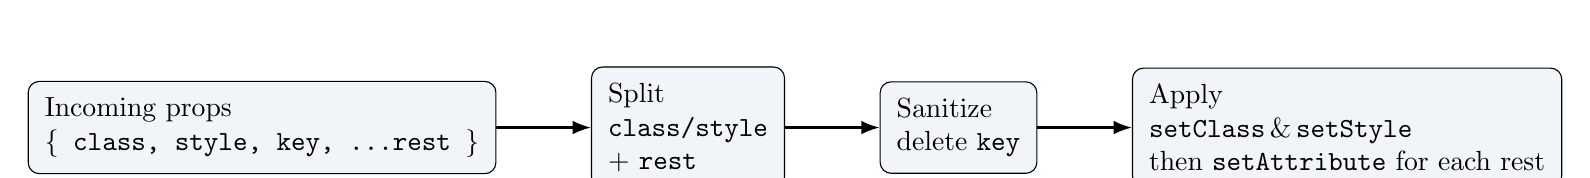
\begin{tikzpicture}[
  node distance=10mm and 12mm,
  box/.style={draw, rounded corners, align=left, inner sep=6pt, fill=RelaxLight},
  arrow/.style={-Latex, thick}
]
\node[box] (attrs) {Incoming props\\\texttt{\{ class, style, key, ...rest \}}};
\node[box, right=of attrs] (split) {Split\\\texttt{class/style}\\+ \texttt{rest}};
\node[box, right=of split] (sanitize) {Sanitize\\delete \texttt{key}};
\node[box, right=of sanitize] (apply) {Apply\\\texttt{setClass}\,\&\,\texttt{setStyle}\\then \texttt{setAttribute} for each rest};

\draw[arrow] (attrs) -- (split);
\draw[arrow] (split) -- (sanitize);
\draw[arrow] (sanitize) -- (apply);
\end{tikzpicture}
\end{center}

The important invariant here is that \texttt{key} never reaches the DOM, even if user code passes it.

\subsection{Important invariant: \texttt{key} is not a DOM attribute}
Relax uses \texttt{key} for diffing lists and stabilizing identity. It should never appear on the real DOM.

To enforce this, key removal happens in two places:

\begin{itemize}
  \item \texttt{src/attributes.ts}: deletes \texttt{otherAttrs.key}
  \item \texttt{src/utils/props.ts}: deletes \texttt{props.key} when extracting props/events
\end{itemize}

The duplication is intentional: it keeps each layer correct even if used in isolation.

\section{Class handling: replacement semantics}
Relax exposes \texttt{class} as either:

\begin{itemize}
  \item a string (example: \texttt{"foo bar"})
  \item an array of class tokens (example: \texttt{["foo", "bar"]})
\end{itemize}

Implementation detail (\texttt{setClass()} in \texttt{src/attributes.ts}):

\begin{itemize}
  \item it clears \texttt{el.className = ''}
  \item if \texttt{className} is a string, it assigns \texttt{el.className = className}
  \item if it's an array, it does \texttt{el.classList.add(...className)}
\end{itemize}

This makes class setting \textbf{replacement based}, not incremental diff. That's a conscious simplicity trade-off.

\subsection*{What the tests prove}
The first three tests in \texttt{src/\_\_tests\_\_/attributes.test.ts} provide the contract:

\begin{itemize}
  \item \texttt{setting a class from a string}
  \item \texttt{setting a class from an array}
  \item \texttt{updating the class} (proves replacement, not accumulation)
\end{itemize}

\section{Style handling: direct assignment}
Relax's \texttt{style} prop is a plain object:

\begin{quote}
	exttt{\{ style: \{ color: 'red', backgroundColor: 'blue' \} \}}
\end{quote}

For each \texttt{[name, value]} pair, \texttt{setAttributes()} calls \texttt{setStyle(el, name, value)}, which does a direct assignment:

\begin{quote}
	exttt{(el.style as any)[name] = value}
\end{quote}

Removal goes through \texttt{removeStyle()} which sets the field to \texttt{null}.

\subsection*{Diagram: class/style are special-cased, everything else is generic}
\begin{center}
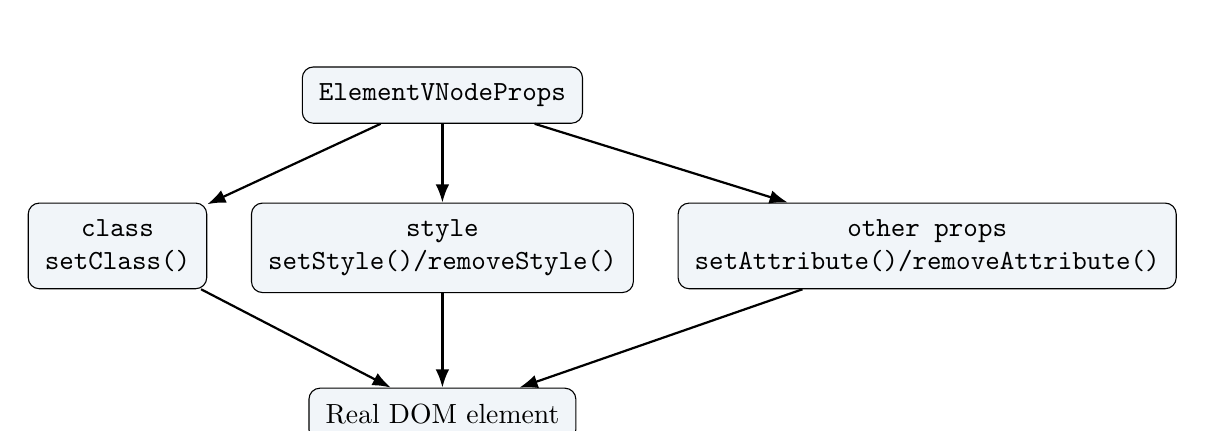
\begin{tikzpicture}[
  node distance=10mm and 12mm,
  box/.style={draw, rounded corners, align=center, inner sep=6pt, fill=RelaxLight},
  arrow/.style={-Latex, thick}
]
\node[box] (props) {\texttt{ElementVNodeProps}};
\node[box, below left=of props] (class) {\texttt{class}\\\texttt{setClass()}};
\node[box, below=of props] (style) {\texttt{style}\\\texttt{setStyle()/removeStyle()}};
\node[box, below right=of props] (rest) {\texttt{other props}\\\texttt{setAttribute()/removeAttribute()}};
\node[box, below=of style, yshift=-2mm] (dom) {Real DOM element};

\draw[arrow] (props) -- (class);
\draw[arrow] (props) -- (style);
\draw[arrow] (props) -- (rest);
\draw[arrow] (class) -- (dom);
\draw[arrow] (style) -- (dom);
\draw[arrow] (rest) -- (dom);
\end{tikzpicture}
\end{center}

One subtle consequence: \texttt{setAttributes()} does not diff old vs new style objects. If you call it twice, the second call only assigns the fields present in the second object. it does \emph{not} remove fields that were present previously unless you explicitly remove them.

\subsection*{What the tests prove}
	exttt{setting styles} and \texttt{updating styles} assert that style fields are applied by assignment and can coexist across multiple calls.

\section{The core rule: \texttt{setAttribute(el, name, value)}}
The function \texttt{setAttribute()} is the heart of the module:

\begin{enumerate}
  \item If \texttt{value == null} \textrightarrow{} call \texttt{removeAttribute(el, name)}.
  \item Else if \texttt{name.startsWith('data-')} \textrightarrow{} call \texttt{el.setAttribute(name, String(value))}.
  \item Else \textrightarrow{} write as a property: \texttt{(el as any)[name] = value}.
\end{enumerate}

This is where Relax chooses ``property first'' semantics. The benefit is correctness for form controls and boolean-ish fields.

\subsection*{What the tests prove: the matrix}
  exttt{src/\_\_tests\_\_/attributes.test.ts} is a deliberately wide matrix of real DOM behavior.

Highlights:

\begin{itemize}
  \item \textbf{Generic element properties:}
    	exttt{hidden}, \texttt{tabIndex} (including \texttt{tabIndex} removal resulting in \texttt{-1}).
  \item \textbf{Input type=text properties:}
    	exttt{value}, \texttt{placeholder}, \texttt{disabled}, \texttt{minLength}, \texttt{size}, and more.
  \item \textbf{Checkbox / radio:}
    	exttt{checked} is a property and removal resets to \texttt{false}.
  \item \textbf{Select:}
    setting \texttt{value} to a missing option results in \texttt{''}.
  \item \textbf{Anchors/buttons/spans:}
    properties like \texttt{href}, \texttt{disabled}, and \texttt{textContent} behave like live fields.
\end{itemize}

This test suite is doing an important job: it prevents ``helpful refactors'' from changing semantics that look equivalent but aren't.

\section{Removal: \texttt{removeAttribute(el, name)} and jsdom quirks}
Removing an attribute sounds simple but isn't.

Relax tries to clear both levels:

\begin{enumerate}
  \item it attempts to set the property to \texttt{null} inside a \texttt{try/catch}
  \item it always calls \texttt{el.removeAttribute(name)}
\end{enumerate}

The \texttt{try/catch} exists because some properties throw when assigned \texttt{null} (depending on element type and environment).
When that happens, Relax logs a warning:

\begin{quote}
	exttt{Failed to set "<name>" to null on <TAG>}
\end{quote}

That warning is not a test failure; it's a visibility aid for cases where property clearing is not permitted.

\section{Props vs events: \texttt{extractPropsAndEvents} (\texttt{src/utils/props.ts})}
Relax stores event handlers under \texttt{props.on}. Before mounting or constructing a component instance, it needs to split the two.

	exttt{extractPropsAndEvents(vdom)} does exactly that:

\begin{itemize}
  \item \texttt{events}: \texttt{vdom.props.on} (defaulting to \texttt{\{\}})
  \item \texttt{props}: everything else (and it deletes \texttt{key})
\end{itemize}

This split is used in two places you've already seen:

\begin{itemize}
  \item element mounting: \texttt{addEventListeners(events, el, hostComponent)} and \texttt{setAttributes(el, props)}
  \item component mounting: \texttt{new Component(props, events, hostComponent)}
\end{itemize}

\subsection*{What the tests prove}
  exttt{src/\_\_tests\_\_/props.test.ts} is intentionally small and crisp:

\begin{itemize}
  \item empty input yields empty outputs
  \item \texttt{key} is ignored
  \item non-event fields remain in \texttt{props}
  \item \texttt{on: \{...\}} becomes \texttt{events}
\end{itemize}

Treat these as invariants: if you ever change the VNode prop shape, these tests are the first alarm bell.

\section{Design notes (trade-offs)}
Relax's attribute model is intentionally simple:

\begin{itemize}
  \item it mostly treats prop names as property names
  \item it special-cases only \texttt{data-*}, \texttt{class}, and \texttt{style}
  \item it relies on a test matrix to ensure that simplicity doesn't break real DOM behavior
\end{itemize}

If you were extending Relax, likely next steps would be:

\begin{itemize}
  \item richer SVG support (namespaces and attribute/property differences)
  \item style diff/removal semantics (tracking old style object)
  \item explicit boolean attribute reflection rules (attribute presence vs property value)
\end{itemize}

\section{Mini-exercises}
\begin{enumerate}
  \item Add a new case to the matrix in \texttt{src/\_\_tests\_\_/attributes.test.ts} for \texttt{<textarea>} value behavior.
  \item Add a test that asserts \texttt{setAttributes(el, \{ key: 'x', id: 'y' \})} does not create a \texttt{key} attribute in the DOM.
\end{enumerate}

\section{Online resources}
\begin{itemize}
  \item Attributes vs. properties (MDN, conceptual background): \href{https://developer.mozilla.org/en-US/docs/Web/API/Element}{https://developer.mozilla.org/en-US/docs/Web/API/Element}
  \item \texttt{HTMLElement.dataset} and \texttt{data-*} attributes (MDN): \href{https://developer.mozilla.org/en-US/docs/Web/API/HTMLElement/dataset}{https://developer.mozilla.org/en-US/docs/Web/API/HTMLElement/dataset}
  \item Form control properties like \texttt{value} and \texttt{checked} (MDN): \href{https://developer.mozilla.org/en-US/docs/Web/API/HTMLInputElement}{https://developer.mozilla.org/en-US/docs/Web/API/HTMLInputElement}
  \item CSSOM style API (MDN): \href{https://developer.mozilla.org/en-US/docs/Web/API/CSSStyleDeclaration}{https://developer.mozilla.org/en-US/docs/Web/API/CSSStyleDeclaration}
\end{itemize}

\chapter{Events and the Command Dispatcher}
\label{ch:events-dispatcher}

In Chapter~\ref{ch:attributes-props} we learned how props become DOM configuration.
Now we hit the other half of interactivity: \textbf{input flowing back into the system}.

Relax uses the word ``event'' in two different senses, and it helps to separate them in your head:

\begin{itemize}
  \item \textbf{DOM events}: \texttt{click}, \texttt{input}, \texttt{change}, \dots created by the browser and delivered to listeners on real elements.
  \item \textbf{Commands}: named messages with payloads delivered through an in-memory bus.
\end{itemize}

These are implemented as two tiny modules:

\begin{itemize}
  \item \texttt{src/events.ts} --- converts Relax's \texttt{props.on} map into real DOM listeners with predictable binding.
  \item \texttt{src/dispatcher.ts} --- a deterministic pub/sub for named commands.
\end{itemize}

And, as usual in Relax, the real contract is pinned down by tests:

\begin{itemize}
  \item \texttt{src/\_\_tests\_\_/events.test.ts}
  \item \texttt{src/\_\_tests\_\_/dispatcher.test.ts}
\end{itemize}

\section{DOM events: the two problems every renderer must solve}

If a UI library wants to support authoring like:

\begin{lstlisting}[language=JavaScript]
<button onClick={this.onClick}>Hit</button>
\end{lstlisting}

it has to solve two very unglamorous problems:

\begin{enumerate}
  \item \textbf{Binding:} when the browser calls the handler, what should \texttt{this} be?
  \item \textbf{Removal by identity:} when the tree unmounts (or events update), can we remove exactly what we added?
\end{enumerate}

The second one is the bigger deal in practice.
The DOM removes listeners by \emph{function identity}, not by comparing source code or ``equivalent'' functions.

Relax's answer is: \textbf{always register a wrapper listener}. The wrapper is what gets stored and later removed.

\subsection*{Diagram: why wrapper identity matters for removal}
\begin{center}
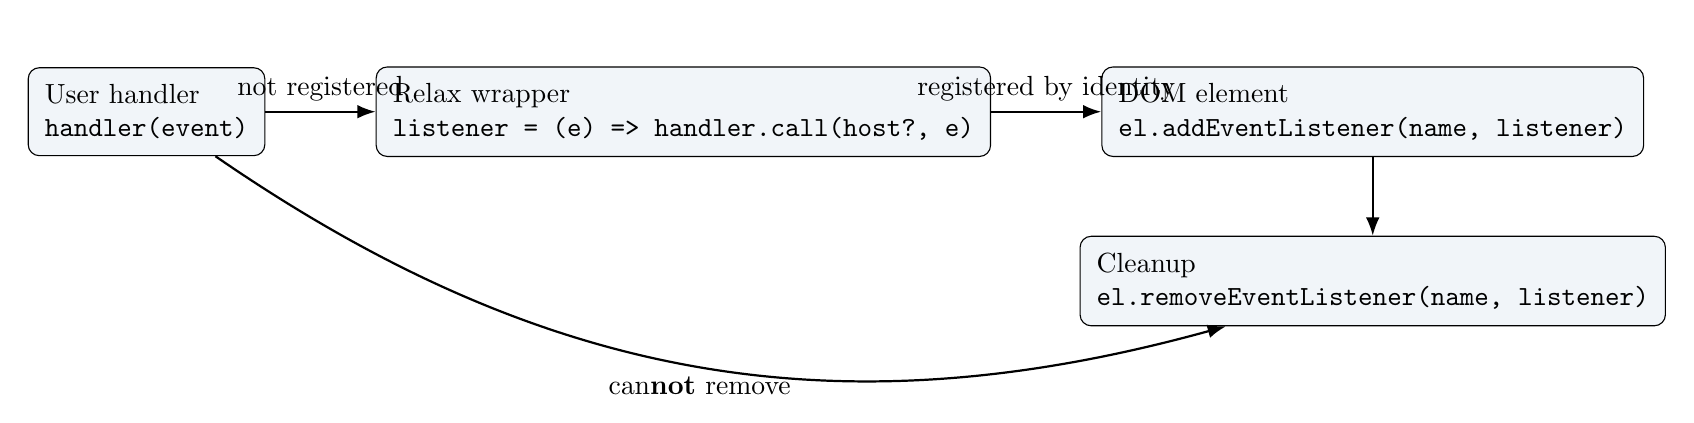
\begin{tikzpicture}[
  node distance=10mm and 14mm,
  box/.style={draw, rounded corners, align=left, inner sep=6pt, fill=RelaxLight},
  arrow/.style={-Latex, thick}
]
\node[box] (user) {User handler\\\texttt{handler(event)}};
\node[box, right=of user] (wrap) {Relax wrapper\\\texttt{listener = (e) => handler.call(host?, e)}};
\node[box, right=of wrap] (dom) {DOM element\\\texttt{el.addEventListener(name, listener)}};

\node[box, below=of dom] (remove) {Cleanup\\\texttt{el.removeEventListener(name, listener)}};

\draw[arrow] (user) -- node[midway, above] {not registered} (wrap);
\draw[arrow] (wrap) -- node[midway, above] {registered by identity} (dom);
\draw[arrow] (dom) -- (remove);

\draw[arrow] (user) to[bend right=25] node[midway, below] {can\textbf{not} remove} (remove);
\end{tikzpicture}
\end{center}

The DOM can only remove listeners by the exact function object identity that was registered. That's why \texttt{events.ts} returns the wrapper.

\section{DOM event listener wiring (\texttt{src/events.ts})}
The central helper is:

\begin{quote}
	exttt{addEventListener(eventName, handler, el, hostComponent?)}
\end{quote}

\subsection{Contract}
\begin{itemize}
  \item \textbf{Inputs:}
    \begin{itemize}
      \item \texttt{eventName}: a DOM event name like \texttt{"click"}.
      \item \texttt{handler}: a function that should run when the event fires.
      \item \texttt{el}: the real DOM element.
      \item \texttt{hostComponent}: optional object used as the \texttt{this} binding.
    \end{itemize}
  \item \textbf{Output:}
    \begin{itemize}
      \item returns the concrete \texttt{listener} function object that was actually registered with \texttt{el.addEventListener}.
    \end{itemize}
\end{itemize}

Returning the registered listener is not a convenience; it's required for correctness.

\subsection{Implementation: the wrapper listener (real code)}
This is the actual implementation from \texttt{src/events.ts}. Notice the wrapper chooses between \texttt{handler.call(hostComponent, event)} and \texttt{handler(event)}:

\begin{lstlisting}[language=JavaScript]
export function addEventListener(
  eventName: string,
  handler: (payload: unknown) => void,
  el: Element,
  hostComponent: any = null
) {
  const listener = (event: Event) => {
    if (hostComponent) {
      handler.call(hostComponent, event)
    } else {
      handler(event)
    }
  }

  el.addEventListener(eventName, listener)
  return listener
}
\end{lstlisting}

This is one of those renderer tricks that's simple but non-negotiable.
If you ever ``refactor'' this into returning \texttt{handler} directly, unmount will leak listeners.

This immediately gives Relax three desirable properties:

\begin{itemize}
  \item \textbf{Stable binding semantics:} the wrapper decides whether to call with \texttt{handler.call(hostComponent, event)}.
  \item \textbf{No mutation of user handlers:} the original function object is untouched.
  \item \textbf{Reliable cleanup:} the wrapper function object can be stored and later removed.
\end{itemize}

\subsection*{Diagram: event wiring lifecycle across mount, patch, destroy}
\begin{center}
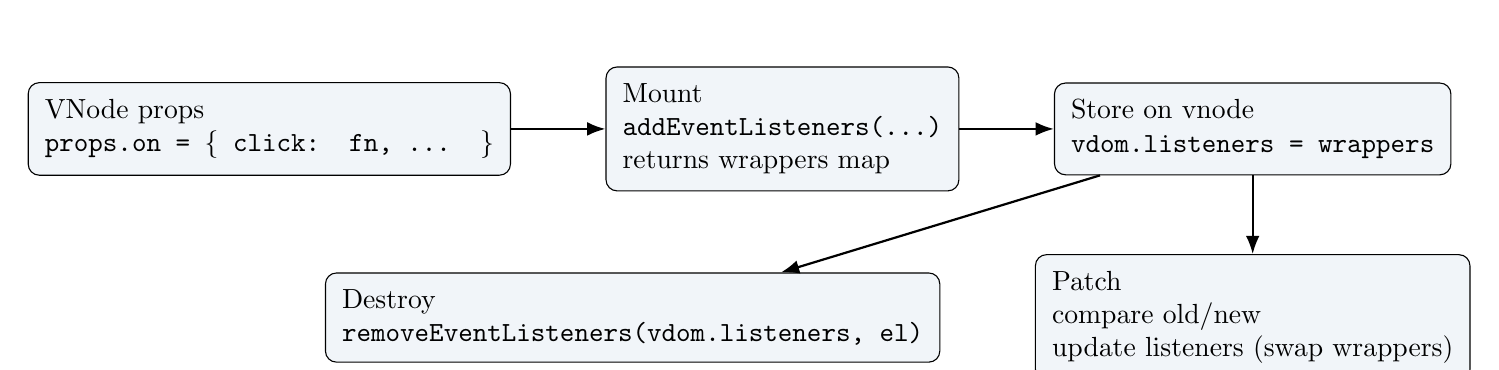
\begin{tikzpicture}[
  node distance=10mm and 12mm,
  box/.style={draw, rounded corners, align=left, inner sep=6pt, fill=RelaxLight},
  arrow/.style={-Latex, thick}
]
\node[box] (props) {VNode props\\\texttt{props.on = \{ click: fn, ... \}}};
\node[box, right=of props] (mount) {Mount\\\texttt{addEventListeners(...)}\\returns wrappers map};
\node[box, right=of mount] (store) {Store on vnode\\\texttt{vdom.listeners = wrappers}};
\node[box, below=of store] (patch) {Patch\\compare old/new\\update listeners (swap wrappers)};
\node[box, left=of patch] (destroy) {Destroy\\\texttt{removeEventListeners(vdom.listeners, el)}};

\draw[arrow] (props) -- (mount);
\draw[arrow] (mount) -- (store);
\draw[arrow] (store) -- (patch);
\draw[arrow] (store) -- (destroy);
\end{tikzpicture}
\end{center}

Even if patch-time logic changes, notice the invariant: destroy always removes \emph{whatever wrappers are currently stored on the vnode}.

\subsection{Multiple listeners: \texttt{addEventListeners(events, el, hostComponent?)}}
Mounting and patching usually deal with an event map (a record of event name to handler). Relax provides a convenience:

\begin{quote}
    exttt{addEventListeners(events, el, hostComponent)}
\end{quote}

Implementation is straightforward:

\begin{itemize}
  \item iterate \texttt{Object.entries(events)}
  \item call \texttt{addEventListener} for each
  \item store returned wrappers in \texttt{listeners: Record<string, EventListener>}
\end{itemize}

The important artifact is the returned \texttt{listeners} map. In \texttt{mount-dom.ts}, Relax stores it on the vnode (\texttt{vdom.listeners}) so that unmounting can remove exactly what was added.

\subsection{Cleanup symmetry: \texttt{removeEventListeners(listeners, el)}}
Removal is the mirror image:

\begin{lstlisting}[language=JavaScript]
Object.entries(listeners).forEach(([eventName, listener]) => {
  el.removeEventListener(eventName, listener)
})
\end{lstlisting}

Note what's \emph{not} present: the original user handlers. Only wrappers can be removed.

\section{Tests for DOM event semantics (\texttt{src/\_\_tests\_\_/events.test.ts})}
The tests are small, but they lock down the two things that tend to regress when you wrap handlers.

\subsection{Invariant 1: wrappers don't break sync or async handlers}
	exttt{events.test.ts} contains:

\begin{itemize}
  \item \texttt{synchronous event without host component, called with argument}
  \item \texttt{asynchronous event without host component}
\end{itemize}

The async test uses \texttt{flushPromises()} (\texttt{src/utils/promises.ts}) after \texttt{btn.click()} to prove that:

\begin{itemize}
  \item the wrapper does not swallow async behavior
  \item the handler is actually invoked and can \texttt{await} microtasks
\end{itemize}

This matters because event wrappers are a common source of subtle bugs where promises aren't awaited or exceptions get lost.

\subsection{Invariant 2: with a host component, \texttt{this} is correct}
Two tests cover binding (sync and async):

\begin{itemize}
  \item \texttt{synchronous event with host component, the handler is bound to component}
  \item \texttt{asynchronous event with host component, the handler is bound to component}
\end{itemize}

Both assert:

\begin{itemize}
  \item \texttt{actualBinding === hostComponent}
  \item the handler argument is an \texttt{Event}
\end{itemize}

If you remember only one idea from this chapter, make it this: \textbf{binding and cleanup are owned by the wrapper function.}

\section{The command dispatcher (\texttt{src/dispatcher.ts})}
Where \texttt{events.ts} is about \emph{browser integration}, \texttt{Dispatcher} is an internal message bus.
I use it for things like devtools hooks, app-level commands, and decoupled communication that doesn't want to bounce through the DOM.

\subsection*{Diagram: dispatcher data structures and dispatch flow}
\begin{center}
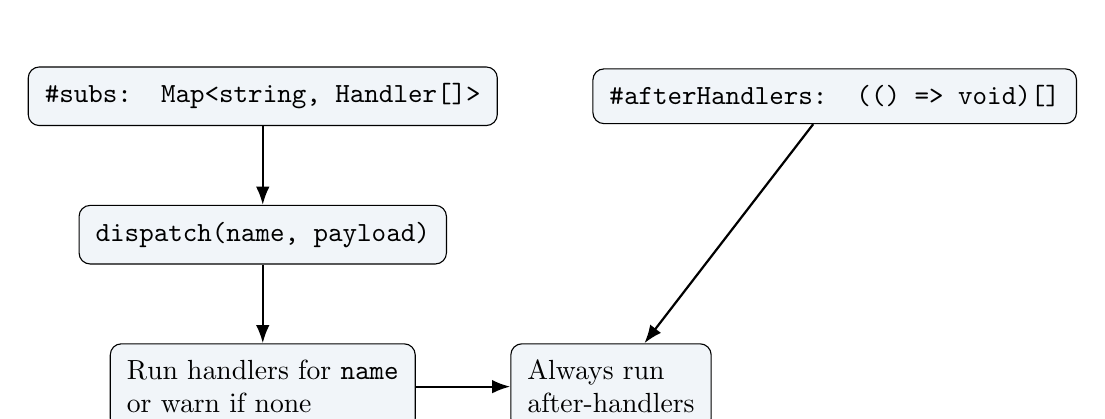
\begin{tikzpicture}[
  node distance=10mm and 12mm,
  box/.style={draw, rounded corners, align=left, inner sep=6pt, fill=RelaxLight},
  arrow/.style={-Latex, thick}
]
\node[box] (subs) {\texttt{\#subs: Map<string, Handler[]>}};
\node[box, right=of subs] (after) {\texttt{\#afterHandlers: (() => void)[]}};
\node[box, below=of subs] (dispatch) {\texttt{dispatch(name, payload)}};
\node[box, below=of dispatch] (handlers) {Run handlers for \texttt{name}\\or warn if none};
\node[box, right=of handlers] (afterRun) {Always run\\after-handlers};

\draw[arrow] (subs) -- (dispatch);
\draw[arrow] (dispatch) -- (handlers);
\draw[arrow] (handlers) -- (afterRun);
\draw[arrow] (after) -- (afterRun);
\end{tikzpicture}
\end{center}

\subsection{A minimal contract}
	exttt{Dispatcher} has three public methods:

\begin{itemize}
  \item \texttt{subscribe(commandName, handler)} \textrightarrow{} returns \texttt{unsubscribe()}
  \item \texttt{afterEveryCommand(handler)} \textrightarrow{} returns \texttt{unsubscribe()}
  \item \texttt{dispatch(commandName, payload)}
\end{itemize}

Internally it stores:

\begin{itemize}
  \item \texttt{\#subs}: \texttt{Map<string, Array<(payload: unknown) => void>>}
  \item \texttt{\#afterHandlers}: \texttt{Array<() => void>}
\end{itemize}

So you can subscribe to a particular command name (payload-aware) and/or attach a hook that runs after every dispatch (payload-agnostic).

\subsection{Subscription semantics: dedupe by function identity}
An important policy choice appears in \texttt{subscribe()}:

\begin{quote}
  registering the same handler function twice is a no-op.
\end{quote}

In code, that's \texttt{handlers.includes(handler)}.

This makes the dispatcher deterministic and prevents accidental handler explosions if a component subscribes in a loop.

\subsection{Dispatch semantics: warn on unhandled commands, always run after-hooks}
	exttt{dispatch(commandName, payload)} does:

\begin{enumerate}
  \item if there are handlers for \texttt{commandName}, call them with \texttt{payload}
  \item otherwise, \texttt{console.warn} (if available): \texttt{No handlers for command: <name>}
  \item always run \texttt{\#afterHandlers}
\end{enumerate}

That last rule is important: after-hooks run even if there were no command handlers.
It allows patterns like global logging, tracing, or devtools hooks.

\section{Tests for dispatcher semantics (\texttt{src/\_\_tests\_\_/dispatcher.test.ts})}
The dispatcher tests are a clean, readable spec for the API:

\begin{itemize}
  \item \textbf{subscribe/unsubscribe works:} the handler is called once, then not called after unsubscribe.
  \item \textbf{dedupe works:} subscribing the same handler multiple times still results in one call per dispatch.
  \item \textbf{multiple handlers work:} two different handlers both fire, and both can unsubscribe.
  \item \textbf{afterEveryCommand works:} runs once per dispatch and unsubscribes cleanly.
\end{itemize}

Notice how these tests avoid implementation details (maps, arrays, indices) and instead assert the observable contract.

\section{Common pitfalls and edges}
\begin{itemize}
  \item \textbf{Listener removal requires wrapper identity.} Never attempt to remove a handler by passing the original user function if you registered a wrapper.
  \item \textbf{Dedupe is per-function identity.} If you pass a new \texttt{() => ...} lambda each time, the dispatcher will treat it as a different handler.
  \item \textbf{Dispatcher is synchronous.} If a handler throws, that throw will propagate from \texttt{dispatch()}.
\end{itemize}

\section{Mini-exercises}
\begin{enumerate}
  \item In \texttt{src/events.ts}, add a new helper \texttt{updateEventListeners(old, next, el, hostComponent)} that returns the new wrappers map without leaking old listeners. (Don't implement it here; design the contract and write the tests first.)
  \item Extend \texttt{dispatcher.test.ts} with a test that proves after-handlers run even when there are \emph{no} command handlers for a dispatch.
  \item Thought exercise: should \texttt{Dispatcher.subscribe()} remove the command entry from \texttt{\#subs} when the last handler unsubscribes? What trade-offs does that create?
\end{enumerate}

\section{Where this plugs into the renderer}
You've already seen the integration point in Chapter~\ref{ch:mounting}:

\begin{itemize}
  \item element vnodes store \texttt{props.on} (after TSX mapping)
  \item mounting calls \texttt{addEventListeners(...)} and saves wrapper functions on \texttt{vdom.listeners}
  \item destroying later calls \texttt{removeEventListeners(vdom.listeners, el)}
\end{itemize}

The remaining questions, how listeners are updated during patch without leaking, and how host binding is preserved across updates, live in \texttt{src/patch-dom.ts} and \texttt{src/destroy-dom.ts}.

\section{Online resources}
\begin{itemize}
  \item DOM events and bubbling (MDN): \href{https://developer.mozilla.org/en-US/docs/Learn_web_development/Core/Scripting/Event_bubbling}{\url{https://developer.mozilla.org/en-US/docs/Learn_web_development/Core/Scripting/Event_bubbling}}
  \item \texttt{EventTarget.addEventListener} / \texttt{removeEventListener} (MDN): \href{https://developer.mozilla.org/en-US/docs/Web/API/EventTarget/addEventListener}{\url{https://developer.mozilla.org/en-US/docs/Web/API/EventTarget/addEventListener}}
  \item Function \texttt{call} and \texttt{this} binding (MDN): \href{https://developer.mozilla.org/en-US/docs/Web/JavaScript/Reference/Global_Objects/Function/call}{\url{https://developer.mozilla.org/en-US/docs/Web/JavaScript/Reference/Global_Objects/Function/call}}
  \item Message bus / pub-sub as a pattern (Wikipedia overview): \href{https://en.wikipedia.org/wiki/Publish%E2%80%93subscribe_pattern}{\url{https://en.wikipedia.org/wiki/Publish-subscribe_pattern}}
\end{itemize}

\chapter{Patching and Diffing: Updating the DOM Efficiently}

Mounting is the ``first render'' story. But real apps are dominated by \emph{updates}: state changes, input events, list reorders, and component re-renders.

Relax's patcher has one job: given an \emph{old} VNode tree that is already mounted and a \emph{new} VNode tree produced by the latest render, mutate the real DOM so it matches the new tree while reusing as much existing DOM as is safe.

In Relax the patcher is both:

\begin{itemize}
  \item \textbf{small enough to read end-to-end} (in \texttt{src/patch-dom.ts}), and
  \item \textbf{heavily specified by tests} (especially \texttt{src/\_\_tests\_\_/patch-dom.test.ts}).
\end{itemize}

This chapter is long because patching is where most correctness and performance edge cases live.

\section{Diagram: the patch decision tree}
Before reading any helper functions, keep this diagram in mind. It summarizes the control flow inside \texttt{patchDOM}:

\begin{center}
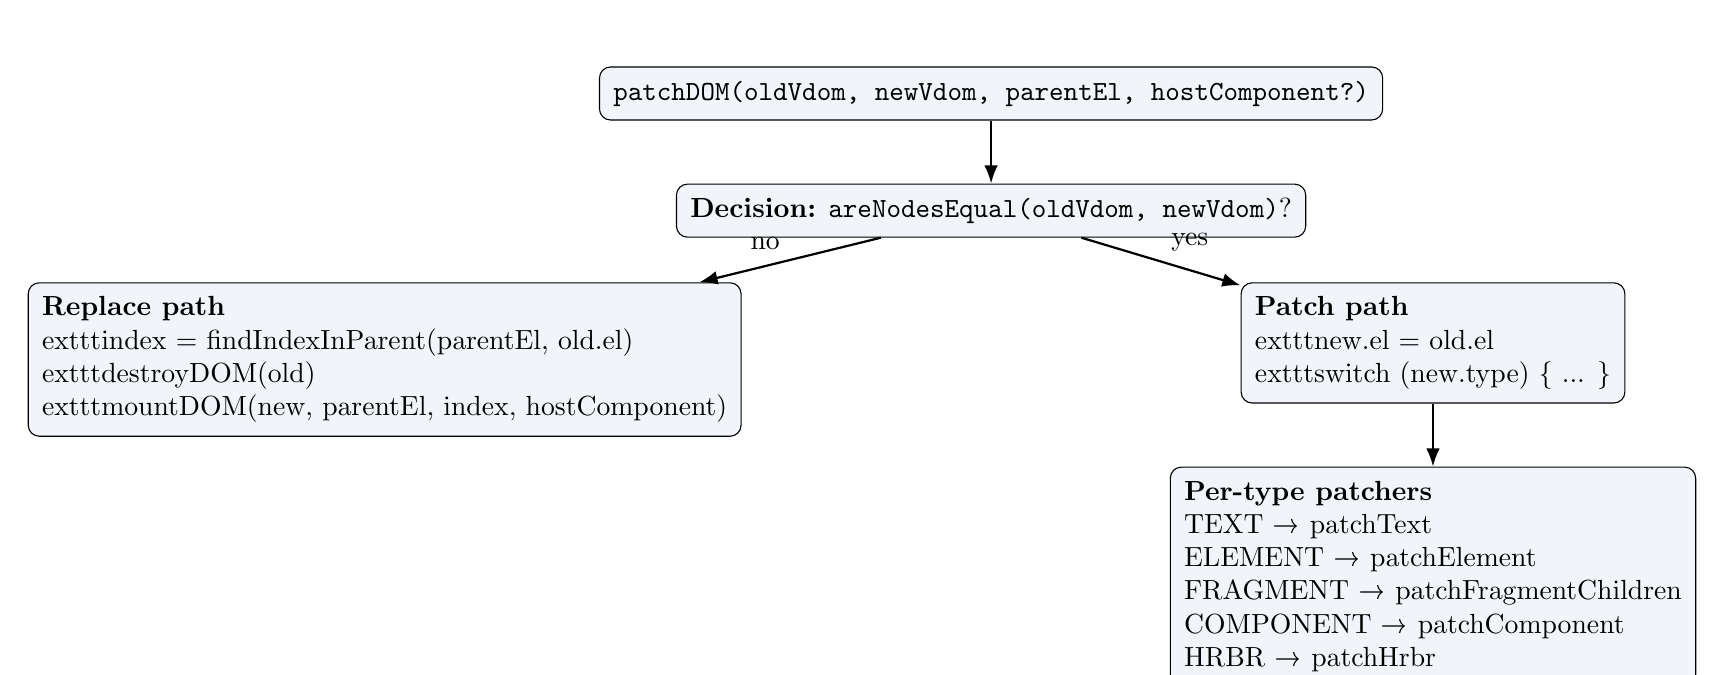
\begin{tikzpicture}[
  node distance=8mm,
  box/.style={draw,rounded corners,fill=RelaxLight,inner sep=5pt,align=left},
  arrow/.style={-Latex,thick}
]
  \node[box] (start) {\texttt{patchDOM(oldVdom, newVdom, parentEl, hostComponent?)}};
  \node[box, below=of start] (eq) {\textbf{Decision:} \texttt{areNodesEqual(oldVdom, newVdom)}?};

  \node[box, below left=of eq, xshift=14mm] (replace) {\textbf{Replace path}\\
  	exttt{index = findIndexInParent(parentEl, old.el)}\\
  	exttt{destroyDOM(old)}\\
  	exttt{mountDOM(new, parentEl, index, hostComponent)}};

  \node[box, below right=of eq, xshift=-14mm] (patch) {\textbf{Patch path}\\
  	exttt{new.el = old.el}\\
  	exttt{switch (new.type) \{ ... \}}};

  \node[box, below=of patch] (dispatch) {\textbf{Per-type patchers}\\
  TEXT \textrightarrow{} patchText\\
  ELEMENT \textrightarrow{} patchElement\\
  FRAGMENT \textrightarrow{} patchFragmentChildren\\
  COMPONENT \textrightarrow{} patchComponent\\
  HRBR \textrightarrow{} patchHrbr};

  \draw[arrow] (start) -- (eq);
  \draw[arrow] (eq) -- node[above left]{no} (replace);
  \draw[arrow] (eq) -- node[above right]{yes} (patch);
  \draw[arrow] (patch) -- (dispatch);
\end{tikzpicture}
\end{center}

This picture also explains why Chapter~4's invariant (children are always VNodes) matters: it makes the \texttt{switch} and its helper patchers tractable.

\section{\texttt{patchDOM}: the top-level operation}
The public entry point is:

\begin{quote}
    exttt{patchDOM(oldVdom, newVdom, parentEl, hostComponent?)}
\end{quote}

It lives in \texttt{src/patch-dom.ts}.

\subsection{Contract}

\begin{itemize}
  \item \textbf{Inputs}
    \begin{itemize}
      \item \texttt{oldVdom}: the currently mounted VNode tree.
      \item \texttt{newVdom}: the VNode tree produced by the latest render.
      \item \texttt{parentEl}: the DOM parent that contains \texttt{oldVdom.el}.
      \item \texttt{hostComponent}: optional component instance used to bind events and to account for fragment offsets.
    \end{itemize}
  \item \textbf{Output}
    \begin{itemize}
      \item Returns the patched \texttt{newVdom} (with \texttt{newVdom.el} pointing at the reused DOM).
    \end{itemize}
  \item \textbf{Key invariant}
    \begin{itemize}
      \item After patching, the returned tree (the \emph{new} VDOM) must contain correct \texttt{.el} references.
    \end{itemize}
\end{itemize}

\subsection{Replace vs patch: areNodesEqual}

The first decision is whether two nodes are ``the same'' (so we can patch in place) or different (so we must replace).

Relax defines ``same'' in \texttt{src/nodes-equal.ts} via \texttt{areNodesEqual(oldNode, newNode)}.

This is not a philosophical definition of equality; it is \emph{exactly} the predicate the patcher uses to decide between:

\begin{itemize}
  \item patching in place (reuse), or
  \item destroying and remounting (replace).
\end{itemize}

The current identity rules are:

\begin{itemize}
  \item If \texttt{type} differs: not equal.
  \item \textbf{TEXT}: always equal (text nodes are patched by content).
  \item \textbf{ELEMENT}: equal when \texttt{tag} matches and \texttt{key} matches.
  \item \textbf{COMPONENT}: equal when component function identity (\texttt{tag}) matches and \texttt{key} matches.
  \item \textbf{HRBR}: equal when \texttt{mount} factory identity matches.
\end{itemize}

\paragraph{Why identity is intentionally strict}
Virtual DOM patching is always a trade-off between reuse and correctness. Relax chooses a conservative identity rule:

\begin{itemize}
  \item If identity says "not equal", Relax pays the cost of teardown + remount.
  \item The upside is that "equal" becomes a promise: the patcher can safely assume the DOM node kind matches what it needs to mutate.
\end{itemize}

In other words, \texttt{areNodesEqual} isn't about "deep equality". It's a \emph{safety gate} that defends the patcher.

\paragraph{A renderer mental model: identity answers ``can I mutate in place?''}
When I say two VNodes are ``equal'' in Relax, I don't mean their props match.
I mean something narrower and more operational:

\begin{quote}
If I keep the existing DOM node, do I still have the right \emph{kind} of DOM node to mutate into the new node?
\end{quote}

That’s why:

\begin{itemize}
  \item TEXT nodes are always patchable (you can always update \texttt{nodeValue}).
  \item ELEMENT nodes require the same \texttt{tag} and the same \texttt{key}.
  \item COMPONENT nodes require the same component function identity (\texttt{tag}) and the same \texttt{key}.
\end{itemize}

That strictness is what keeps the rest of the patcher simple.
When identity says ``yes'', every per-type patch function can assume it's operating on the right DOM shape.

If nodes are not equal, \texttt{patchDOM} does a replacement:

\begin{enumerate}
  \item Find the current DOM index of \texttt{oldVdom.el} inside \texttt{parentEl} (\texttt{findIndexInParent}).
  \item Destroy the old subtree (\texttt{destroyDOM(oldVdom)}).
  \item Mount the new subtree at the same index (\texttt{mountDOM(newVdom, parentEl, index, hostComponent)}).
\end{enumerate}

This behavior is covered early in \texttt{src/\_\_tests\_\_/patch-dom.test.ts} by:

\begin{itemize}
  \item \texttt{change the root node}
  \item \texttt{change the root node, mount in same index}
\end{itemize}

\subsection{When nodes are equal: preserve el}

If nodes are equal, patching starts by reusing the DOM reference:

\begin{lstlisting}[language=JavaScript]
newVdom.el = oldVdom.el
\end{lstlisting}

This is asserted by tests like \texttt{no change} and \texttt{sets the el in the new vdom}.

\section{Node-type specific patching}

After equality is established, patching dispatches on \texttt{newVdom.type} (see \texttt{DOM\_TYPES} in \texttt{src/h.ts}).

\subsection{Text nodes: patchText}

\texttt{patchText(oldVdom, newVdom)} compares \texttt{oldVdom.value} and \texttt{newVdom.value}. If different, it updates \texttt{Text.nodeValue}.

Test: \texttt{patch text}.

\subsection{Element nodes: patchElement}

\texttt{patchElement(oldVdom, newVdom, hostComponent)} updates four categories of props:

\begin{itemize}
  \item Attributes/properties (everything except \texttt{class}, \texttt{style}, \texttt{on})
  \item \texttt{class}
  \item \texttt{style}
  \item \texttt{on} (DOM event handlers)
\end{itemize}

Implementation detail: it destructures props like:

\begin{lstlisting}[language=JavaScript]
const { class: oldClass, style: oldStyle, on: oldEvents, ...oldAttrs } = oldVdom.props
const { class: newClass, style: newStyle, on: newEvents, ...newAttrs } = newVdom.props
\end{lstlisting}

and then applies targeted patchers:

\begin{itemize}
  \item \texttt{patchAttrs(el, oldAttrs, newAttrs)}
  \item \texttt{patchClasses(el, oldClass, newClass)}
  \item \texttt{patchStyles(el, oldStyle, newStyle)}
  \item \texttt{patchEvents(el, oldListeners, oldEvents, newEvents, hostComponent)}
\end{itemize}

\paragraph{Micro-optimization: object identity fast paths}

Notice the checks in \texttt{patchElement}:

\begin{verbatim}
if (oldAttrs !== newAttrs) { ... }
if (oldClass !== newClass) { ... }
if (oldStyle !== newStyle) { ... }
\end{verbatim}

In large lists, applications often reuse the same props objects (or stable sub-objects) for unchanged rows.
These identity checks avoid unnecessary diff work.

\subsection{Attributes: patchAttrs uses objectsDiff}

\texttt{patchAttrs} calls \texttt{objectsDiff(oldAttrs, newAttrs)} (from \texttt{src/utils/objects.ts}) to compute \texttt{added}, \texttt{removed}, \texttt{updated}.

It then:

\begin{itemize}
  \item removes: \texttt{removeAttribute(el, name)}
  \item adds/updates: \texttt{setAttribute(el, name, value)}
\end{itemize}

Important: \texttt{setAttribute} and \texttt{removeAttribute} are the same helpers discussed in Chapter 6 (\texttt{src/attributes.ts}), including the property-vs-attribute rules.

\subsection{Classes: patchClasses uses arraysDiff}

\texttt{patchClasses} normalizes both old and new values into an array of class tokens using \texttt{toClassList}.

Then it runs \texttt{arraysDiff(oldClasses, newClasses)} to compute \texttt{added} and \texttt{removed}, and performs:

\begin{itemize}
  \item \texttt{el.classList.remove(...removed)}
  \item \texttt{el.classList.add(...added)}
\end{itemize}

The behavior is tested extensively in \texttt{patch class} cases in \texttt{src/\_\_tests\_\_/patch-dom.test.ts}.

\subsection{Styles: patchStyles uses objectsDiff}

\texttt{patchStyles} again uses \texttt{objectsDiff} and applies:

\begin{itemize}
  \item remove: \texttt{removeStyle(el, key)}
  \item add/update: \texttt{setStyle(el, key, value)}
\end{itemize}

Test group: \texttt{patch style}.

\subsection{Events: patchEvents}

\texttt{patchEvents} compares old and new \texttt{on} objects using \texttt{objectsDiff} and performs two phases:

\begin{enumerate}
  \item \textbf{Detach} removed and updated handlers by removing their old wrapper listeners.
  \item \textbf{Attach} added and updated handlers using \texttt{addEventListener} from \texttt{src/events.ts}.
\end{enumerate}

Why detach+attach for \emph{updated}?
Because the wrapper listener function identity changes when the handler changes.

\paragraph{Why this detail matters so much}
When people build their first patcher, they often try to "update" an event handler by doing nothing:
``the new handler is different, but the event name is the same, so surely the browser will call the new one.''

That doesn't work.
In the DOM, \texttt{addEventListener} doesn't register "an event called click".
It registers a \emph{pair}: \texttt{(eventName, functionObject)}.
Removal uses the same pair.

Relax solves this with the wrapper identity trick from Chapter~7, and the patcher follows the same rule:

\begin{itemize}
  \item if a handler is removed or updated, remove the old wrapper function
  \item if a handler is added or updated, add a fresh wrapper function
  \item store the wrapper map on the vnode (\texttt{vdom.listeners}) so destroy can remove correctly
\end{itemize}

If you look at the real implementation in \texttt{src/patch-dom.ts}, the important part is the ordering:
we remove first, then add. That prevents accidental double-binding during an update.

\paragraph{Diagram: event patching as identity management}
This is the subtle part: the browser removes listeners by the \emph{exact function object} you originally passed.

\begin{center}
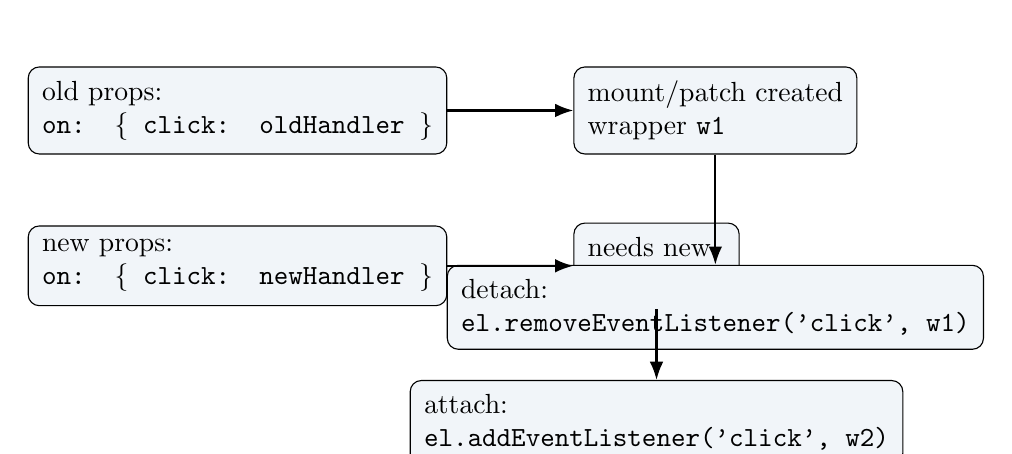
\begin{tikzpicture}[
  node distance=9mm,
  box/.style={draw,rounded corners,fill=RelaxLight,inner sep=5pt,align=left},
  arrow/.style={-Latex,thick}
]
  \node[box] (old) {old props:\\\texttt{on: \{ click: oldHandler \}}};
  \node[box, right=16mm of old] (wrap1) {mount/patch created\\wrapper \texttt{w1}};
  \node[box, below=of old] (new) {new props:\\\texttt{on: \{ click: newHandler \}}};
  \node[box, right=16mm of new] (wrap2) {needs new\\wrapper \texttt{w2}};

  \node[box, below=14mm of wrap1] (detach) {detach:\\\texttt{el.removeEventListener('click', w1)}};
  \node[box, below=of wrap2] (attach) {attach:\\\texttt{el.addEventListener('click', w2)}};

  \draw[arrow] (old) -- (wrap1);
  \draw[arrow] (new) -- (wrap2);
  \draw[arrow] (wrap1) -- (detach);
  \draw[arrow] (wrap2) -- (attach);
\end{tikzpicture}
\end{center}

Tests like \texttt{patch event handlers} effectively specify this: "updating" a handler is implemented as remove+add because the wrapper identity changes.

Tests to read:

\begin{itemize}
  \item \texttt{patch event handlers} in \texttt{src/\_\_tests\_\_/patch-dom.test.ts}
  \item The binding rules in \texttt{src/\_\_tests\_\_/events.test.ts}
\end{itemize}

\subsection{Component nodes: patchComponent}

\texttt{patchComponent(oldVdom, newVdom)} preserves the component instance and pushes changes into it.

Key steps:

\begin{itemize}
  \item Extract external children and props (see \texttt{extractPropsAndEvents} in \texttt{src/utils/props.ts}).
  \item Call \texttt{component.setExternalContent(children)}.
  \item Call \texttt{component.updateProps(props)}.
  \item Copy instance fields:
    \begin{itemize}
      \item \texttt{newVdom.component = component}
      \item \texttt{newVdom.el = component.firstElement}
    \end{itemize}
\end{itemize}

This is how Relax achieves the "component instance is preserved" semantics tested in \texttt{patch component with props}.

\subsection{HRBR nodes: patchHrbr}

\subsection{A tiny but important helper: \texttt{patchDOMSameElement}}
You will notice a second patch entry point inside \texttt{src/patch-dom.ts}:

\begin{quote}
    exttt{patchDOMSameElement(oldVdom, newVdom, hostComponent?)}
\end{quote}

It is identical to \texttt{patchDOM} except it \emph{skips the replacement path} and therefore does not need \texttt{parentEl}.

This helper is used in child diffing paths where:

\begin{itemize}
  \item we already know the node should be kept (for example, keyed nodes that exist in both old and new), and
  \item we want to avoid scanning \texttt{parentEl.childNodes} to find the current index for every child.
\end{itemize}

When you're reading patching code, seeing \texttt{patchDOMSameElement} is a clue: ``we're in an optimization path, and we've already committed to reusing the node identity.''

Relax contains an experimental HRBR interop mode. In \texttt{patch-dom.ts}, \texttt{patchHrbr(old, next)}:

\begin{itemize}
  \item Reuses the existing mounted instance when \texttt{old.mount === next.mount}.
  \item Otherwise, disposes/destroys the old instance and remounts into the same host element.
\end{itemize}

This behavior matches the spec tests in \texttt{src/\_\_tests\_\_/hrbr-integration.test.ts}.

\section{Patching children: from fast paths to general diff}

After patching the node itself, Relax patches children with:

\begin{lstlisting}[language=JavaScript]
patchChildren(oldVdom, newVdom, hostComponent)
\end{lstlisting}

This is where most performance work lives, and \texttt{src/patch-dom.ts} contains several layered strategies.

\subsection{Step 0: child extraction}

Children are normalized by \texttt{extractChildren(oldVdom)} / \texttt{extractChildren(newVdom)} from \texttt{src/h.ts}.
This lets fragments and components present children uniformly.

\subsection{Fast path A (opt-in): delegate keyed list reconciliation to HRBR reconciler}

There is an optional integration with the runtime reconciler:

\begin{verbatim}
if (newVdom.props.\_reconcile === 'hrbr') { ... reconcileChildren(...) }
\end{verbatim}

This path only applies when \emph{all direct children are keyed} (keyed list). It builds \texttt{ReconcileNode} specs and lets \texttt{reconcileChildren} (from \texttt{runtime/reconciler}) patch/move nodes with a single keyed pass.

You can think of it as: "VDOM delegates list diffing to a specialized keyed reconciler".

\subsection{Fast path B (opt-in): \_textOnly rows}

For large lists of rows shaped like \texttt{<li>{label}</li>}, Relax supports an opt-in hint:

\begin{itemize}
  \item If \texttt{oldVdom.props.\_textOnly === true} and \texttt{newVdom.props.\_textOnly === true}, and
  \item both old and new children are exactly one TEXT node,
\end{itemize}

then patchChildren patches only the text node via \texttt{patchDOMSameElement}.

Test name: \texttt{patchChildren row fast path (\_textOnly)}.

\subsection{Fast path C: keyed reorder via LIS}

The LIS (Longest Increasing Subsequence) trick is a classic VDOM strategy:

\begin{itemize}
  \item If you can identify the subsequence of children that are already in correct relative order,
  \item then you only need to move the remaining nodes.
\end{itemize}

Relax's implementation is in \texttt{patchKeyedChildrenReorder(...)} and uses an internal helper \texttt{lisIndices(arr)} which computes LIS indices over a sequence of old positions (ignoring \texttt{-1} markers for new nodes).

One very practical detail from the code: \texttt{elementsForChild(child)} returns \emph{multiple} DOM elements for components (using \texttt{child.component.elements}) but only one for normal elements. That's how the reorder path correctly moves a component that renders multiple siblings.

\texttt{patchKeyedChildrenReorder(oldChildren, newChildren, parentEl, hostComponent)} implements keyed reordering with minimal DOM moves:

\begin{enumerate}
  \item Ensure both sides are fully keyed.
  \item Remove old nodes not present in the new key set.
  \item Patch existing nodes and mark new nodes with \texttt{-1} in a sequence.
  \item Compute the Longest Increasing Subsequence (LIS) over old indices.
  \item Walk backwards, mounting new nodes and moving only nodes not in LIS.
\end{enumerate}

This is a classic strategy: nodes in the LIS are already in relative order, so moving the rest yields the fewest inserts/reorders.

\subsubsection*{Diagram: keyed children reconciliation with LIS}
This is the bird's-eye view of what \texttt{patchKeyedChildrenReorder} is doing:

\begin{center}
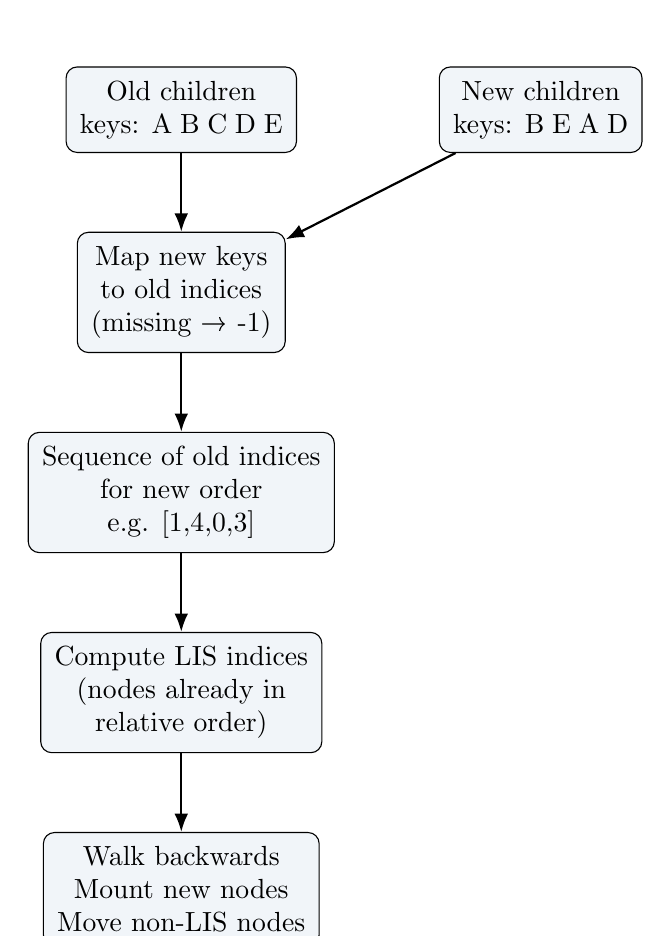
\begin{tikzpicture}[
  node distance=10mm,
  box/.style={draw,rounded corners,fill=RelaxLight,inner sep=5pt,align=center},
  arrow/.style={-Latex,thick}
]
  \node[box] (old) {Old children\\keys: A\;B\;C\;D\;E};
  \node[box, right=18mm of old] (new) {New children\\keys: B\;E\;A\;D};

  \node[box, below=of old] (map) {Map new keys\\to old indices\\(missing \textrightarrow{} -1)};
  \node[box, below=of map] (seq) {Sequence of old indices\\for new order\\e.g. [1,4,0,3]};
  \node[box, below=of seq] (lis) {Compute LIS indices\\(nodes already in\\relative order)};
  \node[box, below=of lis] (walk) {Walk backwards\\Mount new nodes\\Move non-LIS nodes};

  \draw[arrow] (old) -- (map);
  \draw[arrow] (new) -- (map);
  \draw[arrow] (map) -- (seq);
  \draw[arrow] (seq) -- (lis);
  \draw[arrow] (lis) -- (walk);
\end{tikzpicture}
\end{center}

The reason for the backward walk is practical DOM surgery: when you insert/move nodes from the end, you don't invalidate the insertion positions you haven't processed yet.

Test names to read:

\begin{itemize}
  \item \texttt{patchChildren keyed reorder fast path (LIS)}
  \item The many keyed reorder cases in \texttt{src/\_\_tests\_\_/patch-dom.test.ts}
\end{itemize}

\subsection{Fast path D: stable keyed same-order}

If keys are present and the order is identical, Relax avoids diff work entirely:

\begin{verbatim}
if (isStableKeyedSameOrder(oldChildren, newChildren)) {
  for (i) patchDOMSameElement(oldChildren[i], newChildren[i])
  return
}
\end{verbatim}

Test name: \texttt{patchChildren fast path (stable keyed order)}.

\subsection{General path: arraysDiffSequence}

If none of the fast paths apply, Relax computes an edit script:

\begin{verbatim}
const diffSeq = arraysDiffSequence(oldChildren, newChildren, areNodesEqual)
\end{verbatim}



	exttt{arraysDiffSequence} is a general-purpose utility in \texttt{src/utils/arrays.ts}. It's worth reading because it is one of the algorithmic cores of Relax.

It has extensive unit tests in:

\begin{itemize}
  \item \texttt{src/\_\_tests\_\_/diff-sequence.test.ts}
  \item \texttt{src/\_\_tests\_\_/diff-sequence.fuzzy.test.ts}
\end{itemize}

It produces operations of types \texttt{ADD}, \texttt{REMOVE}, \texttt{MOVE}, \texttt{NOOP} (see \texttt{ARRAY\_DIFF\_OP}).

\subsubsection*{How to read the diff algorithm (from scratch)}


	exttt{arraysDiffSequence(oldArr, newArr, equals)} returns an \emph{edit script}.
An edit script is just a list of operations that, when applied left-to-right, transforms \texttt{oldArr} into \texttt{newArr}.

Relax's implementation in \texttt{src/utils/arrays.ts} is practical, not academic:

\begin{itemize}
  \item It walks \texttt{newArr} from left to right.
  \item At each index it decides whether the current old item must be removed, can stay (NOOP), needs to be added (ADD), or needs to be moved (MOVE).
  \item It tracks \emph{original indices} so tests can assert stable semantics even as the working array mutates.
\end{itemize}

This is exactly the kind of algorithm that's easy to get "mostly working" and still be wrong in edge cases.
That's why Relax has both:

\begin{itemize}
  \item exact expected sequences in \texttt{diff-sequence.test.ts}, and
  \item randomized fuzz tests in \texttt{diff-sequence.fuzzy.test.ts}.
\end{itemize}

I recommend reading one fuzzy test before you touch the diff logic.
It teaches you what you're \emph{actually} allowed to change.

Then \texttt{patchChildren} executes them:

\begin{itemize}
  \item \textbf{ADD}: \texttt{mountDOM(item, parentEl, index + offset, hostComponent)}
  \item \textbf{REMOVE}: \texttt{destroyDOM(item)}
  \item \textbf{MOVE}: move DOM nodes (component = multiple elements) and patch the moved subtree
  \item \textbf{NOOP}: patch the subtree in place
\end{itemize}

\subsubsection*{How Relax executes the edit script (the part people usually hand-wave)}

This is the section that makes the whole chapter ``click''.

At this point we have:

\begin{itemize}
  \item a concrete \texttt{parentEl} (the real DOM element we will mutate),
  \item \texttt{oldChildren} (already mounted; each node has \texttt{.el} pointers),
  \item \texttt{newChildren} (fresh objects from render; \texttt{.el} mostly unset), and
  \item \texttt{diffSeq}, a list of ops that converts old \textrightarrow{} new.
\end{itemize}

The important subtlety is this: \textbf{the DOM has one truthy linear order, but our algorithm temporarily has two competing linear orders}.
As we apply operations, \texttt{oldChildren} is being mutated (conceptually) and the DOM is being mutated (physically).
That is why \texttt{patchChildren} needs an \texttt{offset}.

\paragraph{What is \texttt{offset}?}

Think of \texttt{index} in the edit script as an index in the \emph{new} children list.
But when we insert or remove DOM nodes, the ``current DOM index we should insert at'' shifts relative to that new index.

Relax models that shift with:

\begin{itemize}
  \item \texttt{offset += 1} when it mounts an item (the DOM got longer than the old list),
  \item \texttt{offset -= 1} when it destroys an item (the DOM got shorter than the old list).
\end{itemize}

So the effective DOM insertion index becomes \texttt{index + offset}.

\subsubsection*{Operation semantics in detail}

Below is a readable version of what the real code is doing (names simplified; still faithful to intent):

\begin{lstlisting}[language=JavaScript]
let offset = 0

for (const op of diffSeq) {
  const { type, index, item, from } = op

  if (type === 'ADD') {
    // Insert a brand-new subtree.
    mountDOM(item, parentEl, index + offset, hostComponent)
    offset += 1
    continue
  }

  if (type === 'REMOVE') {
    // Tear down a mounted subtree (also unbinds events).
    destroyDOM(item)
    offset -= 1
    continue
  }

  if (type === 'MOVE') {
    // 1) Move DOM nodes to the new position
    // 2) Then patch the subtree in place (so props/events update)
    // (MOVE is not just reorder; it implies we still need to patch.)
    const oldChild = oldChildren[from]
    const newChild = item

    moveDomForVNode(oldChild, parentEl, index + offset)
    patchDOMSameElement(oldChild, newChild, hostComponent)
    continue
  }

  // NOOP: same identity at this position, but props may differ.
  patchDOMSameElement(item.old, item.new, hostComponent)
}
\end{lstlisting}

This is also why Relax is strict about \texttt{areNodesEqual}: if a node is ``equal'', we assume we can move/patch it without changing its fundamental DOM shape.

\paragraph{MOVE for components (multi-element reality)}

Moving an \emph{element vnode} means moving one DOM element.
Moving a \emph{component vnode} often means moving \textbf{multiple} DOM siblings, because a component can render "fragment-like" output.

That is why the implementation builds the move list like:

\begin{lstlisting}[language=JavaScript]
const elementsToMove = isComponent(oldChild)
  ? oldChild.component.elements
  : [oldChild.el]
\end{lstlisting}

Then it inserts each element in order at the target position.
If you only moved \texttt{component.firstElement} and forgot the rest, you'd silently corrupt the DOM order.

\subsubsection*{A concrete mental simulation}

Here is a small sequence you can replay by hand:

\begin{itemize}
  \item old keys: \texttt{[A, B, C]}
  \item new keys: \texttt{[B, D, A]}
\end{itemize}

A sensible edit script is:

\begin{itemize}
  \item MOVE \texttt{B} to index 0
  \item ADD \texttt{D} at index 1
  \item MOVE \texttt{A} to index 2
  \item REMOVE \texttt{C}
\end{itemize}

As soon as \texttt{D} is added, the DOM becomes longer than the original, so the correct target indices for later operations must account for that. That's exactly what \texttt{offset} encodes.

\subsection{What the patch-children tests specify (without running them)}

The tests in \texttt{src/\_\_tests\_\_/patch-dom.test.ts} are effectively a spec for these semantics. In particular, they lock down:

\begin{itemize}
  \item \textbf{No-op patching still updates}: even when the vnode identity matches, prop diffs still apply.
  \item \textbf{Moves preserve identity but update content}: moved nodes keep their DOM element(s), but still get patched.
  \item \textbf{Component move moves all owned elements}: multi-element components reorder correctly.
  \item \textbf{Index stability}: when replacing the root, new nodes mount into the same parent index.
\end{itemize}

If you ever change \texttt{patchChildren}, read those tests first. They tell you what behavior is intentional and what behavior would be a breaking change.

\paragraph{Component moves}

A subtle point: moving a component means moving \emph{all} DOM elements owned by that component.
That’s why the code does:

\begin{verbatim}
const elementsToMove = isComponent(oldChild)
  ? oldChild.component.elements
  : [oldChild.el]
\end{verbatim}

This matches the ``component as a fragment'' mental model: the component is a logical node that may span multiple DOM siblings.

\subsection{What the diff-sequence tests prove}
The patcher relies on \texttt{arraysDiffSequence} to produce a valid edit script. The contract is captured in two test files:

\begin{itemize}
  \item \texttt{src/\_\_tests\_\_/diff-sequence.test.ts}: a human-readable set of exact expected operation sequences for many small cases
  \item \texttt{src/\_\_tests\_\_/diff-sequence.fuzzy.test.ts}: a property-style test that generates random arrays and asserts that applying the operations reproduces the target array
\end{itemize}

The workhorse assertion is essentially:

\begin{quote}
    exttt{applyArraysDiffSequence(oldArray, arraysDiffSequence(oldArray, newArray)) === newArray}
\end{quote}

This is a great example of how Relax uses tests: not just to assert a single result, but to lock down the correctness of an algorithm under many variations.

\section{Tests to lean on}

If you want to understand Relax patch semantics quickly, scan these groups in \texttt{src/\_\_tests\_\_/patch-dom.test.ts}:

\begin{itemize}
  \item Root replacement and \texttt{.el} preservation.
  \item Fragment patching (nested add/remove/move).
  \item Attribute/class/style patching.
  \item Event handler updates and removals.
  \item Children patching: keyed/unkeyed, moves, fast paths.
  \item Component patching and component list semantics.
\end{itemize}

\section{Takeaways}

\begin{itemize}
  \item Relax’s patcher is layered: correct general diff + several pragmatic fast paths for real-world performance.
  \item Keys are not just an optimization; they unlock better move semantics and fewer DOM operations.
  \item Correctness depends on two invariants:
    \begin{itemize}
      \item \texttt{areNodesEqual} must be consistent across mount/patch.
      \item \texttt{newVdom.el} (and component element arrays) must be updated to reflect reality.
    \end{itemize}
\end{itemize}

\section{Online resources}
\begin{itemize}
  \item React keys and list rendering (conceptual background; implementation differs): \href{https://react.dev/learn/rendering-lists}{https://react.dev/learn/rendering-lists}
  \item Longest Increasing Subsequence (LIS) algorithm overview: \href{https://en.wikipedia.org/wiki/Longest\_increasing\_subsequence}{https://en.wikipedia.org/wiki/Longest\_increasing\_subsequence}
  \item DOM operations cost model (MDN on \texttt{Node.insertBefore} / \texttt{Node.removeChild}): \href{https://developer.mozilla.org/en-US/docs/Web/API/Node/insertBefore}{https://developer.mozilla.org/en-US/docs/Web/API/Node/insertBefore}
  \item DOM tree mutation semantics (MDN on \texttt{Node.replaceChild}): \href{https://developer.mozilla.org/en-US/docs/Web/API/Node/replaceChild}{https://developer.mozilla.org/en-US/docs/Web/API/Node/replaceChild}
  \item Virtual DOM diffing background reading (generic): \href{https://increment.com/frontend/a-deep-dive-into-virtual-dom/}{https://increment.com/frontend/a-deep-dive-into-virtual-dom/}
\end{itemize}

\chapter{Destroying DOM and Unmounting Components}

So far we've treated the renderer as a one-way pipeline:

\begin{center}
	exttt{VNode \textrightarrow mountDOM() \textrightarrow DOM \textrightarrow patchDOM()}
\end{center}

But a real UI runtime lives and dies by teardown. If teardown is incomplete or inconsistent, it manifests as:

\begin{itemize}
  \item \textbf{leaked event listeners} (handlers still firing after nodes are removed)
  \item \textbf{leaked component instances} (dispatch subscriptions never removed)
  \item \textbf{zombie DOM references} (stale \texttt{vdom.el} pointers used accidentally)
  \item \textbf{interop leaks} (third-party instances never disposed)
\end{itemize}

Relax centralizes teardown in \texttt{destroyDOM(vdom)} in \texttt{src/destroy-dom.ts}. The executable specs are primarily in:

\begin{itemize}
  \item \texttt{src/__tests__/destroy-dom.test.ts}
  \item \texttt{src/__tests__/component-lifecycle.test.ts}
  \item \texttt{src/__tests__/hrbr-integration.test.ts} (interop)
\end{itemize}

\section{A tiny contract for teardown}

We'll use a tight contract so you can re-derive the implementation from the tests:

\begin{itemize}
  \item \textbf{Input}: a \emph{mounted} VNode subtree root.
  \item \textbf{Effects}: remove DOM nodes, dispatch cleanup, interop cleanup, and clear runtime references.
  \item \textbf{Idempotence}: not guaranteed. Calling destroy twice is a programmer error.
  \item \textbf{Success criteria}: after teardown, the DOM no longer contains the rendered subtree \emph{and} the VNode tree no longer retains \texttt{.el} pointers.
\end{itemize}

That last bullet is important: removing DOM nodes is easy---cleaning the runtime state is the hard part.

\section{destroyDOM(): the teardown dispatcher}

The public entry point is:\ \texttt{destroyDOM(vdom)}.

The implementation is built as a type-dispatcher over \texttt{vdom.type} (from \texttt{DOM\_TYPES} in \texttt{src/h.ts}).

\subsection{The shared post-step: deleting \texttt{vdom.el}}

At the end of \texttt{destroyDOM}, Relax does:

\begin{verbatim}
delete vdom.el
\end{verbatim}

This isn't cosmetic.

\begin{itemize}
  \item It enforces a strong invariant in tests (``every destroyed node lost its \texttt{.el}'').
  \item It makes stale VNodes fail fast if reused accidentally.
  \item It reduces accidental retention of DOM nodes by application code holding onto VNodes.
\end{itemize}

\section{Type-based teardown}

\texttt{destroyDOM} dispatches on \texttt{vdom.type} (\texttt{DOM\_TYPES} is defined in \texttt{src/h.ts}).

\subsection{Text nodes}

For \texttt{DOM\_TYPES.TEXT}, \texttt{removeTextNode} asserts \texttt{el instanceof Text} and calls \texttt{el.remove()}.

Test: \texttt{destroy a text element}.

\subsection{Element nodes: remove element + recurse + listener cleanup}

For \texttt{DOM\_TYPES.ELEMENT}, \texttt{removeElementNode} performs three distinct actions:

\begin{enumerate}
  \item Remove the element from the DOM: \texttt{el.remove()}.
  \item Recursively destroy children: \texttt{children.forEach(destroyDOM)}.
  \item If there are DOM event listeners stored on the VNode, detach them:
    \begin{verbatim}
removeEventListeners(listeners, el)
delete vdom.listeners
    \end{verbatim}
\end{enumerate}

The listener removal uses \texttt{removeEventListeners} from \texttt{src/events.ts}, which removes by the wrapper listener identity that was created during mount/patch.

Tests:

\begin{itemize}
  \item \texttt{destroy an html element and its children}
  \item \texttt{destroy an html element and its children recursively}
  \item \texttt{remove an html element event listeners}
\end{itemize}

\paragraph{Ordering note: remove first, then cleanup}

	exttt{removeElementNode()} removes the element from the DOM \emph{before} walking children.
This ordering is deliberate and safe:

\begin{itemize}
  \item In the DOM, removing a parent implicitly detaches descendants from the document.
  \item But Relax still needs to recursively teardown the VNode subtree (delete \texttt{.el}, detach listeners, unmount nested components).
  \item Running the recursion after removal avoids intermediate states where logic could observe partially-destroyed nodes in the live document.
\end{itemize}

\subsection{Fragment nodes}

Fragments are a logical grouping; they don't own a single DOM node. For \texttt{DOM\_TYPES.FRAGMENT}, \texttt{removeFragmentNodes} just destroys each child.

Tests:

\begin{itemize}
  \item \texttt{destroy a fragment}
  \item \texttt{destroy a fragment recursively}
\end{itemize}

\subsection{Component nodes: unmount + schedule \texttt{onUnmounted}}

For \texttt{DOM\_TYPES.COMPONENT}, \texttt{destroyDOM} delegates to the component instance:

\begin{verbatim}
vdom.component.unmount()
enqueueJob(() => vdom.component.onUnmounted())
\end{verbatim}

Two important details are embedded here, and both are tested:

\begin{itemize}
  \item \textbf{Unmount is synchronous structural cleanup.} It destroys the component's rendered subtree and unsubscribes internal dispatcher subscriptions.
  \item \textbf{\texttt{onUnmounted} is scheduled.} It runs later via \texttt{enqueueJob} (\texttt{src/scheduler.ts}), matching the mount side where \texttt{onMounted} is also scheduled.
\end{itemize}

This scheduling is why the component lifecycle tests await \texttt{nextTick()} after calling \texttt{destroyDOM()}:

\begin{itemize}
  \item \texttt{a component reacts to being unmounted}
  \item \texttt{a component reacts to being unmounted asynchronously}
\end{itemize}

\section{Inside Component.unmount() (\texttt{src/component.ts})}

Components in Relax are created with \texttt{defineComponent(...)}. The generated class maintains several private fields that matter for unmount:

\begin{itemize}
  \item \texttt{\#vdom}: the last rendered subtree returned by \texttt{render()}
  \item \texttt{\#dispatcher}: a per-component \texttt{Dispatcher} used to implement \texttt{emit()} and event handler wiring
  \item \texttt{\#subscriptions}: unsubscribe closures returned from \texttt{dispatcher.subscribe()}
  \item \texttt{\#isMounted} and \texttt{\#hostEl}: mount state and mount container
\end{itemize}

\subsection{Unmount sequence}

Look at \texttt{unmount()} in \texttt{src/component.ts}:

\begin{enumerate}
  \item It throws if the component isn't mounted.
  \item It destroys the rendered subtree: \texttt{destroyDOM(this.\#vdom)}.
  \item It unsubscribes from internal dispatcher subscriptions: \texttt{this.\#subscriptions.forEach(unsubscribe)}.
  \item It clears state: \texttt{\#vdom = null}, \texttt{\#isMounted = false}, \texttt{\#hostEl = null}, \texttt{\#subscriptions = []}.
\end{enumerate}

This means after unmount, both DOM and book-keeping references are gone.

\paragraph{Why unsubscribe in \texttt{unmount()} and not in \texttt{destroyDOM()}?}

Because subscriptions are a property of the component instance, not a property of the rendered VDOM nodes.
	exttt{destroyDOM()} is intentionally ``VNode-centric''; \texttt{unmount()} is ``component-centric''.

\section{HRBR nodes: dispose, destroy, and remove host}

Relax also supports an experimental HRBR interop node type (\texttt{DOM\_TYPES.HRBR}).
These nodes represent ``something else'' mounting into a host container (a block, micro-framework component, etc.).

In \texttt{removeHrbrNode(vdom)} (\texttt{src/destroy-dom.ts}):

\begin{itemize}
  \item If the instance provides \texttt{dispose()} and/or \texttt{destroy()}, Relax calls them (in that order).
  \item Then it removes the HRBR host element from the DOM.
  \item Finally, it deletes \texttt{vdom.instance} and \texttt{vdom.host}.
\end{itemize}

This mirrors the mounting/patching behavior from earlier chapters: HRBR nodes are treated like a mounted instance with an owned host container.

\paragraph{Interop rule of thumb}

Relax doesn't assume what ``destroy'' means.
It only promises it will call well-known lifecycle hooks (\texttt{dispose}/\texttt{destroy}) if present, and remove the host container it created.

\section{A practical mental model}

It helps to treat teardown as the inverse of mounting:

\begin{itemize}
  \item mounting creates DOM nodes and stores refs in \texttt{vdom.el}
  \item patching preserves DOM nodes and updates refs on the new VDOM
  \item destroying removes DOM nodes and deletes refs from the old VDOM
\end{itemize}

The explicit \texttt{delete vdom.el} makes it hard to accidentally keep using stale VNodes after tear-down.

\section{Takeaways}

\begin{itemize}
  \item Relax teardown is explicit and recursive.
  \item Element teardown removes event listeners using the stored wrapper identities.
  \item Component teardown is two-phase: synchronous unmount + scheduled \texttt{onUnmounted} hook.
  \item Deleting \texttt{.el} and clearing instance fields is a core anti-leak strategy.
\end{itemize}

\section{Walking the tests: what they prove}

This section treats the tests as a teardown requirements document.

\subsection{\texttt{destroy a text element}}

From \texttt{src/__tests__/destroy-dom.test.ts}:

\begin{itemize}
  \item Mount a text VNode via \texttt{mountDOM} and assert \texttt{vdom.el} is a \texttt{Text} node.
  \item Call \texttt{destroyDOM(vdom)}.
  \item Assert the document is empty \emph{and} \texttt{allElementsHaveBeenDestroyed(vdom)} returns true.
\end{itemize}

The helper \texttt{allElementsHaveBeenDestroyed()} recursively checks for the absence of \texttt{.el}. This is the strongest teardown invariant in this test suite.

\subsection{\texttt{destroy an html element and its children}}

This test ensures an \texttt{ELEMENT} node:

\begin{itemize}
  \item removes the parent element from DOM
  \item still destroys (cleans up) its children VNodes
\end{itemize}

It's the ``DOM removed'' + ``runtime graph cleaned'' pairing again.

\subsection{\texttt{remove an html element event listeners}}

This is the leak-prevention test.

\begin{enumerate}
  \item Mount a \texttt{button} with \texttt{on: \{ click: handler \}}.
  \item Trigger a click and assert the handler is called.
  \item Destroy the VNode.
  \item Trigger another click on the previously captured \texttt{buttonEl} and assert the handler isn't called again.
\end{enumerate}

This works because during mount, Relax installs a wrapper listener and stores it in \texttt{vdom.listeners}. During destroy, \texttt{removeEventListeners(vdom.listeners, el)} uses those wrapper identities to detach correctly.

\subsection{Recursive destruction and fragments}

	exttt{destroy an html element and its children recursively}, \texttt{destroy a fragment}, and \texttt{destroy a fragment recursively} collectively prove that:

\begin{itemize}
  \item recursion always visits nested VNodes
  \item fragment nodes are teardown-neutral: they simply forward destruction to children
\end{itemize}

\subsection{\texttt{destroy a component with subcomponents}}

This test ensures that the recursion crosses component boundaries.
The starting VNode is an element \texttt{div} containing a component.
Destroying the root must unmount the component and destroy its rendered subtree, including nested child components.

\subsection{Lifecycle scheduling tests (\texttt{component-lifecycle.test.ts})}

The component lifecycle tests focus on \texttt{enqueueJob}/\texttt{nextTick()} behavior:

\begin{itemize}
  \item \texttt{onMounted} is not expected to run synchronously with \texttt{mountDOM}; the test awaits \texttt{nextTick()}.
  \item Symmetrically, \texttt{onUnmounted} is not expected to run synchronously with \texttt{destroyDOM}; the test awaits \texttt{nextTick()}.
\end{itemize}

This enforces a stable mental model: lifecycle hooks run in the scheduler, not ``inline'' within the DOM mutation operations.

\subsection{HRBR teardown behavior (\texttt{hrbr-integration.test.ts})}

The HRBR integration suite demonstrates that \texttt{destroyDOM()} participates in interop cleanup.

\begin{itemize}
  \item In the ``can mount an HRBR block'' test, the block's \texttt{destroy()} clears the host; afterwards, Relax removes the host itself.
  \item In ``patch preserves HRBR instance'', destroying triggers the instance's \texttt{destroy()} and the test asserts it was called.
\end{itemize}

\section{Online resources}

\begin{itemize}
  \item MDN: \href{https://developer.mozilla.org/en-US/docs/Web/API/Element/remove}{\texttt{Element.remove()}}
  \item MDN: \href{https://developer.mozilla.org/en-US/docs/Web/API/EventTarget/removeEventListener}{\texttt{removeEventListener()}} and listener identity
  \item React docs (conceptual parallel): \href{https://react.dev/reference/react/useEffect#effects-and-cleanup}{Effects and cleanup}
  \item Vue docs (conceptual parallel): \href{https://vuejs.org/guide/essentials/lifecycle.html}{Lifecycle hooks}
\end{itemize}

\chapter{Scheduling, nextTick, and Deterministic Work}

Relax has \emph{two} schedulers:

\begin{itemize}
  \item A small microtask-based job queue used by the classic VDOM layer (\texttt{src/scheduler.ts}).
  \item A more capable lane-based scheduler used by the runtime/reactive layer (\texttt{runtime/scheduler.ts}).
\end{itemize}

They serve different purposes, but they share one theme: \textbf{make UI work predictable}.

Scheduling discussions tend to get vague fast ("it’s async, it’ll happen later").
In Relax, scheduling is treated as part of the renderer’s public contract: tests depend on it, and lifecycle semantics are defined by it.

This chapter is anchored in:

\begin{itemize}
  \item \texttt{src/scheduler.ts} and \texttt{src/__tests__/scheduler.test.ts}
  \item \texttt{runtime/scheduler.ts} and \texttt{runtime/__tests__/scheduler.test.ts}
\end{itemize}

\section{The VDOM microtask job queue (\texttt{src/scheduler.ts})}

The VDOM layer uses a minimal scheduling primitive: \texttt{enqueueJob(job)}.

\subsection{Why it exists}

Several operations in Relax are intentionally deferred:

\begin{itemize}
  \item component \texttt{onMounted()} is scheduled after mount completes
  \item component \texttt{onUnmounted()} is scheduled after unmount begins
\end{itemize}

Deferring hook execution avoids re-entrancy surprises and gives the renderer a clean boundary: "render/mount now, run hooks shortly after".

\paragraph{The hidden constraint: DOM consistency and re-entrancy}

If \texttt{onMounted()} ran inside \texttt{mountDOM()}, a component could synchronously call \texttt{updateState()}, which triggers patching while the initial mount is still underway.
By scheduling hooks, Relax ensures the mount/patch/destroy primitives finish their structural work before user hook code runs.

\subsection{Data model}

\texttt{src/scheduler.ts} maintains:

\begin{itemize}
  \item \texttt{jobs}: an array of queued callbacks
  \item \texttt{isScheduled}: a flag to ensure we schedule processing only once per tick
\end{itemize}

\subsection{enqueueJob and queueMicrotask}

\texttt{enqueueJob(job)} pushes the job and calls \texttt{scheduleUpdate()}.

\texttt{scheduleUpdate()} is the key:

\begin{verbatim}
if (isScheduled) return
isScheduled = true
queueMicrotask(processJobs)
\end{verbatim}

So no matter how many jobs you enqueue, you’ll process them in a single microtask flush.

\paragraph{Batching rule}

The \texttt{isScheduled} latch is the batching mechanism:

\begin{itemize}
  \item enqueue one job \textrightarrow schedule one microtask
  \item enqueue many more jobs before the microtask runs \textrightarrow still one microtask
\end{itemize}

This makes lifecycle hooks cheap even when many components mount in the same synchronous turn.

\subsection{processJobs: ordering and async behavior}

\texttt{processJobs()} drains \texttt{jobs} in FIFO order. For each job:

\begin{itemize}
  \item it calls \texttt{job()}
  \item it wraps the result with \texttt{Promise.resolve(result).then(...)} to log async errors
\end{itemize}

Important nuance (documented in the code): \textbf{async jobs do not block the queue}.
The queue keeps running other jobs; the promise continuation runs later.

\paragraph{Why the queue doesn’t await}

The VDOM scheduler is designed for hook-style work ("start it soon, don’t stall unrelated hooks, but surface errors").
If it awaited each job, one slow async hook could hold up every other component’s hook.

This is tested in \texttt{src/__tests__/scheduler.test.ts}:

\begin{itemize}
  \item \texttt{Asynchronous jobs enqueue more jobs} expects order \texttt{[1, 3, 2]}.
\end{itemize}

That test shows:

\begin{enumerate}
  \item async job pushes \texttt{1}
  \item it awaits a microtask, so it pauses
  \item the next (sync) job runs and pushes \texttt{3}
  \item then the async job resumes and pushes \texttt{2}
\end{enumerate}

\subsection{nextTick(): what it guarantees (and what it doesn’t)}

\texttt{nextTick()} is the testing and integration helper:

\begin{verbatim}
scheduleUpdate()
return flushPromises()
\end{verbatim}

\texttt{flushPromises()} is implemented as \texttt{setTimeout(resolve)}.
That means \textbf{nextTick resolves after the microtask flush and one macrotask turn}.

The comment in \texttt{src/scheduler.ts} is explicit:

\begin{quote}
If the jobs are asynchronous, the promise will resolve before all the jobs have completed.
\end{quote}

So the contract is:

\begin{itemize}
  \item It ensures the queued jobs have been \emph{started} and synchronous effects have run.
  \item It does not await completion of async work inside a job.
\end{itemize}

\paragraph{Practical testing guidance}

	exttt{nextTick()} is a boundary for "scheduler-driven work started", not "all async completed".
If you write a hook that does work after an \texttt{await}, you may need an additional wait (or design your test so the awaited promise resolves immediately).

Tests in \texttt{src/__tests__/scheduler.test.ts} cover:

\begin{itemize}
  \item jobs run after \texttt{nextTick}
  \item jobs run in order
  \item jobs run after synchronous code
\end{itemize}

\section{The runtime lane scheduler (\texttt{runtime/scheduler.ts})}

The runtime scheduler is built for reactive workloads and larger apps.
Instead of a single FIFO queue, it manages multiple priority lanes:

\begin{itemize}
  \item \texttt{sync}
  \item \texttt{input}
  \item \texttt{default}
  \item \texttt{transition}
  \item \texttt{idle}
\end{itemize}

This scheduler is deterministic by design.
It uses stable tie-breakers, explicit budgets, and a promotion system (aging + deadlines) so low-priority work eventually runs.

This section is grounded directly in \texttt{runtime/scheduler.ts} and \texttt{runtime/__tests__/scheduler.test.ts}.

\subsection{Creating a scheduler}

The entry points:

\begin{itemize}
  \item \texttt{createScheduler(options)}
  \item \texttt{createRequestFlush(strategy)} for how flush is triggered
  \item \texttt{createBrowserScheduler(...)} convenience wrapper
\end{itemize}

\subsection{Budgets and time slicing}

A scheduler flush is run with a budget (in milliseconds). The flush loop:

\begin{itemize}
  \item picks the next task
  \item runs it
  \item checks elapsed time
  \item if budget is exceeded and work remains, schedules another flush
\end{itemize}

This behavior is tested in \texttt{runtime/__tests__/scheduler.test.ts}:

\begin{itemize}
  \item \texttt{budget enforcement: flush splits work across multiple flush calls when budget is tight}
  \item \texttt{setFrameBudget caps the budget used by scheduled flushes}
\end{itemize}

\subsection{Lane priority and deterministic ordering}

Lane priority is declared in \texttt{LANE\_PRIORITY} and selection order is:

\begin{verbatim}
sync > input > default > transition > idle
\end{verbatim}

Within a lane, tasks are sorted with deterministic tie-breakers:

\begin{enumerate}
  \item earlier deadline
  \item earlier timestamp
  \item lower task id
\end{enumerate}

Test: \texttt{orders tasks within a lane by explicit deadline (then timestamp/id)}.

In code, the deterministic ordering is implemented by sorting each lane queue using:

\begin{verbatim}
(a.deadline - b.deadline) || (a.timestamp - b.timestamp) || (a.id - b.id)
\end{verbatim}

The final tie-breaker (\texttt{id}) is the determinism anchor: it makes equal-time scheduling stable.

\subsection{Aging and promotion (starvation prevention)}

To prevent starvation, the scheduler promotes work that is overdue or old.

The implementation:

\begin{itemize}
  \item defines \texttt{AGING\_MS = 250}
  \item in \texttt{pickNextTask()}, checks queue heads in weaker lanes
  \item if a head task is overdue (deadline reached) or aged, it is promoted one lane upward
\end{itemize}

Tests:

\begin{itemize}
  \item \texttt{ages/pushes starving tasks upwards (idle -> transition)}
  \item \texttt{promotes a task when its deadline is reached (even if it is not old enough)}
  \item \texttt{starvation prevention: repeated promotions eventually let idle work run even under continuous input load}
\end{itemize}

This is the scheduler equivalent of "don’t let background work get stuck forever".

\subsection{withBudget(): integrating user work}

The scheduler also offers \texttt{withBudget(budgetMs, fn)}.
It executes user code and, if that work consumes the budget while tasks remain, schedules continuation.

Test: \texttt{withBudget schedules continuation when user code exhausts budget and tasks remain}.

\section{How these schedulers relate to the book}

In Part II and Part IV we saw that the VDOM layer uses \texttt{enqueueJob} to schedule lifecycle hooks.

In later parts of the book (signals, blocks, hydration), we’ll lean more on the runtime scheduler.
The runtime lane model is a foundation for:

\begin{itemize}
  \item fair scheduling of effects
  \item batching updates
  \item making performance tunable (frame budgets, flush strategy)
\end{itemize}

\section{Takeaways}

\begin{itemize}
  \item \texttt{src/scheduler.ts} is tiny but intentional: microtask batching + safe error logging.
  \item \texttt{nextTick()} is a boundary for tests and integration, but does not await async job completion.
  \item \texttt{runtime/scheduler.ts} adds lanes, deadlines, aging, and budgets for scalable reactive workloads.
\end{itemize}

\section{Walking the tests: what they prove}

You can treat these as the scheduler’s executable specification.

\subsection{VDOM scheduler tests (\texttt{src/__tests__/scheduler.test.ts})}

\begin{description}
  \item[Enqueued jobs run after nextTick] Proves \texttt{enqueueJob()} is deferred and does not run synchronously.
  \item[Enqueued jobs run in order] Proves FIFO execution order in \texttt{processJobs()}.
  \item[Jobs run after synchronous code] Proves microtasks run after the current synchronous call stack.
  \item[Asynchronous jobs enqueue more jobs] Proves the "async doesn’t block" rule: a job that yields allows later jobs to run, producing \texttt{[1, 3, 2]}.
\end{description}

\subsection{Runtime scheduler tests (\texttt{runtime/__tests__/scheduler.test.ts})}

The runtime scheduler suite uses a manual clock (\texttt{now()}) and a manual flush trigger (\texttt{requestFlush(cb)} pushes \texttt{cb} into an array).
That technique eliminates timing flakiness and makes time-based scheduling deterministic.

Key tests and the guarantees they enforce:

\begin{description}
  \item[runs tasks by lane priority] Proves lane selection order and that \texttt{sync} runs immediately.
  \item[budget enforcement / setFrameBudget] Proves time slicing across multiple flush calls when the budget is tight.
  \item[ages/pushes starving tasks upwards] Proves aging-based promotion (\texttt{AGING\_MS = 250}).
  \item[promotes a task when its deadline is reached] Proves deadline-based promotion even when a task isn’t old.
  \item[withBudget schedules continuation] Proves user code that consumes budget can trigger a continuation flush if tasks remain.
  \item[createRequestFlush(messageChannel/raf)] Proves flush strategy selection when platform APIs exist.
\end{description}

\section{Online resources}

\begin{itemize}
  \item MDN: \href{https://developer.mozilla.org/en-US/docs/Web/API/queueMicrotask}{\texttt{queueMicrotask()}}
  \item MDN: \href{https://developer.mozilla.org/en-US/docs/Web/JavaScript/Event_loop}{JavaScript event loop (microtasks vs. macrotasks)}
  \item WHATWG HTML: \href{https://html.spec.whatwg.org/multipage/webappapis.html#microtask-queue}{Microtask queue (spec)}
  \item React (conceptual parallel): \href{https://react.dev/learn/queueing-a-series-of-state-updates}{Queued updates and batching}
  \item MDN (conceptual parallel): \href{https://developer.mozilla.org/en-US/docs/Web/API/Background_Tasks_API}{Cooperative background work}
\end{itemize}

\chapter{Slots and Content Projection}

Components are most reusable when they can accept external structure. In Relax, \emph{slots} are the mechanism for content projection.

\paragraph{What problem are slots solving?}

Without slots, a component can only vary by \emph{data} (props/state). But many UI building-blocks need to vary by \emph{structure}.
Examples:

\begin{itemize}
  \item \textbf{A Card} needs a customizable header/body/footer.
  \item \textbf{A TableRow} needs a caller-provided cell.
  \item \textbf{A Layout} needs to accept "whatever children" and place them inside a container.
\end{itemize}

In other frameworks, you might see this as:
\href{https://developer.mozilla.org/en-US/docs/Web/API/Web_components/Using_templates_and_slots}{Web Components \texttt{<slot>}},
\href{https://react.dev/learn/passing-props-to-a-component#passing-jsx-as-children}{React children},
or \href{https://vuejs.org/guide/components/slots.html}{Vue slots}.

Relax takes a deliberately small approach: model the slot as a \emph{temporary marker VNode}, then erase it with a deterministic tree rewrite.
This gives us content projection without making mounting or patching "slot-aware".

\paragraph{Tiny contract (keep this in your head)}

\begin{itemize}
  \item \textbf{Input}: A component renders a VNode tree that may contain SLOT markers (created by \texttt{hSlot()}).
  \item \textbf{Rewrite}: If the component received external children, \texttt{fillSlots()} rewrites the first slot position(s) into fragments containing chosen content.
  \item \textbf{Output}: After rewriting, the tree contains only normal VNodes (elements, fragments, text, components). No slots remain.
\end{itemize}

Relax’s slot model is intentionally minimal:

\begin{itemize}
  \item there is exactly one slot ``kind'' (no named slots)
  \item there is no runtime slot registry
  \item slots are compiled away into normal VDOM shape before mount/patch does serious work
\end{itemize}

That constraint keeps the renderer small and makes the behavior easy to specify with tests.

\section{Diagram: component render \textrightarrow slot rewrite \textrightarrow normal VDOM}
Slots are easiest to understand as a short rewrite pass that happens \emph{between} component render and mounting/patching:

\begin{center}
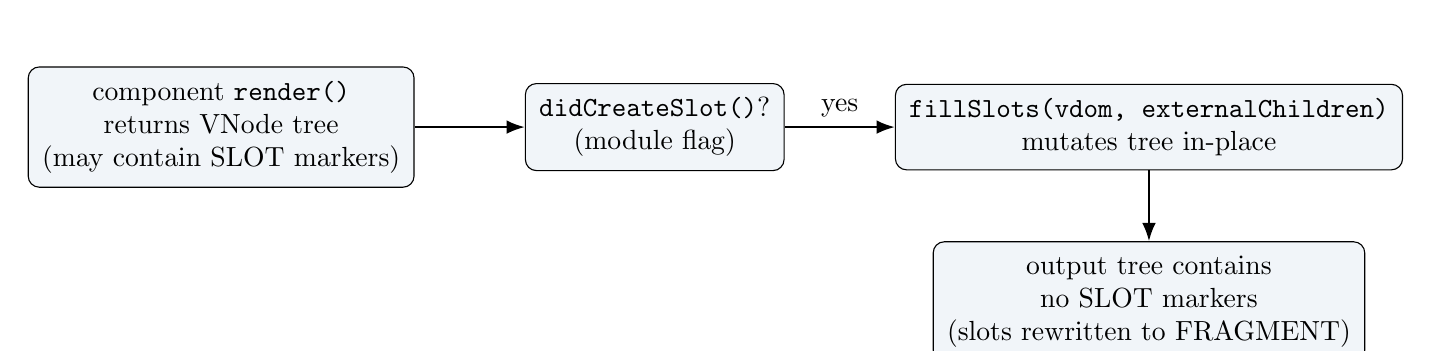
\begin{tikzpicture}[
  node distance=9mm,
  box/.style={draw,rounded corners,fill=RelaxLight,inner sep=5pt,align=center},
  arrow/.style={-Latex,thick}
]
  \node[box] (render) {component \texttt{render()}\\returns VNode tree\\(may contain SLOT markers)};
  \node[box, right=14mm of render] (flag) {\texttt{didCreateSlot()}?\\(module flag)};
  \node[box, right=14mm of flag] (fill) {\texttt{fillSlots(vdom, externalChildren)}\\mutates tree in-place};
  \node[box, below=of fill] (out) {output tree contains\\no SLOT markers\\(slots rewritten to FRAGMENT)};

  \draw[arrow] (render) -- (flag);
  \draw[arrow] (flag) -- node[above]{yes} (fill);
  \draw[arrow] (fill) -- (out);
\end{tikzpicture}
\end{center}

After this rewrite, slots disappear as a concept: mount/patch just see fragments and children arrays.

Slots in the VDOM layer are intentionally small and test-driven:

\begin{itemize}
  \item VNode marker: \texttt{DOM\_TYPES.SLOT} built by \texttt{hSlot()} in \texttt{src/h.ts}
  \item Slot filling algorithm: \texttt{fillSlots(vdom, children)} in \texttt{src/slots.ts}
  \item Specs: \texttt{src/\_\_tests\_\_/slots.test.ts} and \texttt{src/\_\_tests\_\_/component-slots.test.ts}
\end{itemize}

\section{Slot VNodes: \texttt{hSlot} and the SLOT marker}

A slot is represented as a VNode whose \texttt{type} is \texttt{DOM\_TYPES.SLOT}.

In \texttt{src/h.ts}:

\begin{itemize}
  \item \texttt{DOM\_TYPES} includes \texttt{SLOT: 'slot'}.
  \item \texttt{hSlot(children = [])} returns \texttt{\{ type: SLOT, children \}}.
  \item \texttt{hSlot} also sets a module-level flag \texttt{hSlotCalled = true}.
\end{itemize}

That flag is read via \texttt{didCreateSlot()} and reset via \texttt{resetDidCreateSlot()}.

\subsection{Why track \texttt{didCreateSlot}?}

Relax uses this flag as a cheap "did the render tree contain any slots?" signal.
The component renderer (\texttt{src/component.ts}) uses it:

\begin{itemize}
  \item if a slot was created during \texttt{render()}, it calls \texttt{fillSlots(vdom, externalChildren)}
  \item then it resets the flag
\end{itemize}

This avoids doing a full traversal to \emph{search} for slots when there are none.

\paragraph{How the optimization is wired (\texttt{src/component.ts})}

The component render pipeline is:

\begin{enumerate}
  \item call user \texttt{render()} to produce a VNode tree
  \item if any \texttt{hSlot()} call happened while rendering (module flag), run \texttt{fillSlots(vdom, externalChildren)}
  \item reset the module flag so the next render starts clean
\end{enumerate}

This is literally the code:

\begin{verbatim}
if (didCreateSlot()) {
  fillSlots(vdom, this.#children)
  resetDidCreateSlot()
}
\end{verbatim}

\subsection{Authoring model: what the user writes vs. what the runtime sees}

It helps to keep two mental views:

\begin{itemize}
  \item \textbf{Author view}: you "render a slot" and "pass children".
  \item \textbf{Runtime view}: you render a placeholder VNode of type \texttt{SLOT}, then run a rewrite that replaces it.
\end{itemize}

Here's a simple author-level example:

\begin{lstlisting}[language=JavaScript]
// A component with a slot position
const Card = defineComponent({
  render() {
    return h('section', { class: 'card' }, [
      h('header', {}, [h('h2', {}, ['Title'])]),
      h('main', {}, [hSlot([h('em', {}, ['Default body'])])]),
    ])
  },
})

// Call site provides external children
const app = h(Card, {}, [h('p', {}, ['Hello from the outside'])])
mountDOM(app, document.body)

// After slot rewrite, patch/mount only sees normal children under <main>
// (slot marker is gone)
\end{lstlisting}

Even if you never think about slots again, this explains why they're cheap: the renderer doesn't need special mount logic.

So slot filling is a \emph{conditional rewrite pass} executed only when a slot marker was created.

The tests explicitly check this optimization:

\begin{itemize}
  \item \texttt{when the component has slots, the "fillSlot()" function is called}
  \item \texttt{when the component has no slots, the "fillSlot()" function is not called}
\end{itemize}

(See \texttt{src/\_\_tests\_\_/component-slots.test.ts}).

\section{fillSlots(): projecting external children into a component}

The slot filling algorithm lives in \texttt{src/slots.ts}:

\begin{verbatim}
fillSlots(vdom, children)
\end{verbatim}

At a high level:

\begin{itemize}
  \item It traverses a VDOM tree.
  \item It finds SLOT nodes.
  \item It replaces a SLOT node with a FRAGMENT node containing either:
    \begin{itemize}
      \item external content (children passed into the component), or
      \item default slot content (children attached to the SLOT marker).
    \end{itemize}
\end{itemize}

\subsection{Contract}

\begin{itemize}
  \item Input: a rendered VDOM subtree \texttt{vdom}, and an array of \texttt{children} coming from the component call-site.
  \item Output: it mutates the tree in-place.
  \item Post-condition: every SLOT marker encountered is rewritten into a FRAGMENT node.
\end{itemize}

\subsection{A more precise contract: invariants you can rely on}

If you're debugging a slots issue, hand-wavy descriptions aren't enough. The tests assume these invariants:

\begin{itemize}
  \item \textbf{No slot markers survive}: after the rewrite, \texttt{DOM\_TYPES.SLOT} must not appear in the tree that gets mounted/patched.
  \item \textbf{One component = one filling context}: a component only fills slots within the VDOM tree returned by its own \texttt{render()}.
  \item \textbf{External children are late-bound per render}: on every component render, the caller-provided children array is considered "the current external content".
  \item \textbf{Mount/patch remain slot-agnostic}: any observable behavior must reduce to normal fragment/child reconciliation.
\end{itemize}

This design is why slots are "easy" in Relax: they are implemented as a deterministic pre-processing pass.

\subsection*{Diagram: the traversal + rewrite policy}

\begin{center}
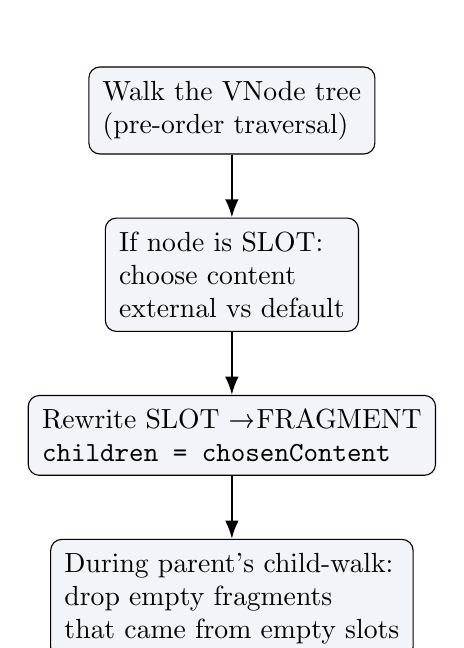
\begin{tikzpicture}[
  node distance=8mm,
  box/.style={draw,rounded corners,fill=RelaxLight,inner sep=5pt,align=left},
  arrow/.style={-Latex,thick}
]
  \node[box] (walk) {Walk the VNode tree\\(pre-order traversal)};
  \node[box, below=of walk] (slot) {If node is SLOT:\\choose content\\external vs default};
  \node[box, below=of slot] (rewrite) {Rewrite SLOT \textrightarrow FRAGMENT\\\texttt{children = chosenContent}};
  \node[box, below=of rewrite] (drop) {During parent's child-walk:\\drop empty fragments\\that came from empty slots};

  \draw[arrow] (walk) -- (slot);
  \draw[arrow] (slot) -- (rewrite);
  \draw[arrow] (rewrite) -- (drop);
\end{tikzpicture}
\end{center}

\paragraph{Why FRAGMENT?}

The renderer needs to splice \emph{zero, one, or many} children into a single position in the parent.
In Relax’s VDOM model, fragments are the standard encoding for ``a list of children with no wrapping element''.
By rewriting slots to fragments, everything downstream (mounting, patching, diffing) can treat the result as normal VDOM.

\subsection{Choosing between default and external content}

When \texttt{fillSlots} sees \texttt{vdom.type === SLOT}, it computes:

\begin{itemize}
  \item \texttt{defaultContent} from \texttt{vdom.children}
  \item \texttt{externalContent} from the passed \texttt{children}
\end{itemize}

Then it uses a simple rule:

\begin{quote}
If external content is provided, it wins. Otherwise the default content is used.
\end{quote}

In code, this is:

\begin{verbatim}
const content = externalContent.length > 0 ? externalContent : defaultContent
\end{verbatim}

This is exactly what \texttt{src/\_\_tests\_\_/slots.test.ts} asserts:

\begin{itemize}
  \item \texttt{set default content if no external content}
  \item \texttt{set the external content if provided}
\end{itemize}

\subsection{Slots with no content are removed}

If a slot has neither default nor external content, Relax removes it.

Implementation detail:

\begin{itemize}
  \item A SLOT node is converted into a FRAGMENT.
  \item If the chosen content is empty, \texttt{vdom.children = []}.
  \item During the parent traversal pass, empty fragments that were slots are dropped.
\end{itemize}

Test: \texttt{remove the slot if no content or default content}.

\paragraph{A subtle implementation detail}

	exttt{fillSlots()} itself doesn't have access to a parent pointer.
So it can’t ``remove the slot node'' directly.
Instead it uses a two-step approach:

\begin{enumerate}
  \item rewrite SLOT \textrightarrow empty FRAGMENT (\texttt{children = []})
  \item during the parent’s child-walk pass, drop empty fragments that were produced by empty slots
\end{enumerate}

That design keeps the algorithm simple and makes behavior local to the traversal.

\subsection{A subtle but crucial point: \texttt{children} is not "DOM children"}

In Relax, component call-sites pass \emph{VNode children}, not DOM nodes.
That means "slot content" participates in the same rules we've already learned:

\begin{itemize}
  \item strings/numbers passed as children are normalized into TEXT VNodes (by \texttt{h()} / child mapping)
  \item arrays are structurally meaningful (fragments flatten in some places; slot-default content has a special shape rule)
  \item children are diffed like any other VNode list after slot filling
\end{itemize}

If you come from Web Components: HTML \texttt{<slot>} projects "real DOM".
Relax is closer to "project a subtree description".
Conceptual reference: \href{https://developer.mozilla.org/en-US/docs/Web/API/Web_components/Using_templates_and_slots}{MDN \texttt{<slot>}}.

\subsection{A code-walk of \texttt{fillSlots} (in plain JavaScript)}

The real implementation is in \texttt{src/slots.ts}, but this version captures the exact intent and shape.
The key is: \textbf{slot rewrite is mutation}, not allocation of a second tree.

\begin{lstlisting}[language=JavaScript]
function fillSlots(vdom, externalChildren) {
  if (!vdom) return

  // 1) Slot node found: rewrite it into a fragment
  if (vdom.type === DOM_TYPES.SLOT) {
    const defaultContent = Array.isArray(vdom.children) ? vdom.children : []
    const passed = Array.isArray(externalChildren) ? externalChildren : []
    const content = passed.length > 0 ? passed : defaultContent

    vdom.type = DOM_TYPES.FRAGMENT

    // Empty slot => become empty fragment; parent traversal later drops it
    if (content.length === 0) {
      vdom.children = []
      return
    }

    // Shape rule: hSlot([defaultContent]) means `content` is [[...]]
    const first = content[0]
    if (Array.isArray(first) && content.length === 1) {
      vdom.children = content
    } else {
      vdom.children = [content]
    }

    return
  }

  // 2) Traverse children, but treat components as opaque boundaries
  if (Array.isArray(vdom.children) && vdom.type !== DOM_TYPES.COMPONENT) {
    const next = []
    for (const child of vdom.children) {
      fillSlots(child, externalChildren)

      // Optional cleanup: drop empty fragments produced by empty slots
      if (child && child.type === DOM_TYPES.FRAGMENT && (!child.children || child.children.length === 0)) {
        continue
      }
      next.push(child)
    }
    vdom.children = next
  }
}
\end{lstlisting}

If you've implemented compilers, this should feel familiar: it's a single-pass rewrite with a few invariants.

\paragraph{Important: the real implementation differs slightly from the teaching version}

In the actual \texttt{src/slots.ts}, external content is set as:

\begin{quote}
fragment children = \texttt{content}
\end{quote}

not \texttt{[content]}. This matters for patching.
If you accidentally wrap external content in another array, you'd introduce an extra nesting level, which would make the fragment children shape wrong.

Interpretation:
	extbf{default content has a special container shape; external content is already a list.}

\subsection{Shape detail: why \texttt{hSlot([defaultContent])} is special}

There’s a slightly odd but intentional shape rule documented in \texttt{src/slots.ts}:

\begin{quote}
\texttt{hSlot([defaultContent])} passes an array whose first element is itself an array.
\end{quote}

So default slot content is often authored like:

\begin{verbatim}
hSlot([ h('span', {}, ['Hello']) ])
\end{verbatim}

In this case the algorithm sees: ``content is an array with a single element, and that element is also an array''.
It preserves that container shape so that:\\
	extbf{a slot expands to exactly one fragment child in the parent}, matching how the tests assert the resulting tree:

\begin{verbatim}
expect(vdom.children).toEqual([hFragment(defaultContent)])
\end{verbatim}

\section{Why fillSlots skips component children during traversal}

The traversal logic in \texttt{fillSlots} explicitly ignores children whose type is \texttt{COMPONENT}.

This is important. Consider:

\begin{itemize}
  \item You are filling a slot for component \texttt{A}.
  \item Inside \texttt{A}'s subtree there might be a nested component \texttt{B} that also uses slots.
\end{itemize}

Relax wants \textbf{each component to fill its own slots} using its own external content.
If the parent traversal reached into component children, it could fill the wrong slots with the wrong content.

Another way to say this: \texttt{fillSlots} treats \texttt{COMPONENT} vnodes as \emph{opaque}. That matches the rest of the renderer: components are patched/mounted as black boxes, and only the component instance is responsible for producing/maintaining its internal subtree.

This is a major boundary rule:

\begin{quote}
Slot rewriting is done per-component and must not cross component vnode boundaries.
\end{quote}

\subsection{Why this boundary matters in real apps}

If the parent traversal rewrote nested component internals, you'd get extremely confusing coupling:

\begin{itemize}
  \item A parent could accidentally fill a child component's slot with the wrong content.
  \item A refactor that wraps content in an extra component would silently change slot behavior.
  \item Slot filling would become order-dependent across renders (hard to test, hard to reason about).
\end{itemize}

By treating components as tuples of \texttt{(props, children)} and letting each component own its own slot rewrite,
Relax preserves a clean mental model: \textbf{slots are part of the component API surface, not the global tree.}

It also aligns with how the renderer treats components elsewhere:
components are patched/mounted as black boxes whose internal VDOM is managed by the component instance.

\subsection{From-scratch example: why crossing the boundary would be a bug}

Imagine this:

\begin{lstlisting}[language=JavaScript]
const Inner = defineComponent({
  render() {
    return h('div', {}, [hSlot([h('em', {}, ['Inner default'])])])
  },
})

const Outer = defineComponent({
  render() {
    return h('section', {}, [
      // Outer has a slot too
      hSlot([h('span', {}, ['Outer default'])]),

      // And it renders Inner
      h(Inner, {}, []),
    ])
  },
})

// Call site passes ONE set of children to Outer
mountDOM(h(Outer, {}, [h('b', {}, ['Projected into Outer'])]), document.body)
\end{lstlisting}

If \texttt{fillSlots} descended into the \texttt{Inner} component vnode,
it could (incorrectly) fill Inner's slot with Outer's external children.
That would mean Inner's content depends on who rendered it (bad encapsulation).

Relax avoids this by making \texttt{COMPONENT} a hard boundary during traversal.

This behavior is tested in \texttt{src/\_\_tests\_\_/slots.test.ts}:

\begin{itemize}
  \item \texttt{ignores slots whose parent is a component (they are handled by the component)}
\end{itemize}

\section{Slots in real components (\texttt{component-slots.test.ts})}

The integration tests show what authoring looks like.

\subsection{Basic projection}

\texttt{can have a slot where external content can be inserted}:

\begin{itemize}
  \item Component renders \texttt{<div>\{slot\}</div>}.
  \item Call site provides \texttt{<span>Hello</span>}.
  \item The mounted DOM contains the span.
\end{itemize}

\subsection{Default content}

\texttt{when no external content is provided, the default content is used}.

This is the standard "slot fallback" semantics.

\subsection{Conditional slots}

\texttt{conditionally rendered slots} verifies that slots can appear/disappear depending on component state, and the patcher will reconcile accordingly.

This is where slots meet the patching story from Chapter 8: slot output is just fragments and normal children after filling.

\subsection{Updating slot content between renders}

\texttt{slot content updated between renders} has a container component that alternates between:

\begin{itemize}
  \item a single \texttt{<span>Hello</span>}
  \item or two children \texttt{<p>World</p><span>!</span>}
\end{itemize}

The important point: slot external content is treated like regular children arrays and diffed normally after filling.

Practically:

\begin{itemize}
  \item the container component re-renders and passes a different external children array
  \item the slotted component re-renders, sees a slot marker, and re-runs \texttt{fillSlots}
  \item after that rewrite, the patcher sees ordinary FRAGMENT/ELEMENT/TEXT children and reconciles them
\end{itemize}

\subsection{Nested slots inside lists}

The last integration scenario in \texttt{component-slots.test.ts} is important because it looks like ``normal app code'':
build a list, render repeated components, and project a different child into each one.

Mentally, it's just two loops:

\begin{itemize}
  \item The parent maps \texttt{items} to \texttt{TableRow} component vnodes.
  \item Each \texttt{TableRow} render tree contains a slot marker in a \texttt{<td>}.
\end{itemize}

In author-level code (simplified):

\begin{lstlisting}[language=JavaScript]
const TableRow = defineComponent({
  render() {
    return h('tr', {}, [
      h('td', {}, [hSlot([h('em', {}, ['(empty)'])])]),
    ])
  },
})

const Table = defineComponent({
  render() {
    const titles = ['One', 'Two']
    return h('table', {}, [
      h('tbody', {}, titles.map((t) =>
        // Each row receives different external children.
        h(TableRow, {}, [t])
      )),
    ])
  },
})
\end{lstlisting}

The slot rewrite story stays exactly the same:
each \texttt{TableRow} instance stores its own external children (here: \texttt{['One']} or \texttt{['Two']}) and fills the slot while rendering.

Senior rule of thumb:
\begin{quote}
If you can explain repeated slots-in-lists, you understand slots. Everything else is a smaller case.
\end{quote}

\section{Walking the integration tests in slow motion (event-loop + render pipeline)}

Slots can feel magical until you align them with the component pipeline from earlier chapters.
At a high level, mounting a component with slot children looks like this:

\begin{enumerate}
  \item \textbf{Mount begins} at the parent vnode.
  \item When the renderer hits a \texttt{COMPONENT} vnode:
    \begin{enumerate}
  \item create the component instance
  \item store external children array on the instance (conceptually: \texttt{this.\#children})
  \item call \texttt{render()} to get an internal subtree
  \item if \texttt{didCreateSlot()} was set by \texttt{hSlot()}, run \texttt{fillSlots(subtree, this.\#children)}
  \item mount the rewritten subtree to DOM
    \end{enumerate}
\end{enumerate}

In other words, slot filling is part of "turn render output into mountable VDOM".
The patcher never sees a slot marker.

This is why the spy tests in \texttt{component-slots.test.ts} are important: they confirm the optimization boundary is hooked up correctly.

\texttt{slot in a nested component} uses a table row component with a slot in a \texttt{<td>}.
The parent maps titles \texttt{['One','Two']} into multiple \texttt{TableRow} instances.

This shows that slot content can be:

\begin{itemize}
  \item a raw string child (which becomes a TEXT VNode via \texttt{h()} normalization)
  \item repeated many times across a list of nested components
\end{itemize}

\section{Takeaways}

\begin{itemize}
  \item Slots are recorded as a VNode marker produced by \texttt{hSlot()}.
  \item Slot filling is a tree rewrite: SLOT \(\rightarrow\) FRAGMENT with chosen content.
  \item External content wins over default content.
  \item Empty slots are removed by dropping empty fragments.
  \item Each component fills its own slots; parent traversal does not cross component boundaries.
\end{itemize}

\section{Walking the tests: what they prove}

Slots are specified in two layers: a pure tree-rewrite unit suite and a DOM-level integration suite.

\subsection{Unit semantics (\texttt{src/\_\_tests\_\_/slots.test.ts})}

\begin{description}
  \item[remove the slot if no content or default content] Proves the empty-slot removal behavior: a slot with no default and no external content is eliminated (via empty-fragment dropping).
  \item[set default content if no external content] Proves fallback behavior and the default-content shape rule. The assertion expects \texttt{[hFragment(defaultContent)]}.
  \item[set the external content if provided] Proves the precedence rule: external content overrides default content.
  \item[ignores slots whose parent is a component] Proves the traversal boundary rule: \texttt{fillSlots} must not rewrite nested component internals.
\end{description}

\subsection{Integration semantics (\texttt{src/\_\_tests\_\_/component-slots.test.ts})}

\begin{description}
  \item[can have a slot where external content can be inserted] Proves end-to-end projection into mounted DOM.
  \item[default content is used] Proves fallback behavior at DOM level.
  \item[slot is empty] Proves empty slots become empty output (no wrapper nodes appear).
  \item[conditionally rendered slots] Proves slots can appear/disappear and patch correctly when state changes.
  \item[slot content updated between renders] Proves that changing the external children array results in normal DOM reconciliation after slot rewrite.
  \item[slot in a nested component] Proves nested component usage with lists and primitive children (strings become text nodes via \texttt{h()} normalization).
  \item[fillSlots spy tests] Proves the \texttt{didCreateSlot()} optimization works: slot rewrite only runs when \texttt{hSlot()} was actually used.
\end{description}

\section{Online resources}

\begin{itemize}
  \item Web Components: \href{https://developer.mozilla.org/en-US/docs/Web/API/Web_components/Using_templates_and_slots}{MDN \texttt{<slot>} (conceptual comparison)}
  \item Vue: \href{https://vuejs.org/guide/components/slots.html}{Slots and content projection}
  \item React: \href{https://react.dev/learn/passing-props-to-a-component#passing-jsx-as-children}{Passing JSX as children}
  \item SolidJS (conceptual): \href{https://www.solidjs.com/docs/latest#children}{Children utilities}
\end{itemize}

\section{Common pitfalls (senior notes)}

\begin{itemize}
  \item \textbf{Mistaking slots for "render props"}: Relax slots are structural children, not callbacks. If you need code execution with parameters, pass functions as props.
  \item \textbf{Forgetting the rewrite step exists}: by the time \texttt{mountDOM/patchDOM} runs, there is no slot node. Debug by inspecting the post-rewrite VDOM.
  \item \textbf{Component-boundary confusion}: if your slot isn't filling, check where you placed \texttt{hSlot()} -- it must be inside the component that receives the children.
  \item \textbf{Default content shape surprises}: remember that \texttt{hSlot([defaultContent])} uses a container shape that becomes a single fragment child.
\end{itemize}

If you internalize one idea: \textbf{Relax slots are a simple, deterministic rewrite into fragments}. Everything else follows.

\section{Performance notes (why this is fast in practice)}

Two design choices keep this lightweight:

\begin{itemize}
  \item \textbf{Conditional traversal}: the \texttt{didCreateSlot()} flag lets the component skip traversal when there are no slots.
  \item \textbf{In-place rewrite}: \texttt{fillSlots} mutates existing vnode objects. No cloning of the full tree.
\end{itemize}

That matters because slot filling runs on every render where slots are present.
This is the same kind of micro-optimization you see in production UI frameworks: avoid whole-tree work unless a feature is actually used.

Reference (conceptual): \href{https://react.dev/learn/render-and-commit}{React render/commit mental model}.

\section{Exercises}

\begin{enumerate}
  \item Modify the \texttt{fillSlots} teaching implementation so it matches \texttt{src/slots.ts} exactly---especially the external-content shape.
  \item Write a small component pair \texttt{Outer/Inner} (like the boundary example) and predict what would go wrong if traversal crossed into components.
  \item Explain (in 3-5 sentences) why "slots compiled away into fragments" simplifies the patcher.
\end{enumerate}

\section{Chapter summary}

\begin{itemize}
  \item Relax implements slots as a VNode marker (\texttt{DOM\_TYPES.SLOT}) created by \texttt{hSlot()}.
  \item Slot behavior is a deterministic rewrite pass: SLOT is rewritten to FRAGMENT containing either external or default content.
  \item Component vnodes are traversal boundaries: each component owns slot filling for its own render output.
  \item After filling, mount and patch operate on normal VDOM only---no special slot logic downstream.
\end{itemize}

\chapter{HRBR Signals: a Small Deterministic Reactive Graph}

Part III begins the HRBR runtime. Unlike the VDOM runtime (\texttt{src/*}), HRBR is a "compiled fast path" whose job is to:

\begin{itemize}
  \item track fine-grained dependencies (signals)
  \item schedule updates deterministically (scheduler lanes)
  \item update DOM directly in blocks (later chapters)
\end{itemize}

This chapter focuses on the reactive graph implementation in \texttt{runtime/signals.ts}.

\section{Why signals exist (and why HRBR needs them)}

Up to this point, Relax updates UI via a Virtual DOM pipeline: you re-run \texttt{render()}, diff children, then patch the DOM.
That model is flexible and easy to reason about, but it can do more work than necessary when updates are tiny and frequent.

Signals exist to make a different trade-off:

\begin{quote}
Track \emph{exactly} which computations depend on a value, and when that value changes, re-run only those computations.
\end{quote}

This is the core HRBR idea: the compiler can translate template expressions into tiny computations (effects/memos) that update very specific DOM nodes.
So instead of reconciling a large subtree, a signal write can result in “update this text node”.

Compare the philosophies:

\begin{itemize}
  \item \textbf{VDOM:} change state \textrightarrow rerender \textrightarrow reconcile structure.
  \item \textbf{Signals:} change signal \textrightarrow schedule dependent computations \textrightarrow update exactly where read.
\end{itemize}

For external context (not Relax-specific), see:
\href{https://www.solidjs.com/docs/latest#signals}{SolidJS signals} (fine-grained model) and
\href{https://react.dev/learn/render-and-commit}{React render/commit} (VDOM model).

\section{Public API: the contract we have to satisfy}

The file \texttt{runtime/index.ts} exports these symbols from \texttt{runtime/signals.ts}:

\begin{itemize}
  \item \texttt{createSignal(initial) -> [read, write]}
  \item \texttt{createEffect(fn, options?) -> \{ dispose() \}}
  \item \texttt{createMemo(fn, opts?) -> readMemo}
  \item \texttt{batch(fn) -> result}
  \item \texttt{untrack(fn) -> result}
\end{itemize}

The executable specification lives in:

\begin{itemize}
  \item \texttt{runtime/\_\_tests\_\_/signals.test.ts}
  \item \texttt{runtime/\_\_tests\_\_/signals.determinism.test.ts}
  \item \texttt{runtime/\_\_tests\_\_/signals.fuzz.test.ts}
\end{itemize}

\section{Mental model}

You can read \texttt{runtime/signals.ts} as a deliberately small version of a Solid-like graph:

\begin{itemize}
  \item A \textbf{signal} is a node with a current value and a list of observers.
  \item An \textbf{effect} is a computation that re-runs when its dependencies (signals/memos) change.
  \item A \textbf{memo} is a computation that behaves like a derived signal.
\end{itemize}

Two design constraints keep showing up in the implementation and tests:

\begin{enumerate}
  \item \textbf{Determinism}: observer notification runs in stable creation order.
  \item \textbf{Leak-safety}: disposing a computation must detach it from all sources.
\end{enumerate}

There’s a third, more pragmatic constraint you’ll see in the code:

\begin{itemize}
  \item \textbf{Low ceremony}: everything is implemented with plain objects and a few intrusive linked lists.
\end{itemize}

This is not a ``fully-featured'' reactive system; it’s a compact kernel meant to be embedded into compiled blocks.

\section{The tiny contract (keep this in your head)}

Signals are small, so their contract can be crisp:

\begin{itemize}
  \item \textbf{Read} returns a value and optionally registers a dependency edge.
  \item \textbf{Write} updates the value and schedules observers \emph{in deterministic order}.
  \item \textbf{Effect} runs once initially, then re-runs when its dependencies change.
  \item \textbf{Memo} caches a derived value and notifies dependents when it changes.
  \item \textbf{batch(fn)} coalesces multiple writes into a single downstream flush.
  \item \textbf{untrack(fn)} temporarily disables dependency capture.
\end{itemize}

And the failure modes we must avoid (the tests are built around these):

\begin{itemize}
  \item \textbf{Nondeterminism}: the observer order changes across runs.
  \item \textbf{Leaks}: disposed computations still run after future writes.
  \item \textbf{Re-entrancy recursion}: an effect writes to what it reads and causes stack overflow.
  \item \textbf{Stale dependencies}: conditional reads don’t update subscriptions.
\end{itemize}

\section{Diagram: signals graph (sources \textrightarrow computations \textrightarrow derived values)}
The runtime is easiest to visualize as a graph where reads register edges and writes schedule computations:

\begin{center}
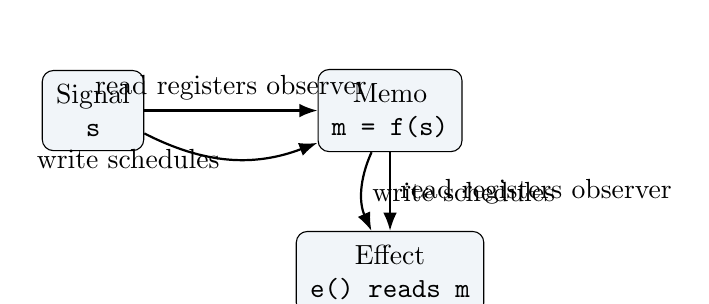
\begin{tikzpicture}[
  node distance=10mm,
  box/.style={draw,rounded corners,fill=RelaxLight,inner sep=5pt,align=center},
  arrow/.style={-Latex,thick}
]
  \node[box] (s) {Signal\\\texttt{s}};
  \node[box, right=22mm of s] (m) {Memo\\\texttt{m = f(s)}};
  \node[box, below=of m] (e) {Effect\\\texttt{e() reads m}};

  \draw[arrow] (s) -- node[above]{read registers observer} (m);
  \draw[arrow] (m) -- node[right]{read registers observer} (e);
  \draw[arrow] (s) to[bend right=24] node[left]{write schedules} (m);
  \draw[arrow] (m) to[bend right=24] node[right]{write schedules} (e);
\end{tikzpicture}
\end{center}

The rest of this chapter explains how Relax keeps this graph deterministic and leak-safe with intrusive linked lists.

\section{Core data structures: intrusive lists for stable order}

In \texttt{runtime/signals.ts} you will see a set of internal types:

\begin{itemize}
  \item \texttt{SignalNode<T>} holds \texttt{value} and an intrusive doubly-linked list of observers: \texttt{observersHead/observersTail}.
  \item \texttt{Computation} represents an effect or memo computation.
  \item \texttt{ObserverLink} is the node stored in the signal's observer list.
  \item \texttt{SourceLink} is a reverse edge stored on the computation so it can detach from sources on re-run/dispose.
\end{itemize}

The key technique: when a computation reads a signal, \texttt{addObserver(node, currentComputation)} inserts the computation into the signal's observer list \emph{sorted by computation id}.

Computation ids come from a global counter:

\begin{verbatim}
let nextId = 0

comp._id = nextId++
\end{verbatim}

Because ids are monotonically increasing, the observer list is stable and deterministic by construction.

\subsection{Why two linked lists (observer list + source list)?}

Each dependency edge is represented twice:

\begin{itemize}
  \item a forward link in the signal’s \texttt{observersHead/observersTail} list (who should be scheduled when the signal changes)
  \item a reverse link in the computation’s \texttt{sourcesHead/sourcesTail} list (what should be detached before re-run/dispose)
\end{itemize}

This dual representation is what makes ``conditional dependencies'' safe: each run starts by detaching previous sources and then re-registering based on the reads that actually occur.

\subsection{Diagram: forward observers vs. reverse sources}

This is the part that makes signals feel like a real runtime (not a toy): every edge is represented twice.

\begin{itemize}
  \item The \textbf{forward edge} lives on the signal: ``who should I notify when I change?''
  \item The \textbf{reverse edge} lives on the computation: ``what did I subscribe to last run, so I can detach?''
\end{itemize}

\begin{center}
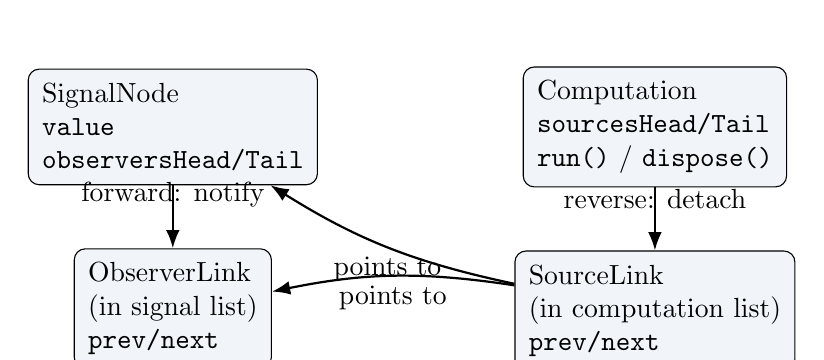
\begin{tikzpicture}[
  node distance=8mm,
  box/.style={draw,rounded corners,fill=RelaxLight,inner sep=5pt,align=left},
  arrow/.style={-Latex,thick}
]
  \node[box] (sig) {SignalNode\\\texttt{value}\\\texttt{observersHead/Tail}};
  \node[box, right=26mm of sig] (comp) {Computation\\\texttt{sourcesHead/Tail}\\\texttt{run()} / \texttt{dispose()}};

  \node[box, below=of sig] (ol) {ObserverLink\\(in signal list)\\\texttt{prev/next}};
  \node[box, below=of comp] (sl) {SourceLink\\(in computation list)\\\texttt{prev/next}};

  \draw[arrow] (sig) -- node[above]{forward: notify} (ol);
  \draw[arrow] (comp) -- node[above]{reverse: detach} (sl);
  \draw[arrow] (sl) to[bend left=10] node[below]{points to} (sig);
  \draw[arrow] (sl) to[bend right=10] node[below]{points to} (ol);
\end{tikzpicture}
\end{center}

In \texttt{runtime/signals.ts}, this is the practical outcome:

\begin{itemize}
  \item \texttt{addObserver(node, comp)} inserts an \texttt{ObserverLink} into \texttt{node.observers...}
  \item and it appends a \texttt{SourceLink} into \texttt{comp.sources...} that points back to that observer link
  \item \texttt{unlinkAllSources(comp)} walks \texttt{comp.sources...} and removes each referenced observer link from its signal
\end{itemize}

Senior takeaway:
\begin{quote}
If you don't keep the reverse list, you can't implement conditional dependencies without leaks.
\end{quote}

\section{Dependency capture: \texttt{currentComputation}}

Reactive systems need a way to know "who is currently running".

This file uses a single global pointer:

\begin{verbatim}
let currentComputation: Computation | null
\end{verbatim}

\subsection{Signal reads}

In \texttt{createSignal()}, the reader is:

\begin{itemize}
  \item return \texttt{node.value}
  \item if \texttt{currentComputation != null}, also call \texttt{addObserver(node, currentComputation)}
\end{itemize}

That means dependencies are collected by running the effect/memo function and letting reads "register".

\subsubsection{Mechanics: the global pointer trick}

The \texttt{currentComputation} pointer is the entire core of dependency tracking.
When a computation is running, it sets this global.
Signal reads check it and attach the dependency edge.

Here’s a very small teaching implementation in plain JavaScript (not the real Relax code):

\begin{lstlisting}[language=JavaScript]
let currentComputation = null

function createSignal(initial) {
  const node = { value: initial, observers: [] }

  function read() {
    if (currentComputation) node.observers.push(currentComputation)
    return node.value
  }

  function write(next) {
    const nextValue = typeof next === 'function' ? next(node.value) : next
    if (Object.is(nextValue, node.value)) return
    node.value = nextValue

    for (const comp of node.observers) {
      comp.run()
    }
  }

  return [read, write]
}

function createEffect(fn) {
  const comp = {
    run() {
      const prev = currentComputation
      currentComputation = comp
      try {
        fn()
      } finally {
        currentComputation = prev
      }
    },
  }
  comp.run()
  return { dispose() {} }
}
\end{lstlisting}

Relax’s real implementation adds the hard parts:

\begin{itemize}
  \item leak-safety via a reverse list (so it can detach old edges)
  \item deterministic order via monotonically increasing ids + sorted insertion
  \item correct batching + re-entrancy via a pending set and deterministic flush
\end{itemize}

\paragraph{No dedupe (by design)}

You may notice \texttt{addObserver()} explicitly does not deduplicate observers.
This is safe because every run begins with \texttt{unlinkAllSources(comp)}, which removes all prior edges.
So duplicates can only occur within a single run, and a well-behaved effect/memo typically reads each signal at most once.

\subsection{\texttt{untrack(fn)}}

\texttt{untrack(fn)} temporarily sets \texttt{currentComputation = null} while executing \texttt{fn}.

Spec (\texttt{runtime/\_\_tests\_\_/signals.test.ts}):

\begin{itemize}
  \item \texttt{untrack prevents dependency registration}
\end{itemize}

In other words: you can read a signal without subscribing.

\section{Writes: schedule observers, preserve order}

In \texttt{createSignal()}, the writer:

\begin{enumerate}
  \item computes \texttt{nextValue} (supports "functional set" style)
  \item bails out if \texttt{Object.is(nextValue, node.value)}
  \item updates \texttt{node.value}
  \item walks the observer list and schedules each observer
\end{enumerate}

There’s a subtle but important line in the loop:

\begin{quote}
Capture \texttt{next} first, because running an observer can unsubscribe/resubscribe and mutate the list.
\end{quote}

In code (comments preserved):

\begin{verbatim}
const next = cur.next
scheduleComputation(cur.comp)
cur = next
\end{verbatim}

This ensures we traverse the original linked list in deterministic order.

\subsection*{Diagram: observer notification preserves creation order}
Observer lists are kept in stable creation order (by computation id). A write walks that list and schedules computations without losing determinism:

\begin{center}
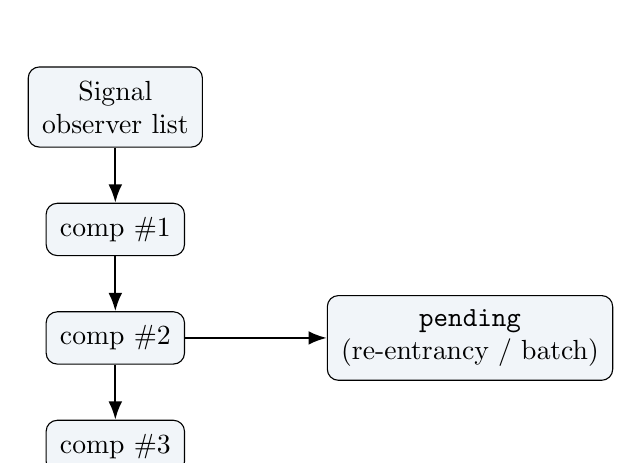
\begin{tikzpicture}[
  node distance=7mm,
  box/.style={draw,rounded corners,fill=RelaxLight,inner sep=5pt,align=center},
  arrow/.style={-Latex,thick}
]
  \node[box] (sig) {Signal\\observer list};
  \node[box, below=of sig] (c1) {comp \#1};
  \node[box, below=of c1] (c2) {comp \#2};
  \node[box, below=of c2] (c3) {comp \#3};
  \node[box, right=18mm of c2] (pend) {\texttt{pending}\\(re-entrancy / batch)};

  \draw[arrow] (sig) -- (c1);
  \draw[arrow] (c1) -- (c2);
  \draw[arrow] (c2) -- (c3);
  \draw[arrow] (c2) -- (pend);
\end{tikzpicture}
\end{center}

The key implementation trick is the one shown in the code snippet above: capture \texttt{next} before scheduling so list mutation during computation runs doesn't break traversal.

\paragraph{What gets scheduled?}

When a signal is written, Relax schedules the dependent computations.
Scheduling does not necessarily mean ``run immediately'' (see batching and lanes), but it always preserves the \emph{creation order} contract.

\subsection{A precise code-walk: \texttt{scheduleComputation} and the \texttt{pending} set}

All the tricky correctness properties (re-entrancy, batching, lane scheduling) flow through one choke point:
	\texttt{scheduleComputation(computation)}.

In the real implementation (\texttt{runtime/signals.ts}), there are four gates.
Reading them as a ruleset helps:

\begin{enumerate}
  \item \textbf{Disposed computations are inert.}
  \item \textbf{Running computations don't re-enter.} If a computation schedules itself while running, it is queued in \texttt{pending} and flushed after the current stack unwinds.
  \item \textbf{Lane-aware computations don't run inline.} If a computation has \texttt{\_schedule}, scheduling is delegated to the runtime scheduler.
  \item \textbf{Batching defers work.} If \texttt{isBatching > 0}, add to \texttt{pending} instead of running.
\end{enumerate}

Here's the same logic in a teaching version (simplified JavaScript), preserving the ordering of checks:

\begin{lstlisting}[language=JavaScript]
function scheduleComputation(comp) {
  if (comp._disposed) return

  // Re-entrancy: don't recurse.
  if (comp._running) {
    pending.add(comp)
    return
  }

  // Lane scheduling: hand off to the scheduler.
  if (comp._schedule) {
    comp._schedule(comp)
    return
  }

  // Batching: defer until end of outer batch.
  if (isBatching > 0) {
    pending.add(comp)
    return
  }

  // Default: run inline.
  comp.run()
}
\end{lstlisting}

\subsubsection{Why re-entrancy and batching share the same queue}

At first glance, using one \texttt{pending} set for two distinct situations looks odd.
It's actually a good simplification because both situations mean the same thing:

\begin{quote}
We are not allowed to run this computation right now, but we must not lose the fact that it became dirty.
\end{quote}

The only additional requirement is determinism.
That's why \texttt{flushPendingIfNeeded()} sorts the set by \texttt{\_id} before scheduling.

\subsubsection{Timeline: the re-entrancy convergence test}

Spec: \texttt{re-entrancy: effect that schedules itself via writes does not recurse infinitely}.

The effect is:

\begin{lstlisting}[language=JavaScript]
createEffect(() => {
  const v = s()
  seen.push(v)
  if (v < 3) setS(v + 1)
})
\end{lstlisting}

The important thing is not just that it ends at \texttt{3}, but that it does not recurse.
The run looks like this:

\begin{enumerate}
  \item Start run: comp becomes \texttt{\_running = true}
  \item Reads \texttt{s()} (dependency edge registered)
  \item Calls \texttt{setS(v + 1)} which tries to schedule the same computation
  \item Because it is \texttt{\_running}, scheduling goes to \texttt{pending} (no re-entry)
  \item End run: \texttt{\_running = false}, then we flush \texttt{pending}
\end{enumerate}

This repeats until the signal hits 3.
That is exactly why the expected log is deterministic: \texttt{[0, 1, 2, 3]}.

Reference (conceptual background): Solid's reactivity avoids re-entrancy recursion via queuing and batching as well:
\href{https://www.solidjs.com/docs/latest#execution-order}{Solid: execution order}.

\section{Effects: cleanup, re-run, disposal}

\subsection{Cleanup semantics}

Effects may return an optional cleanup function:

\begin{verbatim}
createEffect(() => {
  ...
  return () => cleanup()
})
\end{verbatim}

The runtime guarantees cleanup runs:

\begin{itemize}
  \item before an effect re-runs
  \item when the effect is disposed
\end{itemize}

Spec: \texttt{effect cleanup runs before re-run and on dispose}.

In code, the cleanup is stored on the computation object as \texttt{comp.cleanup} and executed in a try/finally block both in \texttt{run()} and \texttt{dispose()}.

\subsection{Detaching and resubscribing: \texttt{unlinkAllSources(comp)}}

Before each run, the runtime calls \texttt{unlinkAllSources(comp)}.
That function walks the computation's \texttt{sourcesHead} list and unlinks each corresponding \texttt{ObserverLink} from the signal's observer list.

This gives the common reactive invariant:

\begin{quote}
An effect's dependencies are exactly the signals it read during its last run.
\end{quote}

It also enables conditional dependencies (read signal A in one run, read signal B in another) without leaking observers.

\subsection{Conditional dependencies in slow motion (the reason \texttt{unlinkAllSources} exists)}

Conditional dependencies are the most common place reactive systems silently leak.
The problem looks like this:

\begin{quote}
An effect reads \texttt{a()} in one run, but reads \texttt{b()} in the next run. If you never detach old edges, the effect ends up subscribed to both forever.
\end{quote}

Relax avoids this by making \texttt{unlinkAllSources(comp)} step 0 of every run.
Then the effect/memo re-subscribes only to the signals it \emph{actually reads} this time.

Here's a minimal example to build intuition:

\begin{lstlisting}[language=JavaScript]
const [useA, setUseA] = createSignal(true)
const [a, setA] = createSignal(0)
const [b, setB] = createSignal(0)

createEffect(() => {
  if (useA()) {
    console.log('A path:', a())
  } else {
    console.log('B path:', b())
  }
})
\end{lstlisting}

Now imagine this sequence:

\begin{enumerate}
  \item Initial run: \texttt{useA() == true} so the effect reads \texttt{useA()} and \texttt{a()}.
  \item Flip to \texttt{false}: the effect re-runs, but now it reads \texttt{useA()} and \texttt{b()}.
\end{enumerate}

If the runtime does not detach, a later \texttt{setA(...)} would still schedule the effect even though it no longer reads \texttt{a()}.
That is wasted work and (in large graphs) becomes a performance cliff.

\subsubsection{What the implementation guarantees}

This is the practical contract enforced by the forward+reverse lists:

\begin{itemize}
  \item Before each run, unlink all previously tracked sources.
  \item During the run, every signal/memo read adds new source links.
  \item After the run, the computation is subscribed to exactly the set of reads that occurred.
\end{itemize}

That is why the dual list structure matters: the reverse list is what makes detaching cheap and precise.

Conceptual reference: Solid's explanation of fine-grained dependency tracking is very similar:
\href{https://www.solidjs.com/docs/latest#how-it-works}{Solid: how it works}.

\paragraph{Leak-safety note}

	\texttt{unlinkAllSources()} also deliberately nulls out fields on the link objects (with \texttt{@ts-expect-error} comments).
That’s not required for correctness, but it makes accidental retention less likely in this prototype implementation.

\section{Non-negotiable guarantees (what must remain true)}

If you want to understand signals fast, read the tests first.
They encode the contract in a way that prevents “almost works” implementations.

\subsection{Core semantics: \texttt{runtime/\_\_tests\_\_/signals.test.ts}}

The suite asserts:

\begin{itemize}
  \item dependency tracking (reads register; writes re-run)
  \item \texttt{Object.is} bail-out prevents no-op writes from causing work
  \item \texttt{untrack} disables edge registration
  \item \texttt{batch} is a flush boundary (including nested batching)
  \item cleanup is run before re-run and on dispose
  \item dispose fully detaches
  \item re-entrancy converges without recursive re-entry
  \item non-sync lanes schedule through the runtime scheduler (tests intercept \texttt{setTimeout})
  \item memos behave like derived signals and notify dependents
\end{itemize}

\subsubsection{A senior reading of the suite: what it forces in the implementation}

The most important thing these tests enforce is that signals are not just a pub/sub primitive.
They are a mini runtime with strict invariants:

\begin{itemize}
  \item \textbf{Idempotent writes}: \texttt{Object.is} bail-out means no "useless work" on repeated values.
  \item \textbf{Precise tracking}: \texttt{untrack} demonstrates that dependency capture is opt-in per read, not an ambient global subscription.
  \item \textbf{Deterministic event ordering}: effect order must be stable even under batching.
  \item \textbf{Cleanup correctness}: cleanup must run before the next run, not after.
\end{itemize}

If you've ever debugged a real UI bug caused by nondeterministic ordering, you'll appreciate why determinism is treated as a contract, not an "implementation detail".

\subsection{Determinism + leak-ish checks: \texttt{signals.determinism.test.ts}}

The determinism suite checks a stronger property:
\emph{same seed + same operations produce identical logs across two fresh graphs}.

That forces the runtime to be stable in ways a single unit test won’t catch.
It also includes a practical disposal check: once an effect is disposed, later writes must not produce any new log entries for it.

\subsection{Fuzz/property checks: \texttt{signals.fuzz.test.ts}}

The fuzz test generates nested batches, sets, and disposals.
The primary assertion is determinism (two runs produce identical logs).
There is also a “smoke” property related to disposal: if effects were disposed, later mass-writes shouldn’t explode log volume.

\subsection{Dispose}

Disposing an effect sets \texttt{\_disposed} and detaches from all sources.

Specs:

\begin{itemize}
  \item \texttt{disposed effects fully detach: further writes do not schedule work}
  \item leak-ish checks in \texttt{runtime/\_\_tests\_\_/signals.determinism.test.ts}
\end{itemize}

\section{Re-entrancy: scheduling while running}

In \texttt{scheduleComputation(computation)} there is an explicit re-entrancy rule:

\begin{itemize}
  \item if the computation is \texttt{\_running}, do not recursively call \texttt{run()}
  \item instead, add it to a \texttt{pending} \texttt{Set}
\end{itemize}

Then \texttt{flushPendingIfNeeded()} runs pending computations after the current run unwinds.

\subsection{Two reasons computations are delayed}

The same \texttt{pending} set is used for two distinct delay cases:

\begin{itemize}
  \item \textbf{re-entrancy}: a computation schedules itself while it’s already running
  \item \textbf{batching}: writes should not trigger intermediate runs until the batch boundary
\end{itemize}

Both cases end up in the same deterministic flush code path.

Spec: \texttt{re-entrancy: effect that schedules itself via writes does not recurse infinitely}.

The test constructs an effect that reads a signal and writes it again until a fixed point is reached.
The expected (deterministic) log is:

\begin{verbatim}
[0, 1, 2, 3]
\end{verbatim}

\section{Batching: a flush boundary}

\texttt{batch(fn)} increments \texttt{isBatching} and makes writes collect work into \texttt{pending}.
When the outer-most batch finishes, it flushes the pending set sorted by computation id.

Specs (\texttt{runtime/\_\_tests\_\_/signals.test.ts}):

\begin{itemize}
  \item \texttt{batch groups multiple writes into a single effect re-run}
  \item \texttt{batch() is a flush boundary: nested batches still only produce one re-run after outer finishes}
  \item \texttt{batch() returns the callback result and preserves deterministic effect order after flush}
\end{itemize}

This is the first place you see HRBR's theme: \emph{deterministic scheduling is part of the user-facing contract}.

\paragraph{Implementation detail: deterministic flush}

At batch end, pending computations are flushed by sorting on \texttt{\_id}:

\begin{verbatim}
Array.from(pending).sort((a,b) => a._id - b._id)
\end{verbatim}

This is why the tests can assert stable order like \texttt{['a:2', 'b:2']}.

\section{Memos: derived signals with equality}

\texttt{createMemo(fn, opts?)} creates a computation whose output is stored in a \texttt{SignalNode<T>}.

Important details:

\begin{itemize}
  \item the memo lazily computes on first read (\texttt{if (!hasValue) comp.run()})
  \item it supports an equality function \texttt{opts.equals} (defaults to \texttt{Object.is})
  \item it notifies observers only when the memo value actually changes
\end{itemize}

Spec: \texttt{createMemo computes from signals and updates dependents}.

\paragraph{Memo invalidation path}

When the memo value changes, it walks \texttt{node.observersHead} and schedules each observer computation.
So effects that read a memo are notified exactly like effects that read a base signal.

\section{Lanes: effects can be scheduled via the runtime scheduler}

\texttt{createEffect} accepts options:\\
\texttt{\{ lane?: Lane, budgetMs?: number \}}.

If \texttt{lane === 'sync'} (the default), the initial run executes immediately.

If \texttt{lane !== 'sync'}, \texttt{createEffect} creates a scheduler via \texttt{createScheduler()} (from \texttt{runtime/scheduler.ts}) and schedules runs into that lane.

\subsection{How non-sync lanes are tested}

In \texttt{runtime/\_\_tests\_\_/signals.test.ts}, the tests override \texttt{globalThis.setTimeout} to capture scheduled flush callbacks into an array.
This makes scheduler-driven effects deterministic in unit tests:

\begin{itemize}
  \item createEffect({ lane: 'default' }) does \emph{not} run immediately
  \item the test manually drains the flush queue to trigger the run
\end{itemize}

Specs:

\begin{itemize}
  \item \texttt{createEffect({ lane }) schedules initial run (non-sync)}
  \item \texttt{createEffect forwards budgetMs to scheduler.schedule}
\end{itemize}

The tests intercept \texttt{setTimeout} to make scheduler flushing deterministic in unit tests.

\section{Determinism tests and fuzz tests}

Determinism is explicitly tested at three levels:

\begin{itemize}
  \item Unit test: \texttt{effects run deterministically (creation order)}
  \item Determinism suite: build a random-but-seeded graph and compare logs across fresh instances (\texttt{signals.determinism.test.ts})
  \item Property/fuzz: randomly generate operations (set/batch/dispose) and ensure identical logs for the same seed (\texttt{signals.fuzz.test.ts})
\end{itemize}

These tests are the reason the implementation invests in sorted observer lists and stable flush ordering.

\section{Walking the tests: what they prove}

This chapter is easiest to internalize by reading the tests as executable requirements.

\subsection{Core semantics (\texttt{runtime/\_\_tests\_\_/signals.test.ts})}

\begin{description}
  \item[tracks dependencies and re-runs] Proves that reads register dependencies and writes schedule effects. Also proves the \texttt{Object.is} bail-out on repeated values.
  \item[untrack prevents dependency registration] Proves that \texttt{untrack} temporarily disables dependency capture.
  \item[batch groups writes] Proves that multiple writes inside a batch yield a single re-run.
  \item[nested batch is a flush boundary] Proves \texttt{isBatching} is a counter and only the outermost batch flushes.
  \item[deterministic effect order] Proves flush order is creation order (based on \texttt{\_id}).
  \item[cleanup runs before re-run and on dispose] Proves cleanup semantics for both re-run and disposal.
  \item[disposed effects fully detach] Proves \texttt{unlinkAllSources} works: disposed computations aren’t scheduled by later writes.
  \item[re-entrancy convergence] Proves the pending-set mechanism prevents infinite recursion and produces a deterministic sequence.
  \item[lane scheduling + budgetMs forwarding] Proves non-sync effects are scheduled through the runtime scheduler and that \texttt{budgetMs} is passed through.
  \item[memos] Proves memo recomputation + dependent effect notification.
\end{description}

\subsection{Determinism suite (\texttt{signals.determinism.test.ts})}

This suite tests the strongest property: \emph{same seed + same operation sequence yields the same log across fresh runtime instances}.

It also includes a practical leak-ish check: after disposing effect 0, it mutates signals repeatedly and asserts there are no new log entries starting with \texttt{e0:}.

\subsection{Fuzz/property tests (\texttt{signals.fuzz.test.ts})}

The fuzz suite generates nested batches, writes, and disposals.
The primary assertion is determinism (two independent runs produce identical logs).

It also has a smoke property about disposal effectiveness: if effects were disposed, the final mass-write should not trigger an absurd number of logs (catching obvious detach bugs).

\section{Online resources}

These systems are common in UI runtimes; the references below help connect the dots without assuming the exact same API surface.

\begin{itemize}
  \item SolidJS (conceptual baseline): \href{https://www.solidjs.com/docs/latest#reactivity}{Fine-grained reactivity}
  \item Preact Signals (conceptual): \href{https://preactjs.com/guide/v10/signals/}{Signals and effects}
  \item React (contrast): \href{https://react.dev/learn/render-and-commit}{Render/commit model vs. fine-grained graphs}
  \item A good ``reactivity under the hood'' talk: \href{https://www.youtube.com/watch?v=2H5zYj1fM9U}{SolidJS reactivity deep dive (video)}
  \item Linked list background (for intrusive lists): \href{https://en.wikipedia.org/wiki/Linked_list}{Linked list}
\end{itemize}

\section{Takeaways}

\begin{itemize}
  \item Signals store intrusive observer lists, sorted by computation creation id.
  \item Effects detach and re-subscribe each run, enabling conditional dependencies safely.
  \item Batching and re-entrancy are implemented with a pending set plus deterministic flush ordering.
  \item Lanes integrate with the scheduler so work can be delayed and budgeted.
\end{itemize}

\section{Exercises}

\begin{enumerate}
  \item In \texttt{runtime/signals.ts}, find the exact line in the signal write loop that captures \texttt{next} before scheduling. Explain why this matters when observers unsubscribe/resubscribe while running.
  \item Build a conditional dependency like the \texttt{useA/a/b} example and write down exactly which writes should schedule the effect in each phase.
  \item Using the tests as a guide, explain the difference between \texttt{isBatching} and \texttt{pending}: what does each represent, and why are both needed?
  \item Explain why the \texttt{pending} set is a \texttt{Set} and not an array. What bug would an array allow in batch-heavy code?
\end{enumerate}

\section{Chapter summary}

\begin{itemize}
  \item Signals implement fine-grained dependency tracking via \texttt{currentComputation}: reads register edges.
  \item Determinism is a user-facing guarantee: observers are ordered by creation id, and pending flushes are sorted.
  \item Leak-safety comes from the dual representation of edges (forward observers + reverse sources) and aggressive detaching via \texttt{unlinkAllSources}.
  \item Batching and re-entrancy share the same mechanism: a \texttt{pending} set flushed after the current stack unwinds or after the outer batch ends.
  \item Effects can be lane-scheduled via the HRBR scheduler so the compiler can choose when work runs.
\end{itemize}

\chapter{HRBR Deterministic Scheduler: Lanes, Budgets, and Aging}

Signals answer \emph{what} should re-run. A scheduler answers \emph{when} and in what order.

This chapter is the bridge from ``reactivity is correct'' to ``reactivity feels fast''.
Correctness is table stakes.
The hard part in UI systems is correctness \emph{under time pressure}: you get 16ms for a 60Hz frame, and you don't control when the browser will deliver input.

If you're coming from React, the intuition you already have is that work can be prioritized and time-sliced.
React's documentation explains the conceptual split between render and commit (and why keeping commits responsive matters):
\href{https://react.dev/learn/render-and-commit}{https://react.dev/learn/render-and-commit}.

If you're coming from Solid, you already know the ``signals + effects'' world; this scheduler is the HRBR answer to: ``when should effects flush, and how do we avoid long synchronous waves?''
Background reading: \href{https://www.solidjs.com/docs/latest#scheduling}{https://www.solidjs.com/docs/latest\#scheduling}.

In HRBR, scheduling is part of the public contract. We want:

\begin{itemize}
  \item deterministic ordering (same inputs, same execution order)
  \item configurable latency via lanes (input vs transition vs idle)
  \item budget enforcement (avoid long flushes that block the main thread)
  \item starvation prevention (idle work should still eventually run)
\end{itemize}

This chapter is grounded in:

\begin{itemize}
  \item Implementation: \texttt{runtime/scheduler.ts}
  \item Specs: \texttt{runtime/\_\_tests\_\_/scheduler.test.ts}
  \item Devtools counters/events: \texttt{runtime/devtools.ts} (used by scheduler and signals)
\end{itemize}

\section{The contract: schedules tasks, flushes deterministically}

\subsection{Why a scheduler exists (not just ``because React has one'')}

Chapter~12 showed how signals can precisely compute \emph{what} is dirty.
However, once you have a list of dirty computations, you still need policy:

\begin{itemize}
  \item \textbf{Latency policy}: should an update run now (input), soon (default), or later (idle)?
  \item \textbf{Budget policy}: how long can the runtime keep running tasks before yielding?
  \item \textbf{Determinism policy}: when multiple tasks are eligible, what is the stable tie-breaker?
\end{itemize}

The HRBR scheduler makes these policies explicit and testable.

The scheduler exports three main concepts (see \texttt{runtime/scheduler.ts}):

\begin{itemize}
  \item \texttt{Lane}: \texttt{'sync' | 'input' | 'default' | 'transition' | 'idle'}
  \item \texttt{ScheduledTask}: \texttt{\{ id, lane, priority, timestamp, deadline, budgetMs, run \}}
  \item a factory: \texttt{createScheduler(options?) -> scheduler}
\end{itemize}

The returned scheduler exposes:

\begin{itemize}
  \item \texttt{schedule(lane, run, budgetOrOptions?)}
  \item \texttt{flush(\{ budgetMs \})}
  \item \texttt{hasPending()}
  \item \texttt{withBudget(budgetMs, fn)}
  \item \texttt{setFrameBudget(ms)} and \texttt{setDefaultBudget(ms)}
\end{itemize}

The tests treat these as the source of truth.

\subsection{A concrete mental model: 5 queues + 1 deterministic pick loop}

At runtime you can picture five arrays (one per lane), and a function that repeatedly:

\begin{enumerate}
  \item optionally promotes one starving head task
  \item picks the next lane in fixed order
  \item shifts one task and runs it
  \item stops when its time budget is exhausted
\end{enumerate}

Even the ``browser integration'' is just a \texttt{requestFlush(cb)} option (\texttt{setTimeout}, \texttt{MessageChannel}, or \texttt{requestAnimationFrame}).

\begin{lstlisting}[language=JavaScript]
import { createBrowserScheduler } from './runtime/scheduler'

// In the browser you can pick a flushing strategy.
const scheduler = createBrowserScheduler({
  strategy: 'messageChannel',
  defaultBudgetMs: 5,
})

scheduler.schedule('input', () => {
  // keep interactions snappy
})

scheduler.schedule('idle', () => {
  // background bookkeeping
})
\end{lstlisting}

\paragraph{A tiny scheduler contract}

We can summarize what the runtime scheduler promises in four bullets:

\begin{itemize}
  \item \textbf{Pick order is deterministic}: same task creation order + same time evolution \textrightarrow same execution order.
  \item \textbf{Latency is explicit}: lane names are the only priority vocabulary.
  \item \textbf{Work is time-sliced}: every flush loop has a budget, and work may continue later.
  \item \textbf{Starvation is mitigated}: low-priority tasks can be promoted based on age/deadline.
\end{itemize}

\section{Lanes: latency categories and fixed priority order}

Lane priority is encoded as a small integer map:

\begin{verbatim}
const LANE_PRIORITY = {
  sync: 0,
  input: 1,
  default: 2,
  transition: 3,
  idle: 4,
}
\end{verbatim}

But the scheduler's actual selection order is hard-coded as an array:

\begin{verbatim}
['sync', 'input', 'default', 'transition', 'idle']
\end{verbatim}

Spec: \texttt{runs tasks by lane priority (sync > input > default > transition > idle)}.

\subsection{What lanes are (and what they are not)}

It's easy to overthink lanes.
In HRBR they're not threads, not preemption, and not ``multiprocessing''.
A lane is just a \emph{label} on a task that determines its relative ordering.

This matters because it keeps the model honest:

\begin{itemize}
  \item tasks still run to completion
  \item the only question is: which task runs \emph{next} and when do we continue later?
\end{itemize}

\subsection*{Diagram: lane priority at a glance}

\begin{center}
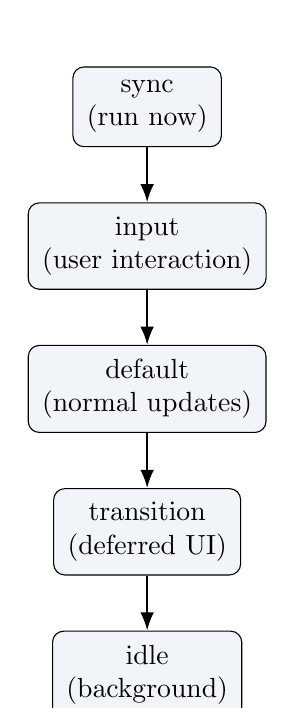
\begin{tikzpicture}[
  node distance=7mm,
  box/.style={draw,rounded corners,fill=RelaxLight,inner sep=5pt,align=center},
  arrow/.style={-Latex,thick}
]
  \node[box] (sync) {sync\\(run now)};
  \node[box, below=of sync] (input) {input\\(user interaction)};
  \node[box, below=of input] (def) {default\\(normal updates)};
  \node[box, below=of def] (trans) {transition\\(deferred UI)};
  \node[box, below=of trans] (idle) {idle\\(background)};

  \draw[arrow] (sync) -- (input);
  \draw[arrow] (input) -- (def);
  \draw[arrow] (def) -- (trans);
  \draw[arrow] (trans) -- (idle);
\end{tikzpicture}
\end{center}

This ordering applies unless aging/deadline promotion temporarily pushes work upward.

\subsection{What is a lane in practice?}

Lanes are not preemption.
They’re an ordering and continuation policy:

\begin{itemize}
  \item tasks run to completion one-by-one
  \item lane selection chooses which queue head runs next
  \item aging/deadlines can temporarily override lane order via promotion
\end{itemize}

\subsection{The sync lane}

A \texttt{sync} task is special: \texttt{schedule('sync', ...)} triggers an immediate flush.

In \texttt{schedule()}:

\begin{itemize}
  \item the task is still enqueued
  \item then the scheduler calls \texttt{flush(\{ budgetMs: Infinity \})}
\end{itemize}

This gives a "run now" lane while still reusing the same task machinery.

\paragraph{Why still enqueue sync tasks?}

Because determinism still matters.
Enqueueing before flushing means sync work still participates in the same stable ordering rules if multiple sync tasks are scheduled.

\section{Flush strategies: how work gets a time slice}

The scheduler accepts \texttt{requestFlush(cb)} in its options.
If you don't provide one, it uses \texttt{createRequestFlush('timeout')}.

\subsection{createRequestFlush(strategy)}

\texttt{createRequestFlush()} supports:

\begin{itemize}
  \item \texttt{'timeout'} (universal fallback): \texttt{setTimeout(cb, 0)}
  \item \texttt{'messageChannel'}: uses \texttt{MessageChannel} if available
  \item \texttt{'raf'}: uses \texttt{requestAnimationFrame} if available
\end{itemize}

Specs in \texttt{runtime/\_\_tests\_\_/scheduler.test.ts} cover:

\begin{itemize}
  \item \texttt{createRequestFlush(messageChannel) uses MessageChannel when available}
  \item \texttt{createRequestFlush(raf) uses requestAnimationFrame when available}
\end{itemize}

\subsection{createBrowserScheduler() convenience}

\texttt{createBrowserScheduler({ strategy })} is a wrapper that wires the chosen strategy into \texttt{requestFlush}.

Spec: \texttt{createBrowserScheduler wires a strategy into requestFlush (smoke)}.

\paragraph{Why these strategies exist}

The scheduler is designed to be embeddable:

\begin{itemize}
  \item in Node-like environments (\texttt{setTimeout})
  \item in browsers where \texttt{MessageChannel} is often lower-latency than timeouts
  \item in UIs where \texttt{requestAnimationFrame} aligns work with the next frame
\end{itemize}

\section{Deterministic ordering inside a lane}

Within a lane, tasks are sorted with explicit tie-breakers:

\begin{enumerate}
  \item earlier \texttt{deadline}
  \item earlier \texttt{timestamp}
  \item lower \texttt{id}
\end{enumerate}

This ordering is implemented by \texttt{sortQueueInLane()}:

\begin{verbatim}
q.sort((a, b) => (a.deadline - b.deadline)
  || (a.timestamp - b.timestamp)
  || (a.id - b.id))
\end{verbatim}

Spec: \texttt{orders tasks within a lane by explicit deadline (then timestamp/id)}.

\subsection{Where deadlines come from}

If you don't provide an explicit \texttt{deadline}, \texttt{schedule()} computes:

\begin{verbatim}
deadline = timestamp + budgetMs
\end{verbatim}

So tasks with smaller budgets naturally get earlier deadlines and bubble forward within their lane.
This is a useful ``do small things first'' heuristic that is still deterministic.

\subsection{Three tie-breakers, one guarantee (and why we need all three)}

It’s tempting to think only deadlines matter, but the scheduler needs a \emph{total} ordering to avoid accidental nondeterminism.
Inside a single lane, two tasks can easily share a deadline (same budget) and timestamp (scheduled in the same tick).
The created \texttt{id} is the final ``stable sort'' key.

The guarantee we want is:

\begin{quote}
If you schedule the same tasks in the same order, you will flush them in the same order.
\end{quote}

This is why the implementation stores \texttt{id} and sorts by \texttt{(deadline, timestamp, id)}.

\section{Budgets: splitting work over multiple flushes}

There are two different "budget" knobs:

\begin{itemize}
  \item \texttt{defaultBudgetMs}: the per-task budget used to compute default \texttt{deadline} and default \texttt{budgetMs}
  \item \texttt{frameBudgetMs}: a global cap for \emph{scheduled flush loops}
\end{itemize}

\subsection{What flush(budgetMs) does}

\texttt{flush(\{ budgetMs \})}:

\begin{itemize}
  \item emits devtools events \texttt{flushStart} and \texttt{flushEnd}
  \item runs tasks in priority order until:
    \begin{itemize}
      \item queues are empty, or
      \item elapsed time exceeds \texttt{budgetMs}
    \end{itemize}
  \item if budget is exceeded \emph{and} work remains, it schedules a continuation flush
\end{itemize}

Specs:

\begin{itemize}
  \item \texttt{budget enforcement: flush splits work across multiple flush calls when budget is tight}
  \item \texttt{setFrameBudget caps the budget used by scheduled flushes}
\end{itemize}

\subsection*{Diagram: the flush loop (budgeted work)}

\begin{center}
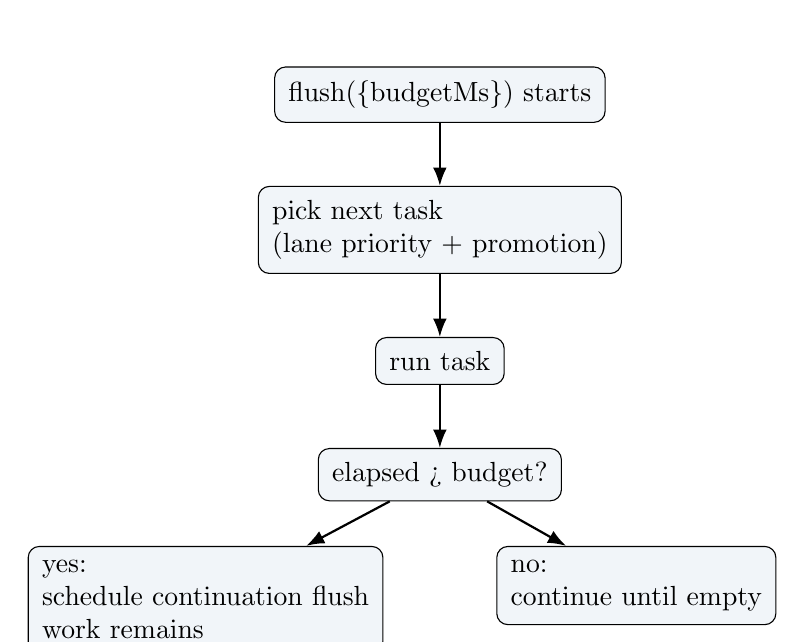
\begin{tikzpicture}[
  node distance=8mm,
  box/.style={draw,rounded corners,fill=RelaxLight,inner sep=5pt,align=left},
  arrow/.style={-Latex,thick}
]
  \node[box] (start) {flush(\{budgetMs\}) starts};
  \node[box, below=of start] (pick) {pick next task\\(lane priority + promotion)};
  \node[box, below=of pick] (run) {run task};
  \node[box, below=of run] (check) {elapsed > budget?};
  \node[box, below left=of check, xshift=14mm] (cont) {yes:\\schedule continuation flush\\work remains};
  \node[box, below right=of check, xshift=-14mm] (done) {no:\\continue until empty};

  \draw[arrow] (start) -- (pick);
  \draw[arrow] (pick) -- (run);
  \draw[arrow] (run) -- (check);
  \draw[arrow] (check) -- (cont);
  \draw[arrow] (check) -- (done);
\end{tikzpicture}
\end{center}

\subsection{setFrameBudget(ms)}

Even if tasks provide their own budgets, scheduled flushes are capped by \texttt{frameBudgetMs}.

The spec demonstrates this by setting \texttt{frameBudgetMs = 1} and scheduling tasks that each consume \texttt{2ms}; only one task runs per flush, and the second flush runs the remainder.

\subsection{Frame budget versus task budget (important distinction)}

In \texttt{runtime/scheduler.ts}, \texttt{budgetMs} is stored on each task, but it isn't directly used by \texttt{flush()}.
Instead:

\begin{itemize}
  \item \textbf{task budget} influences default deadlines (and therefore ordering)
  \item \textbf{flush budget} (\texttt{flush(\{budgetMs\})} or \texttt{frameBudgetMs}) limits how long the flush loop runs before continuation is scheduled
\end{itemize}

The test suite focuses on flush budgets because those directly affect responsiveness.

\subsection{Walkthrough: tight budget slicing (mapping a test to code)}

Read the spec named \texttt{budget enforcement: flush splits work across multiple flush calls when budget is tight}.
It schedules three tasks; each task increments a manual clock by 3ms.
Then it runs two flush calls with \texttt{budgetMs = 5}.

The implementation in \texttt{runtime/scheduler.ts} does exactly this:

\begin{enumerate}
  \item stores \texttt{start = now()}
  \item runs one task at a time
  \item recomputes \texttt{elapsed = now() - start}
  \item stops once \texttt{elapsed >= budgetMs}
\end{enumerate}

So with 3ms per task:

\begin{itemize}
  \item task 1 leaves us at 3ms (still under 5ms)
  \item task 2 leaves us at 6ms (over budget) \textrightarrow stop and continue later
  \item task 3 remains queued for the next flush
\end{itemize}

This is "cooperative scheduling": tasks cooperate by being small and letting the runtime yield.
If you want more intuition about why we care, the web performance RAIL model is a good framing for latency budgets:
\href{https://web.dev/rail/}{https://web.dev/rail/}.

\subsection{Timeline example: lane priority, aging, and budget all at once}

The trickiest behavior is when \emph{multiple policies apply}: lane order, promotion, and a flush budget.
Let's walk a concrete timeline using the same concepts as \texttt{makeManualScheduler()} in the tests.

Assume:

\begin{itemize}
  \item \texttt{AGING\_MS = 250}
  \item \texttt{frameBudgetMs = 5}
  \item each task costs \texttt{3ms} (it advances the manual clock)
\end{itemize}

We schedule:

\begin{lstlisting}[language=JavaScript]
// T = 0
scheduler.schedule('idle', () => tick(3))

// time passes; the idle head is now "old"
tick(300)

// scheduling default work ensures a flush is scheduled
scheduler.schedule('default', () => tick(3))
\end{lstlisting}

Now what happens during \texttt{flush()}?

\begin{enumerate}
  \item \textbf{Promotion step}: before lane selection, the scheduler checks the idle head.
        It has aged, so it is promoted to \texttt{transition}.
  \item \textbf{Lane selection}: the scheduler picks the highest-priority non-empty lane.
        At this point we have \texttt{default} (new) and \texttt{transition} (promoted).
        The lane order says \texttt{default} wins.
  \item \textbf{But why do tests show idle can run first?} Because the implementation promotes by \emph{moving the task to a higher-priority lane} before selection.
        Across repeated picks (and depending on the exact mix in queues), promotion can change which lane is "non-empty" at the top.
\end{enumerate}

The important lesson isn't the specific interleaving---it's that the promotion rule is deterministic and testable.
When you change the policy, the tests will immediately surface the new ordering.

\subsection{Edge cases to keep in mind}

When you build APIs on top of this scheduler (signals, blocks), three edge cases matter:

\begin{itemize}
  \item \textbf{Re-entrancy}: a running task may schedule more tasks. Determinism requires those tasks get consistent timestamps/ids.
  \item \textbf{Budget 0}: \texttt{setFrameBudget(0)} makes scheduled flushes yield aggressively. That's allowed, but it can create many continuation flushes.
  \item \textbf{Clock source}: using \texttt{performance.now()} in production versus a manual clock in tests is fine, but it means ``timestamp equality'' is common only in tests.
\end{itemize}

\section{Deadlines and aging: starvation prevention via promotion}

HRBR's scheduler includes an aging/promotion mechanism.

In the implementation:

\begin{itemize}
  \item \texttt{AGING\_MS = 250}
  \item lanes eligible for promotion checks: \texttt{idle}, \texttt{transition}, \texttt{default}
  \item promotion moves one step toward higher priority:
    \texttt{idle -> transition -> default -> input}
\end{itemize}

Promotion runs \emph{before} picking the next task, and it only considers the \textbf{queue head} in each lane.

\subsection*{Diagram: promotion ladder}

\begin{center}
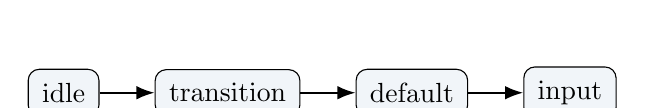
\begin{tikzpicture}[
  node distance=7mm,
  box/.style={draw,rounded corners,fill=RelaxLight,inner sep=5pt,align=center},
  arrow/.style={-Latex,thick}
]
  \node[box] (idle) {idle};
  \node[box, right=of idle] (trans) {transition};
  \node[box, right=of trans] (def) {default};
  \node[box, right=of def] (input) {input};
  \draw[arrow] (idle) -- (trans);
  \draw[arrow] (trans) -- (def);
  \draw[arrow] (def) -- (input);
\end{tikzpicture}
\end{center}

The scheduler promotes a task when it's overdue (deadline reached) or old (aging threshold). This is the mechanism behind the starvation-prevention specs.

A task is promoted if:

\begin{itemize}
  \item it is overdue: \texttt{now() >= head.deadline}, or
  \item it is old: \texttt{now() - head.timestamp > AGING\_MS}
\end{itemize}

Specs:

\begin{itemize}
  \item \texttt{ages/pushes starving tasks upwards (idle -> transition)}
  \item \texttt{promotes a task when its deadline is reached}
  \item \texttt{starvation prevention: repeated promotions eventually let idle work run even under continuous input load}
\end{itemize}

One subtlety the tests call out:

\begin{quote}
Promotion happens before lane selection, so an aged/overdue idle task can execute before later-scheduled default work.
\end{quote}

This is a deliberate fairness trade-off.

\subsection{Fairness without nondeterminism}

The promotion rule checks only \textbf{queue heads} and promotes at most one task per candidate lane per pick.
That has two benefits:

\begin{itemize}
  \item it's cheap (no scanning the entire queue)
  \item it stays deterministic (the head is a deterministic choice)
\end{itemize}

\subsection{Why promotion checks only queue heads}

The promotion policy is intentionally restricted to heads:

\begin{itemize}
  \item It's \textbf{predictable}: given the same inputs and the same clock, you'll promote the same tasks.
  \item It's \textbf{O(1)} per lane: no scanning and no ``who is most starving'' heuristics.
  \item It preserves within-lane ordering as much as possible.
\end{itemize}

This is a classic engineering trade-off: accept a slightly simplified fairness model to buy determinism and low overhead.

\section{withBudget(): bridging user work and scheduler work}

Real apps do work outside of the scheduler too (rendering, event handlers, parsing).
\texttt{withBudget(budgetMs, fn)} is a helper that:

\begin{itemize}
  \item runs \texttt{fn}
  \item if \texttt{fn} exceeds the budget and tasks remain, it schedules a continuation flush
\end{itemize}

Spec: \texttt{withBudget schedules continuation when user code exhausts budget and tasks remain}.

This is the "be nice to the main thread" glue between imperative work and queued reactive work.

\subsection{A practical use case: big event handler + pending effects}

Imagine an event handler that does some synchronous work (parsing, filtering, sorting) and also triggers signal writes.
Those writes schedule computations, but you still want control: if your handler took too long, queue a flush continuation.

\begin{lstlisting}[language=JavaScript]
import { withBudget } from './runtime'

withBudget(4, () => {
  // expensive user work
  // ... parse, compute, validate ...
  // signals may schedule effects while we do this
})
// if the 4ms budget was exceeded and work is pending,
// the scheduler will ensure another flush is scheduled.
\end{lstlisting}

\subsection{Global helpers in \texttt{runtime/index.ts}}

The runtime also exports shared budgeting helpers that use a module-level global scheduler:

\begin{itemize}
  \item \texttt{withBudget(budgetMs, fn)}
  \item \texttt{setFrameBudget(ms)}
\end{itemize}

This is covered by the smoke test \texttt{runtime withBudget() helper returns the callback result and is callable}.

\section{Devtools and instrumentation hooks}

The scheduler calls \texttt{emitDevtoolsEvent()} (\texttt{runtime/devtools.ts}) when flushing:

\begin{itemize}
  \item \texttt{flushStart}
  \item \texttt{flushEnd\{ durationMs \}}
\end{itemize}

These feed counters like \texttt{flushes} and \texttt{flushTimeMs}.

Signals also emit \texttt{scheduleComputation} events when a computation is scheduled.

(We’ll use these counters later when measuring block update costs.)

\subsection{Why ``events + counters'' is a good runtime pattern}

Two competing goals exist:

\begin{itemize}
  \item keep the runtime fast (no heavy logging)
  \item make the runtime observable (so you can measure and debug)
\end{itemize}

The implementation in \texttt{runtime/devtools.ts} uses a tiny event stream plus aggregated counters.
That means you can do ``always-on'' cheap counting (flush count/time) and keep deeper instrumentation behind a toggle.

\section{Walking the tests: what they prove}

The runtime scheduler suite is unusually readable because it uses a manual clock and a manual flush queue.
That makes time and continuation behavior deterministic.

\subsection{Core semantics (\texttt{runtime/\_\_tests\_\_/scheduler.test.ts})}

\begin{description}
  \item[runs tasks by lane priority] Proves the lane order and that \texttt{sync} executes immediately.
  \item[orders tasks within a lane by explicit deadline] Proves the sort tie-breakers inside a lane.
  \item[respects budget and continues in a later flush] Proves a scheduled flush loop may stop early and reschedule continuation.
  \item[budget enforcement: flush splits work] Proves deterministic time slicing under a small budget.
  \item[setFrameBudget caps scheduled flush budget] Proves continuation flushes use \texttt{frameBudgetMs} as a cap.
  \item[ages/pushes starving tasks upwards] Proves age-based promotion and the fairness trade-off (promoted work can run before later default work).
  \item[promotes a task when its deadline is reached] Proves deadline-based promotion independent of age.
  \item[starvation prevention under input load] Proves repeated promotions eventually allow idle work to run.
  \item[createRequestFlush(messageChannel/raf)] Proves strategy selection uses platform APIs when present.
  \item[createBrowserScheduler smoke] Proves wiring strategy into \texttt{requestFlush}.
\end{description}

\subsection{How to read these tests like a spec}

The tests are valuable because they remove nondeterminism from time.
The helper \texttt{makeManualScheduler()} provides:

\begin{itemize}
  \item a manual clock: \texttt{tick(ms)}
  \item a list of pending flush callbacks: \texttt{runNextFlush()} / \texttt{runAllFlushes()}
\end{itemize}

So when you see an assertion like \texttt{expect(order).toEqual([...])}, you're basically reading the scheduler's language definition.

\section{Online resources}

\begin{itemize}
  \item MDN: \href{https://developer.mozilla.org/en-US/docs/Web/API/MessageChannel}{\texttt{MessageChannel}}
  \item MDN: \href{https://developer.mozilla.org/en-US/docs/Web/API/window/requestAnimationFrame}{\texttt{requestAnimationFrame}}
  \item MDN: \href{https://developer.mozilla.org/en-US/docs/Web/JavaScript/Event_loop}{Event loop (tasks, microtasks)}
  \item React (conceptual parallel): \href{https://react.dev/learn/render-and-commit}{Render/commit (scheduling intuition)}
  \item Cooperative background work (conceptual): \href{https://developers.google.com/web/updates/2015/08/using-requestidlecallback}{\texttt{requestIdleCallback}}
\end{itemize}

\section{Takeaways}

\begin{itemize}
  \item Lanes provide a small, explicit latency model with a deterministic priority order.
  \item Each lane is internally sorted by deadline, then timestamp, then id.
  \item Budgeting is enforced at flush time to time-slice work.
  \item Aging/promotion makes starvation unlikely without making scheduling non-deterministic.
  \item \texttt{withBudget} lets user code cooperate with the scheduler.
\end{itemize}

\chapter{HRBR Blocks: Template + Slots (the Compiled Fast Path)}

Chapters 12 and 13 gave us two halves of a reactive UI runtime:

\begin{itemize}
  \item \textbf{Signals} decide \emph{what} values changed.
  \item \textbf{Scheduler lanes} decide \emph{when} to apply work.
\end{itemize}

Blocks are the third half: they decide \emph{how} to touch the DOM.

A \textbf{block} is the "fast DOM" path: it describes a stable DOM template and a set of precise write locations (slots). Updates become \emph{O(k)} slot writes instead of building a VDOM tree and diffing children.

This chapter is grounded in:

\begin{itemize}
  \item Implementation: \texttt{runtime/block.ts}
  \item Specs: \texttt{runtime/\_\_tests\_\_/block.test.ts}
  \item Slot matrix: \texttt{runtime/\_\_tests\_\_/block-slot-matrix.test.ts}
  \item Input controls: \texttt{runtime/\_\_tests\_\_/block-input-controls.test.ts}
  \item Disposal correctness: \texttt{runtime/\_\_tests\_\_/block-disposal.test.ts}
\end{itemize}

\section{A tiny contract (what a block guarantees)}

Treat this as the “promise” the runtime makes to compiled code:

\begin{enumerate}
  \item \textbf{Single stable root:} \texttt{templateHTML} must produce exactly one root element, which is cloned and appended to the host.
  \item \textbf{Exact addressing:} each slot points to a node using a \texttt{path: number[]} walk over \texttt{childNodes} indices.
  \item \textbf{Specialized patching:} slot kinds are patched by small, explicit routines (text/attr/prop/class/style/event).
  \item \textbf{No needless DOM writes:} redundant values are skipped via \texttt{Object.is}.
  \item \textbf{Safe lifecycle:} \texttt{destroy()} is idempotent, removes listeners, and after destroy further \texttt{update()} calls are ignored.
\end{enumerate}

\section{Block vocabulary}

\subsection{TemplateHTML}

A block definition includes a \texttt{templateHTML: string}.
This must produce exactly one root element.

Implementation detail: \texttt{parseTemplate(templateHTML)} uses a \texttt{<template>} element and asserts:

\begin{quote}
\texttt{templateHTML must have a single root element}
\end{quote}

The implementation is intentionally strict:

\begin{itemize}
  \item it does \texttt{templateHTML.trim()} before parsing
  \item it reads \texttt{tpl.content.firstElementChild}
  \item it asserts non-null and returns the root element
\end{itemize}

This makes “multiple root nodes” a loud error, which is what you want for compiled templates.

\subsection{Slot}

A \textbf{slot} is a metadata record describing \emph{where} and \emph{how} to write a dynamic value into a template instance.

Slots are keyed by string (slot key) and come in these kinds:

\begin{itemize}
  \item \texttt{text}: write to a Text node
  \item \texttt{attr}: set/remove attributes
  \item \texttt{prop}: set DOM properties
  \item \texttt{class}: write \texttt{class} attribute
  \item \texttt{style}: write inline styles
  \item \texttt{event}: bind events once and swap handler references
\end{itemize}

Each slot includes a \texttt{path: number[]} which is a \textbf{childNodes index walk} from the template root.

Two practical consequences:

\begin{itemize}
  \item \texttt{childNodes} counts text nodes and comments, so whitespace in templates matters.
  \item Slot paths are best generated by a compiler that controls the template serialization.
\end{itemize}

\section{Why paths (and not querySelector)?}

Paths are the “compiled fast path” address:

\begin{itemize}
  \item they’re \emph{exact} (no ambiguities)
  \item they’re cheap (depth walk, no subtree scan)
  \item they enable prefix caching across multiple slots
\end{itemize}

\section{The public API (surface area)}

The core exports in \texttt{runtime/block.ts} are:

\begin{itemize}
  \item \texttt{defineBlock(def)}: identity helper for typing and readability
  \item \texttt{mountBlock(def, host, initialValues?, options?) -> MountedBlock}
  \item \texttt{mountCompiledBlock(def, host, compiledSlots, options?) -> MountedBlock \& \{ dispose() \}}
  \item \texttt{mountNestedBlock(parent, slotKey, def, initialValues?)}
  \item \texttt{mountNestedFallback(parent, slotKey, mount)}
  \item \texttt{resolvePath(root, path)} and \texttt{resolvePathCached(root, path, slotKey, dev?)}
\end{itemize}

Reading guide:

\begin{itemize}
  \item \texttt{mountBlock} is the non-reactive primitive (mount + \texttt{update}).
  \item \texttt{mountCompiledBlock} wires signals into \texttt{update} with effects and the HRBR scheduler.
  \item \texttt{mountNestedBlock}/\texttt{mountNestedFallback} are the structural escape hatches.
\end{itemize}

\section{defineBlock(): the type boundary}

	exttt{defineBlock(def)} doesn’t transform input. It exists so "compiled" code can be explicit and type-safe.

In \texttt{runtime/block.ts}, it is literally an identity function:

\begin{quote}
	exttt{export function defineBlock(def: BlockDef): BlockDef \{ return def \}}
\end{quote}

That sounds trivial, but it creates a clean “compiler boundary” and a stable type surface.

Tests use it in every case:

\begin{verbatim}
const block = defineBlock({ templateHTML: ..., slots: ... })
\end{verbatim}

\section{mountBlock(): instantiate template + resolve slot nodes}

\texttt{mountBlock()} does the non-reactive mount:

\begin{enumerate}
  \item parse template HTML into a root element
  \item clone it to create an instance
  \item append instance root to the host
  \item resolve each slot \texttt{path} into a concrete DOM \texttt{Node}
  \item apply \texttt{initialValues} via \texttt{block.update(initialValues)}
\end{enumerate}

The key optimization is “resolve once, write many”: paths are resolved at mount time and stored in \texttt{slotNodes}. Updates never traverse the DOM tree; they dereference and write.

The returned \texttt{MountedBlock} includes:

\begin{itemize}
  \item \texttt{root}: the mounted root element
  \item \texttt{slotNodes}: mapping from slot key to resolved node reference
  \item \texttt{update(values)}: apply slot writes
  \item \texttt{destroy()} / \texttt{dispose()} lifecycle
\end{itemize}

\subsection{Path resolution and caching}

\texttt{resolvePath(root, path)} is the simple implementation.
But \texttt{mountBlock} uses \texttt{resolvePathCached(instanceRoot, path, slotKey, dev)}.

The cache is a \texttt{Map<string, Node>} stored on the instance root as \texttt{\_\_hrbrPathCache}.
Prefixes are stored as dot-joined strings like \texttt{"1.0"}.

The caching algorithm is incremental: as it walks the path, it caches each prefix result (\texttt{"1"}, then \texttt{"1.0"}, etc.). Multiple slots that share a prefix benefit immediately.

Spec: \texttt{mountBlock caches repeated path prefixes across slots}.

\subsection{Dev diagnostics}

When \texttt{options.dev === true}, the assertions include the slot key in the error.

Spec: \texttt{dev diagnostics: mountBlock includes slot key in invalid path errors (dev mode)}.

\section{update(values): slot patching rules}

The update loop iterates over provided keys only. If a key doesn’t exist in \texttt{def.slots}, it is ignored.

Two important performance rules:

\begin{itemize}
  \item The block stores \texttt{prevValues[key]} and skips redundant writes using \texttt{Object.is}.
  \item It emits a devtools event \texttt{slotWrite} for each actual write.
\end{itemize}

The use of \texttt{Object.is} is deliberate: it treats \texttt{NaN} as equal to itself and provides a cheap “same reference” check for objects (like style objects or class arrays).

Spec: \texttt{skips redundant writes for unchanged values (text + attr)}.

\subsection{text slots}

Text slots must resolve to a real Text node. The runtime asserts:

\begin{quote}
\texttt{slot 'x' expected a Text node}
\end{quote}

Writes use \texttt{Text.nodeValue} and normalize nullish values to the empty string.

Spec: \texttt{mounts a template and updates text slots by path}.

\subsection{attr slots (including boolean attributes and SVG xlink)}

Attribute writes route through \texttt{setAttr(el, name, next)}:

\begin{itemize}
  \item \texttt{null | false} removes the attribute
  \item boolean-ish attributes are present/absent (set to empty string)
  \item SVG \texttt{xlink:*} attributes use \texttt{setAttributeNS}
\end{itemize}

Implementation notes:

\begin{itemize}
  \item SVG detection uses \texttt{namespaceURI} (not \texttt{instanceof SVGElement}) for broader runtime compatibility.
  \item Boolean attribute names are normalized (\texttt{readOnly} maps to \texttt{readonly}).
\end{itemize}

Specs:

\begin{itemize}
  \item \texttt{updates attribute slots by path}
  \item \texttt{treats boolean attributes as present/absent (attr slots)}
  \item \texttt{sets xlink:* attributes with the xlink namespace on SVG elements}
\end{itemize}

\subsection{prop slots (input correctness)}

Property slots route through \texttt{setProp(el, name, next)}.

Special-case correctness for inputs:

\begin{itemize}
  \item \texttt{value}: written as a string property, nullish clears to \texttt{""}
  \item \texttt{checked}: written as boolean
\end{itemize}

This matches standard controlled-input behavior: writing to properties updates the live control state, while attributes can drift.

Specs:

\begin{itemize}
  \item \texttt{updates property slots by path}
  \item \texttt{updates input value/checked via property semantics for prop slots}
  \item input control suite in \texttt{block-input-controls.test.ts}
\end{itemize}

\subsection{class slots}

Class slots write the \texttt{class} attribute:

\begin{itemize}
  \item \texttt{null | false} removes the attribute
  \item arrays are joined with spaces after filtering falsy values
  \item otherwise coerced to string
\end{itemize}

\subsection{style slots}

Style slots accept:

\begin{itemize}
  \item \texttt{null | false}: remove whole style attribute
  \item string: set \texttt{style} attribute directly
  \item object: per-key \texttt{style.setProperty} / \texttt{removeProperty}
\end{itemize}

This small matrix is validated by \texttt{block-slot-matrix.test.ts}.

\subsection{event slots: bind once, swap handler}

Event slots are designed to avoid listener leaks and avoid churn:

\begin{itemize}
  \item the first time a slot is set, the runtime binds a stable listener function
  \item the listener reads \texttt{rec.current} to find the latest handler
  \item updates replace \texttt{rec.current} without re-binding
  \item destroying the block removes the listener
\end{itemize}

Specs:

\begin{itemize}
  \item \texttt{supports event slots: binds once and updates handler without leaking listeners}
  \item \texttt{destroy removes event listeners (no further handler calls)}
  \item \texttt{skips redundant event listener churn when handler identity is unchanged}
\end{itemize}

\subsubsection{Matching Relax VDOM semantics: hostComponent binding}

\texttt{mountBlock(..., \{ hostComponent \})} optionally calls handlers with \texttt{this === hostComponent}, matching Chapter 7’s event binding behavior in the VDOM runtime.

\section{Lifecycle: destroy vs dispose, and idempotency}

\texttt{mountBlock} is not reactive by itself, so \texttt{dispose()} is just an alias for \texttt{destroy()}.

\texttt{destroy()} is idempotent:

\begin{itemize}
  \item it guards with a \texttt{destroyed} flag
  \item it destroys composed children
  \item it removes event listeners
  \item it removes the block root from the DOM
\end{itemize}

After \texttt{destroy()}, \texttt{update()} becomes a no-op (guarded by the same \texttt{destroyed} flag). That prevents stale scheduled work from mutating detached DOM.

Specs:

\begin{itemize}
  \item \texttt{destroy is idempotent even with event slots and children}
  \item \texttt{lifecycle: destroy() is idempotent and prevents further updates}
\end{itemize}

\section{mountCompiledBlock(): wiring signals to slot writes}

\texttt{mountCompiledBlock} is the bridge between the reactive graph and the block DOM writer.

Input: \texttt{CompiledSlot[]} where each entry is:

\begin{verbatim}
{ key: string, read: () => unknown }
\end{verbatim}

\textbf{Important:} \texttt{read()} can access signals; that’s how dependency tracking happens.

Mechanism:

\begin{itemize}
  \item compute initial values by running each \texttt{read()}
  \item mount a non-reactive block with those initial values
  \item create one \texttt{createEffect()} per compiled slot
  \item coalesce multiple invalidations into a single scheduled \texttt{flushPending}
  \item execute \texttt{block.update(values)} inside \texttt{batch()} to keep effects consistent
\end{itemize}

The coalescing logic (\texttt{pending} + \texttt{scheduled} flag) is the performance heart: many effects can invalidate in one turn, but only one scheduled task drains \texttt{pending} and commits to the DOM.

Scheduling goes through the deterministic lane scheduler from Chapter 13:

\begin{quote}
	exttt{scheduler.schedule(lane, flushPending)}
\end{quote}

Spec: \texttt{changing a signal updates only the intended DOM node (mountCompiledBlock)}.

That test also checks identity stability:

\begin{itemize}
  \item the static DOM elements are not recreated
  \item text node identity remains stable; only \texttt{nodeValue} changes
\end{itemize}

Spec: \texttt{mounting does not recreate static DOM during updates}.

\subsection{Disposal stops reactive updates}

\texttt{mountCompiledBlock} returns a \texttt{dispose()} method that:

\begin{itemize}
  \item disposes all effects
  \item destroys the block DOM
  \item is idempotent
\end{itemize}

Specs:

\begin{itemize}
  \item \texttt{mountCompiledBlock.dispose stops reactive updates and removes DOM}
  \item \texttt{lifecycle: mountCompiledBlock.dispose() stops reactive updates and is idempotent}
\end{itemize}

\section{Composition: nested blocks and fallback regions}

Blocks are stable and fast, but real UIs still need dynamic structure.
\texttt{runtime/block.ts} provides two small composition helpers:

\begin{itemize}
  \item \texttt{mountNestedBlock(parent, slotKey, def)}: mount a child block into an Element slot
  \item \texttt{mountNestedFallback(parent, slotKey, mount)}: mount a structural fallback region into an Element slot
\end{itemize}

Both helpers:

\begin{itemize}
  \item clear the host element’s existing children
  \item mount into it
  \item register a child destructor so destroying the parent destroys the child
\end{itemize}

Specs in \texttt{runtime/\_\_tests\_\_/block.test.ts}:

\begin{itemize}
  \item \texttt{block composition: can mount a nested block ... and destroys it with parent}
  \item \texttt{block composition: can mount a nested fallback region ... and disposes it with parent}
\end{itemize}

This is HRBR's interop story:

\begin{quote}
Compiled stable subtrees use blocks; dynamic subtrees route to fallback reconciliation.
\end{quote}

Implementation detail: composition is tracked with a small internal child registry.
	exttt{mountBlock} exposes an internal \texttt{\_\_hrbrTrackChild} function, and the composition helpers use it to register child destroyers so teardown order is correct.

\section{Walking the tests (the executable spec)}

\subsection{\texttt{runtime/\_\_tests\_\_/block.test.ts}}

This test file locks down the baseline behavior of each slot type and of the compiled/reactive mount.

\begin{itemize}
  \item \textbf{text slots:} the slot must resolve to a real Text node; updates rewrite \texttt{nodeValue}; destroy removes DOM.
  \item \textbf{attr slots:} \texttt{null} removes the attribute.
  \item \textbf{prop slots:} input \texttt{value} is updated via property semantics.
  \item \textbf{class/style:} \texttt{null} removes attrs, arrays join for class, style objects set properties.
  \item \textbf{event slots:} click once, swap handler, click again; after \texttt{destroy()} clicks do nothing.
  \item \textbf{boolean attributes:} present/absent behavior is asserted with \texttt{disabled}.
  \item \textbf{SVG xlink:} uses \texttt{getAttributeNS} to validate namespace behavior.
  \item \textbf{path caching:} asserts \texttt{\_\_hrbrPathCache} contains prefix keys (e.g. \texttt{"0"}, \texttt{"0.0"}).
  \item \textbf{dev diagnostics:} invalid path errors include the slot key in dev mode.
  \item \textbf{mountCompiledBlock:} changing one signal updates only its text node, and node identity is stable across updates.
\end{itemize}

\subsection{\texttt{runtime/\_\_tests\_\_/block-slot-matrix.test.ts}}

This is a matrix-style smoke test that mounts one template with \textbf{all slot kinds} and asserts both initial values and updated values, including event swapping.

\subsection{\texttt{runtime/\_\_tests\_\_/block-input-controls.test.ts}}

This suite documents the intended controlled-input semantics for \texttt{value} and \texttt{checked} when patched as properties.
It also includes a note about radio group behavior in jsdom.

\subsection{\texttt{runtime/\_\_tests\_\_/block-disposal.test.ts}}

This suite locks down lifecycle safety:

\begin{itemize}
  \item \texttt{destroy()} removes event listeners (clicking a detached element must not call handlers).
  \item \texttt{destroy()} is idempotent.
  \item \texttt{mountCompiledBlock.dispose()} stops reactive updates and removes DOM permanently.
\end{itemize}

\section{Online resources}

\begin{itemize}
  \item \href{https://developer.mozilla.org/en-US/docs/Web/HTML/Element/template}{MDN: \texttt{<template>}} (template parsing and cloning)
  \item \href{https://developer.mozilla.org/en-US/docs/Web/API/Node/childNodes}{MDN: \texttt{Node.childNodes}} (why paths include text/comment nodes)
  \item \href{https://developer.mozilla.org/en-US/docs/Web/API/EventTarget/addEventListener}{MDN: \texttt{addEventListener}} (listener identity + removal)
  \item \href{https://developer.mozilla.org/en-US/docs/Web/API/HTMLInputElement}{MDN: \texttt{HTMLInputElement}} (property semantics for \texttt{value} and \texttt{checked})
  \item \href{https://developer.mozilla.org/en-US/docs/Web/SVG/Attribute/xlink:href}{MDN: \texttt{xlink:href}} (SVG namespaced attribute background)
  \item \href{https://svelte.dev/blog/virtual-dom-is-pure-overhead}{Svelte: “Virtual DOM is pure overhead”} (compiler-driven DOM updates intuition)
\end{itemize}

\section{Takeaways}

\begin{itemize}
  \item Blocks are "template + slots": a stable DOM instance plus precise write locations.
  \item Slot patching is specialized per kind, with correctness for input controls and SVG namespaces.
  \item Updates skip redundant writes via \texttt{Object.is}.
  \item Event slots bind once and swap handler references; destroy removes listeners.
  \item \texttt{mountCompiledBlock} wires signals to slots and coalesces updates into scheduled flushes.
  \item Composition helpers let blocks nest blocks and fallback regions safely.
\end{itemize}

\chapter{Hydration: Attaching HRBR to Server HTML}

\section*{What you'll build}

In this chapter I’ll build a mental model for v1 hydration in Relax, and you’ll learn how to reason about it by reading the real runtime code.
Concretely, you’ll be able to:

\begin{itemize}
  \item take an HTML string that was produced from a BlockDef, insert it into the DOM, and \emph{attach} a live HRBR block to it without rewriting nodes
  \item explain why Relax’s v1 hydration is strict and why that strictness is a feature (not a limitation)
\end{itemize}

\section*{What you'll learn}

\begin{itemize}
  \item The hydration contract: what must match between server HTML and \texttt{templateHTML}
  \item The two safety rails: \texttt{root tag check} and \texttt{slot-path validation}
  \item The cost model: why hydration is cheap when it succeeds, and cheap to bail out when it must
  \item How v1 hydration handles DOM updates (same slot kinds as Chapter~14) and where it differs (events)
\end{itemize}

\section*{Prereqs}

\begin{itemize}
  \item Chapter~14: Blocks, templates, and slots (slot kinds + path addressing)
  \item Chapter~12: Effects and dependency tracking (why \texttt{mountCompiledBlock} works)
\end{itemize}

\section{Why hydration exists (from scratch)}

Hydration is the bridge between two worlds:

\begin{itemize}
  \item The \textbf{server} produced HTML as a string. That’s great for first paint and SEO.
  \item The \textbf{client} needs live behavior: event handlers, reactive updates, and cleanup.
\end{itemize}

If you don’t hydrate, you have only two choices on the client:

\begin{itemize}
  \item \textbf{Remount by recreating DOM} from scratch, which throws away the server’s nodes (and can introduce a visible flash), or
  \item \textbf{Try to patch your way into the server DOM} with a general reconciler, which is powerful but hard to make airtight.
\end{itemize}

Relax HRBR v1 chooses a third option:

\begin{quote}
	extbf{Attach by validating structure and resolving slot node references.} If validation fails, remount.
\end{quote}

This conservative posture is intentional. It makes hydration predictable: the moment we say “hydrated”, we’re also saying the block’s template ABI matches the DOM we’re about to mutate.

\section{The big picture: where hydration sits in HRBR}

A block runtime has a natural relationship with server rendering:

\begin{itemize}
  \item The compiler produces a stable template shape (\texttt{templateHTML}).
  \item The server can render the template to HTML.
  \item The client can \emph{attach} to the existing DOM instead of rebuilding it.
\end{itemize}

In Relax HRBR v1, hydration is deliberately conservative. If anything looks wrong, it bails out and remounts client-side.

\begin{center}
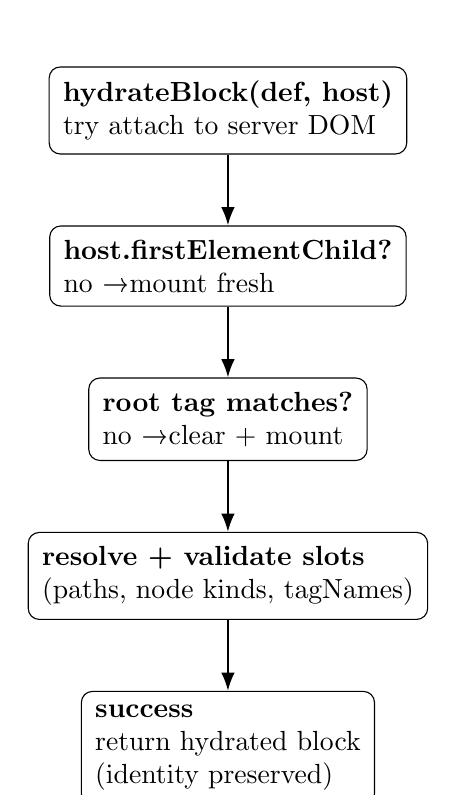
\begin{tikzpicture}[
  node distance=9mm,
  box/.style={draw, rounded corners, align=left, inner sep=5pt},
  arrow/.style={-Latex, thick}
]
\node[box] (start) {\textbf{hydrateBlock(def, host)}\\try attach to server DOM};
\node[box, below=of start] (hasroot) {\textbf{host.firstElementChild?}\\no \textrightarrow mount fresh};
\node[box, below=of hasroot] (rootok) {\textbf{root tag matches?}\\no \textrightarrow clear + mount};
\node[box, below=of rootok] (slots) {\textbf{resolve + validate slots}\\(paths, node kinds, tagNames)};
\node[box, below=of slots] (ok) {\textbf{success}\\return hydrated block\\(identity preserved)};

\draw[arrow] (start) -- (hasroot);
\draw[arrow] (hasroot) -- (rootok);
\draw[arrow] (rootok) -- (slots);
\draw[arrow] (slots) -- (ok);
\end{tikzpicture}
\end{center}

This chapter is grounded in:

\begin{itemize}
  \item \texttt{runtime/hydration.ts} (hydrate implementation)
  \item \texttt{runtime/ssr.ts} (string rendering helper used in tests)
  \item \texttt{runtime/\_\_tests\_\_/hydration.test.ts}
  \item \texttt{runtime/\_\_tests\_\_/ssr.test.ts}
\end{itemize}

\section{A tiny contract (what hydrateBlock promises)}

Hydration is the moment where two worlds meet:

\begin{itemize}
  \item The \textbf{server} produced HTML as a string.
  \item The \textbf{client} wants a live block instance with slot node references.
\end{itemize}

In v1, Relax uses a strict approach that is easy to reason about and hard to get subtly wrong.
You can treat \texttt{hydrateBlock(def, host, initialValues)} as enforcing this contract:

\begin{enumerate}
  \item If there is no DOM to attach to (\texttt{host.firstElementChild == null}), hydration simply mounts a fresh block.
  \item If the root element tag does not match the template’s root tag, hydration clears the host and mounts fresh.
  \item If slot paths resolve to the wrong node types or to the wrong element tag names (compared to the parsed template), hydration clears the host and mounts fresh.
  \item If everything matches, hydration returns a block-like object whose \texttt{root} and \texttt{slotNodes} refer to the server DOM nodes.
\end{enumerate}

The headline design choice is: \textbf{when in doubt, remount}. That makes correctness obvious at the cost of being less clever than incremental/partial hydration systems.

\section{Build it: a minimal end-to-end hydration loop}

I like to teach hydration as a 3-step loop: \textbf{render} \(\rightarrow\) \textbf{attach} \(\rightarrow\) \textbf{update}.

In Relax, the pieces are:

\begin{itemize}
  \item \texttt{renderBlockToString(def, \{ initialValues \})} (SSR helper)
  \item \texttt{host.innerHTML = html}
  \item \texttt{hydrateBlock(def, host, initialValues)} (attach)
  \item optionally: \texttt{mountCompiledBlock(def, host, compiledSlots)} to wire signals/effects (Chapter~14)
\end{itemize}

Here’s the smallest "looks runnable" snippet that matches what the tests demonstrate.

\begin{lstlisting}[language=JavaScript, caption={SSR + hydration + update: the smallest end-to-end loop}]
import { defineBlock, mountCompiledBlock } from './runtime/block'
import { hydrateBlock } from './runtime/hydration'
import { createSignal } from './runtime/signals'
import { renderBlockToString } from './runtime/ssr'

const Counter = defineBlock({
  templateHTML: `<div class="c"><button id="inc">+</button><span id="t"> </span></div>`,
  slots: { value: { kind: 'text', path: [1, 0] } },
})

// "Server" side
const html = renderBlockToString(Counter, { initialValues: { value: 'A' } })

// "Client" side
const host = document.getElementById('host')
host.innerHTML = html

// Attach to existing nodes (no rewrite if markup matches)
const hydrated = hydrateBlock(Counter, host)

// Wire reactive updates on top (optional, but this is the HRBR story)
const [value, setValue] = createSignal('A')
const mounted = mountCompiledBlock(Counter, host, [{ key: 'value', read: () => value() }])

setValue('B')
mounted.update({ value: 'B' })

mounted.dispose()
hydrated.destroy()
\end{lstlisting}

\subsection{Why these steps matter}

\begin{itemize}
  \item \textbf{SSR produces a shape:} If SSR and the template disagree, hydration must not "half attach".
  \item \textbf{Hydration creates references:} the essential output is \texttt{slotNodes[key] = Node}.
  \item \textbf{Updates are the same contract:} a call to \texttt{update(\{ key: value \})} still means “write into slot nodes”.
\end{itemize}

\section{Hydration contract (v1)}

\texttt{hydrateBlock(def, host, initialValues?)} returns a \texttt{HydratedBlock} (type alias of \texttt{MountedBlock}).

Its docstring states three key assumptions:

\begin{enumerate}
  \item \texttt{host} contains exactly one root element matching the template.
  \item Hydration does not mutate DOM; it only resolves slot node references.
  \item On mismatch, hydration bails out and remounts client-side.
\end{enumerate}

This is a strict, "safety first" strategy: it prefers correctness over partial hydration tricks.

It’s also worth noticing what the contract does \emph{not} promise:

\begin{itemize}
  \item It does not try to recover from mismatches by patching individual nodes.
  \item It does not attempt to reconcile text/comment whitespace differences.
  \item It does not do event delegation or partial listener attachment.
\end{itemize}

\section{The fast path: attach without rewriting}

Given server markup like:

\begin{verbatim}
<div><span>A</span></div>
\end{verbatim}

and a matching block definition:

\begin{verbatim}
templateHTML: `<div><span>A</span></div>`
slots: { a: { kind: 'text', path: [0, 0] } }
\end{verbatim}

The hydration algorithm is:

\begin{enumerate}
  \item Read \texttt{serverRoot = host.firstElementChild}.
  \item Validate root tagName against the template (cheap check).
  \item Resolve every slot path against \texttt{serverRoot}.
  \item Validate slot node types, and element tagNames against the template DOM.
  \item Return a \texttt{HydratedBlock} whose \texttt{update()} writes into those resolved nodes.
\end{enumerate}

Two details in \texttt{runtime/hydration.ts} make this efficient:

\begin{itemize}
  \item Root tag validation is a fast regex over \texttt{templateHTML} (\texttt{getRootTagName}). This allows an early bail-out without parsing a template DOM.
  \item Slot resolution is just a \texttt{childNodes} index walk (\texttt{resolvePath}). It’s similar to \texttt{runtime/block.ts}, but hydration keeps its own copy with different error strings.
\end{itemize}

Spec: \texttt{hydrates without rewriting DOM when markup matches}.

What the spec is really asserting is \textbf{node identity preservation}. You can think of hydration as creating a \emph{mapping} from (slot key \(\rightarrow\) DOM node reference) without changing the structure:

\begin{itemize}
  \item before hydration: DOM nodes already exist (from server HTML)
  \item after hydration: we have slot node references pointing at those exact nodes
  \item on update: we mutate those nodes in place
\end{itemize}

\begin{center}
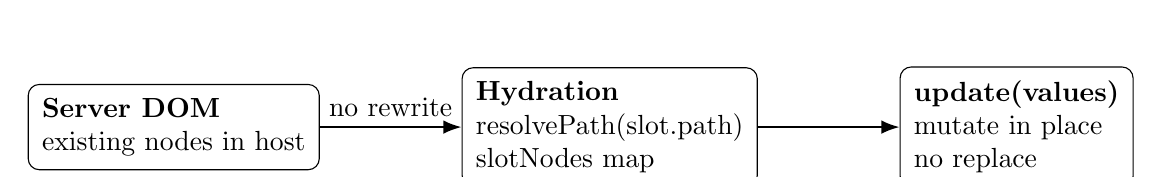
\begin{tikzpicture}[
  node distance=8mm,
  box/.style={draw, rounded corners, align=left, inner sep=5pt},
  arrow/.style={-Latex, thick}
]
\node[box] (server) {\textbf{Server DOM}\\existing nodes in host};
\node[box, right=18mm of server] (refs) {\textbf{Hydration}\\resolvePath(slot.path)\\slotNodes map};
\node[box, right=18mm of refs] (update) {\textbf{update(values)}\\mutate in place\\no replace};

\draw[arrow] (server) -- node[midway, above] {no rewrite} (refs);
\draw[arrow] (refs) -- (update);
\end{tikzpicture}
\end{center}

That test captures node identities before hydration and asserts identity stability after calling \texttt{hydrateBlock}:

\begin{itemize}
  \item same root element
  \item same inner \texttt{<span>}
  \item same text node
\end{itemize}

Then it updates slot values and checks the content changed without replacing nodes.

\section{Mismatch detection: when to bail out}

Hydration needs a mismatch policy. In v1 it is intentionally conservative.

\subsection{Root tag mismatch}

The first check is easy: compare the root tagName.

Implementation: \texttt{getRootTagName(templateHTML)} uses a small regex for the first tag.
If root tags don’t match, hydration does:

\begin{verbatim}
host.innerHTML = ''
return mountBlock(def, host, initialValues)
\end{verbatim}

This is the first key safety property: mismatched DOM never becomes a "half-hydrated" zombie tree. We either attach cleanly or we tear down and replace.

This strict policy gives you an important debugging invariant:

\begin{quote}
If hydration succeeds, later slot writes will never throw because of a missing node or wrong element type (for the validated paths).
\end{quote}

It’s also why HRBR v1 hydration doesn’t try to be clever about whitespace or comment-node drift: the moment your markup generation stops matching the compiler’s structural expectations, hydration deliberately stops and remounts.

Spec: \texttt{mismatch triggers remount for subtree}.

\subsection{Slot path mismatch: element tagName mismatch}

Root tag matching is not enough. You can have the same root element but different internal structure.

The conservative check in \texttt{runtime/hydration.ts} is:

\begin{itemize}
  \item Parse the expected template root into a detached DOM node.
  \item For each non-text slot:
    \begin{itemize}
      \item resolve the same path against the expected template DOM
      \item assert both are Elements
      \item assert \texttt{expected.tagName === actual.tagName}
    \end{itemize}
\end{itemize}

Why compare tag names at slot paths (instead of deep-walking the entire tree)?

\begin{itemize}
  \item Slots are where we will write later, so validating those boundaries catches many mismatches that would otherwise crash later.
  \item It avoids paying for a full tree diff during hydration.
  \item It keeps the rule extremely easy to explain and test.
\end{itemize}

If any assertion fails, hydration catches and bails out with client remount.

Spec: \texttt{slot path element mismatch triggers bailout remount (conservative)}.

\section{Why this design? (tradeoffs, alternatives, and invariants)}

Hydration is an area where it’s easy to ship something that works on your demo and breaks in production.
So I made a deliberate v1 choice: \textbf{strict validation + bailout}.

Here are the tradeoffs I’m optimizing for:

\begin{itemize}
  \item \textbf{Invariant: “hydrated means safe to update.”}
  If hydration returns successfully, the slots you’ll write to later have been validated against the template.

  \item \textbf{Low implementation risk.}
  Partial hydration systems can be correct, but they require more state and more surface area for mismatches.

  \item \textbf{Predictable failure mode.}
  When something is off (wrong tag, wrong path, wrong slot kind), we don’t keep walking a tightrope.
  We clear and remount.
\end{itemize}

Alternatives (all valid, just not v1 Relax):

\begin{itemize}
  \item \textbf{Deep tree diff during hydrate:} robust but expensive and complex.
  \item \textbf{Marker-based hydration:} embed explicit markers in HTML (comment anchors / data attributes). This is a common approach, and it’s likely the direction for a more advanced Relax hydration.
  \item \textbf{Island / partial hydration:} hydrate only interactive regions. Great UX story, more tooling.
\end{itemize}

For a framework-agnostic overview of hydration strategies and tradeoffs, see \href{https://web.dev/rendering-on-the-web/}{https://web.dev/rendering-on-the-web/}.

The test intentionally renders:\\
\texttt{<div><em>X</em></div>}\\
but the template expects:\\
\texttt{<div><span></span></div>}\\
So hydration remounts and you end up with a \texttt{<span>}.

\section{Hydrated update semantics: same slot kinds as mountBlock}

Hydration returns an object that looks like a mounted block:

\begin{itemize}
  \item \texttt{root} is the server root element
  \item \texttt{slotNodes} maps slot keys to resolved DOM nodes
  \item \texttt{update(values)} writes into those nodes
  \item \texttt{destroy()} removes hydrated listeners and removes \texttt{root}
\end{itemize}

The update logic supports the full set of slot kinds:

\begin{itemize}
  \item \texttt{text}: write \texttt{Text.nodeValue}
  \item \texttt{attr}: boolean attribute semantics and SVG xlink namespace
  \item \texttt{prop}: input correctness for \texttt{value} / \texttt{checked}
  \item \texttt{class}: string or array join
  \item \texttt{style}: string or object diff
  \item \texttt{event}: bind event handler(s)
\end{itemize}

Spec: \texttt{hydrates with full slot semantics (event/attr/prop/SVG) without rewriting existing DOM}.

Most of the slot patching logic is a copy of the mount-time block patching rules (Chapter 14), but hydration differs in one important place: event slots.

That test verifies:

\begin{itemize}
  \item DOM identity is preserved for root/button/input/link
  \item clicking calls the hydrated handler
  \item boolean attribute \texttt{hidden} is present
  \item \texttt{checked} property toggles
  \item SVG \texttt{xlink:href} is set in the xlink namespace
\end{itemize}

\subsection{Redundant write skipping}

Hydration tracks \texttt{prevValues} and skips updates when \texttt{Object.is(prev, next)}.
This matches the block runtime’s "skip redundant writes" optimization.

This is a subtle performance win because it also prevents unnecessary listener churn (given hydration’s v1 event strategy below).

\section{Event slots: v1 difference vs mountBlock}

There’s an intentional simplification in hydration:

\begin{itemize}
  \item \texttt{mountBlock} binds once and swaps \texttt{rec.current} (no listener churn).
  \item \texttt{hydrateBlock} removes the previous listener and re-adds on update.
\end{itemize}

You can see this directly in \texttt{runtime/hydration.ts}:

\begin{itemize}
  \item On \texttt{event} updates, it looks up \texttt{listenersByKey[k]}.
  \item If present, it calls \texttt{removeEventListener(prev.type, prev.handler)}.
  \item If the new value is a function, it creates a fresh wrapper handler and calls \texttt{addEventListener(slot.name, handler)}.
\end{itemize}

This is not as optimal as the bind-once approach in \texttt{mountBlock}, but it is still correct and easy to reason about.

Two important correctness notes (easy to miss):

\begin{itemize}
  \item \textbf{Redundant writes matter more with this strategy.} If you didn’t skip redundant writes, a repeated \texttt{update()} could churn listeners (remove+add) even when the handler didn’t change.
  \item \textbf{Destroy must remove hydrated listeners.} Otherwise the host subtree could be detached but still reachable through listener closures.
\end{itemize}

\begin{center}
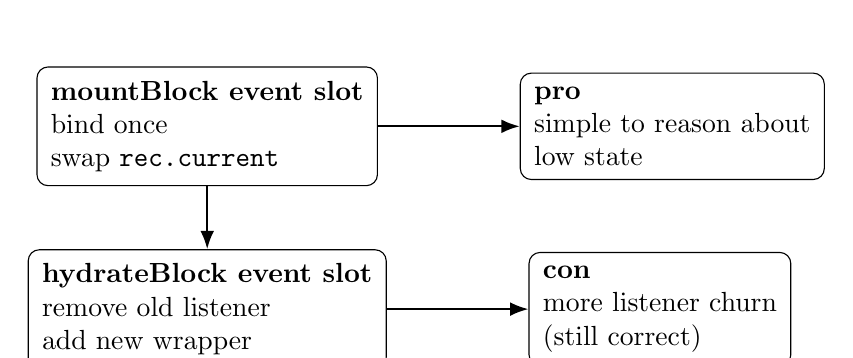
\begin{tikzpicture}[
  node distance=8mm,
  box/.style={draw, rounded corners, align=left, inner sep=5pt},
  arrow/.style={-Latex, thick}
]
\node[box] (mb) {\textbf{mountBlock event slot}\\bind once\\swap \texttt{rec.current}};
\node[box, below=of mb] (hb) {\textbf{hydrateBlock event slot}\\remove old listener\\add new wrapper};
\node[box, right=18mm of mb] (pro) {\textbf{pro}\\simple to reason about\\low state};
\node[box, right=18mm of hb] (con) {\textbf{con}\\more listener churn\\(still correct)};

\draw[arrow] (mb) -- (hb);
\draw[arrow] (mb) -- (pro);
\draw[arrow] (hb) -- (con);
\end{tikzpicture}
\end{center}

The key safety property is lifecycle cleanup: \texttt{destroy()} removes any listeners hydration attached, so even in the “remove + re-add” strategy you don’t leak handlers across updates.

It still avoids leaks because \texttt{destroy()} removes any listeners it attached.

This choice keeps hydration simpler while still correct. If hydration becomes a performance hot spot, it can be refactored to reuse the bind-once strategy.

\section{SSR helper: renderBlockToString()}

\texttt{runtime/ssr.ts} provides a minimal string renderer used mainly for tests.

Contract:

\begin{itemize}
  \item create a detached host element
  \item \texttt{mountBlock(def, host, initialValues)}
  \item read \texttt{host.innerHTML}
  \item destroy the mounted block
\end{itemize}

This is explicitly a v1 teaching tool:

\begin{itemize}
  \item It uses the browser’s DOM implementation to do serialization.
  \item It’s not the kind of streaming SSR engine you’d use in production.
\end{itemize}

But it has an important property: it guarantees that the HTML string shape matches \texttt{mountBlock} semantics, because it’s literally produced by the same code.

Spec: \texttt{renders a block to HTML string, hydrates it, and updates via mountCompiledBlock}.

This gives a full lifecycle demo:

\begin{enumerate}
  \item render HTML string from a block
  \item insert it into the document
  \item hydrate it without rewriting
  \item mount a compiled block on top of the hydrated DOM and update via signals
\end{enumerate}

\section{Takeaways}

\begin{itemize}
  \item Hydration v1 is conservative: it validates structure and bails out on mismatch.
  \item When markup matches, hydration preserves DOM identity (no rewrites).
  \item Hydrated updates support the full slot matrix (text/attr/prop/class/style/event + SVG xlink).
  \item SSR v1 uses the DOM to produce strings for tests; it’s simple and correct, not optimized.
\end{itemize}

\section{Walking the tests (the executable spec)}

Hydration and SSR are notoriously easy to get "mostly right" and still ship broken edge cases.
Relax locks down the v1 behavior with two test files.

\subsection{\texttt{runtime/\_\_tests\_\_/hydration.test.ts}}

This suite defines the hydration safety model.

\begin{itemize}
  \item \textbf{hydrates without rewriting DOM when markup matches}
  captures \texttt{root/span/text} node identities before hydration, hydrates with an initial value, and asserts:
  \begin{itemize}
    \item the same elements/text nodes are still present (identity preserved)
    \item only the content changes
  \end{itemize}

  \item \textbf{hydrates with full slot semantics (event/attr/prop/SVG) without rewriting existing DOM}
  verifies the “slot matrix” works even when DOM is pre-existing:
  \begin{itemize}
    \item event handler is attached and called
    \item boolean-ish attr (\texttt{hidden}) is present
    \item \texttt{checked} is set as a property
    \item SVG \texttt{xlink:href} is set in the xlink namespace
  \end{itemize}

  \item \textbf{mismatch triggers remount for subtree}
  uses the wrong root tag (\texttt{<section>}) and asserts hydration replaces the entire subtree.

  \item \textbf{slot path element mismatch triggers bailout remount (conservative)}
  uses the same root tag but the wrong inner tag at a slot path (\texttt{<em>} vs expected \texttt{<span>}).
  The test asserts that hydration bails out and remounts so the template structure is restored.
\end{itemize}

\subsection{\texttt{runtime/\_\_tests\_\_/ssr.test.ts}}

This test is a full lifecycle demo "in miniature":

\begin{enumerate}
  \item \textbf{render} a block to an HTML string via \texttt{renderBlockToString}
  \item insert the HTML into a host
  \item \textbf{hydrate} without changing root/text node identities
  \item \textbf{mountCompiledBlock} to wire signals and update the hydrated DOM
\end{enumerate}

It’s intentionally pragmatic: rather than relying on timing, it calls \texttt{mounted.update({ value: 'B' })} to assert the DOM is updated.
The key idea being demonstrated is: \emph{hydration produces a block-shaped surface that the rest of HRBR can build on}.

\section{Online resources}

\begin{itemize}
  \item \href{https://developer.mozilla.org/en-US/docs/Web/HTML/Element/template}{MDN: \texttt{<template>}} (hydration compares template structure by parsing)
  \item \href{https://developer.mozilla.org/en-US/docs/Web/API/Element/firstElementChild}{MDN: \texttt{firstElementChild}} (the attach point)
  \item \href{https://developer.mozilla.org/en-US/docs/Web/API/Node/childNodes}{MDN: \texttt{Node.childNodes}} (path-based DOM addressing)
  \item \href{https://developer.mozilla.org/en-US/docs/Web/API/EventTarget/addEventListener}{MDN: events + listener removal}
  \item \href{https://developer.mozilla.org/en-US/docs/Web/SVG/Attribute/xlink:href}{MDN: \texttt{xlink:href}} (namespaced SVG attribute semantics)
  \item A broader hydration overview (framework-agnostic):
  \href{https://web.dev/rendering-on-the-web/}{web.dev: Rendering on the Web}.
\end{itemize}

\section{Common pitfalls}

These are the mistakes I see most often when people attempt hydration systems (or when I debug my own early versions):

\begin{itemize}
  \item \textbf{Treating whitespace as "not real DOM".} Paths are over \texttt{childNodes}, so whitespace text nodes count.
  \item \textbf{Hydrating when the template changed.} If \texttt{templateHTML} is an ABI, you must deploy server+client together.
  \item \textbf{Forgetting idempotence.} Hydration is often retried; cleanup must be safe even if called twice.
  \item \textbf{Listener leaks.} If you attach listeners during hydration, \texttt{destroy()} must remove them.
\end{itemize}

\section{Mini-exercise}

Open \texttt{runtime/hydration.ts} and make the mismatch error messages more actionable.

\begin{itemize}
  \item Add the slot key and the path (like \texttt{[2,0]}) in the "invalid path" assertion.
  \item Ensure the tests in \texttt{runtime/\_\_tests\_\_/hydration.test.ts} would still pass conceptually.
\end{itemize}

The goal is to practice the key engineering habit for hydration: when things go wrong, logs must tell you \emph{exactly} what structural assumption failed.

\chapter{SSR Authoring (v1): Rendering Blocks to HTML Strings}

Server-side rendering (SSR) is how you produce initial HTML on the server so the browser can show an app quickly.

In HRBR v1, SSR is intentionally simple and primarily exists to support tests and examples.
The important property is not performance; it’s \textbf{compatibility} with hydration.

This chapter is grounded in:

\begin{itemize}
  \item \texttt{runtime/ssr.ts}
  \item \texttt{runtime/__tests__/ssr.test.ts}
  \item and the follow-on behavior in \texttt{runtime/hydration.ts} (Chapter 15).
\end{itemize}

\section{A tiny contract (what SSR v1 guarantees)}

SSR is not “render an app” in the abstract. In HRBR v1 it is narrowly scoped:

\begin{enumerate}
  \item You provide a \texttt{BlockDef} (template + slots).
  \item You optionally provide \texttt{initialValues} (a slot-key \(\rightarrow\) value map).
  \item The runtime returns an HTML string that matches the same template structure the client will mount/hydrate.
\end{enumerate}

Put differently:

\begin{quote}
SSR v1 is \emph{mountBlock + serialize}. Hydration v1 is \emph{validate + attach, else remount}.
\end{quote}

This tight coupling is deliberate. It makes SSR and hydration “round-trip compatible” by construction.

\section{The contract: \texttt{renderBlockToString(def, options?) -> string}}

The only exported function is:

\begin{verbatim}
renderBlockToString(def: BlockDef, options?: { initialValues?: Record<string, unknown> }): string
\end{verbatim}

The options only support one thing today: \texttt{initialValues}.

This mirrors the core block update contract:

\begin{quote}
A block update is just a map \texttt{\{ [slotKey]: value \}}.
\end{quote}

SSR is simply the "apply values, then serialize" version of that idea.

One way to think about it:

\begin{itemize}
  \item \textbf{Client mount:} template \(\rightarrow\) DOM instance \(+\) slot node references.
  \item \textbf{Client update:} slot values \(\rightarrow\) DOM writes.
  \item \textbf{Server render:} slot values \(\rightarrow\) DOM writes \(\rightarrow\) serialize.
\end{itemize}

\section{Implementation: DOM-based SSR for correctness}

\texttt{runtime/ssr.ts} implements SSR using the platform DOM:

\begin{enumerate}
  \item create a detached host element: \texttt{document.createElement('div')}
  \item mount the block into that host via \texttt{mountBlock(def, host, initialValues)}
  \item read \texttt{host.innerHTML}
  \item destroy the mounted block to avoid leaks
  \item return the HTML string
\end{enumerate}

This is documented directly in the function comment:

\begin{itemize}
  \item it uses a detached DOM
  \item it serializes via \texttt{innerHTML}
  \item it’s primarily intended for tests/examples
  \item a future version could emit HTML without a DOM
\end{itemize}

The crucial correctness choice is that SSR applies \texttt{initialValues} by calling \texttt{mountBlock(def, host, initialValues)}.
That means:

\begin{itemize}
  \item all the slot semantics from Chapter 14 apply (boolean attributes, SVG namespaces, input properties, etc.)
  \item the generated markup shape matches what the client expects to attach to
\end{itemize}

\subsection{Why DOM-based SSR is acceptable in v1}

For a production SSR renderer, involving a full DOM implementation server-side can be expensive.

But for v1 HRBR, this has two big advantages:

\begin{itemize}
  \item it is hard to get HTML escaping and attribute semantics wrong
  \item it produces markup exactly consistent with the same block runtime used in the client
\end{itemize}

So correctness comes for free.

There’s also a subtle lifecycle advantage: because SSR uses \texttt{mountBlock}, tearing down is just \texttt{mounted.destroy()}.
That ensures listeners are removed and the temporary root is cleaned up, even in a test environment.

\section{SSR must round-trip with hydration}

SSR isn't useful unless the client can hydrate it.

Hydration v1 makes strong assumptions (Chapter 15):

\begin{itemize}
  \item the root element tagName matches \texttt{templateHTML}
  \item slot paths resolve to the expected node types
  \item element slots match expected tagNames along the path
\end{itemize}

Therefore, SSR output must preserve the template’s structure.
Because SSR uses \texttt{mountBlock()}, it naturally meets the same invariant:

\begin{quote}
SSR uses the same template parser and slot patching semantics as client mount.
\end{quote}

This is the important “authoring rule” for SSR v1:

\begin{quote}
If you change \texttt{templateHTML} shape, you must change both server render and client hydrate together.
\end{quote}

You should treat \texttt{templateHTML} as a stable ABI between server and client.

\section{The end-to-end spec: render \(\rightarrow\) hydrate \(\rightarrow\) update}

The key test is \texttt{runtime/__tests__/ssr.test.ts}:

\begin{enumerate}
  \item Define a block with \texttt{templateHTML} and a text slot.
  \item Render HTML with \texttt{renderBlockToString(block, \{ initialValues \})}.
  \item Insert the returned string into the DOM.
  \item Call \texttt{hydrateBlock(block, host)}.
  \item Verify DOM identity is preserved (same root, same text node).
  \item Mount a compiled block via \texttt{mountCompiledBlock(...)} and update.
\end{enumerate}

This accomplishes two things:

\begin{itemize}
  \item it proves that SSR output is "hydrate compatible"
  \item it shows how hydration and compiled blocks can be composed (a realistic client story)
\end{itemize}

One implementation-level nuance in the test is worth calling out.
After updating the signal with \texttt{setCount('B')}, it also calls:

\begin{quote}
	exttt{mounted.update(\{ value: 'B' \})}
\end{quote}

That makes the assertion deterministic and keeps the test independent of scheduler timing.
It’s modeling the fact that \texttt{mountCompiledBlock} can schedule work, and test environments often differ in how timers/microtasks flush.

\section{Limitations and the intended direction}

The HRBR whitepaper explicitly lists a non-goal for v1:

\begin{quote}
A DOM-free string renderer (v1 SSR uses a DOM-based approach for tests/examples)
\end{quote}

A future SSR implementation could:

\begin{itemize}
  \item parse \texttt{templateHTML} once into a token stream
  \item apply slot writes into a string builder
  \item avoid constructing DOM nodes entirely
\end{itemize}

Even if SSR becomes DOM-free later, the invariants from hydration still apply:

\begin{itemize}
  \item the root tag must match
  \item the structure along slot paths must match
  \item text nodes must exist where text slots expect them
\end{itemize}

But even then, the contract remains:

\begin{quote}
SSR output must match the template structure so hydration can do a no-rewrite attach.
\end{quote}

\section{Takeaways}

\begin{itemize}
  \item SSR v1 is intentionally minimal: mount a block in a detached DOM and serialize \texttt{innerHTML}.
  \item \texttt{initialValues} uses the same slot update contract as client updates.
  \item The primary goal is hydration compatibility, not server performance.
  \item The end-to-end test shows SSR + hydration + compiled updates working together.
\end{itemize}

\section{Walking the tests (the executable spec)}

SSR v1 has one test file, but it covers the entire story.

\subsection{\texttt{runtime/__tests__/ssr.test.ts}}

The test \texttt{renders a block to HTML string, hydrates it, and updates via mountCompiledBlock} enforces these guarantees:

\begin{itemize}
  \item \textbf{SSR applies initial values:} \texttt{renderBlockToString(..., \{ initialValues \})} must produce HTML containing \texttt{'A'}.
  \item \textbf{Hydration preserves identity:} after \texttt{hydrateBlock}, the root element and the text node under \texttt{#t} are the same objects as before hydration.
  \item \textbf{Compiled updates work on hydrated DOM:} wiring a signal through \texttt{mountCompiledBlock} and then updating should change text to \texttt{'B'}.
  \item \textbf{Cleanup is explicit:} the test disposes the compiled mount and destroys the hydrated block.
\end{itemize}

Because this file touches SSR, hydration, signals, and compiled blocks, it acts as a integration-level "safety rail" for the whole pipeline.

\section{Online resources}

\begin{itemize}
  \item HTML serialization via DOM:
  \href{https://developer.mozilla.org/en-US/docs/Web/API/Element/innerHTML}{MDN: \texttt{Element.innerHTML}}.
  \item Server rendering and hydration overview:
  \href{https://web.dev/rendering-on-the-web/}{web.dev: Rendering on the Web}.
  \item Template element (used by mounting/hydration):
  \href{https://developer.mozilla.org/en-US/docs/Web/HTML/Element/template}{MDN: \texttt{<template>}}.
  \item A compiler-first argument for skipping VDOM in the steady state:
  \href{https://svelte.dev/blog/virtual-dom-is-pure-overhead}{Svelte: “Virtual DOM is pure overhead”}.
\end{itemize}

\chapter{Fallback Reconciler: Dynamic Structure When Blocks Aren't Enough}

Blocks are fast because structure is stable: the template doesn’t change, only slot values do.

But JSX in the real world has loops, conditionals, fragments, and dynamic lists.
HRBR needs a safe escape hatch for those regions.

That escape hatch is the \textbf{fallback reconciler}:

\begin{itemize}
  \item a runtime mount: \texttt{runtime/fallback.ts}
  \item a child-list reconciler: \texttt{runtime/reconciler.ts}
\end{itemize}

This chapter is grounded in:

\begin{itemize}
  \item \texttt{runtime/fallback.ts}
  \item \texttt{runtime/reconciler.ts}
  \item \texttt{runtime/__tests__/fallback.test.ts}
  \item \texttt{runtime/__tests__/reconciler.test.ts}
  \item \texttt{runtime/__tests__/reconciler.fuzz.test.ts}
\end{itemize}

\section{A tiny contract (what fallback + reconciler promise)}

The fallback reconciler is the HRBR answer to “dynamic structure”:

\begin{itemize}
  \item Blocks are optimal when structure is stable.
  \item Fallback reconciliation is the safe, general mechanism when structure changes.
\end{itemize}

The contract is intentionally narrow:

\begin{enumerate}
  \item \texttt{reconcileChildren(host, next)} only patches \textbf{direct children} of \texttt{host}.
  \item Each child spec is responsible for building/patching its own subtree (if any).
  \item In keyed mode, keys must be unique among siblings.
  \item In keyed mode, DOM identity is preserved by key when possible; the algorithm minimizes moves, but \emph{correctness} is the first goal.
\end{enumerate}

	exttt{mountFallback(host, render)} is the reactive wrapper:

\begin{itemize}
  \item \texttt{render()} can read signals.
  \item When those signals change, fallback schedules a reconcile pass in a scheduler lane.
  \item Disposal stops further reactive updates.
\end{itemize}

\section{Contracts}

\subsection{The reconciler contract: direct children only}

\texttt{reconcileChildren(host, next, options?)} patches \texttt{host.childNodes} so they match \texttt{next}.

Important: it reconciles \textbf{direct children only}. Each child spec is responsible for patching its own subtree.

That design choice keeps the reconciler small and composable:

\begin{itemize}
  \item A “child spec” can represent a component, a fragment, or even an embedded compiled block.
  \item Nested reconciliation happens inside that child spec’s own \texttt{patch()} function.
\end{itemize}

Types (\texttt{runtime/reconciler.ts}):

\begin{itemize}
  \item \texttt{ReconcileNode}: a logical node that maps to exactly one DOM node
  \item \texttt{ReconcileRange}: a logical item that maps to multiple DOM nodes
  \item \texttt{ReconcileItem = ReconcileNode | ReconcileRange}
\end{itemize}

Each item supports:

\begin{itemize}
  \item \texttt{create()} to create DOM
  \item \texttt{patch(existing)} to patch in place
  \item optional \texttt{destroy(existing)} to cleanup when removed
\end{itemize}

\subsection{Keyed vs unkeyed mode}

\texttt{reconcileChildren} chooses mode:

\begin{itemize}
  \item if \texttt{options.keyed} is provided, use it
  \item else infer keyed mode if any next item has a key
\end{itemize}

It also emits dev-only warnings for suspicious usage patterns when \texttt{opts.dev === true}:

\begin{itemize}
  \item mixing keyed and unkeyed siblings (unkeyed nodes become “unstable”)
  \item replacing an entire keyed list with a disjoint set of keys (often unstable keys like array index)
\end{itemize}

The two algorithms are:

\begin{itemize}
  \item \texttt{reconcileChildrenUnkeyed(host, next)}
  \item \texttt{reconcileChildrenKeyed(host, next, dev)}
\end{itemize}

\section{Why ranges exist (one logical item => multiple DOM nodes)}

In UI rendering, one logical item can expand to multiple nodes:

\begin{itemize}
  \item a fragment
  \item a component that returns multiple roots
  \item a compiled block or template that expands into siblings
\end{itemize}

HRBR models this with \texttt{ReconcileRange}:

\begin{verbatim}
{ kind: 'range', key?, create(): Node[], patch(nodes: Node[]) }
\end{verbatim}

The reconciler stores the range length on the first DOM node:

\begin{itemize}
  \item \texttt{__hrbrKey}: key of the logical item (on the start node)
  \item \texttt{__hrbrRangeLen}: number of DOM nodes in the range (on the start node)
\end{itemize}

This metadata is the core trick that lets the reconciler treat DOM as a list of \emph{logical items} rather than raw nodes.
The helper \texttt{buildCurrentRanges(host)} reads \texttt{childNodes} and groups them into ranges by repeatedly:

\begin{itemize}
  \item read \texttt{len = __hrbrRangeLen ?? 1} from the next start node
  \item slice \texttt{len} nodes and treat them as one logical item
  \item advance by \texttt{len}
\end{itemize}

This is also why correctness requires normalization when items change shape (node \(\leftrightarrow\) range).

Spec: \texttt{keyed: supports range items (logical item => multiple DOM nodes)}.

\section{Unkeyed reconciliation: simple and predictable}

\texttt{reconcileChildrenUnkeyed} relies on positional patching:

\begin{enumerate}
  \item patch common prefix (min(oldLen, newLen))
  \item remove extra old nodes
  \item append new nodes
\end{enumerate}

Spec: \texttt{unkeyed: patches in order and truncates/appends}.

Unkeyed mode is fast and simple, but it can’t preserve identity across reorders.

Unkeyed mode is best when:

\begin{itemize}
  \item lists are small
  \item items rarely reorder
  \item you don’t care about preserving DOM identity across reorder (e.g. no input state)
\end{itemize}

\section{Keyed reconciliation: preserve identity and minimize moves}

Keyed mode tries to:

\begin{itemize}
  \item reuse DOM nodes by key
  \item patch in place instead of recreating
  \item move existing ranges/nodes to new positions
  \item minimize DOM moves using a Longest Increasing Subsequence (LIS)
\end{itemize}

Specs in \texttt{runtime/__tests__/reconciler.test.ts} cover the basic expectations:

\begin{itemize}
  \item \texttt{keyed: moves DOM nodes instead of recreating them}
  \item \texttt{keyed: removes nodes that are no longer present}
  \item \texttt{keyed: inserts new nodes at the right position}
\end{itemize}

\subsection{Two-ended scan + LIS}

The reconciler uses a standard sequence:

\begin{enumerate}
  \item Build a map from key to current range (start..end, nodes[]).
  \item Fast two-ended scan for common prefix/suffix keys.
  \item For the middle region:
    \begin{itemize}
      \item build an "old index" sequence for new keys
      \item compute LIS indices
      \item move only the ranges not in the LIS
    \end{itemize}
\end{enumerate}

Why LIS?

\begin{itemize}
  \item If a subsequence of items already appears in increasing old-index order, those items can stay where they are.
  \item Everything else must move (or be created), but LIS keeps that set minimal.
  \item The implementation uses \texttt{lisIndices(seq)} over old indices, ignoring \texttt{-1} (new items).
\end{itemize}

Implementation cues:

\begin{itemize}
  \item \texttt{buildCurrentRanges(host)} groups DOM nodes into logical ranges by \texttt{__hrbrRangeLen}.
  \item \texttt{lisIndices(seq)} computes LIS over old indices (ignoring \texttt{-1}).
  \item \texttt{moveRangeBefore(host, range, anchor)} moves nodes end-to-start to preserve order.
\end{itemize}

\subsection{Dev diagnostics for suspicious usage}

Keyed mode includes two dev-only warnings:

\begin{itemize}
  \item Mixed keyed and unkeyed children in the same list.
  \item Next keys have no overlap with previous keys (often indicates unstable keys).
\end{itemize}

Specs:

\begin{itemize}
  \item \texttt{dev diagnostics: warns on mixed keyed/unkeyed children in keyed mode}
  \item \texttt{dev diagnostics: warns when next keys have no overlap with previous keys}
\end{itemize}

It also asserts that keys are unique among siblings.

That uniqueness assertion is a hard error, not a warning:

\begin{quote}
	exttt{assert(!seen.has(k), '[hrbr/reconciler] duplicate key ...')}
\end{quote}

This is intentional: duplicate keys make identity preservation ill-defined.

\subsection{Shape-change safety: node \(\leftrightarrow\) range}

A tricky edge case: a key might render as a singleton node in one render and as a range in another.

The reconciler handles this explicitly:

\begin{itemize}
  \item if key matches but logical shape changes (node vs range), it removes the old nodes and recreates
  \item it aggressively removes any \emph{unkeyed trailing nodes} that might remain after a range collapses into a singleton
\end{itemize}

This is where the metadata invariants matter. The code contains normalization passes that:

\begin{itemize}
  \item remove unkeyed nodes owned by keyed mode
  \item delete stale \texttt{__hrbrRangeLen} when the logical item is now a singleton
\end{itemize}

The fuzz test exists largely to guard these invariants.

One specific implementation detail to notice is \texttt{cleanupTrailingRangeNode(start, key)}.
When a keyed item collapses from a range into a singleton node, the DOM may still contain trailing unkeyed nodes that used to be part of that range.
The reconciler aggressively removes any contiguous unkeyed siblings immediately after the start node.

This is later reinforced by a final normalization pass that removes any unkeyed nodes interleaved between keyed logical items.

\section{Property/fuzz testing as an executable oracle}

\texttt{runtime/__tests__/reconciler.fuzz.test.ts} runs 250 seeded steps.

It compares \texttt{reconcileChildren(host, ...)} to a reference renderer that rebuilds the list each step but reuses nodes by key.

The key correctness check is not "minimal moves". It is:

\begin{quote}
For the same list of logical items, the resulting DOM represents the same logical structure and text content.
\end{quote}

The fuzz harness reads the logical structure with:

\begin{itemize}
  \item start key: \texttt{__hrbrKey}
  \item range length: \texttt{__hrbrRangeLen} (default 1)
\end{itemize}

Then it compares the logical tuples (key, len, texts[]) against the reference.

The fuzz test is doing something important for maintenance:

\begin{itemize}
  \item It doesn’t claim the reconciler is optimal.
  \item It claims that for any seeded sequence of updates, the reconciler produces the \emph{same logical output} as a simpler reference “rebuild” strategy.
\end{itemize}

That’s exactly the right kind of oracle for reconciliation code: optimality is a performance concern, but correctness is a binary property.

\section{Fallback mount: reconciling signal-driven dynamic children}

\texttt{runtime/fallback.ts} provides a reactive mount function:

\begin{verbatim}
mountFallback(host, render, { lane?, scheduler?, keyed? })
\end{verbatim}

Contract:

\begin{itemize}
  \item \texttt{render()} may read signals.
  \item When signals change, schedule a reconcile pass in the requested lane.
  \item The render result is \texttt{\{ children: ReconcileItem[], keyed? \}}.
\end{itemize}

Implementation uses two passes:

\begin{itemize}
  \item An effect that runs \texttt{render()} just to track dependencies, then schedules.
  \item A \texttt{runOnce()} pass that actually calls \texttt{reconcileChildren()}.
\end{itemize}

This split is subtle but intentional:

\begin{itemize}
  \item The tracking effect should be very cheap; it exists to subscribe to signals.
  \item The DOM work should be scheduled and batched (via \texttt{batch(() => runOnce())}).
  \item A \texttt{pending} flag ensures multiple invalidations coalesce into one scheduled reconcile.
\end{itemize}

In other words, \texttt{mountFallback} mirrors the same “coalesce and commit” philosophy used by \texttt{mountCompiledBlock} (Chapter 14): collect changes reactively, then perform one DOM commit.

Spec: \texttt{reconciles structural changes when signal-driven list changes} (\texttt{fallback.test.ts}).

That integration test verifies that:

\begin{itemize}
  \item reorders preserve node identity by key
  \item inserts create new nodes
  \item removals shrink the DOM
  \item disposing stops reactive updates
\end{itemize}

\section{Takeaways}

\begin{itemize}
  \item The fallback reconciler gives HRBR a safe strategy for dynamic structure.
  \item Keyed reconciliation preserves identity and minimizes moves via two-ended scan + LIS.
  \item Ranges let one logical item expand to multiple DOM nodes, enabling fragments and multi-root outputs.
  \item Metadata invariants (\texttt{__hrbrKey}, \texttt{__hrbrRangeLen}) are crucial; fuzz tests enforce them.
  \item \texttt{mountFallback} bridges signals/scheduler to \texttt{reconcileChildren} for real apps.
\end{itemize}

\section{Walking the tests (the executable spec)}

\subsection{\texttt{runtime/__tests__/reconciler.test.ts}}

This suite locks down the core expectations:

\begin{itemize}
  \item \textbf{Dev warnings are emitted:} by temporarily replacing \texttt{console.warn}, the tests prove warnings fire for
  mixed keyed/unkeyed children and for disjoint key sets.
  \item \textbf{Keyed reorder preserves identity:} the “moves DOM nodes” test captures original nodes \texttt{a0/b0/c0} then reorders and asserts node identity is preserved.
  \item \textbf{Keyed removals:} nodes that disappear from \texttt{next} are removed, while survivors keep identity.
  \item \textbf{Keyed inserts:} missing keys are created and inserted at the correct position.
  \item \textbf{Unkeyed mode is positional:} patches first, then truncates/appends, without identity guarantees across reorder.
  \item \textbf{Ranges work:} a range key produces two DOM nodes and behaves as a single logical item during moves/inserts/removals.
\end{itemize}

\subsection{\texttt{runtime/__tests__/reconciler.fuzz.test.ts}}

This is the long-term safety net.
It runs 250 seeded steps and compares the reconciler output against a reference renderer.

Key idea: the test reads \emph{logical structure} from the DOM via \texttt{__hrbrKey} and \texttt{__hrbrRangeLen}, then compares (key, len, per-node text) tuples.
If there’s a mismatch, it throws an error that includes seed, step, next specs, and DOM dumps to make replay/debugging practical.

\subsection{\texttt{runtime/__tests__/fallback.test.ts}}

This test shows the reconciler in its intended reactive setting:

\begin{itemize}
  \item a signal produces a keyed list
  \item changing the signal reorders, inserts, and removes
  \item identity is preserved for reused keys
  \item \texttt{dispose()} stops further reactive updates
\end{itemize}

The test uses \texttt{await new Promise((r) => setTimeout(r, 0))} to wait for the scheduled reconcile to run.

\section{Online resources}

\begin{itemize}
  \item A classic keyed diff discussion (and why identity matters):
  \href{https://react.dev/learn/rendering-lists}{React docs: Rendering Lists (keys)}.
  \item Longest Increasing Subsequence (the core move-minimization idea):
  \href{https://en.wikipedia.org/wiki/Longest_increasing_subsequence}{Wikipedia: Longest increasing subsequence}.
  \item A VDOM implementation reference with LIS-based keyed diff (for historical comparison):
  \href{https://vuejs.org/guide/essentials/list.html#maintaining-state-with-key}{Vue docs: Maintaining State with \texttt{key}}.
  \item DOM child manipulation primitives used by the reconciler:
  \href{https://developer.mozilla.org/en-US/docs/Web/API/Node/insertBefore}{MDN: \texttt{Node.insertBefore}} and
  \href{https://developer.mozilla.org/en-US/docs/Web/API/Node/removeChild}{MDN: \texttt{Node.removeChild}}.
\end{itemize}


% Part IV
\chapter{VDOM \texorpdfstring{$\leftrightarrow$}{<->} HRBR interop (mixed trees)}
\label{ch:vdom-hrbr-interop}

This chapter covers the experimental interop layer that allows compiled HRBR output to live \emph{inside} a Relax VDOM tree.
The goal is practical: you can adopt HRBR incrementally (or only for hot paths) without rewriting your whole app.

\section{The tiny contract: an HRBR vnode is just a mount factory}

In the VDOM layer, HRBR is represented by a new vnode type, \texttt{DOM\_TYPES.HRBR}, implemented in \texttt{src/h.ts}.

\subsection{VNode shape}

The HRBR vnode type is defined as \texttt{HrbrVNode}:

\begin{itemize}
\item \texttt{type: DOM\_TYPES.HRBR}
\item \texttt{mount(host: Element) -> instance}
\item internal bookkeeping fields: \texttt{host}, \texttt{instance}, \texttt{el}
\end{itemize}

The important part is that \texttt{mount} is referentially meaningful. Two HRBR vnodes are treated as the ``same'' subtree iff:\\
	exttt{old.mount === new.mount}.

In other words, \emph{mount factory identity is the key}. This identity flows through three separate places that must agree:

\begin{itemize}
\item \texttt{src/nodes-equal.ts}: HRBR equality is \texttt{old.mount === new.mount}.
\item \texttt{src/patch-dom.ts}: HRBR patching reuses the mounted instance on that same condition.
\item \texttt{src/destroy-dom.ts}: HRBR teardown calls the instance hooks and removes the host wrapper.
\end{itemize}

This isn't an accident: it lets the VDOM runtime treat HRBR the same way it treats components. ``Same function identity'' means ``keep state/instance''.

\subsection{HRBR instances: a minimal lifecycle interface}

The VDOM runtime does \emph{not} understand HRBR internals. It only requires that \texttt{mount(host)} returns an object with the following hooks:

\begin{itemize}
\item \texttt{destroy(): void} --- required (DOM and internal cleanup).
\item \texttt{dispose?: () => void} --- optional (reactivity teardown, unsubscribe).
\item \texttt{update?: (values: any) => void} --- optional (to push new values).
\end{itemize}

This interface matches the objects returned from the HRBR runtimes (compiled blocks and fallback mounts), but it's also easy to fake in tests.

\subsection{Creating HRBR vnodes: \texttt{hBlock()}}

The helper \texttt{hBlock()} in \texttt{src/h.ts} wraps a mount factory into an HRBR vnode:

\begin{quote}
\texttt{hBlock((host) => mountCompiledBlock(def, host, compiledSlots))}
\end{quote}

This is the shape the compiler produces (or that you can use manually for experiments).

\section{Mounting: why HRBR gets its own host container}

Mounting happens in \texttt{src/mount-dom.ts}. The main \texttt{mountDOM()} switch includes a new case:

\begin{quote}
\texttt{case DOM\_TYPES.HRBR: createHrbrNode(vdom, parentEl, index)}
\end{quote}

\subsection{\texttt{createHrbrNode()}: mount into a dedicated \texttt{<span>}}

\texttt{createHrbrNode()} creates a dedicated host element (currently a \texttt{span}) and inserts it into the parent:

\begin{itemize}
\item It sets \texttt{host.dataset.hrbr = '1'} to make the host easily recognizable in the DOM.
\item It stores the host on the vnode: \texttt{vdom.host = host}.
\item It calls \texttt{vdom.mount(host)} and stores the returned instance.
\item It sets \texttt{vdom.el = host}.
\end{itemize}

The decision \emph{to set \texttt{vdom.el} to the host container} is subtle but critical.

\subsubsection{Why \texttt{vdom.el = host} matters}

Relax's patcher has a generic ``replace'' path:

\begin{quote}
if nodes aren't equal $\Rightarrow$ find index of \texttt{oldVdom.el} in \texttt{parentEl.childNodes} $\Rightarrow$ destroy old $\Rightarrow$ mount new at the same index.
\end{quote}

That index scan only works if \texttt{oldVdom.el} is actually a direct child of \texttt{parentEl}. For HRBR, the direct child is the wrapper host, not the inner DOM nodes produced by the HRBR runtime.

So \texttt{createHrbrNode()} intentionally makes the wrapper the unit of ownership:

\begin{itemize}
\item moves are moves of the wrapper
\item removals remove the wrapper
\item inner churn stays encapsulated in HRBR
\end{itemize}

Even though the vnode type includes an \texttt{el?: Element} field described as ``first element produced by the block'' in \texttt{src/h.ts}, the mount code currently treats \texttt{el} as the wrapper host. This aligns with ``VDOM owns the wrapper, HRBR owns the inside''.

\subsubsection{A small but useful marker: \texttt{data-hrbr="1"}}

The wrapper uses \texttt{host.dataset.hrbr = '1'}. This isn't required for correctness, but it's very handy when inspecting mixed trees in DevTools: you can quickly spot the boundaries between VDOM-managed and HRBR-managed DOM.

\section{Patching: stability by mount factory identity}

Patching happens in \texttt{src/patch-dom.ts}. The HRBR case delegates to \texttt{patchHrbr(old, next)}.

\subsection{Fast path: stable mount function means reuse}

\texttt{patchHrbr()} first checks referential identity:

\begin{quote}
\texttt{if (old.mount === next.mount) \{ copy host/instance/el; return; \}}
\end{quote}

This mirrors component identity rules: if the ``type'' of the subtree hasn't changed, we preserve the mounted instance.

In the actual implementation, the fast path copies internal bookkeeping from the old vnode to the new vnode:

\begin{itemize}
\item \texttt{host}
\item \texttt{instance}
\item \texttt{el}
\end{itemize}

That copy step is important because the patcher returns the \emph{new} vnode object, and subsequent patches/destroys must be able to reach the original HRBR host and instance.

\subsection{Slow path: mount changed means dispose+destroy+remount}

When \texttt{mount} changes, \texttt{patchHrbr()} treats it as a subtree replacement \emph{inside the same outer HRBR vnode type}:

\begin{itemize}
\item reuse the same \texttt{host} container
\item if the instance supports \texttt{dispose()}, call it
\item call \texttt{destroy()} (required)
\item clear the host's children
\item call \texttt{next.mount(host)} and store the new instance
\end{itemize}

Note the interplay with \texttt{areNodesEqual()}:

\begin{itemize}
\item If \texttt{areNodesEqual(old, next)} returns \emph{false}, \texttt{patchDOM()} goes through the full replace path (destroy old vnode + mount new vnode at the same index).
\item If equality says they are the ``same type'' (both HRBR), then \texttt{patchHrbr()} is responsible for remounting when the mount factory changes.
\end{itemize}

This makes HRBR a first-class citizen in the patcher without teaching the patcher HRBR internals.

\subsection{A note on where remounts happen}

There are two remount scenarios and they get handled in different layers:

\begin{itemize}
\item \textbf{VNode type changes} (or HRBR \texttt{mount} identity changes per \texttt{areNodesEqual()}): handled by the generic replace-path in \texttt{patchDOM()} (destroy + mount at the same index).
\item \textbf{Same vnode type} but HRBR \texttt{mount} changes: handled by \texttt{patchHrbr()} (dispose/destroy/clear/remount into the same wrapper).
\end{itemize}

The integration tests (Section~\ref{ch:vdom-hrbr-interop}) mostly focus on the second path, because the first isn't HRBR-specific.

\section{Destroying: one call site, two optional hooks}

Destroying happens in \texttt{src/destroy-dom.ts} via \texttt{removeHrbrNode(vdom)}.

The HRBR instance contract is designed to work for both compiled blocks and fallback runtime objects:

\begin{itemize}
\item \texttt{destroy(): void} is required.
\item \texttt{dispose(): void} is optional (signals cleanup / reactive graph unsubscribe).
\end{itemize}

The destroy path:

\begin{enumerate}
\item call \texttt{instance.dispose()} if present
\item call \texttt{instance.destroy()} if present
\item remove the host element itself from the DOM
\end{enumerate}

Because the host wrapper is removed, the HRBR subtree can't leak DOM nodes even if the inner runtime forgets to clean up.

\subsection{Why both \texttt{dispose()} and \texttt{destroy()}?}

This pattern matches the rest of the HRBR runtime in this book:

\begin{itemize}
\item \texttt{dispose()} is for disconnecting from reactive graphs (signals/effects) and releasing scheduled work.
\item \texttt{destroy()} is for deterministic DOM cleanup, including nested mounts.
\end{itemize}

The VDOM runtime calls both (when present) so HRBR implementations can keep those concerns separate.

\section{Tests-as-spec: the integration suite}

The file \texttt{src/\_\_tests\_\_/hrbr-integration.test.ts} is the executable contract for everything above.
It contains four key behaviors.

\subsection{Test harness: what this suite is actually exercising}

This isn't a unit test of the HRBR runtime itself; it's testing the integration points:

\begin{itemize}
\item \texttt{hBlock()} produces a vnode with \texttt{type: DOM\_TYPES.HRBR}.
\item \texttt{mountDOM()} correctly creates the wrapper host and calls the mount factory.
\item \texttt{patchDOM()} decides reuse vs remount using mount identity.
\item \texttt{destroyDOM()} tears down and removes the wrapper.
\end{itemize}

\subsection{1) Mount an HRBR block returned from a VDOM component}

The first test constructs a component whose render returns \texttt{hBlock(mount)}.
The mount function appends a child to the provided host and returns an object with \texttt{destroy()}.

Assertions:

\begin{itemize}
\item mounting the VDOM mounts the HRBR region (DOM contains \texttt{HRBR})
\item the mount function is called exactly once
\item destroying the VDOM destroys the HRBR region (DOM becomes empty)
\end{itemize}

\subsection{2) Event semantics: bind to the host component}

The second test verifies the \emph{host component binding} convention.
An HRBR block is mounted from inside a VDOM component, and the block defines an event slot:\\
\texttt{\{ kind: 'event', path: [], name: 'click' \}}.

The key detail is the \texttt{mountBlock(..., \{ hostComponent: this \})} option.
It ensures the handler's \texttt{this} matches the VDOM component instance, mirroring Relax's VDOM event behavior.

Assertions:

\begin{itemize}
\item clicking the button calls the handler
\item the handler sees \texttt{this === vdom.component}
\item the argument is an \texttt{Event}
\end{itemize}

This test is a key ``mixed tree'' guarantee: HRBR doesn't invent a new event binding model when embedded inside Relax VDOM; it can reuse Relax's convention of binding handlers to the component instance.

\subsection{3) Patch: stable mount identity preserves instance}

The third test mounts a component that always returns \texttt{hBlock(mount)} where \texttt{mount} is stable.
It then patches the VDOM with another render of the same component.

Assertions:

\begin{itemize}
\item \texttt{mount} was called only once
\item the instance array length remains 1
\item DOM remains \texttt{hello}
\end{itemize}

This is the ``no remount'' fast path.

Notice what is (and isn't) asserted:

\begin{itemize}
\item It doesn't require HRBR to implement any diffing---the integration layer simply promises not to tear it down.
\item It asserts the VDOM runtime carries the old instance forward by copying \texttt{host}/\texttt{instance} into the new vnode.
\end{itemize}

\subsection{4) Patch: changing mount identity remounts}

The fourth test swaps \texttt{currentMount} from \texttt{MountA} to \texttt{MountB} and triggers a component re-render via \texttt{updateState()}.

Assertions:

\begin{itemize}
\item \texttt{MountA} called once
\item \texttt{MountB} called once
\item DOM changes from \texttt{A} to \texttt{B}
\end{itemize}

The mechanism used here is also important: the test triggers a component re-render via \texttt{updateState()}, which causes the component's \texttt{render()} to run again and return an HRBR vnode with a different \texttt{mount} reference. This matches real application code where mount factories can accidentally change due to closures.

\section{Practical guidance (and foot-guns)}

\begin{itemize}
\item \textbf{Keep mount factories stable} if you want patch-time reuse. In practice, that means hoisting the mount function out of render (or memoizing it).
\item \textbf{Always implement \texttt{destroy()}} in your HRBR instance. Without it, detaching the host wrapper still removes DOM, but reactive resources and event hooks can leak.
\item \textbf{Pass \texttt{hostComponent}} when you mount blocks from components} if you want event handlers to behave like VDOM events.
\item \textbf{Don't assume DOM ownership beyond the host}. The VDOM layer treats the host wrapper as the unit of reconciliation.
\end{itemize}

\subsection{Common failure modes in mixed trees}

\begin{itemize}
\item \textbf{Accidental remounts:} if you create the mount function inline (a new closure every render), it will remount every patch. Prefer a stable function identity.
\item \textbf{Forgetting to clear:} \texttt{patchHrbr()} explicitly clears \texttt{host} before remount. If your custom HRBR instance assumes an empty host but doesn't clean on \texttt{destroy()}, you'll get surprising leftover nodes in custom setups.
\item \textbf{Destroying the wrong thing:} the integration treats the wrapper host as the owned node. Removing inner nodes manually from outside HRBR can break assumptions inside the HRBR runtime.
\end{itemize}

In Part~IV's later chapters, we'll connect this interop layer to the compiler output: the compiler emits \texttt{hBlock(() => mountCompiledBlock(...))} for static templates and \texttt{hBlock(() => mountFallback(...))} when it detects dynamic structure.

\section{Online resources}

\begin{itemize}
\item DOM node insertion and wrapper ownership patterns:\\
\href{https://developer.mozilla.org/en-US/docs/Web/API/Node/appendChild}{MDN: Node.appendChild},\\
\href{https://developer.mozilla.org/en-US/docs/Web/API/Node/insertBefore}{MDN: Node.insertBefore},\\
\href{https://developer.mozilla.org/en-US/docs/Web/API/ChildNode/remove}{MDN: ChildNode.remove}.

\item ``Identity is state'' in UI runtimes (keys and function identity are the rough analogs used here):\\
\href{https://react.dev/learn/rendering-lists#keeping-list-items-in-order-with-key}{React docs: list keys},\\
\href{https://vuejs.org/guide/essentials/list.html#maintaining-state}{Vue docs: maintaining state}.

\item Event handler binding and the meaning of \texttt{this} in JavaScript:\\
\href{https://developer.mozilla.org/en-US/docs/Web/JavaScript/Reference/Operators/this}{MDN: \texttt{this}}.

\item Data attributes used as lightweight, inspectable markers:\\
\href{https://developer.mozilla.org/en-US/docs/Learn/HTML/Howto/Use_data_attributes}{MDN: Using data attributes}.
\end{itemize}

\chapter{Compiler architecture overview (prototype + Babel transform)}
\label{ch:compiler-architecture}

This chapter explains how Relax's HRBR compiler takes TSX/JSX input and produces output that mounts \emph{compiled blocks} (the fast path) or routes to the \emph{fallback runtime} when the template's structure is dynamic.

\subsection*{What you\'ll build (mentally)}

This chapter is about building a reliable mental model, not shipping a production compiler.
By the end, you should be able to:

\begin{itemize}
\item explain the compiler/runtime boundary in one sentence
\item read transformed output and understand where \texttt{templateHTML}, \texttt{slots}, and \texttt{read()} closures come from
\item predict when compilation must route to \texttt{mountFallback()} because the DOM structure isn\'t stable
\item debug slot path bugs by reasoning about \texttt{childNodes} indexing (elements \emph{and} text nodes)
\end{itemize}

\subsection*{Prerequisites}

You\'ll get the most value if you already understand:

\begin{itemize}
\item HRBR blocks: \texttt{defineBlock()} + \texttt{mountCompiledBlock()} (Chapter~\ref{ch:hrbr-blocks-template-slots})
\item fallback reconciliation: \texttt{mountFallback()} + structural patching (Chapter~\ref{ch:hrbr-fallback-reconciler})
\item VDOM \(\leftrightarrow\) HRBR interop boundary: \texttt{hBlock(mount)} (Chapter~\ref{ch:vdom-hrbr-interop})
\end{itemize}

\subsection*{Why this matters}

Compilers are optional in UI libraries until they aren\'t.
The moment you want both:

\begin{itemize}
\item a stable template that never re-creates DOM, and
\item ergonomic authoring in JSX/TSX,
\end{itemize}

you end up building a compiler or transform.

This chapter is deliberately practical: we\'ll treat tests as executable contracts, and we\'ll keep the compiler/runtime boundary small enough that you can maintain it.

The compiler currently exists in two forms:

\begin{itemize}
\item A TypeScript-AST prototype compiler in \texttt{compiler/index.ts} (used as an executable spec for template extraction).
\item A Babel plugin scaffold in \texttt{compiler/jsx/transform.ts} (used by build tooling to transform real TSX/JSX files).
\end{itemize}

The purpose of having both is pedagogical and practical:

\begin{itemize}
\item The TS compiler is a small, deterministic ``reference'' that focuses on \emph{template + slot-path extraction}.
\item The Babel plugin is the real integration point for user codebases.
\end{itemize}

\section{The output contract (what the runtime needs)}

Before we talk about parsing and visitors, it's worth making the compiler/runtime boundary explicit.
The compiler's job is to emit \emph{data and closures} that satisfy a small runtime API.
Everything in the implementation is organized around making that boundary stable.

\subsection*{Diagram: the compiler-to-runtime boundary (block vs fallback)}
\begin{center}
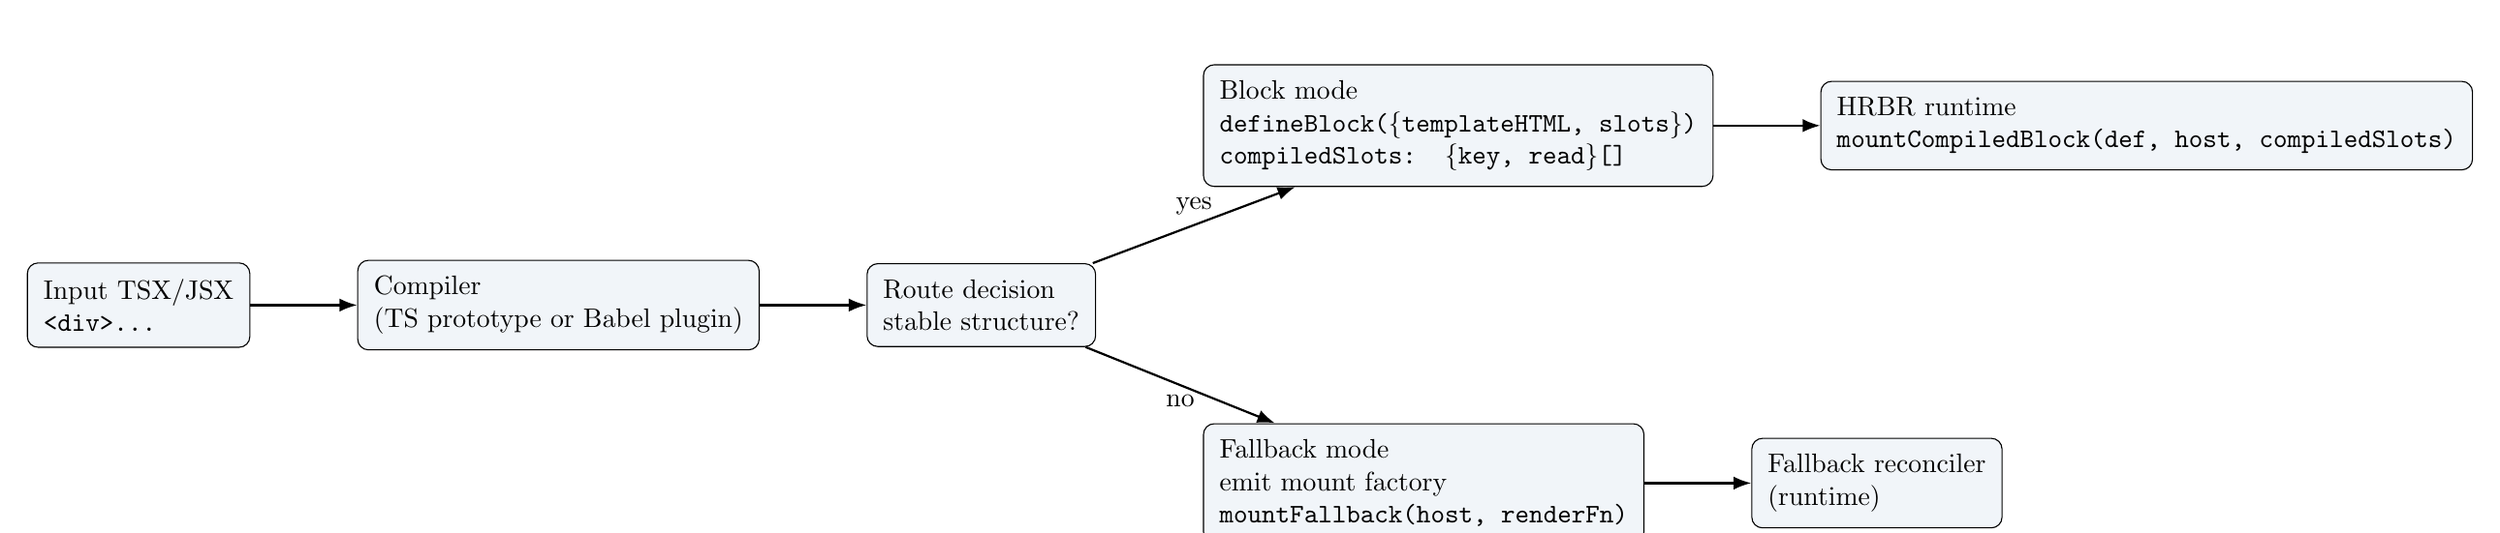
\begin{tikzpicture}[
	node distance=10mm and 14mm,
	box/.style={draw, rounded corners, align=left, inner sep=6pt, fill=RelaxLight},
	arrow/.style={-Latex, thick}
]
\node[box] (jsx) {Input TSX/JSX\\\texttt{<div>...}};
\node[box, right=of jsx] (compiler) {Compiler\\(TS prototype or Babel plugin)};
\node[box, right=of compiler] (decision) {Route decision\\stable structure?};

\node[box, above right=of decision] (block) {Block mode\\\texttt{defineBlock(\{templateHTML, slots\})}\\\texttt{compiledSlots: \{key, read\}[]}\;};
\node[box, below right=of decision] (fallback) {Fallback mode\\emit mount factory\\\texttt{mountFallback(host, renderFn)}};

\node[box, right=of block] (runtimeB) {HRBR runtime\\\texttt{mountCompiledBlock(def, host, compiledSlots)}};
\node[box, right=of fallback] (runtimeF) {Fallback reconciler\\(runtime)};

\draw[arrow] (jsx) -- (compiler);
\draw[arrow] (compiler) -- (decision);
\draw[arrow] (decision) -- node[midway, above] {yes} (block);
\draw[arrow] (decision) -- node[midway, below] {no} (fallback);
\draw[arrow] (block) -- (runtimeB);
\draw[arrow] (fallback) -- (runtimeF);
\end{tikzpicture}
\end{center}

This is the architectural backbone: the compiler emits either a \emph{BlockDef + read closures} (fast) or a \emph{fallback mount factory} (safe).

\subsection{Tiny contract (2 bullets)}

Given a JSX expression, the compiler must be able to produce one of:

\begin{itemize}
\item \textbf{Block mode (fast path):} \texttt{defineBlock({ templateHTML, slots })} plus a mount factory that calls \texttt{mountCompiledBlock(def, host, compiledSlots)}.
\item \textbf{Fallback mode (safe path):} a mount factory that calls \texttt{mountFallback(...)} and delegates structural reconciliation to the runtime.
\end{itemize}

The runtime intentionally does not know how compilation works; it only requires these shapes.

The HRBR runtime expects two main pieces of data.

\subsection{1) A \texttt{BlockDef}: stable template + slot metadata}

Defined in \texttt{runtime/block.ts}, a \texttt{BlockDef} contains:

\begin{itemize}
\item \texttt{templateHTML: string}, the stable HTML string that will be parsed once.
\item \texttt{slots: Record<string, BlockSlot>} , the mapping from a slot key to its write kind and a DOM path.
\end{itemize}

A \texttt{BlockSlot} describes \emph{what} to write (text/attr/class/style/prop/event, etc.) and \emph{where} to write it (a childNodes index path).

\subsection{2) A \texttt{CompiledSlot[]} list: how to read live values}

At runtime, \texttt{mountCompiledBlock(def, host, compiledSlots)} needs an array of objects shaped like:

\begin{quote}
\texttt{\{ key: string, read: () => unknown \}}
\end{quote}

The compiler can't always inline the read closures in a pure data file.
In particular, the TypeScript prototype compiler deliberately returns no reads; it records expression source code so a caller with lexical scope can build closures.

In contrast, the Babel transform \emph{can} emit \texttt{read: () => expr} arrow functions directly into the output program, precisely because it is already transforming a file with the correct lexical scope.

\subsection{A 3-part boundary you should memorize}

At the boundary, the compiler emits three things:

\begin{enumerate}
\item a \texttt{BlockDef} (pure data: stable HTML + slot metadata)
\item a \texttt{compiledSlots[]} list (closures: how to read live values)
\item a mount factory (a closure boundary: where lexical scope lives)
\end{enumerate}

That last bullet is easy to miss.
It\'s the reason the Babel transform can emit \texttt{read: () => expr} directly, while the TypeScript prototype compiler intentionally stops at ``expression source code''.

For a background overview of why JSX is typically compiled, see:\
\href{https://react.dev/learn/writing-markup-with-jsx}{https://react.dev/learn/writing-markup-with-jsx}.

\section{Routing decision: block vs fallback}

The compiler's core architectural decision is: \emph{can this TSX be represented as a stable HTML template?}
If not, we must use the fallback reconciler.

\subsection{Dynamic structure}

The term \textbf{dynamic structure} means ``the set/shape/order of DOM nodes can change as state changes.''
Examples:

\begin{itemize}
\item conditionals: \texttt{cond ? <div/> : null}
\item loops/lists: \texttt{items.map(...)}
\item fragments that change child count
\item dynamic tag names or component tags
\item spreading attributes (often implies unknown keys)
\item event handlers (in the current compiler phase) if they can't be represented as static bindings
\end{itemize}

Compiled blocks are designed for \emph{stable structure} with dynamic \emph{values}.
When structure is dynamic, we let the fallback runtime reconcile children.

\subsection*{Diagram: what counts as “dynamic structure” (conservative)}
\begin{center}
\begin{tikzpicture}[
	node distance=8mm and 12mm,
	box/.style={draw, rounded corners, align=left, inner sep=6pt, fill=RelaxLight},
	arrow/.style={-Latex, thick},
	decision/.style={draw, diamond, aspect=2, inner sep=2.5pt, align=center, fill=RelaxLight}
]
\node[box] (expr) {JSX expression\\\texttt{<div>...</div>}};
\node[decision, right=of expr] (dyn) {Any child\\expression can\\change node shape?};
\node[box, above right=of dyn] (fallback) {Route to fallback\\(reconcile structure)};
\node[box, below right=of dyn] (block) {Allow block mode\\(write values only)};

\draw[arrow] (expr) -- (dyn);
\draw[arrow] (dyn) -- node[midway, above] {yes} (fallback);
\draw[arrow] (dyn) -- node[midway, below] {no} (block);
\end{tikzpicture}
\end{center}

Relax’s current compilers deliberately err on the safe side: anything that could introduce or remove DOM nodes is treated as “dynamic structure”.

\subsection{A useful rule of thumb}

If an expression could evaluate to:

\begin{itemize}
\item \texttt{null}
\item \texttt{false}
\item an array of nodes
\item a \texttt{<div>} sometimes and \texttt{<span>} other times
\end{itemize}

then it’s structural and must go to fallback.

If it always evaluates to a \emph{value} that can be written into an existing node (text/attr/prop/class/style), then it can stay in block mode.

This is conservative, but it keeps the compiler honest.

\subsection{How ``block vs fallback'' relates to Chapter~\ref{ch:vdom-hrbr-interop}}

The compiler output doesn't mount directly into the VDOM. Instead, it produces a \emph{mount factory} that matches the HRBR vnode contract described in Chapter~\ref{ch:vdom-hrbr-interop}.
That is why the VDOM type \texttt{DOM\_TYPES.HRBR} stores a \texttt{mount(host)} function: it is the common denominator between compiled blocks and fallback regions.

\section{TypeScript prototype compiler (Phase 5 reference)}

The TypeScript implementation lives in \texttt{compiler/index.ts}.
It provides two public APIs:

\begin{itemize}
\item \texttt{compileTSXToBlock(source, opts?) -> CompileResult}
\item \texttt{compileTSXOrFallback(source, opts?) -> CompileOrFallbackResult}
\end{itemize}

\subsection{\texttt{compileTSXToBlock():} parse -> extract -> render template}

\textbf{Inputs}

\begin{itemize}
\item \texttt{source: string}: a single-root TSX expression (or a statement containing one).
\item \texttt{opts.fileName?}: helps TypeScript provide useful source locations.
\item \texttt{opts.strictTemplate?} (default true): reject patterns that can't be expressed as a static HTML template.
\end{itemize}

\textbf{Main pipeline}

\begin{enumerate}
\item Parse the input with TypeScript: \texttt{ts.createSourceFile(..., ScriptKind.TSX)}.
\item Find the first expression via \texttt{findFirstExpression()}.
\item Ensure the root is \texttt{JsxElement} or \texttt{JsxSelfClosingElement}.
\item Build a \texttt{TemplateBuild} using \texttt{buildTemplate()}.
\item Return \texttt{\{ block: \{templateHTML, slots\}, slots: [], meta \}}.
\end{enumerate}

\subsection{Determinism: why the TS compiler is a good executable spec}

The implementation in \texttt{compiler/index.ts} is deliberately small and deterministic:

\begin{itemize}
\item It parses with TypeScript's parser (so syntax + TSX rules match what users write).
\item It walks the syntax tree into a simple string renderer that produces \texttt{templateHTML}.
\item It computes slot paths using an explicit \texttt{childIndex} counter.
\end{itemize}

This makes it ideal for teaching and for pinning down invariants (especially path semantics) before committing to a more complex Babel visitor implementation.

\subsection{Paths: the compiler and runtime must agree}

The most important shared invariant between compiler and runtime is how a ``path'' is interpreted.

In this prototype compiler, each element maintains a \texttt{childIndex} counter, and each child node increments the counter as it is rendered.
When the compiler emits a slot, it records the current path (a list of child indices) that identifies a target node under the template root.

\paragraph{Why this works}

The block runtime later parses \texttt{templateHTML} into a DOM tree and walks \texttt{childNodes[index]} repeatedly to locate the slot target.

\subsection{The one gotcha that causes most bugs: \texttt{childNodes} includes text nodes}

If you take nothing else from this chapter, take this:

\begin{quote}
	extbf{Slot paths are based on DOM \texttt{childNodes}, not \texttt{children}.}
\end{quote}

That means whitespace and literal text in your template count as nodes.
So when you look at markup like:

\begin{quote}
	exttt{<p>Hello \{name()\}</p>}
\end{quote}

the compiled \texttt{templateHTML} might contain literal spaces or newlines, and those become \texttt{Text} nodes when parsed.

This is also why the tests talk about paths like \texttt{[3, 1]} (not \texttt{[0, 0]}).
In the Babel snapshot test (\texttt{compiler/\_\_tests\_\_/babel-transform.test.ts}), the template contains indentation and newlines.
When parsed, they become text nodes that affect indexing.

\subsection{Walkthrough: compute a slot path by hand}

Let\'s do a small thought experiment that matches the compiler\'s rules.

Input TSX:

\begin{lstlisting}[language=JavaScript]
const App = () => (
	<section id="root" className={cls()}>
		<h1>Title</h1>
		<p>Hello {name()}</p>
	</section>
)
\end{lstlisting}

The Babel transform snapshot illustrates this exact structure as a static template plus two slots:

\begin{itemize}
\item \texttt{s0}: a \texttt{class} slot on the root element, with \texttt{path: []}
\item \texttt{s1}: a \texttt{text} slot inside the \texttt{<p>}, with \texttt{path: [3, 1]}
\end{itemize}

Why \texttt{[3, 1]}?

\begin{itemize}
\item \texttt{[]} means \"start at the template root element\" (the \texttt{<section>}).
\item \texttt{3} means \"go to the 4th \texttt{childNodes} entry under \texttt{<section>}\".
	In formatted templates, the \texttt{childNodes} often look like: newline text, \texttt{<h1>}, newline text, \texttt{<p>}, newline text.
\item \texttt{1} then means \"go to the 2nd \texttt{childNodes} entry under \texttt{<p>}\".
		Under \texttt{<p>}, you often have: \texttt{Text('Hello ')} then \texttt{Text('\_\_hrbr\_\_')} (or an empty placeholder) depending on how the compiler encodes it.
\end{itemize}

This is ugly but reliable.
And reliability is the whole point: the compiler and runtime just need to agree.

For background on DOM node lists, see MDN:
\href{https://developer.mozilla.org/en-US/docs/Web/API/Node/childNodes}{https://developer.mozilla.org/en-US/docs/Web/API/Node/childNodes}.

\subsection{What the TS prototype actually returns (and why the reads are empty)}

In \texttt{compiler/index.ts}, \texttt{compileTSXToBlock()} returns:

\begin{itemize}
\item \texttt{block: \{ templateHTML, slots \}}
\item \texttt{slots: []} (yes, empty)
\item \texttt{meta} about dynamic structure, lanes, etc.
\end{itemize}

That\'s not a bug.
It\'s an explicit constraint: a string-only compiler doesn\'t have access to the lexical scope where \texttt{count()}, \texttt{cls()}, or \texttt{name()} live.
So it records the expression source code internally (\texttt{reads: \{key, code\}[]}) but does not pretend it can create closures.

The end-to-end test in \texttt{compiler/\_\_tests\_\_/compiler.e2e.test.ts} shows the intended integration:
the caller wires in the \texttt{read} closures manually.

\begin{lstlisting}[language=JavaScript]
const { block } = compileTSXToBlock(`(<div className={count()}>Count</div>)`)

const mounted = mountCompiledBlock(block, host, [
	{ key: 's0', read: () => count() },
])
\end{lstlisting}

The key behavioral contract in that test is worth repeating:

\begin{quote}
	extbf{Updating signals must never recreate the root element.}
\end{quote}

In other words, compilation is only useful if it reduces work to \emph{writes}, not \emph{mount/unmount}.

\section{Babel transform: how the output program is shaped}

The Babel plugin in \texttt{compiler/jsx/transform.ts} exists to solve the closure problem.
It runs inside your real source file, so it can emit \texttt{read: () => expr} in-place.

\subsection{The shape (as asserted by tests)}

The unit tests in \texttt{compiler/\_\_tests\_\_/babel-transform.test.ts} basically define the public contract.
The transform must emit:

\begin{itemize}
\item an import from \texttt{relax/hrbr} that includes \texttt{defineBlock} and \texttt{mountCompiledBlock}
\item a module-scope \texttt{const \_\_hrbr\_block\_N = defineBlock(...)}
\item component output that returns a \textbf{mount factory}: \texttt{host => \_\_hrbrBlock(host, def, slots)}
\item a wrapper function \texttt{\_\_hrbrBlock(host, def, slots)} that calls \texttt{mountCompiledBlock(def, host, slots)}
\end{itemize}

Here\'s the key part of the snapshot (reformatted as teaching code):

\begin{lstlisting}[language=JavaScript]
import { defineBlock, mountCompiledBlock } from "relax/hrbr";

const __hrbr_block_0 = defineBlock({
	templateHTML: "<section id=\"root\" class=\"\">\n...",
	slots: {
		"s0": { kind: "class", path: [] },
		"s1": { kind: "text", path: [3, 1] },
	}
});

const App = () => host => __hrbrBlock(host, __hrbr_block_0, [
	{ key: "s0", read: () => cls() },
	{ key: "s1", read: () => name() },
]);

function __hrbrBlock(host, def, slots) {
	return mountCompiledBlock(def, host, slots);
}
\end{lstlisting}

There are two deeply important design choices here:

\begin{enumerate}
\item \textbf{The \texttt{BlockDef} is module-scope data.}
	It should be created once, not per render.
\item \textbf{The mount factory is per render, and it closes over reads.}
	That\'s where \texttt{cls()} and \texttt{name()} are actually in scope.
\end{enumerate}

This pattern is very similar in spirit to Solid\'s compilation strategy (static DOM + fine-grained updates), though the runtime and APIs differ.
For a conceptual reference, see:
\href{https://www.solidjs.com/docs/latest\#compiling}{https://www.solidjs.com/docs/latest\#compiling}.

\subsection{Lane pragmas: compiler-to-scheduler hints without changing semantics}

Both compilers support a tiny \"lane pragma\" syntax:

\begin{lstlisting}[language=JavaScript]
<div
	className={/*@lane transition*/ cls()}
	data-x={/*@lane input*/ x()}
/>
\end{lstlisting}

The Babel test asserts that these land in slot metadata as \texttt{lane: "transition"} and \texttt{lane: "input"}.

Why it matters: when you start integrating compilation into an app/runtime scheduler, this gives you a way to nudge \emph{when} updates flush without changing \emph{what} updates mean.

\section{Debugging: when a slot path is wrong}

The most common failure mode when you build a compiler like this is:\
	extbf{the slot writes go to the wrong node.}

When that happens, you should immediately suspect one of these:

\begin{itemize}
\item you counted \texttt{children} instead of \texttt{childNodes}
\item your template string gained or lost whitespace (newlines/indentation)
\item you treated a void tag as having children (or forgot it closes itself)
\end{itemize}

\subsection*{Mini-exercise (tests-as-spec)}

Open \texttt{compiler/\_\_tests\_\_/babel-transform.test.ts} and find the inline snapshot where \texttt{path: [3, 1]}.
Then:

\begin{enumerate}
\item remove the whitespace/newlines in the template emitter (so the HTML becomes a single line),
\item update the snapshot, and
\item explain (in one sentence) why the path changed.
\end{enumerate}

This is the simplest way to internalize the \texttt{childNodes} rule.

The critical detail is that the compiler counts \emph{every child node} (elements \emph{and} text nodes), because \texttt{childNodes} includes text nodes. In \texttt{compiler/index.ts} this is represented by \texttt{PathState\{ childIndex \}}.

This is also why the compiler uses explicit sentinels for some dynamic expressions: it needs to ensure a real, countable node exists at the path.

\subsection*{Diagram: how slot paths are interpreted via \texttt{childNodes}}
\begin{center}
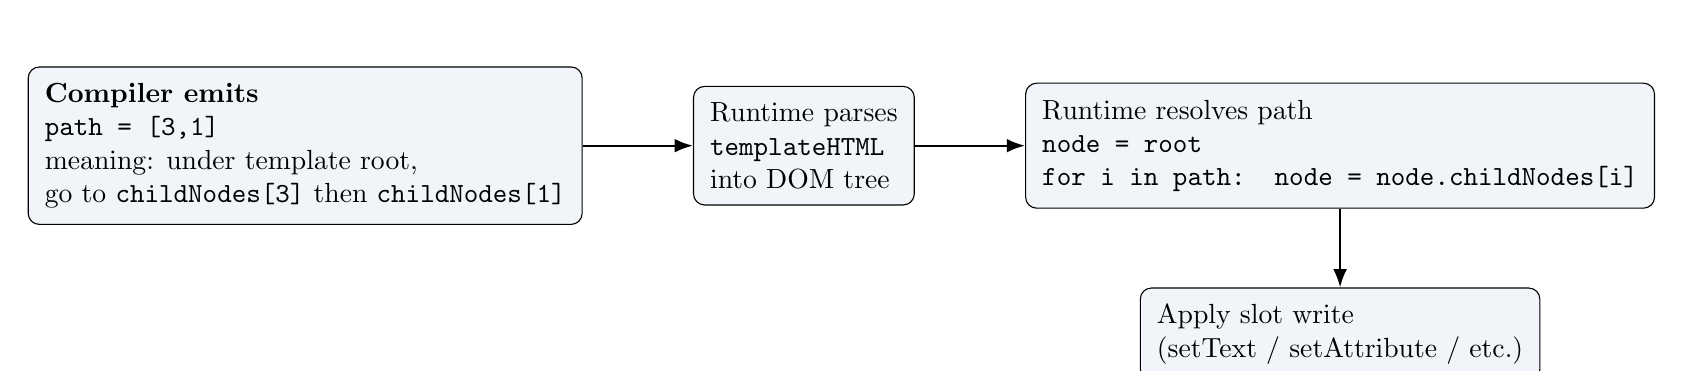
\begin{tikzpicture}[
	node distance=10mm and 14mm,
	box/.style={draw, rounded corners, align=left, inner sep=6pt, fill=RelaxLight},
	arrow/.style={-Latex, thick}
]
\node[box] (template) {\textbf{Compiler emits}\\\texttt{path = [3,1]}\\meaning: under template root,\\go to \texttt{childNodes[3]} then \texttt{childNodes[1]}};
\node[box, right=of template] (parse) {Runtime parses\\\texttt{templateHTML}\\into DOM tree};
\node[box, right=of parse] (walk) {Runtime resolves path\\\texttt{node = root}\\\texttt{for i in path: node = node.childNodes[i]}};
\node[box, below=of walk] (write) {Apply slot write\\(setText / setAttribute / etc.)};

\draw[arrow] (template) -- (parse);
\draw[arrow] (parse) -- (walk);
\draw[arrow] (walk) -- (write);
\end{tikzpicture}
\end{center}

This is why both compilers count \emph{text nodes} as children: the runtime uses \texttt{childNodes}, not \texttt{children}.

\subsection{Text expression handling: sentinel + slot path}

In \texttt{renderJSX()}, when a child is \texttt{JsxExpression}:

\begin{itemize}
\item the compiler marks \texttt{meta.hasDynamicStructure = true}
\item it allocates a slot key \texttt{sN}
\item it emits a unique sentinel string \texttt{\_\_hrbr\_sN\_\_} into the template
\item it records a \texttt{text} slot whose path points to that text node
\item it records the expression's source text as a ``read'' entry
\end{itemize}

This is a deliberately conservative design: any child expression could be a conditional or a list, so the prototype treats it as structure-changing.
The Babel compiler (later in this book) uses heuristics to allow some expressions as ``text-like'' without falling back.

\subsection{Void elements and template correctness}

The TS compiler treats HTML void tags specially via the \texttt{VOID\_TAGS} set.
For these tags it emits \texttt{<input ...>} rather than \texttt{<input ...></input>}.
This matters because the runtime parses \texttt{templateHTML} through \texttt{<template>} and relies on the browser's HTML parser to build a stable node tree. Producing non-HTML-canonical markup can shift the parsed tree and break slot paths.

\subsection{Attributes: literals vs expression slots}

The prototype supports:

\begin{itemize}
\item boolean attributes: \texttt{<div hidden />}
\item string literal attributes: \texttt{<div id="x" />}
\item expression attributes: \texttt{<div className=\{count()\} />}
\end{itemize}

Expression attributes allocate slot keys and record \texttt{kind} and \texttt{name}:

\begin{itemize}
\item \texttt{className} normalizes to \texttt{class}
\item \texttt{style} maps to a \texttt{style} slot
\item anything else becomes an \texttt{attr} slot
\end{itemize}

The compiler also records lane hints (per slot) and ``signal-like'' hints:

\begin{itemize}
\item \texttt{meta.lanesByKey}: a compiler-to-runtime hint used by schedulers in later phases
\item \texttt{meta.signalLikeByKey}: a heuristic that recognizes \texttt{foo()} style getters
\end{itemize}

Even when later phases choose to ignore (or reinterpret) these hints, keeping the meta separate from the structural template makes it possible to evolve scheduling policy without changing the fundamental block ABI.

\subsection{Fallback decision wrapper: \texttt{compileTSXOrFallback()}}

This wrapper is the ``policy layer'' on top of template extraction.
It answers one question: \emph{is it safe to run in block mode?}

At the top level, the TS prototype exposes a convenience API:
	exttt{compileTSXOrFallback(source)}.

Its semantics are intentionally boring:

\begin{lstlisting}[language=JavaScript]
const res = compileTSXToBlock(source)

if (res.meta.hasDynamicStructure) {
	return { kind: 'fallback', reason: 'dynamic-structure', meta: res.meta }
}

return { kind: 'block', ...res }
\end{lstlisting}

This is important because it makes ``fallback'' a first-class output, not an exception.
The compiler is allowed to say ``I don't know''.

\section{Dynamic structure detection (what triggers fallback)}

Now we'll make the fuzzy idea from earlier (\emph{structure vs values}) precise.
The easiest way is to turn the implementation into a checklist.

\subsection{Decision table: TS prototype vs Babel transform}

Relax currently has a \emph{conservative} detector in the TS prototype and a \emph{slightly more permissive} detector in the Babel transform.
They differ because Babel has access to more information (and can safely reject with fallback by returning \texttt{null} from template building).

\begin{center}
\begin{tabular}{|p{0.34\textwidth}|p{0.29\textwidth}|p{0.29\textwidth}|}
\hline
	extbf{Input pattern} & \textbf{TS prototype (\texttt{compiler/index.ts})} & \textbf{Babel transform (\texttt{compiler/jsx/transform.ts})}\\
\hline
Child expression: \texttt{<p>Hello \{expr\}</p>} & Marks \texttt{meta.hasDynamicStructure = true} (always) & Allows only \emph{text-like} expressions; otherwise returns \texttt{null} to route to fallback \\
\hline
Conditional/logical children: \texttt{cond ? <A/> : <B/>}, \texttt{cond \&\& <A/>} & Treated as dynamic structure (child expression) & Treated as ``not text-like'' (\texttt{ConditionalExpression}/\texttt{LogicalExpression}); routes to fallback \\
\hline
Non-intrinsic tags: \texttt{<Component/>}, \texttt{<Foo.Bar/>} & Marks dynamic structure when tag is not lowercase & Template builder returns \texttt{null} when tag is not a lowercase intrinsic \\
\hline
Event handlers: \texttt{onClick=\{fn\}} & Marks dynamic structure (events not representable in static HTML) & Immediately returns \texttt{null} (block mode not supported for events yet) \\
\hline
Spread attributes: \texttt{<div \{...props\} />} & Marks dynamic structure (and throws in strict template mode) & Returns \texttt{null} (not supported in block template) \\
\hline
Void tags: \texttt{<input/>}, \texttt{<img/>} & Emitted with correct HTML void syntax via \texttt{VOID\_TAGS} & Emitted with a regex-based void-tag check \\
\hline
\end{tabular}
\end{center}

This table is the practical meaning of \emph{``dynamic structure''} in Relax today.

\subsection{Babel's \texttt{isTextLikeExpr}: the tiny heuristic that buys you a lot}

The Babel transform has a helper called \texttt{isTextLikeExpr(expr)}.
The idea is simple: if a child expression could evaluate to an element/fragment/array, then the template structure isn't stable.
But if it's always a value that can be written into \texttt{textContent}, we can keep block mode.

From the scaffold (summarized):

\begin{lstlisting}[language=JavaScript]
function isTextLikeExpr(expr) {
	if (expr is JSXElement or JSXFragment) return false
	if (expr is ConditionalExpression) return false
	if (expr is LogicalExpression) return false
	return true
}
\end{lstlisting}

Notice what this buys us:

\begin{itemize}
\item \textbf{Text updates stay cheap.} Most UIs do a lot of ``render some string'' work.
\item \textbf{You can still escape hatch.} The moment an expression might be structural, it falls back.
\end{itemize}

This is a deliberately small heuristic.
In later chapters, you'll see how it grows, and how tests keep it honest.

\section{Babel compilation mechanics: how one JSX element becomes a block}

So far we've looked at the \emph{shape} of the output.
Now we'll build a mental model for the \emph{mechanics} of how the Babel transform creates that output.

The transform in \texttt{compiler/jsx/transform.ts} does three jobs:

\begin{enumerate}
\item build a static HTML template string
\item allocate slots + paths for the dynamic parts
\item emit a mount factory that closes over live reads
\end{enumerate}

If you understand those three, the whole transform stops feeling magical.

\subsection{Step 1: pick a stable root (or give up)}

The transform only wants to compile stable, intrinsic HTML tags like \texttt{div}, \texttt{section}, and \texttt{button}.
If the tag is not a lowercase intrinsic (for example \texttt{<Component/>} or \texttt{<Foo.Bar/>}), there is no obvious static HTML representation.
So the template builder returns \texttt{null}, and the plugin routes to fallback.

Why is this the right default?

\begin{itemize}
\item In JSX, a capitalized tag means ``call some function and let it return anything''.
\item That means the compiler can't promise stable structure.
\end{itemize}

Block mode only works when the compiler can promise that \emph{the same DOM nodes exist forever}.

\subsection{Step 2: render a string that the browser will parse deterministically}

Think of compilation as emitting a \texttt{<template>} string.
Your compiler isn't building DOM; the browser will.
So your job is just to produce a string that will be parsed into a stable tree.

That implies two constraints:

\begin{itemize}
\item \textbf{Void tags matter.} \texttt{<input>} can't accidentally become \texttt{<input></input>}.
\item \textbf{Whitespace matters.} Newlines/indentation become text nodes and shift \texttt{childNodes} indices.
\end{itemize}

This is why the snapshot tests in \texttt{compiler/\_\_tests\_\_/babel-transform.test.ts} are so valuable.
They lock down not just the slot paths, but the \emph{exact} template string (including newlines).

\subsection{Step 3: allocate slots: ``static HTML with holes''}

When the transform sees something dynamic, it does \emph{not} generate DOM operations directly.
It just records metadata that the runtime knows how to apply later.

You can think of slot allocation as making a table that answers:

\begin{quote}
When the runtime mounts this template, \emph{where} is the thing to update, and \emph{how} should it be updated?
\end{quote}

Examples you should expect as you read the code:

\begin{itemize}
\item \textbf{Attribute slot:} dynamic attribute value (\texttt{kind: 'attr'}).
\item \textbf{Class slot:} \texttt{className=\{...\}} normalized to \texttt{class} (\texttt{kind: 'class'}).
\item \textbf{Text slot:} dynamic text content inside an element (\texttt{kind: 'text'}).
\end{itemize}

Every slot includes a \texttt{path}, which is just a frozen version of the \texttt{childNodes} walk we discussed earlier.

\subsection{Step 4: emit reads as closures (the key Babel advantage)}

The TS prototype can't produce \texttt{read: () => expr} because it doesn't know which variables exist.
But Babel is transforming your actual file, so it can emit closures that reference \texttt{cls()}, \texttt{name()}, or any local binding.

The key idea is:

\begin{quote}
	extbf{All dynamic values are read through closures passed to \texttt{mountCompiledBlock()}.}
\end{quote}

This means compilation doesn't change your state model.
Signals are still signals.
The compiler just gives the runtime a faster way to apply their values.

\subsection{Step 5: fallback routing is just ``emit a different mount factory''}

In the Babel plugin, ``fallback'' isn't a special runtime mode.
It's just a different function call in the generated output:

\begin{itemize}
\item block mode: emit \texttt{mountCompiledBlock(def, host, compiledSlots)}
\item fallback mode: emit \texttt{mountFallback(host, () => <JSX...>)} (shape varies as the scaffold evolves)
\end{itemize}

The important part is the architecture: both modes still return a mount function.
So the caller doesn't care which one it got.

For conceptual background on why many UI frameworks separate ``render'' from ``commit'' (build a description then apply it), see:
\href{https://react.dev/learn/render-and-commit}{https://react.dev/learn/render-and-commit}.

\section{Validation contract: how to change the compiler safely}

Compilers are notoriously easy to break with tiny edits.
Relax deals with this by treating tests as the spec.
If you're modifying the compiler, keep these two mental buckets:

\begin{itemize}
\item \textbf{Behavioral contracts:} integration tests that assert DOM stability.
\item \textbf{Shape contracts:} snapshot tests that assert exact emitted output.
\end{itemize}

\subsection{Spec-to-test mapping (start here when debugging)}

\begin{itemize}
\item \textbf{"Don't recreate root DOM" contract:} \texttt{compiler/\_\_tests\_\_/compiler.e2e.test.ts}
\item \textbf{"Exact codegen shape" contract (imports, defineBlock, wrapper):} \texttt{compiler/\_\_tests\_\_/babel-transform.test.ts}
\item \textbf{"Path semantics" contract (whitespace affects \texttt{childNodes}):} also \texttt{babel-transform.test.ts} snapshots
\end{itemize}

When you're unsure whether a change is safe, prefer adding a tiny unit test over adding another heuristic.
Heuristics get clever; tests keep you honest.

Now we\'ll make the fuzzy idea from earlier (\emph{structure vs values}) precise.
The easiest way is to turn the implementation into a checklist.

\subsection{Decision table: TS prototype vs Babel transform}

Relax currently has a \emph{conservative} detector in the TS prototype and a \emph{slightly more permissive} detector in the Babel transform.
They differ because Babel has access to more information (and can safely reject with fallback by returning \texttt{null} from template building).

\begin{center}
\begin{tabular}{|p{0.34\textwidth}|p{0.29\textwidth}|p{0.29\textwidth}|}
\hline
	extbf{Input pattern} & \textbf{TS prototype (\texttt{compiler/index.ts})} & \textbf{Babel transform (\texttt{compiler/jsx/transform.ts})}\\
\hline
Child expression: \texttt{<p>Hello \{expr\}</p>} & Marks \texttt{meta.hasDynamicStructure = true} (always) & Allows only \emph{text-like} expressions; otherwise returns \texttt{null} to route to fallback \\
\hline
Conditional/logical children: \texttt{cond ? <A/> : <B/>}, \texttt{cond \&\& <A/>} & Treated as dynamic structure (child expression) & Treated as \\"not text-like\\" (\texttt{ConditionalExpression}/\texttt{LogicalExpression}); routes to fallback \\
\hline
Non-intrinsic tags: \texttt{<Component/>}, \texttt{<Foo.Bar/>} & Marks dynamic structure when tag is not lowercase & Template builder returns \texttt{null} when tag is not a lowercase intrinsic \\
\hline
Event handlers: \texttt{onClick=\{fn\}} & Marks dynamic structure (events not representable in static HTML) & Immediately returns \texttt{null} (block mode not supported for events yet) \\
\hline
Spread attributes: \texttt{<div \{...props\} />} & Marks dynamic structure (and throws in strict template mode) & Returns \texttt{null} (not supported in block template) \\
\hline
Void tags: \texttt{<input/>}, \texttt{<img/>} & Emitted with correct HTML void syntax via \texttt{VOID\_TAGS} & Emitted with a regex-based void-tag check \\
\hline
\end{tabular}
\end{center}

This table is the practical meaning of \emph{\"dynamic structure\"} in Relax today.

\subsection{Babel\'s \texttt{isTextLikeExpr}: the tiny heuristic that buys you a lot}

The Babel transform has a helper called \texttt{isTextLikeExpr(expr)}.
The idea is simple: if a child expression could evaluate to an element/fragment/array, then the template structure isn\'t stable.
But if it\'s always a value that can be written into \texttt{textContent}, we can keep block mode.

From the scaffold (summarized):

\begin{lstlisting}[language=JavaScript]
function isTextLikeExpr(expr) {
	if (expr is JSXElement or JSXFragment) return false
	if (expr is ConditionalExpression) return false
	if (expr is LogicalExpression) return false
	return true
}
\end{lstlisting}

Notice what this buys us:

\begin{itemize}
\item \texttt{<span>{count()}</span>} can be compiled as a text slot.
\item \texttt{<span>{count() > 0 ? <b/> : null}</span>} must go to fallback.
\end{itemize}

Even though this is conservative, it gets you most of the performance wins for the common case (text/attr/class/style bindings).

\section{How fallback routing looks in the Babel output (scaffold)}

When \texttt{buildTemplateFromJsxElement()} returns \texttt{null}, the plugin constructs a minimal \texttt{mountFallback()} call.
This is still early-stage code, but it\'s worth understanding the design:

\begin{itemize}
\item block mode emits a \texttt{BlockDef} and a tight \texttt{CompiledSlot[]} list
\item fallback emits a \emph{render function} that returns reconciliation specs (create/patch)
\end{itemize}

That means fallback is not \"VDOM\" in the React sense.
It\'s a small structural reconciler that still aims to avoid recreating nodes whenever possible.

If you want a conceptual baseline for why compilers do this \"static template + runtime writes\" split, React\'s docs on render/commit are a good mental model:
\href{https://react.dev/learn/render-and-commit}{https://react.dev/learn/render-and-commit}.

\subsection*{Spec-to-test mapping (what to read next)}

When you\'re debugging compiler behavior, treat these tests as your spec:

\begin{itemize}
\item \textbf{No DOM recreation on updates}: \texttt{compiler/\_\_tests\_\_/compiler.e2e.test.ts}
\item \textbf{Output program shape}: \texttt{compiler/\_\_tests\_\_/babel-transform.test.ts}
\end{itemize}

If a behavior isn't asserted there yet, it's not stable.

\texttt{compileTSXOrFallback()} runs \texttt{compileTSXToBlock()} and then returns:

\begin{itemize}
\item \texttt{\{ kind: 'fallback', reason: 'dynamic-structure' \}} if \texttt{meta.hasDynamicStructure} is true
\item otherwise \texttt{\{ kind: 'block', ...result \}}
\end{itemize}

This is the high-level policy the real Babel transform is evolving toward.

Note the important nuance: \texttt{compileTSXToBlock()} still returns a \texttt{BlockDef} even when \texttt{meta.hasDynamicStructure} is true. That mirrors how the Babel plugin can still hoist block defs for other expressions in the same file even if one subtree needs fallback.

\section{Babel transform scaffold (real-world integration)}

The Babel plugin entrypoint is exported as \texttt{hrbrJsxTransform} from \texttt{compiler/jsx/index.ts} and re-exported from \texttt{compiler/index.ts}.
The implementation lives in \texttt{compiler/jsx/transform.ts}.

\subsection{Roles of the Babel plugin}

Compared to the TS prototype, the Babel plugin has additional responsibilities:

\begin{itemize}
\item Operate on full program files, not just an isolated expression string.
\item Inject runtime imports: \texttt{defineBlock}, \texttt{mountCompiledBlock}, and optionally \texttt{mountFallback}.
\item Generate wrapper helpers (e.g. \texttt{\_\_hrbrBlock}) that connect emitted data literals to runtime calls.
\item Derive stable slot keys in dev mode (optionally) so diffs are readable.
\end{itemize}

\subsection{``Block mode'' is best-effort: return \texttt{null} to fall back}

The internal function \texttt{buildTemplateFromJsxElement()} tries to convert a JSX element into:

\begin{itemize}
\item \texttt{templateHTML}
\item \texttt{slots} map
\item \texttt{compiledSlots} array literal (with \texttt{read: () => expr})
\end{itemize}

If it sees unsupported patterns (events, dynamic elements, structural expressions), it returns \texttt{null} and marks that fallback imports are needed.

\subsection{Babel transform: what ``best-effort block mode'' means in code}

In \texttt{compiler/jsx/transform.ts}, block mode is essentially:

\begin{itemize}
\item Try to turn a \texttt{JSXElement} into \texttt{\{ templateHTML, slots, compiledSlots \}} using \texttt{buildTemplateFromJsxElement()}.
\item If any unsupported structure appears, return \texttt{null}.
\item The caller then chooses a fallback mount factory instead of a compiled-block mount factory.
\end{itemize}

The current transform is strict on purpose (e.g. it rejects events and spreads in block mode), because the project is trying to keep the block subset crisp while the fallback runtime is still evolving.

\subsection{Slot key strategies: sequential vs stable (dev mode)}

The Babel compiler contains two different slot key allocation styles:

\begin{itemize}
\item \textbf{Default (prod-like):} sequential keys \texttt{s0, s1, ...}.
\item \textbf{Dev mode:} location-based keys like \texttt{s\_text\_12:18} derived from source positions.
\end{itemize}

Location-based keys are helpful because they reduce ``slot churn'' in diffs and make debugging invalid-path errors more readable.

\subsection{Lane pragmas (compiler-to-scheduler hint)}

The Babel plugin recognizes comment pragmas in expression containers:

\begin{quote}
\texttt{className=\{/*@lane transition*/ cls()\}}
\end{quote}

It extracts the lane and stores it on the slot metadata.
Later chapters will connect this to the deterministic scheduler.

Concretely, \texttt{extractLanePragmaFromExpressionContainer()} scans leading comments for a pattern like:\\
	texttt{@lane transition}.
When found, the compiler attaches \texttt{lane: "transition"} to the slot metadata object.

\section{Tests-as-spec}

The compiler has three layers of tests:

\begin{itemize}
\item Unit compilation tests (shape of emitted template/slots): \texttt{compiler/\_\_tests\_\_/compiler.test.ts}
\item Snapshot tests for stability: \texttt{compiler/\_\_tests\_\_/compiler.snapshot.test.ts}
\item End-to-end tests that mount the result in jsdom:
  \begin{itemize}
  \item \texttt{compiler/\_\_tests\_\_/compiler.e2e.test.ts} (TS prototype -> mountCompiledBlock)
  \item \texttt{compiler/\_\_tests\_\_/babel-transform.e2e-jsdom.test.ts} (Babel output -> evaluate -> mountCompiledBlock)
  \end{itemize}
\end{itemize}

In the rest of this section, we'll treat the tests as a specification of the compiler/runtime boundary.
We won't run them here, but reading them tells you what changes are allowed without breaking the public contract.

\subsection{Unit tests (TS): compile + mount sanity}


	extbf{File:} \texttt{compiler/\_\_tests\_\_/compiler.test.ts}

This test anchors the smallest happy path:

\begin{itemize}
\item \texttt{compileTSXToBlock()} accepts a simple intrinsic element with a dynamic attribute expression.
\item The caller supplies \texttt{CompiledSlot\{ key: 's0', read: () => name() \}}.
\item \texttt{mountCompiledBlock()} produces DOM matching the template, and the dynamic slot lands in the right place.
\end{itemize}

One subtle detail: the test disposes the mounted block via \texttt{mounted.dispose()}. This keeps the contract clear: compiled mounts are still reactive, and disposal is part of the lifecycle.

\subsection{TS end-to-end: compile -> mount -> update without recreating root}

In \texttt{compiler/\_\_tests\_\_/compiler.e2e.test.ts}:

\begin{enumerate}
\item Create a signal: \texttt{const [count, setCount] = createSignal(1)}.
\item Compile TSX: \texttt{(<div className=\{count()\}>Count</div>)}.
\item Mount via \texttt{mountCompiledBlock(block, host, \{ key: 's0', read: () => count() \})}.
\item Update the signal, wait for the scheduler (microtask + \texttt{setTimeout(0)}).
\item Assert the root element identity is preserved and only the class changed.
\end{enumerate}

This is the key end-to-end contract for compiled blocks.

This test also documents a scheduling assumption: it comments that HRBR scheduling uses \texttt{setTimeout(0)} by default in tests, so updates require waiting at least one timer tick.

\subsection{Babel transform unit tests: shape of emitted program}


	extbf{File:} \texttt{compiler/\_\_tests\_\_/babel-transform.test.ts}

These tests assert that the plugin is producing the intended \emph{program shape}:

\begin{itemize}
\item it injects an import from the configured runtime path (default \texttt{relax/hrbr})
\item it references \texttt{defineBlock} and \texttt{mountCompiledBlock}
\item it hoists a \texttt{const \_\_hrbr\_block\_0 = defineBlock(...)}
\item it emits a wrapper mount function of the form \texttt{host => \_\_hrbrBlock(host, def, slots)}
\end{itemize}

The snapshot test in this file is especially important: it pins down the exact emitted structure (templateHTML string, slots map, and compiledSlots array with \texttt{read: () => expr}).

The suite also asserts two ``developer experience'' guarantees:

\begin{itemize}
\item lane pragmas are propagated to slot metadata
\item dev mode can emit location-based keys
\end{itemize}

\subsection{Babel transform errors: the intentional block-mode subset}


	extbf{File:} \texttt{compiler/\_\_tests\_\_/babel-transform.errors.test.ts}

This suite documents what is currently \emph{rejected} in block mode:

\begin{itemize}
\item event handlers (e.g. \texttt{onClick})
\item spread attributes (\texttt{<div \{...props\} />})
\item fragments (\texttt{<>...</>})
\item non-intrinsic tags (components like \texttt{<Foo />})
\end{itemize}

Even if future versions route these to fallback instead of throwing, the existence of these tests is useful: it makes the current compilation subset explicit and prevents accidental expansion that would silently generate incorrect templates.

\subsection{Babel transform E2E (jsdom): evaluate emitted literals + mount}


	extbf{File:} \texttt{compiler/\_\_tests\_\_/babel-transform.e2e-jsdom.test.ts}

This test checks something subtle but crucial: the compiler output is not just syntactically valid---its emitted \emph{data} can actually be evaluated and mounted.

Notable aspects:

\begin{itemize}
\item It extracts the object literal passed to \texttt{defineBlock(...)} from the emitted text.
\item It extracts the compiledSlots array literal from the wrapper call.
\item It evaluates those two pieces with \texttt{new Function(...)} while providing \texttt{cls()} and \texttt{name()} from the test scope.
\item It mounts using \texttt{mountCompiledBlock} and asserts identity preservation across updates.
\end{itemize}

This approximates how ``real code'' will behave: the compile-time output must work with runtime scope (signals) and produce stable DOM.

\section{Worked example: derive \texttt{templateHTML} and slot paths from the snapshot}

Now we\'ll do the most valuable \emph{derive-it-by-hand} exercise: take the golden snapshot in
	exttt{compiler/\_\_tests\_\_/babel-transform.test.ts} and derive the template and slot paths by hand.
If you can do this once, debugging a compiler becomes much less mysterious.

\subsection{The input JSX (what the author writes)}

The snapshot test compiles this input:

\begin{lstlisting}[language=JavaScript]
const App = () => (
	<section id="root" className={cls()}>
		<h1>Title</h1>
		<p>Hello {name()}</p>
	</section>
)
\end{lstlisting}

At a high level, the compiler must split this into:

\begin{itemize}
\item \textbf{Structure:} a static HTML template string.
\item \textbf{Values:} a list of dynamic slots with deterministic DOM paths.
\end{itemize}

\subsection{Step 1: the static template string (structure + placeholders)}

In the normalized snapshot, the transform emits a \texttt{defineBlock({ templateHTML, slots })} where \texttt{templateHTML} is a single string.
It contains the \texttt{<section>} with \texttt{id="root"}, plus an empty \texttt{class=""} placeholder.

In the snapshot, the template also includes indentation and newlines.
That\'s not just cosmetic: when the runtime parses HTML, whitespace becomes text nodes.

Why the placeholders matter:

\begin{itemize}
\item \texttt{className=\{cls()\}} becomes \texttt{class=""} in the template so the runtime can later write the real attribute value.
\item \texttt{Hello \{name()\}} becomes \texttt{Hello  } in the template (leaving a stable ``spot'' for the text slot).
\end{itemize}

If you ever see a compiler try to ``just concatenate strings'' at runtime, this is the key difference: HRBR wants the template to be parsed once, and then updated via direct DOM writes.

\subsection{Step 2: the slot declarations (what to write + where to write it)}

The same snapshot asserts two slot declarations:

\begin{itemize}
\item \texttt{s0}: \texttt{kind: "class"}, \texttt{path: []}
\item \texttt{s1}: \texttt{kind: "text"}, \texttt{path: [3, 1]}
\end{itemize}

Think of \texttt{path} as a precomputed set of array indexes into \texttt{childNodes}.
No search. No diff. Just indexing.

\subsection{Step 3: compute \texttt{path: [3, 1]} by hand (the whitespace trap)}

We\'ll compute \texttt{[3, 1]} mechanically.

First hop: \texttt{3} means we\'re selecting \texttt{section.childNodes[3]}.
Because the template contains whitespace between elements, the \texttt{childNodes} list includes \emph{text nodes}:

\begin{enumerate}
\item \texttt{childNodes[0]}: text (newline/indent before \texttt{<h1>})
\item \texttt{childNodes[1]}: \texttt{<h1>}
\item \texttt{childNodes[2]}: text (newline/indent between \texttt{</h1>} and \texttt{<p>})
\item \texttt{childNodes[3]}: \texttt{<p>}
\item \texttt{childNodes[4]}: text (newline/indent before \texttt{</section>})
\end{enumerate}

So hop 1 lands on the \texttt{<p>}.

Second hop: \texttt{1} means \texttt{p.childNodes[1]}.
The \texttt{<p>} contains static text (\texttt{Hello }) plus a dynamic text slot.
The compiler\'s job is to ensure there\'s a stable text node representing the dynamic value.
So we get:

\begin{itemize}
\item \texttt{p.childNodes[0]}: text node for \texttt{"Hello "}
\item \texttt{p.childNodes[1]}: text node that will receive \texttt{name()} updates
\end{itemize}

That\'s what \texttt{path: [3, 1]} means: ``the second text node inside the paragraph.''

This is the most important compiler invariant in HRBR: if you change the template emitter and accidentally add/remove whitespace, you can shift every downstream path.

\subsection{Step 4: compiled slot readers (how values cross the boundary)}

The final piece the snapshot asserts is the compiled slot array literal:

\begin{lstlisting}[language=JavaScript]
const App = () => host => __hrbrBlock(host, __hrbr_block_0, [
	{ key: "s0", read: () => cls() },
	{ key: "s1", read: () => name() },
])
\end{lstlisting}

This is where Babel shines: \texttt{read} is a closure in the output program.
There\'s no serialization format for expressions.
The emitted code just calls the original functions.

\subsection{Debugging checklist (tests-first)}

When a compiled block updates the wrong node, treat it like a deterministic math error.
Use the tests to narrow it down:

\begin{enumerate}
\item Check the snapshot: \texttt{compiler/\_\_tests\_\_/babel-transform.test.ts}.
  If your change modified whitespace in \texttt{templateHTML}, you probably shifted paths.
\item Recompute the \texttt{childNodes} list by hand and see if the asserted \texttt{path} still lands on the intended node.
\item Run the E2E that actually mounts the evaluated literals:
  	exttt{compiler/\_\_tests\_\_/babel-transform.e2e-jsdom.test.ts}.
\end{enumerate}

If you get into the habit of adding a snapshot test first, you\'ll catch most path regressions before they reach runtime.

\subsection{Babel fallback E2E (jsdom): structural expression routes to \texttt{mountFallback}}


	extbf{File:} \texttt{compiler/\_\_tests\_\_/babel-transform.fallback.e2e-jsdom.test.ts}

This suite pins down the fallback routing policy:

\begin{itemize}
\item A conditional expression in children is treated as \textbf{dynamic structure} (unsafe for block mode).
\item The transform output must include \texttt{mountFallback}.
\item The emitted module is evaluated, and calling \texttt{App()} returns a mount function.
\item Updates are reactive: signal changes trigger DOM updates without throwing.
\end{itemize}

The test includes a comment that the MVP fallback spec doesn't yet clear conditional text in all cases; the contract being asserted is deliberately smaller: the pipeline compiles, mounts, and updates safely.

\section{Where we go next}

Chapter~\ref{ch:babel-plugin} will zoom in on the Babel visitor model and show how the plugin emits the full final shape that user code will run.
We will also connect the ``fail block mode'' paths to the fallback runtime and reconciler described earlier.

\section{Online resources}

\begin{itemize}
\item TypeScript compiler API: parsing source and working with AST nodes:\\
\href{https://github.com/microsoft/TypeScript/wiki/Using-the-Compiler-API}{TypeScript Wiki: Using the Compiler API}.

\item Babel plugin authoring and visitor model:\\
\href{https://babeljs.io/docs/en/plugins}{Babel docs: plugins},\\
\href{https://babeljs.io/docs/en/babel-plugin-api}{Babel docs: plugin API}.

\item JSX specification details (useful when deciding what constitutes ``dynamic structure''):\\
\href{https://facebook.github.io/jsx/}{JSX spec (historical reference)}.

\item Why HTML parsing matters for template correctness (void elements, tree building, etc.):\\
\href{https://developer.mozilla.org/en-US/docs/Web/HTML/Element}{MDN: HTML elements reference}.

\item Source maps basics (relevant to dev mode and debugging transforms):\\
\href{https://sourcemaps.info/spec.html}{Source Map Revision 3 Proposal}.
\end{itemize}

\chapter{Babel plugin in detail (JSX transform)}
\label{ch:babel-plugin}

This chapter explains the current HRBR Babel transform in \texttt{compiler/jsx/transform.ts}.
It is intentionally a \emph{scaffold}: it covers a useful subset, has crisp failure modes, and is wired end-to-end in jsdom tests.

The transform's job is to recognize TSX/JSX expressions that can be compiled into a stable \texttt{BlockDef} + \texttt{CompiledSlot[]} and to rewrite them into a \texttt{mount(host) => instance} factory that the VDOM interop layer can consume (see Chapter~\ref{ch:vdom-hrbr-interop}).

When it can't safely compile a JSX expression into a stable template, it routes to \texttt{mountFallback()}.

\section{Public entrypoint and options}

The plugin is exported as \texttt{hrbrJsxTransform}:

\begin{itemize}
\item \texttt{compiler/jsx/index.ts}: re-exports the default plugin
\item \texttt{compiler/index.ts}: re-exports it as part of the public compiler API
\end{itemize}

\subsection{Tiny contract: what this plugin must guarantee}

The transform is successful if it guarantees two things:

\begin{itemize}
\item The emitted program is \textbf{self-contained}: all runtime references are imported (or intentionally omitted when not needed).
\item Any transformed JSX expression becomes a \textbf{mount factory} of the form \texttt{(host: Element) => MountedInstance}, matching the HRBR vnode contract from Chapter~\ref{ch:vdom-hrbr-interop}.
\end{itemize}

Everything else (slot heuristics, fallback subset size, key readability) is an implementation choice that can evolve as long as the tests keep passing.

The options type \texttt{HrbrJsxTransformOptions} (in \texttt{compiler/jsx/transform.ts}) controls a few key behaviors:

\begin{itemize}
\item \texttt{runtimeImport}: module path for runtime helpers (default \texttt{"relax/hrbr"})
\item \texttt{mountWrapperName}: helper function name used to call \texttt{mountCompiledBlock} (default \texttt{\_\_hrbrBlock})
\item \texttt{dev}: enables more readable output and debug-oriented metadata
\item \texttt{stableSlotKeys}: when true, derive slot keys from source locations (defaults to \texttt{dev})
\end{itemize}

\section{High-level rewrite shape}

Given a JSX expression like:

\begin{quote}
\texttt{const App = () => <div className=\{cls()\}>Hi \{name()\}</div>}
\end{quote}

The plugin emits three conceptual things:

\begin{enumerate}
\item An import of runtime functions:\\
\texttt{import \{ defineBlock, mountCompiledBlock \} from "relax/hrbr"}
\item A module-scope \texttt{const \_\_hrbr\_block\_N = defineBlock (\ldots)} containing:
  \begin{itemize}
  \item \texttt{templateHTML: "<div ...>..."}
  \item \texttt{slots: \{ key: \{ kind, path, name?, lane? \}, ... \}}
  \end{itemize}
\item A replacement of the JSX expression with a mount factory:\\
\texttt{host => \_\_hrbrBlock(host, \_\_hrbr\_block\_N, [\{key, read\}, ...])}
\end{enumerate}

This shape matches the interop contract in \texttt{src/h.ts}: an HRBR vnode is just a mount function that returns an instance.

\subsection*{Diagram: one JSX expression becomes a hoisted block + mount factory}
\begin{center}
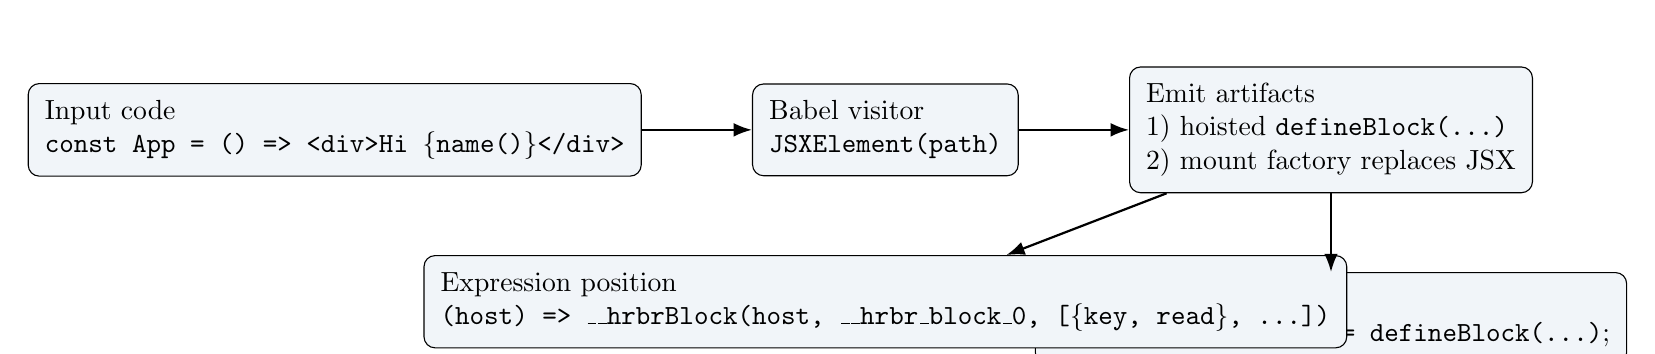
\begin{tikzpicture}[
  node distance=10mm and 14mm,
  box/.style={draw, rounded corners, align=left, inner sep=6pt, fill=RelaxLight},
  arrow/.style={-Latex, thick}
]
\node[box] (input) {Input code\\\texttt{const App = () => <div>Hi \{name()\}</div>}};
\node[box, right=of input] (visit) {Babel visitor\\\texttt{JSXElement(path)}};
\node[box, right=of visit] (emit) {Emit artifacts\\1) hoisted \texttt{defineBlock(...)}\\2) mount factory replaces JSX};

\node[box, below=of emit] (hoist) {Module scope\\\texttt{const \_\_hrbr\_block\_0 = defineBlock(...)};};
\node[box, below=of visit] (replace) {Expression position\\\texttt{(host) => \_\_hrbrBlock(host, \_\_hrbr\_block\_0, [\{key, read\}, ...])}};

\draw[arrow] (input) -- (visit);
\draw[arrow] (visit) -- (emit);
\draw[arrow] (emit) -- (hoist);
\draw[arrow] (emit) -- (replace);
\end{tikzpicture}
\end{center}

The key optimization is hoisting: the template is parsed once per module, while the mount factory runs per render/mount.

\section{Program-level state and synthesis (imports + wrappers)}

The plugin keeps per-file state variables:

\begin{itemize}
\item \texttt{needsRuntimeImport}: whether to inject \texttt{defineBlock/mountCompiledBlock}
\item \texttt{needsFallbackImport}: whether to also import \texttt{mountFallback}
\item \texttt{needsWrapper}: whether to emit the wrapper function \texttt{\_\_hrbrBlock}
\item \texttt{nextBlockId}: a counter used to generate \texttt{\_\_hrbr\_block\_0}, \texttt{\_\_hrbr\_block\_1}, ...
\item \texttt{currentFileName\/currentFileCode}: used for context-rich error messages
\end{itemize}

These are reset in the \texttt{Program.enter} visitor and materialized in \texttt{Program.exit}:

\begin{itemize}
\item \texttt{ensureRuntimeImport(programPath)} uses \texttt{unshiftContainer('body', ImportDeclaration)}.
\item \texttt{ensureWrapper(programPath)} appends \texttt{function \_\_hrbrBlock(host, def, slots) \{ return mountCompiledBlock(def, host, slots) \}}.
\end{itemize}

Implementation note: this scaffold avoids depending on Babel "types" helpers by emitting raw AST node objects.

\subsection*{Diagram: per-file state at \texttt{Program.enter/exit}}
\begin{center}
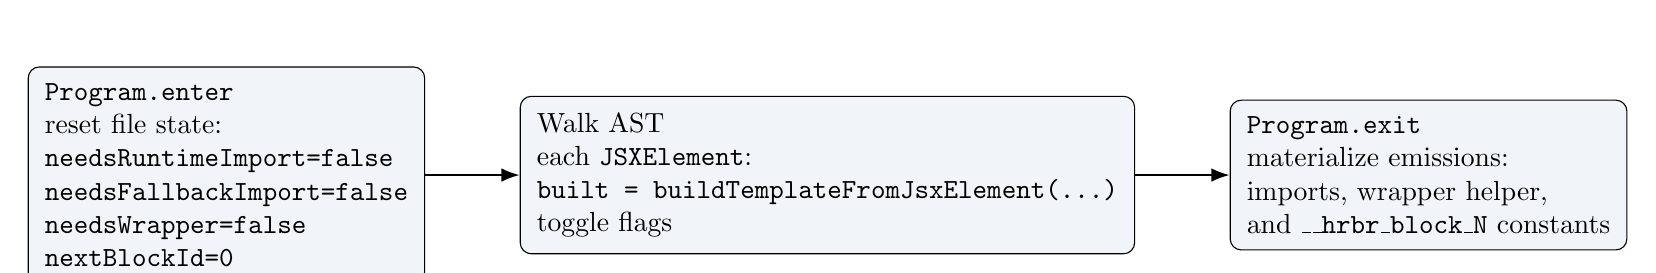
\begin{tikzpicture}[
  node distance=9mm and 12mm,
  box/.style={draw, rounded corners, align=left, inner sep=6pt, fill=RelaxLight},
  arrow/.style={-Latex, thick}
]
\node[box] (enter) {\texttt{Program.enter}\\reset file state:\\\texttt{needsRuntimeImport=false}\\\texttt{needsFallbackImport=false}\\\texttt{needsWrapper=false}\\\texttt{nextBlockId=0}};
\node[box, right=of enter] (walk) {Walk AST\\each \texttt{JSXElement}:\\\texttt{built = buildTemplateFromJsxElement(...)}\\toggle flags};
\node[box, right=of walk] (exit) {\texttt{Program.exit}\\materialize emissions:\\imports, wrapper helper,\\and \texttt{\_\_hrbr\_block\_N} constants};

\draw[arrow] (enter) -- (walk);
\draw[arrow] (walk) -- (exit);
\end{tikzpicture}
\end{center}

This structure prevents unused imports/helpers: nothing is emitted unless some subtree required it.

\subsection{Why inject at \texttt{Program.exit}?}

The plugin defers emissions until \texttt{Program.exit} so it can answer questions like:

\begin{itemize}
\item Did we ever successfully compile a block? If so, we need \texttt{defineBlock} and \texttt{mountCompiledBlock}.
\item Did any subtree route to fallback? If so, we need \texttt{mountFallback} too.
\item Did we generate a wrapper call? If so, we need to emit the wrapper function body.
\end{itemize}

This design keeps the output minimal: files that contain no transformable JSX don't get imports they don't use.

\section{The core visitor: \texttt{JSXElement(path)}}

The plugin's heart is the \texttt{JSXElement} visitor.
For each JSX element in an expression position, it calls:

\begin{quote}
\texttt{const built = buildTemplateFromJsxElement(path)}
\end{quote}

\subsection{Success path: compile into a block}

When \texttt{built} is non-null:

\begin{enumerate}
\item Mark \texttt{needsRuntimeImport = true} and \texttt{needsWrapper = true}.
\item Insert a module-scope \texttt{const \_\_hrbr\_block\_N = defineBlock(\{ templateHTML, slots \})}.
\item Replace the JSX expression with:\\
\texttt{host => \_\_hrbrBlock(host, \_\_hrbr\_block\_N, built.compiledSlots)}
\end{enumerate}

The slot objects are turned into AST literals through \texttt{literalizeSlot(slot)}.

\subsubsection{Hoisting: why \texttt{defineBlock(...)} lives at module scope}

The plugin uses \texttt{unshiftContainer('body', ...)} on the program node to emit:

\begin{quote}
	exttt{const \_\_hrbr\_block\_N = defineBlock({ templateHTML, slots })}
\end{quote}

Hoisting matters for two reasons:

\begin{itemize}
\item \textbf{Performance:} we want template parsing and slot-path validation to happen once per module, not once per render.
\item \textbf{Identity:} the mount factory will refer to a stable \texttt{\_\_hrbr\_block\_N} constant.
\end{itemize}

\subsection{Failure path: route to fallback}

When \texttt{built} is null, the plugin attempts a \emph{minimal fallback transform}.

\paragraph{Why fallback exists}

Block mode requires a stable template. Expressions that can produce different node shapes at runtime (conditionals, JSX inside expressions, etc.) must be executed by the fallback runtime, which uses the reconciler.

\subsection*{Diagram: fallback routing when template extraction fails}
\begin{center}
\begin{tikzpicture}[
  node distance=10mm and 14mm,
  box/.style={draw, rounded corners, align=left, inner sep=6pt, fill=RelaxLight},
  arrow/.style={-Latex, thick},
  decision/.style={draw, diamond, aspect=2, inner sep=2.5pt, align=center, fill=RelaxLight}
]
\node[box] (jsx) {JSX subtree\\\texttt{<div>...}};
\node[decision, right=of jsx] (ok) {Can build\\stable template?};
\node[box, above right=of ok] (block) {Block transform\\emit \texttt{defineBlock + compiledSlots}};
\node[box, below right=of ok] (fb) {Fallback transform\\emit \texttt{host => mountFallback(...)}\\\texttt{renderFn} returns specs};

\draw[arrow] (jsx) -- (ok);
\draw[arrow] (ok) -- node[midway, above] {yes} (block);
\draw[arrow] (ok) -- node[midway, below] {no} (fb);
\end{tikzpicture}
\end{center}

In other words: block mode is an optimization; fallback mode is the semantic firewall.

\paragraph{Current fallback subset}

The fallback routing in \texttt{transform.ts} is intentionally small:

\begin{itemize}
\item It only supports intrinsic lowercase root tags.
\item It only supports children that are \texttt{JSXText} or \texttt{JSXExpressionContainer}.
\item It allows only static string attributes (and ignores dynamic attrs).
\item It rejects spread attributes and event handlers.
\end{itemize}

In this subset, the plugin synthesizes a \texttt{render()} function (a closure-free data + expression composition) and emits:

\begin{quote}
\texttt{host => mountFallback(host, () => (\{ children: [spec] \}))}
\end{quote}

Each child spec contains:

\begin{itemize}
\item \texttt{create(): Element} -> creates the element and sets attributes/text
\item \texttt{patch(node)} -> updates textContent based on the latest expressions
\item optional \texttt{key} if a \texttt{key=} attribute is present
\end{itemize}

This is enough to prove the end-to-end pipeline and to connect the compiler to the fallback runtime from earlier chapters.

\subsection{Fallback synthesis: what gets captured (and what doesn't)}

The fallback compiler intentionally avoids capturing complex structures.
It builds a \texttt{renderFn} with the shape:\\
	exttt{() => ({ children: [spec] })}

Where \texttt{spec.create()} and \texttt{spec.patch(node)} both close over the user expressions.

Important implications:

\begin{itemize}
\item \textbf{Reactivity comes from runtime:} \texttt{mountFallback} re-runs \texttt{renderFn} under tracking and schedules reconciliation.
\item \textbf{This is not a general JSX renderer:} it is a deliberate minimal bridge used to validate the ``block or fallback'' architecture.
\end{itemize}

\section{Template extraction: \texttt{buildTemplateFromJsxElement()}}

The function \texttt{buildTemplateFromJsxElement()} is a best-effort compiler for a supported subset.
It returns either a full block build or \texttt{null}.

\subsection{Supported subset (today)}

In block mode, the transformer supports:

\begin{itemize}
\item intrinsic lowercase tags only (e.g. \texttt{div}, \texttt{section})
\item nested elements
\item static string attributes
\item expression attributes -> slot kinds \texttt{class/style/attr}
\item dynamic text children -> only when the expression is ``text-like''
\end{itemize}

It explicitly rejects (in block mode):

\begin{itemize}
\item event handlers (\texttt{onClick=} etc.)
\item fragments (\texttt{<>...</>})
\item non-intrinsic tags (components, capitalized)
\item spread attributes (\texttt{\{...props\}})
\end{itemize}

\subsection{How paths are computed in the Babel transform}

Like the TS prototype compiler (Chapter~\ref{ch:compiler-architecture}), this transform must produce \texttt{childNodes}-based paths.

In \texttt{renderElement(...)} the transform:

\begin{itemize}
\item keeps a per-parent counter \texttt{childState.i} that increments for each child node
\item uses \texttt{pathToHere} plus the current index to form paths like \texttt{[3,1]}
\item emits a placeholder text node (a single space) when it needs to guarantee the existence of a text node for a dynamic text slot
\end{itemize}

This is why the snapshot test shows a template that contains \emph{extra whitespace} in places where text slots are inserted. That whitespace isn't an aesthetic choice; it's a structural anchor.

\subsection{Slot keys: sequential vs location-based}

Slot keys are allocated in \texttt{allocSlotKey()}.

\begin{itemize}
\item Default: sequential keys \texttt{s0}, \texttt{s1}, ...
\item Dev mode (\texttt{stableSlotKeys=true}): keys include source location: \texttt{s\_\textless{}kind\textgreater{}\_\textless{}line\textgreater:\textless{}col\textgreater}.
\end{itemize}

This is validated in \texttt{compiler/\_\_tests\_\_/babel-transform.test.ts}.

One nuance: location-based slot keys depend on Babel preserving \texttt{loc} information and comments; this is why dev mode is framed as "debug output" rather than a semantic requirement.

\subsection{Lane pragmas: \texttt{/*@lane transition*/}}

The helper \texttt{extractLanePragmaFromExpressionContainer()} scans leading comments and looks for:

\begin{quote}
\texttt{@lane (sync|input|default|transition|idle)}
\end{quote}

If present, the emitted slot metadata includes \texttt{lane: "..."}.
The tests verify that the transformed output contains the lane strings.

\subsection{Text-like safety}

In \texttt{isTextLikeExpr()}, the transform tries to reject expressions that can yield JSX elements or otherwise change DOM structure.

Examples treated as \emph{not text-like}:

\begin{itemize}
\item returning JSX elements/fragments
\item conditionals/logicals that could yield elements (conservatively rejected)
\end{itemize}

When an expression is accepted as text-like, the transform:

\begin{itemize}
\item emits a sentinel space in the template (so a text node exists)
\item records a \texttt{text} slot pointing to that position
\item emits a compiled slot \texttt{read: () => expr}
\end{itemize}

The predicate \texttt{isTextLikeExpr(expr)} is the key safety gate.
It explicitly rejects:

\begin{itemize}
\item \texttt{JSXElement} and \texttt{JSXFragment} (obviously structural)
\item \texttt{ConditionalExpression} and \texttt{LogicalExpression} (conservatively structural for now)
\end{itemize}

This conservative choice is why the fallback e2e test uses \texttt{show() ? name() : ''} to force fallback routing: it is not considered "text-like" yet.

\section{Failure modes are part of the API}

This compiler phase aims for clarity and determinism.
Unsupported syntax produces explicit errors via \texttt{fail(path, message)} which attempts to build Babel code-frame errors.

The file \texttt{compiler/\_\_tests\_\_/babel-transform.errors.test.ts} locks in these failure modes:

\begin{itemize}
\item event handlers should throw
\item spread attributes should throw
\item fragments should throw
\item non-intrinsic tags should throw
\end{itemize}

While these errors might eventually become "route to fallback" behaviors, they're still valuable today: they prevent the compiler from silently generating templates that would be incorrect (for example, by treating an event handler like an attribute).

\section{End-to-end tests: jsdom execution proves output shape}

Two e2e suites validate that the emitted output is not just syntactically correct but \emph{runnable}.

\subsection{Block mode e2e: transformed output mounts and updates}

\texttt{compiler/\_\_tests\_\_/babel-transform.e2e-jsdom.test.ts} compiles a small component, extracts the generated \texttt{defineBlock(...)} literal and the \texttt{compiledSlots} array literal, evaluates them with \texttt{new Function(...)} and mounts the result with \texttt{mountCompiledBlock}.

The key invariant: updating a signal updates the DOM without recreating the root element.

This suite also proves a deeper property: the emitted output can be \emph{partially evaluated}.
The test extracts only the \texttt{defineBlock(...)} object literal and the compiled slots array literal, then evaluates them with \texttt{new Function}.
So the plugin isn't just emitting runnable code; it's emitting code whose pieces behave like data.

\subsection{Fallback routing e2e: structural text expression goes to \texttt{mountFallback}}

\texttt{compiler/\_\_tests\_\_/babel-transform.fallback.e2e-jsdom.test.ts} compiles an expression with a structural conditional:

\begin{quote}
\texttt{<div>\{show() ? name() : ''\}</div>}
\end{quote}

This should include \texttt{mountFallback} in output and remain reactive under signal updates.

The spec here is intentionally small:

\begin{itemize}
\item it asserts that \texttt{mountCompiledBlock} should \emph{not} be called
\item it asserts that mounting succeeds and subsequent signal changes cause updates
\item it does \emph{not} assert perfect minimal DOM operations yet
\end{itemize}

That matches the current purpose of fallback in this compiler phase: correctness-first safety for dynamic structure.

\section{What to improve next (guided by tests)}

The current transform is intentionally conservative.
The next incremental steps typically look like:

\begin{itemize}
\item add safe event slot support (mapping \texttt{onClick} to HRBR event slots)
\item support fragments by lowering them to concatenated children in block mode
\item expand fallback routing to support nested children specs (not just a single root spec)
\item improve text-like analysis so common conditionals can stay in block mode when both arms are text
\end{itemize}

The rule is always: add a targeted test first (unit + e2e), then widen syntax support.

When you widen the subset, remember the three invariants all previous chapters rely on:

\begin{itemize}
\item slot paths must match \texttt{childNodes}
\item stable mount function identity enables reuse in VDOM interop
\item fallback must remain safe when structure can change
\end{itemize}

\section{Online resources}

\begin{itemize}
\item Babel plugin authoring and visitor lifecycle:\\
\href{https://babeljs.io/docs/en/plugins}{Babel docs: plugins},\\
\href{https://babeljs.io/docs/en/babel-plugin-api}{Babel docs: plugin API}.

\item JSX AST node shapes (useful when reading \texttt{JSXElement}, \texttt{JSXText}, and \texttt{JSXExpressionContainer} visitor logic):\\
\href{https://github.com/babel/babel/blob/main/packages/babel-parser/ast/spec.md}{Babel parser AST spec}.

\item Source maps and why transforms try to preserve locations:\\
\href{https://sourcemaps.info/spec.html}{Source Map Revision 3 Proposal}.

\item ``Static template + dynamic slots" as a general pattern (useful for intuition):\\
\href{https://svelte.dev/docs/svelte/what-is-svelte}{Svelte docs: compiler-first model}.
\end{itemize}

\chapter{Devtools and instrumentation (optional)}
\label{ch:devtools}

Relax's HRBR runtime is designed to be deterministic and debuggable.
This chapter documents the small \emph{optional} devtools surface in \texttt{runtime/devtools.ts} and how the rest of the runtime reports events into it.

The design goals are:

\begin{itemize}
\item \textbf{Low overhead by default}: counters for heavyweight instrumentation (DOM ops, allocations) are disabled unless explicitly enabled.
\item \textbf{Always hookable}: events can be observed via a hook regardless of whether counting is enabled.
\item \textbf{Stable semantics}: the runtime emits a small number of event types at well-defined points.
\end{itemize}

\section{The API surface: five functions and two helpers}

All of devtools lives in \texttt{runtime/devtools.ts}.
The public API is:

\begin{itemize}
\item \texttt{setDevtoolsHook(hook | null)} -> register/unregister a global event sink
\item \texttt{getDevtoolsCounters()} -> get a defensive copy of counters
\item \texttt{resetDevtoolsCounters()} -> zero all counters
\item \texttt{setInstrumentationEnabled(boolean)} -> enable counting for expensive instrumentation
\item \texttt{isInstrumentationEnabled()} -> query the flag
\end{itemize}

And the helper emission functions used across the runtime:

\begin{itemize}
\item \texttt{emitDevtoolsEvent(event)} -> core increment + forward logic
\item \texttt{emitDomOp(op)} and \texttt{emitAlloc(kind, count?)} -> convenience wrappers
\end{itemize}

The reactivity and scheduling layers re-export these through \texttt{runtime/index.ts} so ``public HRBR'' users can import them.

\subsection*{Diagram: devtools module as a hub (hooks + counters)}
\begin{center}
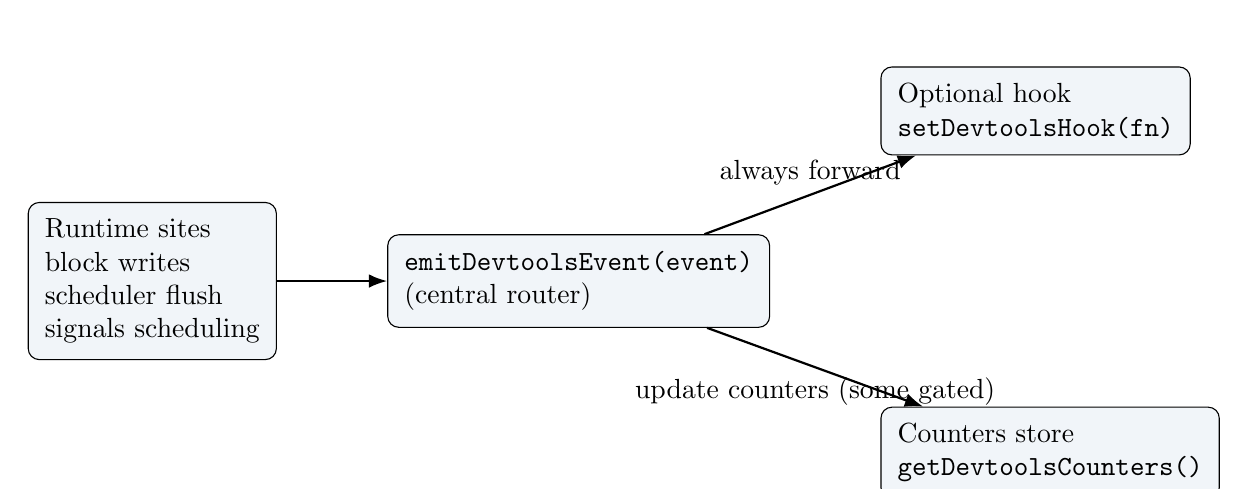
\begin{tikzpicture}[
	node distance=10mm and 14mm,
	box/.style={draw, rounded corners, align=left, inner sep=6pt, fill=RelaxLight},
	arrow/.style={-Latex, thick}
]
\node[box] (runtime) {Runtime sites\\block writes\\scheduler flush\\signals scheduling};
\node[box, right=of runtime] (emit) {\texttt{emitDevtoolsEvent(event)}\\(central router)};
\node[box, above right=of emit] (hook) {Optional hook\\\texttt{setDevtoolsHook(fn)}};
\node[box, below right=of emit] (counters) {Counters store\\\texttt{getDevtoolsCounters()}};

\draw[arrow] (runtime) -- (emit);
\draw[arrow] (emit) -- node[midway, above] {always forward} (hook);
\draw[arrow] (emit) -- node[midway, below] {update counters (some gated)} (counters);
\end{tikzpicture}
\end{center}

This captures the intent: event forwarding is always possible, while some counter updates are optional for performance.

\subsection{Tiny contract (what you can rely on)}

The devtools module is deliberately small, but it still has a stable contract:

\begin{itemize}
\item If you install a hook with \texttt{setDevtoolsHook()}, it will receive \emph{every} emitted event.
\item Counters are best-effort metrics intended for debugging/perf investigation, not correctness.
\item Expensive counters (DOM ops, allocations) are disabled by default and must be explicitly enabled.
\item \texttt{getDevtoolsCounters()} returns a copy (so the internal counter object can't be mutated externally).
\end{itemize}

\section{Event model}

Devtools events are a tagged union \texttt{DevtoolsEvent}:

\begin{itemize}
\item \texttt{slotWrite}: emitted when a block slot write is attempted
\item \texttt{scheduleComputation}: emitted when a reactive computation is scheduled
\item \texttt{flushStart} / \texttt{flushEnd(durationMs)}: emitted by the deterministic scheduler
\item \texttt{domOp(op)}: emitted by the block runtime around DOM mutations (counted only when instrumentation is enabled)
\item \texttt{alloc(kind, count?)}: emitted by allocation sites (counted only when instrumentation is enabled)
\item \texttt{patchPhase(phase, durationMs)}: emitted by the VDOM patcher to attribute time to specific patch phases
\end{itemize}

The idea is that you can build either:

\begin{itemize}
\item simple counters (the built-in ones), or
\item richer tooling (log streams, flamegraphs, dashboards) via the hook.
\end{itemize}

\section{Counters: what is tracked and when}

The internal counters live in a module-local object \texttt{\_counters}:

\begin{itemize}
\item \texttt{slotWrites}
\item \texttt{scheduledComputations}
\item \texttt{flushes}
\item \texttt{flushTimeMs}
\item \texttt{domOps} (instrumentation gated)
\item \texttt{allocs} (instrumentation gated)
\item \texttt{patchPhases} (instrumentation gated; number of patchPhase events counted)
\item \texttt{patchTimeMs} (instrumentation gated; sum of patchPhase durations)
\end{itemize}

\subsection{Defensive reads: \texttt{getDevtoolsCounters()}}

\texttt{getDevtoolsCounters()} returns \texttt{\{ \ldots\_counters \}}.
This is important: tests and users can't mutate internal state by holding onto the object.

The corresponding reset function, \texttt{resetDevtoolsCounters()}, mutates the internal object in-place. That choice keeps object identity stable for any internal references while still providing deterministic test setup.

\subsection{Why DOM ops and allocs are gated}

Counting DOM operations and allocations often requires adding emission calls in hot loops.
The devtools system separates \emph{event forwarding} from \emph{counter increments}:

\begin{itemize}
\item Events are always forwarded to the hook.
\item Counter increments for \texttt{domOp} and \texttt{alloc} only happen when \texttt{\_instrumentationEnabled} is true.
\end{itemize}

This split is implemented directly in \texttt{runtime/devtools.ts}:

\begin{itemize}
\item \texttt{emitDevtoolsEvent()} always forwards to \texttt{\_hook?.(event)}.
\item Only the \texttt{domOp} and \texttt{alloc} branches check \texttt{\_instrumentationEnabled} before touching counters.
\end{itemize}

\subsection*{Diagram: gating policy (forward always, count sometimes)}
\begin{center}
\begin{tikzpicture}[
	node distance=9mm and 12mm,
	box/.style={draw, rounded corners, align=left, inner sep=6pt, fill=RelaxLight},
	arrow/.style={-Latex, thick},
	decision/.style={draw, diamond, aspect=2, inner sep=2.5pt, align=center, fill=RelaxLight}
]
\node[box] (event) {Event created\\\texttt{\{type: 'domOp', op: ...\}}};
\node[box, right=of event] (forward) {Forward to hook\\\texttt{\_hook?.(event)}};
\node[decision, right=of forward] (enabled) {Instrumentation\\enabled?};
\node[box, above right=of enabled] (count) {Increment counters\\\texttt{domOps++}\\\texttt{allocs++}};
\node[box, below right=of enabled] (skip) {Skip counter update\\(keep overhead low)};

\draw[arrow] (event) -- (forward);
\draw[arrow] (forward) -- (enabled);
\draw[arrow] (enabled) -- node[midway, above] {yes} (count);
\draw[arrow] (enabled) -- node[midway, below] {no} (skip);
\end{tikzpicture}
\end{center}

This is the perf contract: you can always observe events, but you only pay for counting when you asked for it.

\section{Emission: increment + forward}

\texttt{emitDevtoolsEvent(event)} does two things:

\begin{enumerate}
\item updates counters based on the event type
\item forwards the event to \texttt{\_hook} if present
\end{enumerate}

In pseudo-code, the key policy is:

\begin{quote}
\texttt{always forward to hook; only count domOp/alloc when enabled}
\end{quote}

The convenience wrappers \texttt{emitDomOp()} and \texttt{emitAlloc()} add one more optimization:

\begin{itemize}
\item if instrumentation is disabled \emph{and no hook is installed}, they return immediately
\end{itemize}

This prevents needless event objects from being allocated on the hot path.

\subsection{Patch-phase measurement: a benchmark-oriented span}

Classic VDOM performance questions often require answers like:

\begin{itemize}
\item ``Is time dominated by diff traversal or DOM mutations?''
\item ``Are we spending most time reordering nodes, or updating attributes/styles/events?''
\end{itemize}

Relax's HRBR path largely avoids whole-tree diffing, but the classic VDOM path (\texttt{src/patch-dom.ts}) still benefits from targeted profiling.

For that purpose, devtools includes a tiny helper:

\begin{quote}
	\texttt{measurePatchPhase(phase, fn) -> result}
\end{quote}

It measures \texttt{fn()} using \texttt{performance.now()} (fallback \texttt{Date.now()}) and emits a \texttt{patchPhase} event with \texttt{phase} and \texttt{durationMs}.

The gating policy matches the rest of devtools:

\begin{itemize}
\item If instrumentation is disabled \emph{and} no hook is installed, \texttt{measurePatchPhase} is a no-op wrapper.
\item If a hook is installed (``streaming mode''), events flow so the benchmark harness can aggregate phase time without enabling expensive counters.
\item If instrumentation is enabled, \texttt{patchPhases} and \texttt{patchTimeMs} counters are updated.
\end{itemize}

This keeps the default runtime overhead near zero while still making deep dives possible when you ask for them.

\subsection{A subtle performance point: "no hook" short-circuit}

Notice the early return:

\begin{quote}
	\texttt{if (!enabled \&\& !hook) return}
\end{quote}

This means there are three distinct operating modes:

\begin{itemize}
\item \textbf{Default mode (recommended for production):} no hook; instrumentation disabled. Most hot-path emitters become no-ops.
\item \textbf{Streaming mode:} hook installed; instrumentation disabled. Events still flow, but counters don't track domOps/allocs.
\item \textbf{Instrumentation mode:} instrumentation enabled (hook optional). Counters track domOps/allocs.
\end{itemize}

\section{Where events come from in the runtime}

The core runtime emits events from a few key paths:

\subsection{Blocks: slot writes and DOM operations}

In \texttt{runtime/block.ts}:

\begin{itemize}
\item Every slot write emits \texttt{\{ type: 'slotWrite', slotKind, slotKey \}}.
\item Many DOM mutations are annotated with \texttt{emitDomOp('setText')}, \texttt{emitDomOp('setAttribute')}, etc.
\end{itemize}

This provides a cheap ``what changed'' signal even without full DOM diffing.

\subsubsection{Slot writes: one event per attempted update}

In \texttt{runtime/block.ts}, every slot application includes:

\begin{quote}
	\texttt{emitDevtoolsEvent(\{ type: 'slotWrite', slotKind: slot.kind, slotKey: key \})}
\end{quote}

This is intentionally emitted even when the runtime later decides to skip a DOM write (for example when values are \texttt{Object.is} equal). That makes slotWrites a measure of "reactive updates attempted" rather than "DOM updates performed".

\subsubsection{DOM operations: a vocabulary of \texttt{domOp} strings}

The block runtime calls \texttt{emitDomOp(...)} around operations like:

\begin{itemize}
\item \texttt{setText}
\item \texttt{setAttribute} / \texttt{removeAttribute}
\item \texttt{setProperty}
\item \texttt{styleSetProperty} / \texttt{styleRemoveProperty}
\item \texttt{addEventListener} / \texttt{removeEventListener}
\end{itemize}

The string payload keeps the event cheap to allocate and flexible to extend.

\subsection{Scheduler: flush timing}

In \texttt{runtime/scheduler.ts}, the flush loop emits:

\begin{itemize}
\item \texttt{flushStart} at the beginning
\item \texttt{flushEnd(durationMs)} at the end
\end{itemize}

This is the basis for simple performance dashboards.

In \texttt{runtime/scheduler.ts}, these events are emitted inside \texttt{flush(...)}:

\begin{itemize}
\item \texttt{flushStart} at the beginning
\item \texttt{flushEnd(durationMs)} at the end (duration computed using the scheduler's \texttt{now()} source)
\end{itemize}

Because the scheduler is designed to be deterministic (queues sorted by lane/priority and stable promotion rules), these timing events are also useful when you want to prove "same inputs produce the same flushing pattern".

\subsection{Signals: scheduled computations}

In \texttt{runtime/signals.ts}, scheduling a non-sync computation emits \texttt{scheduleComputation}.
The devtools counter is intentionally `how many computations were scheduled`, not `how many ran`.

The payload includes optional \texttt{name} and \texttt{lane} metadata taken from the computation object. That metadata isn't required for semantics, but it makes event streams much more useful in practice (you can group by lane or by effect name when debugging).

\section{Tests-as-spec}

There are two test files that define the intended behavior.

\subsection{\texttt{runtime/\_\_tests\_\_/devtools.test.ts}}

This suite checks two high-level properties:

\begin{itemize}
\item \textbf{slotWrites are counted} when \texttt{mountBlock()} applies initial values and when \texttt{update()} applies new values.
\item \textbf{scheduledComputations and flush metrics are counted} when the scheduler runs and when signals schedule work.
\end{itemize}

In the scheduler portion, the test uses \texttt{createScheduler({ requestFlush: (cb) => cb() })} to make flushing deterministic.

Reading this test as a contract gives you the intended semantics:

\begin{itemize}
\item Slot writes must be observed during both mount and update.
\item Scheduler flush events must be emitted even when a custom \texttt{requestFlush} runs synchronously.
\item Signal scheduling should increment a counter even if the actual effect execution happens immediately (depending on lane/batching).
\end{itemize}

\subsection{\texttt{runtime/\_\_tests\_\_/instrumentation.test.ts}}

This suite locks in the \emph{gating} behavior:

\begin{itemize}
\item without instrumentation enabled, \texttt{domOps} stays at 0 even though the runtime emits DOM op events
\item after calling \texttt{setInstrumentationEnabled(true)}, DOM-related operations increment \texttt{domOps}
\end{itemize}

This is a very important behavioral line for performance: many hot paths call \texttt{emitDomOp()} all the time, and the test documents that these calls must not inflate counters unless instrumentation is explicitly enabled.

\section{How you might use this in practice}

\subsection{Rationale: what problem are we solving?}

When people say ``devtools'' they often mean a glossy UI.
But the hard part comes first: you need a \emph{stable and cheap} stream of runtime facts.
In this repo, the HRBR runtime is fast specifically because it avoids whole-tree diffing; that also means you don't get a built-in ``diff'' you can inspect.

So the question becomes:

\begin{quote}
\emph{If the runtime doesn't diff a tree, what do we observe to debug performance and correctness?}
\end{quote}

The devtools layer answers that by emitting \emph{small, well-timed events}:

\begin{itemize}
\item A slot write attempt tells you ``reactivity wanted to change something.''
\item A DOM op tells you ``we actually touched the DOM'' (when instrumentation is enabled).
\item Scheduler flush boundaries tell you ``work was batched and committed now.''
\end{itemize}

Why it matters: these events let you debug the two hardest classes of UI problems:

\begin{itemize}
\item \textbf{Too much work:} you are doing redundant updates, thrashing the DOM, or flushing too often.
\item \textbf{Work at the wrong time:} you are flushing in a tight loop or starving lower-priority work.
\end{itemize}

The design is intentionally minimal so it stays truthful: a few counters and an event hook are much harder to accidentally ``lie'' with than a large, stateful instrumentation system.

\subsection{A tiny devtools ``panel'' in 50 lines (hook + DOM)}

The runtime doesn't ship a UI, but it gives you everything you need to build one.
Here's a minimal pattern you can paste into a demo page: install a hook, aggregate in userland, and render a tiny dashboard.

\begin{lstlisting}[language=JavaScript]
import {
	setDevtoolsHook,
	getDevtoolsCounters,
	resetDevtoolsCounters,
	setInstrumentationEnabled,
} from 'relax/hrbr'

export function installHrbrDevtoolsPanel(hostEl) {
	// Optional: enable expensive counters.
	setInstrumentationEnabled(true)
	resetDevtoolsCounters()

	const state = {
		domOpsByKind: Object.create(null),
		lastFlushDurationMs: 0,
	}

	setDevtoolsHook((e) => {
		if (e.type === 'domOp') {
			state.domOpsByKind[e.op] = (state.domOpsByKind[e.op] ?? 0) + 1
		}
		if (e.type === 'flushEnd') {
			state.lastFlushDurationMs = e.durationMs
		}
	})

	function render() {
		const c = getDevtoolsCounters()
		hostEl.innerHTML = `
			<pre>
slotWrites: ${c.slotWrites}
scheduledComputations: ${c.scheduledComputations}
flushes: ${c.flushes}
flushTimeMs: ${c.flushTimeMs}
domOps: ${c.domOps}
allocs: ${c.allocs}

lastFlushDurationMs: ${state.lastFlushDurationMs}
domOpsByKind: ${JSON.stringify(state.domOpsByKind, null, 2)}
			</pre>
		`
		requestAnimationFrame(render)
	}

	render()
	return () => setDevtoolsHook(null)
}
\end{lstlisting}

Two important details in this example are grounded in \texttt{runtime/devtools.ts}:

\begin{itemize}
\item The hook sees \emph{every} event, even if expensive counters are disabled.
\item If you don't install a hook \emph{and} you keep instrumentation disabled, hot-path emitters are designed to become no-ops.
\end{itemize}

This is why the API is split into both counters and a hook: you can build UIs without forcing the runtime to count every single thing.

\subsection{How to interpret the counters (and common misreads)}

Counters are not correctness.
They are an intentionally blunt instrument.
Here are the interpretations that match the tests:

\begin{itemize}
\item \textbf{\texttt{slotWrites}}: how many slot updates were \emph{attempted} by the block runtime.
	This includes cases where the runtime decides a DOM write is unnecessary.
\item \textbf{\texttt{domOps}}: how many DOM mutations were observed \emph{when instrumentation is enabled}.
	The instrumentation tests lock in that this must stay at 0 by default.
\item \textbf{\texttt{scheduledComputations}}: how often signals scheduled work (not necessarily how often it ran).
\item \textbf{\texttt{flushes}} and \textbf{\texttt{flushTimeMs}}: coarse scheduler batch metrics.
\end{itemize}

Common misread: ``slotWrites went up, therefore DOM changed.''
Not necessarily.
In this runtime, slotWrites measure how often reactivity \emph{wanted} to update; domOps measure how often the runtime actually mutated the DOM (and only when the expensive counters are enabled).

\subsection{A tiny contract you can build tooling around}

If you want to build real tooling (like a profiler timeline), define your own minimal contract on top of the hook:

\begin{itemize}
\item Treat \texttt{flushStart} / \texttt{flushEnd} as a bracket for ``commit work''.
\item Count \texttt{domOp} events inside that bracket to get ``DOM work per flush''.
\item Group \texttt{scheduleComputation} by lane to visualize priority.
\end{itemize}

This is deliberately similar to the idea of tracing spans, but implemented with a tiny custom event union.
If you want the conceptual background, see OpenTelemetry's overview:
\href{https://opentelemetry.io/docs/what-is-opentelemetry/}{https://opentelemetry.io/docs/what-is-opentelemetry/}.

\section{Exercises (tests-first)}

\begin{enumerate}
\item \textbf{Write a test that proves the ``streaming mode'' behavior:}
			install a hook, keep instrumentation disabled, trigger a block update, and assert that you receive \texttt{domOp} events while \texttt{getDevtoolsCounters().domOps} remains 0.
			(Hint: this should be an addition to \texttt{runtime/\_\_tests\_\_/instrumentation.test.ts}.)

\item \textbf{Build a per-op counter:}
			implement a tiny helper \texttt{createDomOpsHistogram()} that installs a hook and keeps a histogram \texttt{\{ [op]: count \}}.
			Prove in a test that \texttt{setText} happens during a text slot update.

\item \textbf{Add a new event type (safely):}
			add an optional \texttt{flushBudgetMs} field to \texttt{flushStart} (or introduce a new event) and thread it from the scheduler.
			Update the tests to lock in the behavior.
			If you can't update all call sites cleanly, you're changing the contract too aggressively.
\end{enumerate}

Two common patterns:

\begin{itemize}
\item \textbf{Counters dashboard}: poll \texttt{getDevtoolsCounters()} and display deltas per second.
\item \textbf{Event stream}: set a hook via \texttt{setDevtoolsHook((e) => \{ ... \})} and record or filter events.
\end{itemize}

A practical rule of thumb:

\begin{itemize}
\item enable instrumentation only in debug builds or perf investigations
\item leave it off in production unless you have a carefully designed sampling strategy
\end{itemize}

\subsection{A simple pattern: hook + manual aggregation}

If you want detailed breakdowns without touching the built-in counters, install a hook and aggregate in userland:

\begin{itemize}
\item Count per-domain domOps (e.g. \texttt{setText} vs \texttt{setAttribute})
\item Track flush durations into histograms
\item Group schedule events by lane
\end{itemize}

This works even when instrumentation is disabled, because the hook still receives events.

\section{Online resources}

\begin{itemize}
\item Performance measurement pitfalls and best practices (timers, main-thread work, long tasks):\\
\href{https://web.dev/articles/rail}{web.dev: RAIL performance model},\\
\href{https://developer.mozilla.org/en-US/docs/Web/API/Performance/now}{MDN: \texttt{performance.now()}}.

\item Observability patterns for UI runtimes (profilers, tracing, counters):\\
\href{https://opentelemetry.io/docs/what-is-opentelemetry/}{OpenTelemetry: overview}.

\item Source maps and error locations are why devtools often care about source positions:\\
\href{https://sourcemaps.info/spec.html}{Source Map Revision 3 Proposal}.
\end{itemize}

\chapter{Benchmarks methodology (repeatability + fairness)}
\label{ch:benchmarks}

Benchmarks are where performance stories can go wrong fast.
This chapter documents Relax's benchmark harness under \texttt{benchmarks/} and the methodology guidelines captured in \texttt{docs/benchmarks.md}.

The core goals are:

\begin{itemize}
\item \textbf{Repeatability}: seeded randomness, stable profiles, and a clear warmup/measure separation.
\item \textbf{Fairness}: compare like-for-like work (same DOM outcomes, similar update patterns), and control build modes (dev vs prod).
\item \textbf{Interpretability}: report metrics that explain tail latency (p95) and not just averages.
\end{itemize}

\section{Benchmarks run in a real browser}

The harness is designed to run in a browser environment:

\begin{itemize}
\item Uses \texttt{requestAnimationFrame} to align work with frames.
\item Uses \texttt{performance.now()} for timing.
\item Bundles through Rollup configs that target \texttt{browser: true}.
\end{itemize}

See \texttt{benchmarks/index.html} and the entry script \texttt{benchmarks/main.ts}.

\subsection{A small but important detail: Node/jsdom fallback exists}

The harness is designed for browsers first, but \texttt{benchmarks/harness.ts} contains a compatibility fallback:

\begin{itemize}
\item \texttt{now()} prefers \texttt{performance.now()} but falls back to \texttt{Date.now()}.
\item \texttt{nextFrame()} prefers \texttt{requestAnimationFrame} but falls back to \texttt{setTimeout(..., 16)}.
\end{itemize}

This is \emph{not} intended to make Node-based benchmarking ``accurate''. It's there so that small smoke runs and tooling can still function in non-browser environments.

\section{The harness contract}

The core harness is \texttt{benchmarks/harness.ts}.

\subsection{Benchmark case shape}

A benchmark case is a \texttt{BenchmarkCase}:

\begin{itemize}
\item \texttt{name}: stable identifier for reporting
\item \texttt{setup(host)}: returns a controller with\newline
  \texttt{tick()} -> perform one unit of work\newline
  \texttt{teardown()} -> clean up resources and DOM
\item optional \texttt{commit()}: a barrier that resolves only once the framework has committed for the tick
\end{itemize}

The \texttt{commit()} hook is how the harness stays fair across frameworks that batch work differently (e.g. React flush/paint boundaries).

\subsection{Tiny contract for a fair \texttt{BenchmarkCase}}

To keep comparisons honest, the benchmark cases should follow a simple contract:

\begin{itemize}
\item \texttt{tick()} should perform one repeatable unit of work and avoid random extra allocations.
\item \texttt{teardown()} must remove event handlers / timers / subscriptions (avoid cross-case leaks).
\item If a framework batches updates asynchronously, provide \texttt{commit()} that resolves after work is actually committed.
\end{itemize}

\subsection{Warmup vs measure windows}

\texttt{runBenchmark()} splits execution into two windows:

\begin{itemize}
\item \textbf{Warmup frames} (default 30): let JIT, memoization, layout caching, and internal queues settle.
\item \textbf{Measure frames} (default 120): record per-tick durations.
\end{itemize}

Implementation details in \texttt{runBenchmark()}:

\begin{itemize}
\item For each tick: await \texttt{nextFrame()} , record \texttt{t0} , run \texttt{tick()} , await \texttt{commit()} , compute \texttt{dt}.
\item A \textbf{frame drop} is counted when \texttt{dt > frameBudgetMs} (default 16.7ms).
\end{itemize}

\subsection{Reported metrics: avg + p95 + drops}

The harness reports:

\begin{itemize}
\item \texttt{avgMs} , average time per tick
\item \texttt{p95Ms} , 95th percentile tick time (tail latency)
\item \texttt{frameDrops} , number of frames over budget
\end{itemize}

Percentiles are computed on sorted samples with a simple index selection.
This is good enough for stable comparisons at the harness scale.

The harness computes p95 with:\\
	exttt{idx = floor(p * (n - 1))} (clamped).
This is a simple deterministic estimator, which is a feature here: the same sample list always produces the same percentile.

\section{Profiles and seeded runs}

Repeatability relies on standard profiles and seeded randomness.

\subsection{Profiles via URL parameters}

The profile parser lives in \texttt{benchmarks/profile.ts}.

It reads query params from \texttt{benchmarks/index.html}:

\begin{itemize}
\item \texttt{profile}: \texttt{quick | default | stress}
\item \texttt{seed}: integer seed for randomized update patterns
\item \texttt{warmup}, \texttt{frames}, \texttt{budget}: overrides for fine-grained control
\end{itemize}

Defaults are intentionally ``reasonable and stable'' for local runs.

Implementation note: the profile parser clamps overrides to avoid accidental runaway configurations:

\begin{itemize}
\item \texttt{warmup} is clamped to \texttt{[0, 10000]}
\item \texttt{frames} is clamped to \texttt{[1, 100000]}
\end{itemize}

Seed values are forced into uint32 range using \texttt{>>> 0}, which keeps the PRNG behavior consistent.

\subsection{Seeded RNG}

Randomized patterns (e.g. which list indices change each tick) should be deterministic.
Benchmark code uses a seeded RNG in \texttt{benchmarks/rng.ts}.

A key methodology rule: the seed must be part of the report output so results can be reproduced.

The benchmark RNG implementation is \texttt{Mulberry32} (\texttt{benchmarks/rng.ts}). It is simple, fast, and deterministic---perfect for selecting indices or toggling boolean flags in a way that remains repeatable across runs.

\section{The benchmark runner UI}

The main entrypoint \texttt{benchmarks/main.ts} wires a button click to sequential benchmark runs.

Key details:

\begin{itemize}
\item It resets \texttt{host.innerHTML = ''} between runs so each case starts clean.
\item It prints formatted results to a \texttt{<pre>}.
\item It runs both HRBR and VDOM variants, and includes adapters for React/Solid.
\end{itemize}

Because different frameworks have different setup/teardown costs, the harness keeps the per-tick loop stable and encourages cases to isolate the steady-state behavior.

\subsection{Why \texttt{host.innerHTML = ''} between runs matters}

Clearing between runs gives you two strong properties:

\begin{itemize}
\item \textbf{Isolation:} DOM nodes and event listeners from a previous framework/case do not bleed into the next.
\item \textbf{Repeatability:} each case starts from the same initial DOM shape.
\end{itemize}

This is also why safe \texttt{teardown()} behavior is part of the case contract: the harness clears DOM, but frameworks may have timers/schedulers that need explicit disposal.

\section{Cases: what they measure}

Cases live under \texttt{benchmarks/cases/}.
The intent is to cover:

\begin{itemize}
\item \textbf{Pure text throughput}: \texttt{text-1m}
\item \textbf{Large lists with sparse updates}: \texttt{list-10k-1pct}
\item \textbf{Many small components/widgets}: \texttt{widgets-200}
\item Extra comparisons in \texttt{cases/more.ts}
\end{itemize}

Important fairness guideline: each case should produce the same DOM output across frameworks (or as close as is reasonable).

\subsection{Case study: \texttt{text-1m}}

In \texttt{benchmarks/cases/text-1m.ts}, the HRBR variant builds the smallest possible compiled block:

\begin{itemize}
\item \texttt{templateHTML: `<div><span> </span></div>`} includes an explicit space so there is a real text node.
\item Slot path \texttt{[0,0]} means: root \texttt{<div>} child 0 is \texttt{<span>}, and its child 0 is the \texttt{Text} node.
\item \texttt{tick()} updates a signal in chunks of \texttt{10,000} so work remains frame-visible.
\end{itemize}

This isn't a ``real app'' workload, but it is an excellent microbenchmark for measuring pure slot-write throughput.

\subsection{Case study: \texttt{list-10k-1pct}}

In \texttt{benchmarks/cases/list-10k-1pct.ts}, the cases delegate to example mount helpers:

\begin{itemize}
\item HRBR: \texttt{mountList10k1pctHRBR(host, 10000)}
\item VDOM: \texttt{mountList10k1pctVDOM(host, 10000)}
\end{itemize}

The contract is the same for both: return a controller with \texttt{update1pct()} and \texttt{dispose()}.
Methodologically, that matters: both implementations are being asked to do the same "one tick" of work.

\section{Build modes matter (dev vs prod)}

Some frameworks change scheduling and checks based on \texttt{process\.env\.NODE\_ENV}.
The benchmark Rollup config sets this value at bundle time.

\begin{itemize}
\item Rollup config: \texttt{rollup.benchmarks.config.mjs}
\item It uses \texttt{@rollup/plugin-replace} to define \texttt{process.env.NODE\_ENV}.
\end{itemize}

NPM scripts in \texttt{package.json} expose common modes:

\begin{itemize}
\item \texttt{build:bench:dev}
\item \texttt{build:bench:prod}
\end{itemize}

To be fair, comparisons should run with comparable modes (usually prod vs prod).

\subsection{What the Rollup configs actually do}

The benchmark bundles are built through two rollup configs:

\begin{itemize}
\item \texttt{rollup.benchmarks.config.mjs} (full UI runner)
\item \texttt{rollup.benchmarks.smoke.config.mjs} (perf-smoke gate)
\end{itemize}

Both use \texttt{@rollup/plugin-replace} to inject:\\
	exttt{process.env.NODE\_ENV = 'production'} by default.

This matters for fairness because some libraries (notably React) perform extra checks and different scheduling policies in development builds.

\section{Perf smoke (CI-friendly)}

For CI and ``obvious regression'' detection, the repo includes a reduced entry:

\begin{itemize}
\item \texttt{benchmarks/perf-smoke.ts}
\item \texttt{benchmarks/perf-smoke.html}
\end{itemize}

It builds via \texttt{rollup.benchmarks.smoke.config.mjs} into \texttt{benchmarks/dist-smoke/}.

\subsection{What perf-smoke is actually specifying}

You can read \texttt{benchmarks/perf-smoke.ts} as an executable specification of the harness:

\begin{itemize}
\item it obtains a profile via \texttt{getBenchmarkProfile()}
\item it forces short defaults unless overridden (default profile becomes \texttt{quick})
\item it runs a small fixed set of cases (currently \texttt{text-1m} and \texttt{list-10k-1pct}, HRBR variants)
\item it emits a JSON report that includes profile, timestamp, and result rows
\item it enforces very wide thresholds to catch catastrophic regressions
\end{itemize}

Even though this isn't a Vitest file, it plays the same role as tests in earlier chapters: it defines what "performance sanity" means for this repository.

\subsection{Why the thresholds are wide}

\texttt{perf-smoke.ts} prints a JSON report to \texttt{console.log} and then checks very wide thresholds:

\begin{itemize}
\item fail only when \texttt{avgMs > 250} or \texttt{p95Ms > 500}
\end{itemize}

This is intentional: CI machines are noisy.
The smoke test is designed to catch catastrophic regressions (infinite loops, accidental \(\mathcal{O}(n^2)\) behavior), not micro-optimizations.
This is also why the gate uses two different lenses:

\begin{itemize}
\item \texttt{avgMs}: for sustained runaway behavior
\item \texttt{p95Ms}: for severe tail latency spikes
\end{itemize}

Tail latency matters because user experience is dominated by occasional slow frames.

\section{Instrumentation and benchmarks: keep them separate}

Optional runtime instrumentation exists in \texttt{runtime/devtools.ts} (Chapter~\ref{ch:devtools}).

Methodology rule: keep instrumentation disabled during benchmarks unless you are explicitly measuring it.
Otherwise, the measurement includes the measurement.

In practice, if you want to correlate benchmark results with DOM op counts:

\begin{itemize}
\item run once with instrumentation off to measure baseline
\item run again with instrumentation enabled (and accept the overhead) to measure the profile of operations
\end{itemize}

Comparing these two runs helps you understand whether a regression is dominated by DOM work, scheduling, or allocation overhead.

\section{Checklist: how to run a fair comparison}

A practical checklist grounded in this repo's structure:

\begin{enumerate}
\item Build benchmark bundle in a known mode (dev or prod) and record it.
\item Use a named profile (quick/default/stress) so warmup and frames are consistent.
\item Fix a seed and include it in the report.
\item Run multiple times and compare distributions (p95 and drops), not just averages.
\item If a result looks surprising, isolate the case and profile it (browser performance tools).
\end{enumerate}

\section{Online resources}

\begin{itemize}
\item Measuring performance in the browser and why alternatives to \texttt{Date.now()} matter:\\
\href{https://developer.mozilla.org/en-US/docs/Web/API/Performance/now}{MDN: \texttt{performance.now()}}.

\item About frame budgets and why 16.7ms is the common baseline:\\
\href{https://web.dev/articles/rendering-performance}{web.dev: rendering performance}.

\item Why warmup matters (JIT, inline caches, tiered compilation):\\
\href{https://v8.dev/blog}{V8 blog (background on optimization and warmup effects)}.

\item Percentiles and tail latency as a reporting best practice:\\
\href{https://en.wikipedia.org/wiki/Percentile}{Wikipedia: percentile},\\
\href{https://research.google/pubs/pub40801/}{Google SRE: tail latency (The Tail at Scale)}.

\item General benchmark hygiene and common pitfalls:\\
\href{https://benchmarking.sites/}{benchmarking.sites (community notes)}.
\end{itemize}

\chapter{Release-quality discipline: tests, typecheck, lint, builds}
\label{ch:release-quality}

This chapter is about the habits that make a codebase shippable.
Relax is a teaching framework, but it also treats its test suite as an executable spec and its build pipeline as part of correctness.

The goal of this chapter is not to list commands---it's to explain \emph{why} each quality gate exists, what it catches, and how to debug failures without guessing.

If you only remember one thing: each gate is a different lens on correctness.
Typecheck defends your \emph{data model}, lint defends your \emph{human factors} (consistency and obvious mistakes), tests defend your \emph{observable behavior}, and builds defend your \emph{published artifact}.

\section{The quality-gates contract}

A ``release-quality'' change in this repo is expected to be green on:

\begin{itemize}
\item \textbf{Typecheck}: TypeScript compilation with \texttt{--noEmit}
\item \textbf{Lint}: ESLint rules for consistency and obvious mistakes
\item \textbf{Unit/integration tests}: Vitest (jsdom)
\item \textbf{Build}: Rollup bundles for ESM + CJS, plus type bundle generation on publish
\end{itemize}

\section*{Diagram: quality gates as a pipeline}
\begin{center}
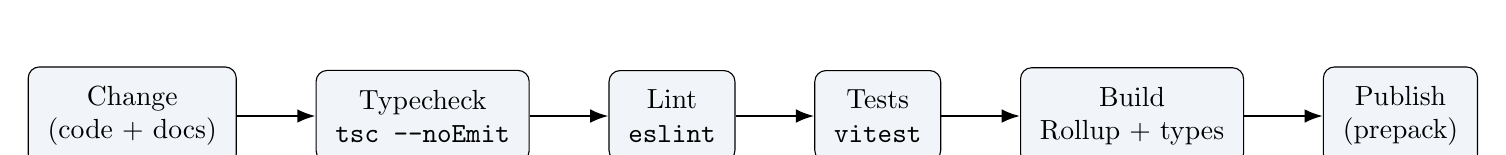
\begin{tikzpicture}[
	node distance=8mm and 10mm,
	box/.style={draw, rounded corners, align=center, inner sep=7pt, fill=RelaxLight},
	arrow/.style={-Latex, thick}
]
\node[box] (change) {Change\\(code + docs)};
\node[box, right=of change] (type) {Typecheck\\\texttt{tsc --noEmit}};
\node[box, right=of type] (lint) {Lint\\\texttt{eslint}};
\node[box, right=of lint] (test) {Tests\\\texttt{vitest}};
\node[box, right=of test] (build) {Build\\Rollup + types};
\node[box, right=of build] (ship) {Publish\\(prepack)};

\draw[arrow] (change) -- (type);
\draw[arrow] (type) -- (lint);
\draw[arrow] (lint) -- (test);
\draw[arrow] (test) -- (build);
\draw[arrow] (build) -- (ship);
\end{tikzpicture}
\end{center}

This diagram is intentionally linear. In practice you often run these in parallel locally, but conceptually each step answers a different question: ``Do the types hold?'', ``Is the diff readable?'', ``Is the behavior correct?'', and ``Is the published artifact correct?''

These are not redundant; they fail on different classes of bugs.

\subsection{A tiny contract (inputs, outputs, failure modes)}

It helps to think about the pipeline as a function that takes a working tree and returns publishable artifacts:

\begin{itemize}
\item \textbf{Input}: TypeScript source under \texttt{src/}, plus experimental surfaces under \texttt{runtime/}, \texttt{compiler/}, and the TSX runtime under \texttt{relax-jsx/}.
\item \textbf{Output}: compiled JS bundles in \texttt{dist/esm/} and \texttt{dist/cjs/} and a declaration bundle in \texttt{dist-types/}.
\item \textbf{Success}: consumers can import from the package \texttt{exports} map and get the runtime semantics the tests describe.
\item \textbf{Failure modes}: ``works in tests'' but fails to typecheck; ``works locally'' but fails to bundle; ``bundles'' but exports the wrong files.
\end{itemize}

\section{Typecheck: make illegal states unrepresentable}

The repo's primary TypeScript config is \texttt{tsconfig.json}.
A few settings worth noticing:

\begin{itemize}
\item \texttt{strict: true} --- the baseline.
\item \texttt{noUncheckedIndexedAccess: true} --- forces you to handle missing keys.
\item \texttt{exactOptionalPropertyTypes: true} --- optional means ``may be absent'', not ``may be undefined''.
\item \texttt{jsx: react-jsx} and \texttt{jsxImportSource: relax-jsx} --- enables the TSX layer.
\end{itemize}

Two other settings are quietly important for how the codebase is built and consumed:

\begin{itemize}
\item \texttt{moduleResolution: Bundler}: TypeScript resolves imports similarly to modern bundlers.
In practice, this aligns the typechecker with how Rollup (and consumer bundlers) will interpret ESM.
\item \texttt{paths} for \texttt{relax-jsx}: TS can typecheck TSX code that imports the JSX runtime via the virtual specifier \texttt{relax-jsx}.
This is mirrored on the test side by the Vitest alias for \texttt{relax-jsx}.
\end{itemize}

The \texttt{typecheck} script (in \texttt{package.json}) runs:

\begin{quote}
\texttt{tsc -p tsconfig.json --noEmit}
\end{quote}

\section*{Diagram: why multiple tsconfig files exist}
\begin{center}
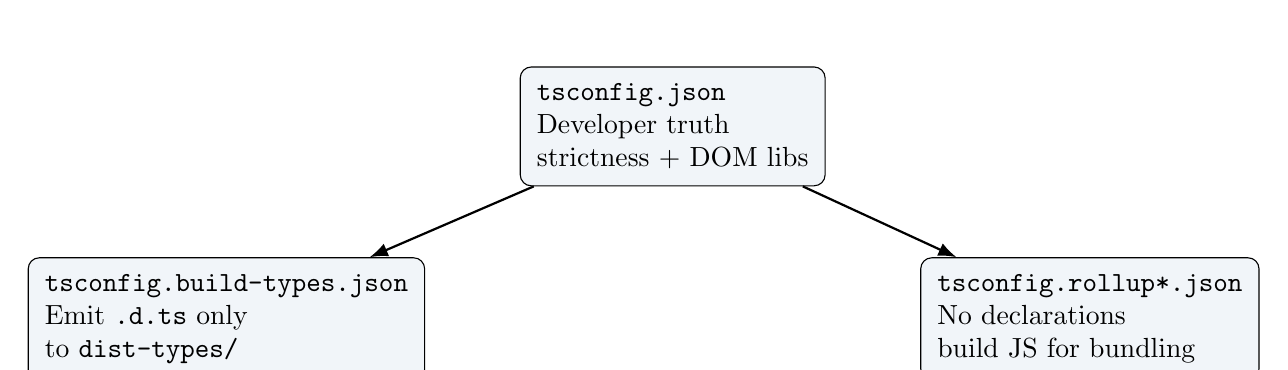
\begin{tikzpicture}[
	node distance=9mm and 12mm,
	box/.style={draw, rounded corners, align=left, inner sep=6pt, fill=RelaxLight},
	arrow/.style={-Latex, thick}
]
\node[box] (base) {\texttt{tsconfig.json}\\Developer truth\\strictness + DOM libs};
\node[box, below left=of base] (types) {\texttt{tsconfig.build-types.json}\\Emit \texttt{.d.ts} only\\to \texttt{dist-types/}};
\node[box, below right=of base] (rollup) {\texttt{tsconfig.rollup*.json}\\No declarations\\build JS for bundling};

\draw[arrow] (base) -- (types);
\draw[arrow] (base) -- (rollup);
\end{tikzpicture}
\end{center}

\subsection{Common typecheck failures (and how to debug)}

\begin{itemize}
\item \textbf{Indexing errors}: caused by \texttt{noUncheckedIndexedAccess}. Fix by narrowing or checking bounds.
\item \textbf{Optional property mismatches}: caused by \texttt{exactOptionalPropertyTypes}. Fix by removing explicit \texttt{undefined} assignments or changing types.
\item \textbf{DOM typing issues in tests}: Vitest uses jsdom; make sure \texttt{lib: ["DOM"]} is present (it is).
\end{itemize}

\subsection{Why there are multiple \texttt{tsconfig} files}

This repo uses a small family of configs to keep responsibilities separate:

\begin{itemize}
\item \texttt{tsconfig.json}: the ``truth'' for developer typechecking.
It enables declarations and maps, targets modern JavaScript (\texttt{ES2022}), and includes the DOM library.
\item \texttt{tsconfig.build-types.json}: extends the base config but turns on \emph{declaration-only} emit.
This produces the publishable \texttt{.d.ts} surface under \texttt{dist-types/}.
\item \texttt{tsconfig.rollup.json} and \texttt{tsconfig.rollup.cjs.json}: extend the base config but disable declaration emission.
These exist to keep Rollup builds focused on JavaScript output (ESM to \texttt{dist/esm/}, CJS to \texttt{dist/cjs/}) without creating duplicate \texttt{.d.ts} trees.
\end{itemize}

This split is release discipline in practice: build tooling stays fast and predictable, while types remain a first-class published artifact.

\section{Lint: keep the surface area consistent}

Lint config lives in \texttt{eslint.config.mjs}.
It uses the ESLint 9 flat config model and \texttt{@eslint/js} recommended rules.

The lint scripts are:

\begin{itemize}
\item \texttt{npm run lint} --- runs eslint on \texttt{src}
\item \texttt{npm run lint:fix} --- applies safe auto-fixes
\end{itemize}

Note: linting only \texttt{src} is a choice. HRBR runtime and compiler code are primarily guarded by tests and typecheck, but could be added to lint scope later.

\subsection{What lint catches that typecheck doesn't}

TypeScript proves things about types, but lint is often better at catching:

\begin{itemize}
\item accidental unused variables or imports
\item inconsistent patterns that make reviews harder
\item ``looks correct'' code that has a known foot-gun shape
\end{itemize}

Even with a mostly-recommended ESLint config, getting a clean lint run is part of keeping diffs small and reviewable.

\section{Tests: executable specs with jsdom}

All tests use Vitest (see \texttt{vitest.config.js}).
The environment is \texttt{jsdom}, which means:

\begin{itemize}
\item DOM APIs are available (document, elements, events)
\item you can test DOM manipulation deterministically without a real browser
\end{itemize}

Test inclusion patterns:

\begin{itemize}
\item \texttt{**/\_\_tests\_\_/**/*.test.ts}
\item \texttt{**/\_\_tests\_\_/**/*.test.tsx}
\end{itemize}

\subsection{The test suite structure}

This repo uses tests in three roles:

\begin{itemize}
\item \textbf{Unit tests}: small functions like diffs and helpers.
\item \textbf{Integration tests}: end-to-end flows (mount $\to$ patch $\to$ destroy, SSR $\to$ hydrate, compiler $\to$ mount).
\item \textbf{Property/fuzz tests}: seeded tests that exercise many update sequences (e.g. reconciler and signals).
\end{itemize}

If you change invariants (like reconciliation semantics), expect to update both unit tests and fuzz oracles.

\subsection{Tests-as-spec example: TSX wiring}

The TSX layer is a good example of how ``typecheck + tests'' combine into a stronger guarantee.
The typechecker is configured to understand TSX (\texttt{jsx: react-jsx} and \texttt{jsxImportSource: relax-jsx}), but tests still need to verify the \emph{runtime} behavior.

In \texttt{src/\_\_tests\_\_/jsx-tsx.test.ts}, the test sets up a host element in jsdom, runs an example, and asserts on the resulting HTML:

\begin{itemize}
\item it writes \texttt{<div id="app"></div>} into \texttt{document.body}
\item it locates the host element and passes it into \texttt{runHelloExample}
\item it asserts that the returned HTML matches \texttt{<div class="hello">Hello Relax</div>}
\end{itemize}

The important release-quality point is the scope of the guarantee:
this test doesn't just say ``TSX compiles''---it says ``the TSX runtime integrates with the DOM mounting layer and produces the expected structure''.

\subsection{Debugging failing tests (a workflow)}

A practical workflow:

\begin{enumerate}
\item Re-run only the failing file (Vitest supports file targeting; use the repo scripts).
\item Read the failure output and find which invariant changed.
\item Locate the corresponding runtime function and its other tests.
\item Add a minimal regression test that isolates the bug.
\item Only then, fix the implementation and re-run the focused test.
\end{enumerate}

When failures are timing-related (scheduler, signals), prefer deterministic schedulers and explicit ticking (the repo already uses this pattern).

\subsection{What to do when a test failure seems ``impossible''}

The fastest way to debug tough failures is to make the implicit invariant explicit:

\begin{enumerate}
\item Find the smallest assertion that fails.
\item Name the invariant in one sentence (e.g. ``patch preserves node identity when keys and tag match'').
\item Search for other tests that mention the same concept.
\item Read the corresponding implementation with the invariant in mind.
\end{enumerate}

This avoids the common trap of chasing symptoms across unrelated modules.

\section{Builds: ESM, CJS, and types}

Relax ships multiple entrypoints (see \texttt{package.json} \texttt{exports}):

\begin{itemize}
\item \texttt{"."} --- the VDOM library
\item \texttt{"./hrbr"} --- experimental HRBR runtime
\item \texttt{"./compiler"} --- experimental compiler
\end{itemize}

Rollup builds:

\begin{itemize}
\item ESM: \texttt{rollup.config.mjs} -> \texttt{dist/esm/}
\item CJS: \texttt{rollup.config.cjs.mjs} -> \texttt{dist/cjs/}
\end{itemize}

Type declaration builds:

\begin{itemize}
\item \texttt{npm run build:types} uses \texttt{tsconfig.build-types.json} (emit declarations only)
\item \texttt{npm run prepack} runs both JS builds and types before publishing
\end{itemize}

\subsection{Why builds are a quality gate}

A green test suite doesn't guarantee:

\begin{itemize}
\item exports are correct
\item bundling doesn't pull in unexpected dependencies
\item generated output is structurally valid for consumers
\end{itemize}

For example, the compiler bundle is large; build output sizes help you notice unexpected growth.

\subsection{Build discipline: match \texttt{exports} to outputs}

From \texttt{package.json}, Relax publishes multiple entry points (\texttt{"."}, \texttt{"./hrbr"}, \texttt{"./compiler"}).
Release discipline means each export must be correct in three dimensions:

\begin{itemize}
\item \textbf{ESM path} points at something in \texttt{dist/esm/}
\item \textbf{CJS path} points at something in \texttt{dist/cjs/} (with \texttt{.cjs} entry file names)
\item \textbf{Types path} points at something in \texttt{dist-types/}
\end{itemize}

It's easy to accidentally break this mapping when renaming files, changing entry points, or restructuring module boundaries.
That is why \texttt{prepack} builds both JS bundles and types before publish.

\section*{Diagram: package exports must match ESM, CJS, and types}
\begin{center}
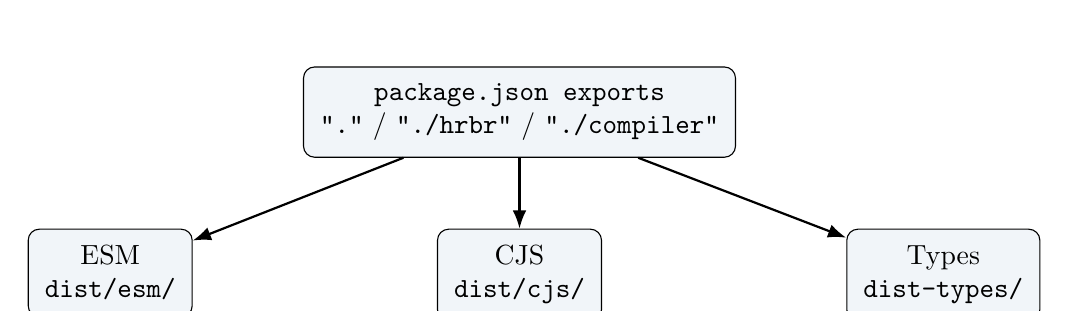
\begin{tikzpicture}[
	node distance=9mm and 14mm,
	box/.style={draw, rounded corners, align=center, inner sep=6pt, fill=RelaxLight},
	arrow/.style={-Latex, thick}
]
\node[box] (exports) {\texttt{package.json exports}\\\texttt{"."} / \texttt{"./hrbr"} / \texttt{"./compiler"}};

\node[box, below left=of exports] (esm) {ESM\\\texttt{dist/esm/}};
\node[box, below=of exports] (cjs) {CJS\\\texttt{dist/cjs/}};
\node[box, below right=of exports] (types) {Types\\\texttt{dist-types/}};

\draw[arrow] (exports) -- (esm);
\draw[arrow] (exports) -- (cjs);
\draw[arrow] (exports) -- (types);
\end{tikzpicture}
\end{center}

\section{Release checklist (practical)}

A minimal release checklist aligned with this repo:

\begin{enumerate}
\item \textbf{Typecheck}: ensure TS still models your invariants.
\item \textbf{Lint}: ensure code style and basic safety checks pass.
\item \textbf{Tests}: run the suite; if you're changing HRBR internals, keep an eye on fuzz determinism.
\item \textbf{Build}: confirm ESM + CJS outputs compile.
\item \textbf{Bench smoke (optional but recommended)}: \texttt{build:bench:smoke} to catch catastrophic perf regressions.
\end{enumerate}

\section{Evidence from this repo}

This chapter is grounded in real scripts and configs:

\begin{itemize}
\item \texttt{package.json} scripts: \texttt{typecheck}, \texttt{lint}, \texttt{test}, \texttt{build}, \texttt{prepack}
\item \texttt{vitest.config.js} (jsdom environment)
\item \texttt{eslint.config.mjs} (flat config)
\item Rollup configs for bundling
\item TypeScript configs for declaration and rollup builds
\end{itemize}

In the next section of the book (appendices), we'll turn these practices into a learner-friendly ``build it from scratch'' checklist and a test-reading guide.

\section{Online resources}

These references mirror the key moving parts in this chapter:

\begin{itemize}
\item TypeScript \texttt{tsconfig} reference (compiler options, strictness flags):
\href{https://www.typescriptlang.org/tsconfig}{https://www.typescriptlang.org/tsconfig}
\item \texttt{exactOptionalPropertyTypes} (why ``optional'' is not the same as ``possibly undefined''):
\href{https://www.typescriptlang.org/tsconfig#exactOptionalPropertyTypes}{https://www.typescriptlang.org/tsconfig\#exactOptionalPropertyTypes}
\item \texttt{noUncheckedIndexedAccess} (making missing keys explicit):
\href{https://www.typescriptlang.org/tsconfig#noUncheckedIndexedAccess}{https://www.typescriptlang.org/tsconfig\#noUncheckedIndexedAccess}
\item TypeScript JSX / \texttt{jsxImportSource}:
\href{https://www.typescriptlang.org/docs/handbook/jsx.html}{https://www.typescriptlang.org/docs/handbook/jsx.html}
\item ESLint flat config (ESLint 9+):
\href{https://eslint.org/docs/latest/use/configure/configuration-files}{https://eslint.org/docs/latest/use/configure/configuration-files}
\item Vitest docs (jsdom environment, include patterns, reporters):
\href{https://vitest.dev/guide/}{https://vitest.dev/guide/}
\item jsdom project (what it simulates and what it doesn't):
\href{https://github.com/jsdom/jsdom}{https://github.com/jsdom/jsdom}
\item Rollup configuration and multi-entry builds:
\href{https://rollupjs.org/configuration-options/}{https://rollupjs.org/configuration-options/}
\item Node.js \texttt{package.json} \texttt{exports} field (how entry points are resolved):
\href{https://nodejs.org/api/packages.html#exports}{https://nodejs.org/api/packages.html\#exports}
\end{itemize}


\backmatter

\chapter{Appendix: notation}
This book uses \texttt{file/path.ts} to reference source files.
Symbol names are written like \texttt{h()} or \texttt{mountDOM()}.

\end{document}
